\documentclass[twoside]{book}

% Packages required by doxygen
\usepackage{fixltx2e}
\usepackage{calc}
\usepackage{doxygen}
\usepackage[export]{adjustbox} % also loads graphicx
\usepackage{graphicx}
\usepackage[utf8]{inputenc}
\usepackage{makeidx}
\usepackage{multicol}
\usepackage{multirow}
\PassOptionsToPackage{warn}{textcomp}
\usepackage{textcomp}
\usepackage[nointegrals]{wasysym}
\usepackage[table]{xcolor}

% NLS support packages
platex
% Font selection
\usepackage[T1]{fontenc}
\usepackage[scaled=.90]{helvet}
\usepackage{courier}
\usepackage{amssymb}
\usepackage{sectsty}
\renewcommand{\familydefault}{\sfdefault}
\allsectionsfont{%
  \fontseries{bc}\selectfont%
  \color{darkgray}%
}
\renewcommand{\DoxyLabelFont}{%
  \fontseries{bc}\selectfont%
  \color{darkgray}%
}
\newcommand{\+}{\discretionary{\mbox{\scriptsize$\hookleftarrow$}}{}{}}

% Page & text layout
\usepackage{geometry}
\geometry{%
  a4paper,%
  top=2.5cm,%
  bottom=2.5cm,%
  left=2.5cm,%
  right=2.5cm%
}
\tolerance=750
\hfuzz=15pt
\hbadness=750
\setlength{\emergencystretch}{15pt}
\setlength{\parindent}{0cm}
\setlength{\parskip}{3ex plus 2ex minus 2ex}
\makeatletter
\renewcommand{\paragraph}{%
  \@startsection{paragraph}{4}{0ex}{-1.0ex}{1.0ex}{%
    \normalfont\normalsize\bfseries\SS@parafont%
  }%
}
\renewcommand{\subparagraph}{%
  \@startsection{subparagraph}{5}{0ex}{-1.0ex}{1.0ex}{%
    \normalfont\normalsize\bfseries\SS@subparafont%
  }%
}
\makeatother

% Headers & footers
\usepackage{fancyhdr}
\pagestyle{fancyplain}
\fancyhead[LE]{\fancyplain{}{\bfseries\thepage}}
\fancyhead[CE]{\fancyplain{}{}}
\fancyhead[RE]{\fancyplain{}{\bfseries\leftmark}}
\fancyhead[LO]{\fancyplain{}{\bfseries\rightmark}}
\fancyhead[CO]{\fancyplain{}{}}
\fancyhead[RO]{\fancyplain{}{\bfseries\thepage}}
\fancyfoot[LE]{\fancyplain{}{}}
\fancyfoot[CE]{\fancyplain{}{}}
\fancyfoot[RE]{\fancyplain{}{\bfseries\scriptsize Generated by Doxygen }}
\fancyfoot[LO]{\fancyplain{}{\bfseries\scriptsize Generated by Doxygen }}
\fancyfoot[CO]{\fancyplain{}{}}
\fancyfoot[RO]{\fancyplain{}{}}
\renewcommand{\footrulewidth}{0.4pt}
\renewcommand{\chaptermark}[1]{%
  \markboth{#1}{}%
}
\renewcommand{\sectionmark}[1]{%
  \markright{\thesection\ #1}%
}

% Indices & bibliography
\usepackage{natbib}
\usepackage[titles]{tocloft}
\setcounter{tocdepth}{3}
\setcounter{secnumdepth}{5}
\makeindex

% Hyperlinks (required, but should be loaded last)
\usepackage{ifpdf}
\ifpdf
  \usepackage[pdftex,pagebackref=true]{hyperref}
\else
  \usepackage[ps2pdf,pagebackref=true]{hyperref}
\fi
\hypersetup{%
  colorlinks=true,%
  linkcolor=blue,%
  citecolor=blue,%
  unicode%
}

% Custom commands
\newcommand{\clearemptydoublepage}{%
  \newpage{\pagestyle{empty}\cleardoublepage}%
}

\usepackage{caption}
\captionsetup{labelsep=space,justification=centering,font={bf},singlelinecheck=off,skip=4pt,position=top}

%===== C O N T E N T S =====

\begin{document}

% Titlepage & ToC
\hypersetup{pageanchor=false,
             bookmarksnumbered=true,
             pdfencoding=unicode
            }
\pagenumbering{alph}
\begin{titlepage}
\vspace*{7cm}
\begin{center}%
{\Large Reversi4color\+Form \\[1ex]\large 1.\+0.\+0 }\\
\vspace*{1cm}
{\large Generated by Doxygen 1.8.13}\\
\end{center}
\end{titlepage}
\clearemptydoublepage
\pagenumbering{roman}
\tableofcontents
\clearemptydoublepage
\pagenumbering{arabic}
\hypersetup{pageanchor=true}

%--- Begin generated contents ---
\chapter{Namespace Index}
\section{Packages}
Here are the packages with brief descriptions (if available)\+:\begin{DoxyCompactList}
\item\contentsline{section}{\hyperlink{namespace_reversi_form}{Reversi\+Form} }{\pageref{namespace_reversi_form}}{}
\item\contentsline{section}{\hyperlink{namespace_reversi_form_1_1_properties}{Reversi\+Form.\+Properties} }{\pageref{namespace_reversi_form_1_1_properties}}{}
\end{DoxyCompactList}

\chapter{Hierarchical Index}
\section{Class Hierarchy}
This inheritance list is sorted roughly, but not completely, alphabetically\+:\begin{DoxyCompactList}
\item Form\begin{DoxyCompactList}
\item \contentsline{section}{Reversi4color\+Form.\+Reversi}{\pageref{class_reversi4color_form_1_1_reversi}}{}
\item \contentsline{section}{Reversi4color\+Form.\+Setting\+Form}{\pageref{class_reversi4color_form_1_1_setting_form}}{}
\end{DoxyCompactList}
\item \contentsline{section}{Form\+Main}{\pageref{class_form_main}}{}
\item \contentsline{section}{Reversi4color\+Form.\+Hsl\+Color}{\pageref{class_reversi4color_form_1_1_hsl_color}}{}
\item \contentsline{section}{Reversi4color\+Form.\+My\+Reversi}{\pageref{class_reversi4color_form_1_1_my_reversi}}{}
\item \contentsline{section}{Reversi4color\+Form.\+Program}{\pageref{class_reversi4color_form_1_1_program}}{}
\item \contentsline{section}{Reversi4color\+Form.\+Reversi\+Anz}{\pageref{class_reversi4color_form_1_1_reversi_anz}}{}
\item \contentsline{section}{Reversi4color\+Form.\+Reversi\+Const}{\pageref{class_reversi4color_form_1_1_reversi_const}}{}
\item \contentsline{section}{Reversi4color\+Form.\+Reversi\+History}{\pageref{class_reversi4color_form_1_1_reversi_history}}{}
\item \contentsline{section}{Reversi4color\+Form.\+Reversi\+Play}{\pageref{class_reversi4color_form_1_1_reversi_play}}{}
\item \contentsline{section}{Reversi4color\+Form.\+Reversi\+Point}{\pageref{class_reversi4color_form_1_1_reversi_point}}{}
\item \contentsline{section}{Reversi4color\+Form.\+Reversi\+Setting}{\pageref{class_reversi4color_form_1_1_reversi_setting}}{}
\end{DoxyCompactList}

\chapter{Class Index}
\section{Class List}
Here are the classes, structs, unions and interfaces with brief descriptions\+:\begin{DoxyCompactList}
\item\contentsline{section}{\hyperlink{class_form_main}{Form\+Main} \\*Form\+Mainクラス }{\pageref{class_form_main}}{}
\item\contentsline{section}{\hyperlink{class_reversi4color_form_1_1_hsl_color}{Reversi4color\+Form.\+Hsl\+Color} \\*H\+SL (H\+LS) カラーを表す }{\pageref{class_reversi4color_form_1_1_hsl_color}}{}
\item\contentsline{section}{\hyperlink{class_reversi4color_form_1_1_my_reversi}{Reversi4color\+Form.\+My\+Reversi} \\*リバーシクラス }{\pageref{class_reversi4color_form_1_1_my_reversi}}{}
\item\contentsline{section}{\hyperlink{class_reversi4color_form_1_1_program}{Reversi4color\+Form.\+Program} }{\pageref{class_reversi4color_form_1_1_program}}{}
\item\contentsline{section}{\hyperlink{class_reversi4color_form_1_1_reversi}{Reversi4color\+Form.\+Reversi} }{\pageref{class_reversi4color_form_1_1_reversi}}{}
\item\contentsline{section}{\hyperlink{class_reversi4color_form_1_1_reversi_anz}{Reversi4color\+Form.\+Reversi\+Anz} \\*リバーシ解析クラス }{\pageref{class_reversi4color_form_1_1_reversi_anz}}{}
\item\contentsline{section}{\hyperlink{class_reversi4color_form_1_1_reversi_const}{Reversi4color\+Form.\+Reversi\+Const} \\*アプリ設定クラス }{\pageref{class_reversi4color_form_1_1_reversi_const}}{}
\item\contentsline{section}{\hyperlink{class_reversi4color_form_1_1_reversi_history}{Reversi4color\+Form.\+Reversi\+History} \\*リバーシ履歴クラス }{\pageref{class_reversi4color_form_1_1_reversi_history}}{}
\item\contentsline{section}{\hyperlink{class_reversi4color_form_1_1_reversi_play}{Reversi4color\+Form.\+Reversi\+Play} \\*リバーシプレイクラス }{\pageref{class_reversi4color_form_1_1_reversi_play}}{}
\item\contentsline{section}{\hyperlink{class_reversi4color_form_1_1_reversi_point}{Reversi4color\+Form.\+Reversi\+Point} \\*リバーシポイント }{\pageref{class_reversi4color_form_1_1_reversi_point}}{}
\item\contentsline{section}{\hyperlink{class_reversi4color_form_1_1_reversi_setting}{Reversi4color\+Form.\+Reversi\+Setting} \\*アプリ設定クラス }{\pageref{class_reversi4color_form_1_1_reversi_setting}}{}
\item\contentsline{section}{\hyperlink{class_reversi4color_form_1_1_setting_form}{Reversi4color\+Form.\+Setting\+Form} \\*Setting\+Formクラス }{\pageref{class_reversi4color_form_1_1_setting_form}}{}
\end{DoxyCompactList}

\chapter{File Index}
\section{File List}
Here is a list of all documented files with brief descriptions\+:\begin{DoxyCompactList}
\item\contentsline{section}{\hyperlink{_form_main_8cs}{Form\+Main.\+cs} \\*Form\+Mainクラス }{\pageref{_form_main_8cs}}{}
\item\contentsline{section}{{\bfseries Form\+Main.\+Designer.\+cs} }{\pageref{_form_main_8_designer_8cs}}{}
\item\contentsline{section}{{\bfseries Program.\+cs} }{\pageref{_program_8cs}}{}
\item\contentsline{section}{\hyperlink{_setting_form_8cs}{Setting\+Form.\+cs} \\*Setting\+Formクラス }{\pageref{_setting_form_8cs}}{}
\item\contentsline{section}{{\bfseries Setting\+Form.\+Designer.\+cs} }{\pageref{_setting_form_8_designer_8cs}}{}
\item\contentsline{section}{Model/\hyperlink{_hsl_color_8cs}{Hsl\+Color.\+cs} \\*Hsl\+Colorクラス }{\pageref{_hsl_color_8cs}}{}
\item\contentsline{section}{Model/\hyperlink{_my_reversi_8cs}{My\+Reversi.\+cs} \\*リバーシクラス実装ファイル }{\pageref{_my_reversi_8cs}}{}
\item\contentsline{section}{Model/\hyperlink{_reversi_anz_8cs}{Reversi\+Anz.\+cs} \\*リバーシ解析クラス実装ファイル }{\pageref{_reversi_anz_8cs}}{}
\item\contentsline{section}{Model/\hyperlink{_reversi_const_8cs}{Reversi\+Const.\+cs} \\*アプリ定数クラス }{\pageref{_reversi_const_8cs}}{}
\item\contentsline{section}{Model/\hyperlink{_reversi_history_8cs}{Reversi\+History.\+cs} \\*リバーシ履歴クラス実装ファイル }{\pageref{_reversi_history_8cs}}{}
\item\contentsline{section}{Model/\hyperlink{_reversi_play_8cs}{Reversi\+Play.\+cs} \\*リバーシプレイクラス実装ファイル }{\pageref{_reversi_play_8cs}}{}
\item\contentsline{section}{Model/\hyperlink{_reversi_point_8cs}{Reversi\+Point.\+cs} \\*リバーシポイントクラス実装ファイル }{\pageref{_reversi_point_8cs}}{}
\item\contentsline{section}{Model/\hyperlink{_reversi_setting_8cs}{Reversi\+Setting.\+cs} \\*アプリ設定クラス }{\pageref{_reversi_setting_8cs}}{}
\item\contentsline{section}{obj/\+Debug/{\bfseries Temporary\+Generated\+File\+\_\+036\+C0\+B5\+B-\/1481-\/4323-\/8\+D20-\/8\+F5\+A\+D\+C\+B23\+D92.\+cs} }{\pageref{_debug_2_temporary_generated_file__036_c0_b5_b-1481-4323-8_d20-8_f5_a_d_c_b23_d92_8cs}}{}
\item\contentsline{section}{obj/\+Debug/{\bfseries Temporary\+Generated\+File\+\_\+5937a670-\/0e60-\/4077-\/877b-\/f7221da3dda1.\+cs} }{\pageref{_debug_2_temporary_generated_file__5937a670-0e60-4077-877b-f7221da3dda1_8cs}}{}
\item\contentsline{section}{obj/\+Debug/{\bfseries Temporary\+Generated\+File\+\_\+\+E7\+A71\+F73-\/0\+F8\+D-\/4\+B9\+B-\/\+B56\+E-\/8\+E70\+B10\+B\+C5\+D3.\+cs} }{\pageref{_debug_2_temporary_generated_file___e7_a71_f73-0_f8_d-4_b9_b-_b56_e-8_e70_b10_b_c5_d3_8cs}}{}
\item\contentsline{section}{obj/\+Release/{\bfseries Temporary\+Generated\+File\+\_\+036\+C0\+B5\+B-\/1481-\/4323-\/8\+D20-\/8\+F5\+A\+D\+C\+B23\+D92.\+cs} }{\pageref{_release_2_temporary_generated_file__036_c0_b5_b-1481-4323-8_d20-8_f5_a_d_c_b23_d92_8cs}}{}
\item\contentsline{section}{obj/\+Release/{\bfseries Temporary\+Generated\+File\+\_\+5937a670-\/0e60-\/4077-\/877b-\/f7221da3dda1.\+cs} }{\pageref{_release_2_temporary_generated_file__5937a670-0e60-4077-877b-f7221da3dda1_8cs}}{}
\item\contentsline{section}{obj/\+Release/{\bfseries Temporary\+Generated\+File\+\_\+\+E7\+A71\+F73-\/0\+F8\+D-\/4\+B9\+B-\/\+B56\+E-\/8\+E70\+B10\+B\+C5\+D3.\+cs} }{\pageref{_release_2_temporary_generated_file___e7_a71_f73-0_f8_d-4_b9_b-_b56_e-8_e70_b10_b_c5_d3_8cs}}{}
\item\contentsline{section}{Properties/{\bfseries Assembly\+Info.\+cs} }{\pageref{_assembly_info_8cs}}{}
\item\contentsline{section}{Properties/{\bfseries Resources.\+Designer.\+cs} }{\pageref{_resources_8_designer_8cs}}{}
\item\contentsline{section}{Properties/{\bfseries Settings.\+Designer.\+cs} }{\pageref{_settings_8_designer_8cs}}{}
\end{DoxyCompactList}

\chapter{Namespace Documentation}
\hypertarget{namespace_reversi4color_form}{}\section{Reversi4color\+Form Namespace Reference}
\label{namespace_reversi4color_form}\index{Reversi4color\+Form@{Reversi4color\+Form}}
\subsection*{Namespaces}
\begin{DoxyCompactItemize}
\end{DoxyCompactItemize}
\subsection*{Classes}
\begin{DoxyCompactItemize}
\item 
class \hyperlink{class_reversi4color_form_1_1_hsl_color}{Hsl\+Color}
\begin{DoxyCompactList}\small\item\em H\+SL (H\+LS) カラーを表す \end{DoxyCompactList}\item 
class \hyperlink{class_reversi4color_form_1_1_my_reversi}{My\+Reversi}
\begin{DoxyCompactList}\small\item\em リバーシクラス \end{DoxyCompactList}\item 
class \hyperlink{class_reversi4color_form_1_1_program}{Program}
\item 
class \hyperlink{class_reversi4color_form_1_1_reversi}{Reversi}
\item 
class \hyperlink{class_reversi4color_form_1_1_reversi_anz}{Reversi\+Anz}
\begin{DoxyCompactList}\small\item\em リバーシ解析クラス \end{DoxyCompactList}\item 
class \hyperlink{class_reversi4color_form_1_1_reversi_const}{Reversi\+Const}
\begin{DoxyCompactList}\small\item\em アプリ設定クラス \end{DoxyCompactList}\item 
class \hyperlink{class_reversi4color_form_1_1_reversi_history}{Reversi\+History}
\begin{DoxyCompactList}\small\item\em リバーシ履歴クラス \end{DoxyCompactList}\item 
class \hyperlink{class_reversi4color_form_1_1_reversi_play}{Reversi\+Play}
\begin{DoxyCompactList}\small\item\em リバーシプレイクラス \end{DoxyCompactList}\item 
class \hyperlink{class_reversi4color_form_1_1_reversi_point}{Reversi\+Point}
\begin{DoxyCompactList}\small\item\em リバーシポイント \end{DoxyCompactList}\item 
class \hyperlink{class_reversi4color_form_1_1_reversi_setting}{Reversi\+Setting}
\begin{DoxyCompactList}\small\item\em アプリ設定クラス \end{DoxyCompactList}\item 
class \hyperlink{class_reversi4color_form_1_1_setting_form}{Setting\+Form}
\begin{DoxyCompactList}\small\item\em Setting\+Formクラス \end{DoxyCompactList}\end{DoxyCompactItemize}

\hypertarget{namespace_reversi4color_form_1_1_properties}{}\section{Reversi4color\+Form.\+Properties Namespace Reference}
\label{namespace_reversi4color_form_1_1_properties}\index{Reversi4color\+Form.\+Properties@{Reversi4color\+Form.\+Properties}}
\subsection*{Classes}
\begin{DoxyCompactItemize}
\item 
class {\bfseries Resources}
\begin{DoxyCompactList}\small\item\em ローカライズされた文字列などを検索するための、厳密に型指定されたリソース クラスです。 \end{DoxyCompactList}\item 
class {\bfseries Settings}
\end{DoxyCompactItemize}

\chapter{Class Documentation}
\hypertarget{class_form_main}{}\section{Form\+Main Class Reference}
\label{class_form_main}\index{Form\+Main@{Form\+Main}}


Form\+Mainクラス  




Collaboration diagram for Form\+Main\+:
\nopagebreak
\begin{figure}[H]
\begin{center}
\leavevmode
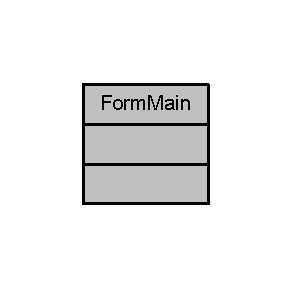
\includegraphics[width=140pt]{class_form_main__coll__graph}
\end{center}
\end{figure}


\subsection{Detailed Description}
Form\+Mainクラス 

The documentation for this class was generated from the following file\+:\begin{DoxyCompactItemize}
\item 
\hyperlink{_form_main_8cs}{Form\+Main.\+cs}\end{DoxyCompactItemize}

\hypertarget{class_reversi4color_form_1_1_hsl_color}{}\section{Reversi4color\+Form.\+Hsl\+Color Class Reference}
\label{class_reversi4color_form_1_1_hsl_color}\index{Reversi4color\+Form.\+Hsl\+Color@{Reversi4color\+Form.\+Hsl\+Color}}


H\+SL (H\+LS) カラーを表す  




Collaboration diagram for Reversi4color\+Form.\+Hsl\+Color\+:\nopagebreak
\begin{figure}[H]
\begin{center}
\leavevmode
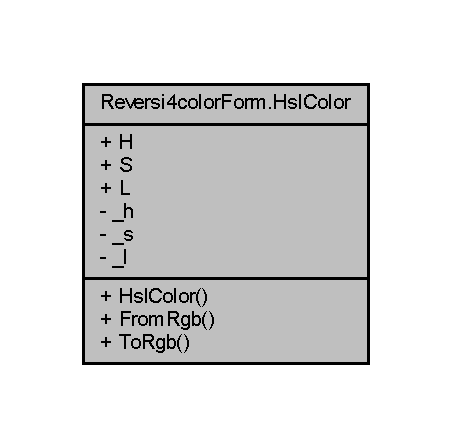
\includegraphics[width=217pt]{class_reversi4color_form_1_1_hsl_color__coll__graph}
\end{center}
\end{figure}
\subsection*{Public Member Functions}
\begin{DoxyCompactItemize}
\item 
\mbox{\Hypertarget{class_reversi4color_form_1_1_hsl_color_ad1bdb3fb711f7a0c5306ca92b3c189a3}\label{class_reversi4color_form_1_1_hsl_color_ad1bdb3fb711f7a0c5306ca92b3c189a3}} 
{\bfseries Hsl\+Color} (float hue, float saturation, float lightness)
\end{DoxyCompactItemize}
\subsection*{Static Public Member Functions}
\begin{DoxyCompactItemize}
\item 
static \hyperlink{class_reversi4color_form_1_1_hsl_color}{Hsl\+Color} \hyperlink{class_reversi4color_form_1_1_hsl_color_ae9adbbe822f39c29ef11839c80923718}{From\+Rgb} (Color rgb)
\begin{DoxyCompactList}\small\item\em 指定した\+Colorから\+Hsl\+Colorを作成する \end{DoxyCompactList}\item 
static Color \hyperlink{class_reversi4color_form_1_1_hsl_color_adc8d6bd6fd29eff44ccc1f2d1890fd72}{To\+Rgb} (\hyperlink{class_reversi4color_form_1_1_hsl_color}{Hsl\+Color} hsl)
\begin{DoxyCompactList}\small\item\em 指定した\+Hsl\+Colorから\+Colorを作成する \end{DoxyCompactList}\end{DoxyCompactItemize}
\subsection*{Properties}
\begin{DoxyCompactItemize}
\item 
float \hyperlink{class_reversi4color_form_1_1_hsl_color_a87a714cc5aa0034da10a51e6ebac4c16}{H}\hspace{0.3cm}{\ttfamily  \mbox{[}get\mbox{]}}
\begin{DoxyCompactList}\small\item\em 色相 (Hue) \end{DoxyCompactList}\item 
float \hyperlink{class_reversi4color_form_1_1_hsl_color_a6d0d1e94f3e7d2430ca58999a41ceabd}{S}\hspace{0.3cm}{\ttfamily  \mbox{[}get\mbox{]}}
\begin{DoxyCompactList}\small\item\em 彩度 (Saturation) \end{DoxyCompactList}\item 
float \hyperlink{class_reversi4color_form_1_1_hsl_color_a5d138402c61ef3bae7abe2c9c6d765dd}{L}\hspace{0.3cm}{\ttfamily  \mbox{[}get\mbox{]}}
\begin{DoxyCompactList}\small\item\em 輝度 (Lightness) \end{DoxyCompactList}\end{DoxyCompactItemize}
\subsection*{Private Attributes}
\begin{DoxyCompactItemize}
\item 
\mbox{\Hypertarget{class_reversi4color_form_1_1_hsl_color_af797949118aa18d14454f6c1d24e520b}\label{class_reversi4color_form_1_1_hsl_color_af797949118aa18d14454f6c1d24e520b}} 
float {\bfseries \+\_\+h}
\item 
\mbox{\Hypertarget{class_reversi4color_form_1_1_hsl_color_aac58e42c373ceb364180296ec5de9ef9}\label{class_reversi4color_form_1_1_hsl_color_aac58e42c373ceb364180296ec5de9ef9}} 
float {\bfseries \+\_\+s}
\item 
\mbox{\Hypertarget{class_reversi4color_form_1_1_hsl_color_aa4b98c49cacfb53aa337c72536a7d775}\label{class_reversi4color_form_1_1_hsl_color_aa4b98c49cacfb53aa337c72536a7d775}} 
float {\bfseries \+\_\+l}
\end{DoxyCompactItemize}


\subsection{Detailed Description}
H\+SL (H\+LS) カラーを表す 

Definition at line 28 of file Hsl\+Color.\+cs.



\subsection{Member Function Documentation}
\mbox{\Hypertarget{class_reversi4color_form_1_1_hsl_color_ae9adbbe822f39c29ef11839c80923718}\label{class_reversi4color_form_1_1_hsl_color_ae9adbbe822f39c29ef11839c80923718}} 
\index{Reversi4color\+Form\+::\+Hsl\+Color@{Reversi4color\+Form\+::\+Hsl\+Color}!From\+Rgb@{From\+Rgb}}
\index{From\+Rgb@{From\+Rgb}!Reversi4color\+Form\+::\+Hsl\+Color@{Reversi4color\+Form\+::\+Hsl\+Color}}
\subsubsection{\texorpdfstring{From\+Rgb()}{FromRgb()}}
{\footnotesize\ttfamily static \hyperlink{class_reversi4color_form_1_1_hsl_color}{Hsl\+Color} Reversi4color\+Form.\+Hsl\+Color.\+From\+Rgb (\begin{DoxyParamCaption}\item[{Color}]{rgb }\end{DoxyParamCaption})\hspace{0.3cm}{\ttfamily [static]}}



指定した\+Colorから\+Hsl\+Colorを作成する 


\begin{DoxyParams}{Parameters}
{\em rgb} & Color\\
\hline
\end{DoxyParams}
\begin{DoxyReturn}{Returns}
\hyperlink{class_reversi4color_form_1_1_hsl_color}{Hsl\+Color}
\end{DoxyReturn}


Definition at line 82 of file Hsl\+Color.\+cs.



Referenced by Reversi4color\+Form.\+Reversi.\+Draw\+Single\+Local().

Here is the caller graph for this function\+:\nopagebreak
\begin{figure}[H]
\begin{center}
\leavevmode
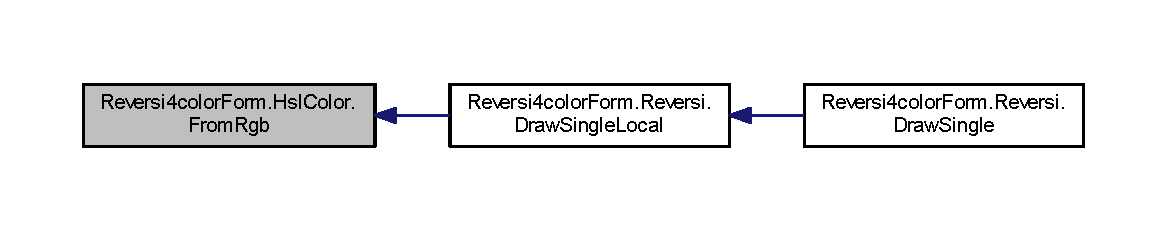
\includegraphics[width=350pt]{class_reversi4color_form_1_1_hsl_color_ae9adbbe822f39c29ef11839c80923718_icgraph}
\end{center}
\end{figure}
\mbox{\Hypertarget{class_reversi4color_form_1_1_hsl_color_adc8d6bd6fd29eff44ccc1f2d1890fd72}\label{class_reversi4color_form_1_1_hsl_color_adc8d6bd6fd29eff44ccc1f2d1890fd72}} 
\index{Reversi4color\+Form\+::\+Hsl\+Color@{Reversi4color\+Form\+::\+Hsl\+Color}!To\+Rgb@{To\+Rgb}}
\index{To\+Rgb@{To\+Rgb}!Reversi4color\+Form\+::\+Hsl\+Color@{Reversi4color\+Form\+::\+Hsl\+Color}}
\subsubsection{\texorpdfstring{To\+Rgb()}{ToRgb()}}
{\footnotesize\ttfamily static Color Reversi4color\+Form.\+Hsl\+Color.\+To\+Rgb (\begin{DoxyParamCaption}\item[{\hyperlink{class_reversi4color_form_1_1_hsl_color}{Hsl\+Color}}]{hsl }\end{DoxyParamCaption})\hspace{0.3cm}{\ttfamily [static]}}



指定した\+Hsl\+Colorから\+Colorを作成する 


\begin{DoxyParams}{Parameters}
{\em hsl} & \hyperlink{class_reversi4color_form_1_1_hsl_color}{Hsl\+Color}\\
\hline
\end{DoxyParams}
\begin{DoxyReturn}{Returns}
Color
\end{DoxyReturn}


Definition at line 141 of file Hsl\+Color.\+cs.



Referenced by Reversi4color\+Form.\+Reversi.\+Draw\+Single\+Local().

Here is the caller graph for this function\+:\nopagebreak
\begin{figure}[H]
\begin{center}
\leavevmode
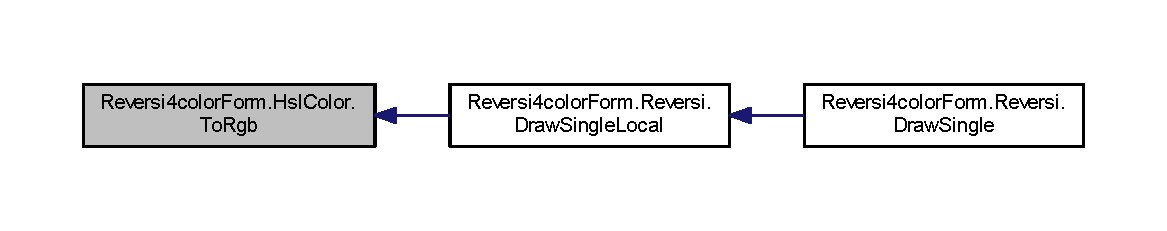
\includegraphics[width=350pt]{class_reversi4color_form_1_1_hsl_color_adc8d6bd6fd29eff44ccc1f2d1890fd72_icgraph}
\end{center}
\end{figure}


\subsection{Property Documentation}
\mbox{\Hypertarget{class_reversi4color_form_1_1_hsl_color_a87a714cc5aa0034da10a51e6ebac4c16}\label{class_reversi4color_form_1_1_hsl_color_a87a714cc5aa0034da10a51e6ebac4c16}} 
\index{Reversi4color\+Form\+::\+Hsl\+Color@{Reversi4color\+Form\+::\+Hsl\+Color}!H@{H}}
\index{H@{H}!Reversi4color\+Form\+::\+Hsl\+Color@{Reversi4color\+Form\+::\+Hsl\+Color}}
\subsubsection{\texorpdfstring{H}{H}}
{\footnotesize\ttfamily float Reversi4color\+Form.\+Hsl\+Color.\+H\hspace{0.3cm}{\ttfamily [get]}}



色相 (Hue) 



Definition at line 35 of file Hsl\+Color.\+cs.



Referenced by Reversi4color\+Form.\+Reversi.\+Draw\+Single\+Local(), and Reversi4color\+Form.\+Hsl\+Color.\+To\+Rgb().

\mbox{\Hypertarget{class_reversi4color_form_1_1_hsl_color_a5d138402c61ef3bae7abe2c9c6d765dd}\label{class_reversi4color_form_1_1_hsl_color_a5d138402c61ef3bae7abe2c9c6d765dd}} 
\index{Reversi4color\+Form\+::\+Hsl\+Color@{Reversi4color\+Form\+::\+Hsl\+Color}!L@{L}}
\index{L@{L}!Reversi4color\+Form\+::\+Hsl\+Color@{Reversi4color\+Form\+::\+Hsl\+Color}}
\subsubsection{\texorpdfstring{L}{L}}
{\footnotesize\ttfamily float Reversi4color\+Form.\+Hsl\+Color.\+L\hspace{0.3cm}{\ttfamily [get]}}



輝度 (Lightness) 



Definition at line 53 of file Hsl\+Color.\+cs.



Referenced by Reversi4color\+Form.\+Reversi.\+Draw\+Single\+Local(), and Reversi4color\+Form.\+Hsl\+Color.\+To\+Rgb().

\mbox{\Hypertarget{class_reversi4color_form_1_1_hsl_color_a6d0d1e94f3e7d2430ca58999a41ceabd}\label{class_reversi4color_form_1_1_hsl_color_a6d0d1e94f3e7d2430ca58999a41ceabd}} 
\index{Reversi4color\+Form\+::\+Hsl\+Color@{Reversi4color\+Form\+::\+Hsl\+Color}!S@{S}}
\index{S@{S}!Reversi4color\+Form\+::\+Hsl\+Color@{Reversi4color\+Form\+::\+Hsl\+Color}}
\subsubsection{\texorpdfstring{S}{S}}
{\footnotesize\ttfamily float Reversi4color\+Form.\+Hsl\+Color.\+S\hspace{0.3cm}{\ttfamily [get]}}



彩度 (Saturation) 



Definition at line 44 of file Hsl\+Color.\+cs.



Referenced by Reversi4color\+Form.\+Reversi.\+Draw\+Single\+Local(), and Reversi4color\+Form.\+Hsl\+Color.\+To\+Rgb().



The documentation for this class was generated from the following file\+:\begin{DoxyCompactItemize}
\item 
Model/\hyperlink{_hsl_color_8cs}{Hsl\+Color.\+cs}\end{DoxyCompactItemize}

\hypertarget{class_reversi4color_form_1_1_my_reversi}{}\section{Reversi4color\+Form.\+My\+Reversi Class Reference}
\label{class_reversi4color_form_1_1_my_reversi}\index{Reversi4color\+Form.\+My\+Reversi@{Reversi4color\+Form.\+My\+Reversi}}


リバーシクラス  




Collaboration diagram for Reversi4color\+Form.\+My\+Reversi\+:\nopagebreak
\begin{figure}[H]
\begin{center}
\leavevmode
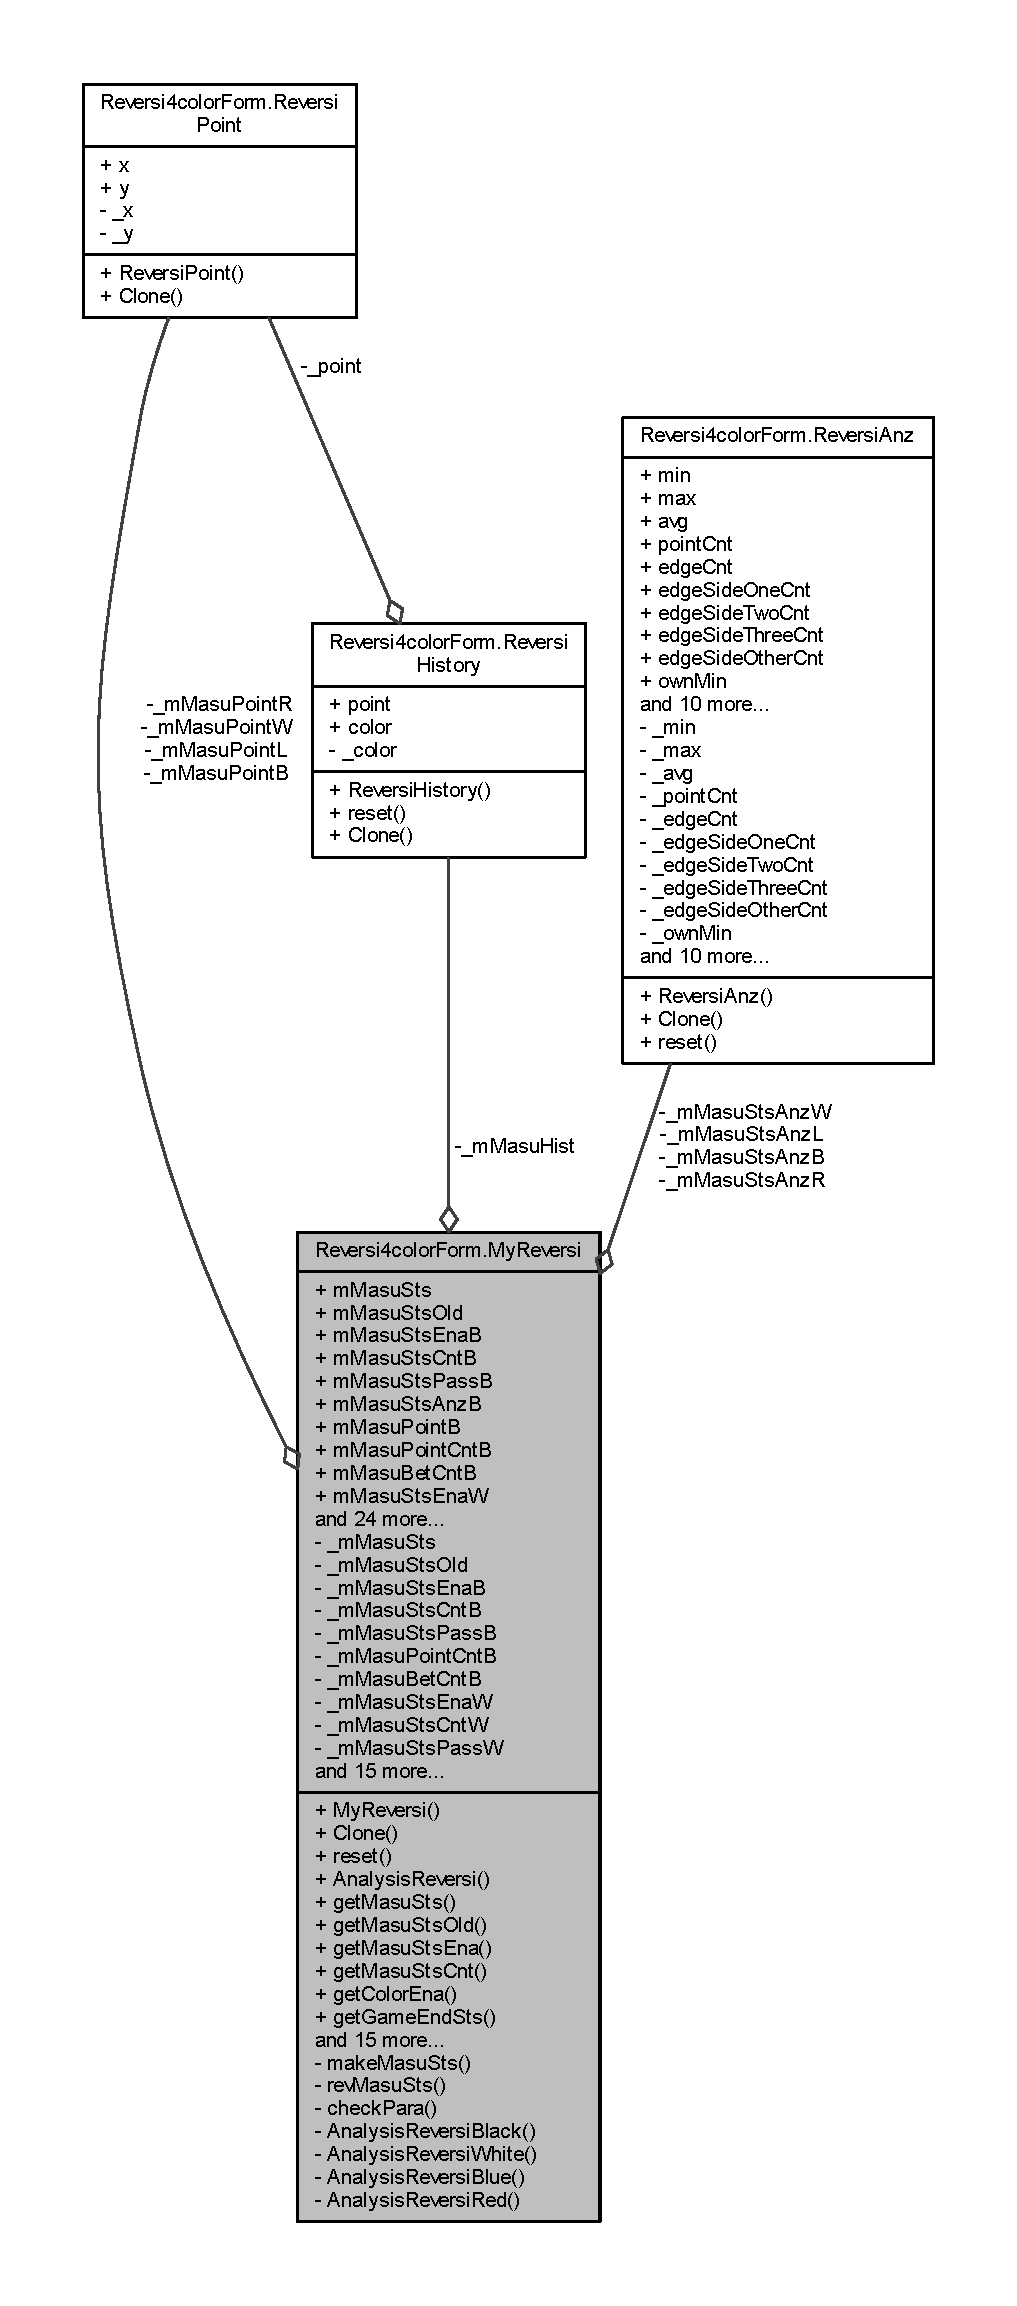
\includegraphics[height=550pt]{class_reversi4color_form_1_1_my_reversi__coll__graph}
\end{center}
\end{figure}
\subsection*{Public Member Functions}
\begin{DoxyCompactItemize}
\item 
\hyperlink{class_reversi4color_form_1_1_my_reversi_af58387f6a43abefc531e9098cdb5e08d}{My\+Reversi} (int masu\+Cnt, int masu\+Max)
\begin{DoxyCompactList}\small\item\em コンストラクタ \end{DoxyCompactList}\item 
\hyperlink{class_reversi4color_form_1_1_my_reversi}{My\+Reversi} \hyperlink{class_reversi4color_form_1_1_my_reversi_a45ce9de1a7d3209c2ad6c256ad1c4fe8}{Clone} ()
\begin{DoxyCompactList}\small\item\em コピー \end{DoxyCompactList}\item 
void \hyperlink{class_reversi4color_form_1_1_my_reversi_aeb24b855c540f99c901de08b11af1dd6}{reset} ()
\begin{DoxyCompactList}\small\item\em リセット \end{DoxyCompactList}\item 
void \hyperlink{class_reversi4color_form_1_1_my_reversi_ade9840e10e80b3e908a406efe9ee1372}{Analysis\+Reversi} (int b\+Pass\+Ena, int w\+Pass\+Ena, int l\+Pass\+Ena, int r\+Pass\+Ena)
\begin{DoxyCompactList}\small\item\em 解析を行う \end{DoxyCompactList}\item 
int \hyperlink{class_reversi4color_form_1_1_my_reversi_adc564d9d8aa75a871d33e09373485530}{get\+Masu\+Sts} (int y, int x)
\begin{DoxyCompactList}\small\item\em マスステータスを取得 \end{DoxyCompactList}\item 
int \hyperlink{class_reversi4color_form_1_1_my_reversi_aa56088eff96a48e68d4c7f688fe06b8d}{get\+Masu\+Sts\+Old} (int y, int x)
\begin{DoxyCompactList}\small\item\em 以前のマスステータスを取得 \end{DoxyCompactList}\item 
int \hyperlink{class_reversi4color_form_1_1_my_reversi_ac17f7f56dd24fa06ac8d394290feafef}{get\+Masu\+Sts\+Ena} (int color, int y, int x)
\begin{DoxyCompactList}\small\item\em 指定座標に指定色を置けるかチェック \end{DoxyCompactList}\item 
int \hyperlink{class_reversi4color_form_1_1_my_reversi_a5380e8f78bafedf7b0cdc86d943c8c22}{get\+Masu\+Sts\+Cnt} (int color, int y, int x)
\begin{DoxyCompactList}\small\item\em 指定座標の獲得コマ数取得 \end{DoxyCompactList}\item 
int \hyperlink{class_reversi4color_form_1_1_my_reversi_a5c18ae70cd8a10fee96f44e3a0e8621b}{get\+Color\+Ena} (int color)
\begin{DoxyCompactList}\small\item\em 指定色が現在置ける場所があるかチェック \end{DoxyCompactList}\item 
int \hyperlink{class_reversi4color_form_1_1_my_reversi_a5bdb21a8261d4af70bc2fabe7305ce22}{get\+Game\+End\+Sts} ()
\begin{DoxyCompactList}\small\item\em ゲーム終了かチェック \end{DoxyCompactList}\item 
int \hyperlink{class_reversi4color_form_1_1_my_reversi_a7b7f5f6c8ea7961a41cb3dcc4360c9d1}{set\+Masu\+Sts} (int color, int y, int x)
\begin{DoxyCompactList}\small\item\em 指定座標にコマを置く \end{DoxyCompactList}\item 
int \hyperlink{class_reversi4color_form_1_1_my_reversi_a099e2baa5bcf58eeeb0fe1cbe8be94d7}{set\+Masu\+Sts\+Forcibly} (int color, int y, int x)
\begin{DoxyCompactList}\small\item\em 指定座標にコマを強制的に置く \end{DoxyCompactList}\item 
int \hyperlink{class_reversi4color_form_1_1_my_reversi_ae612bc1a7a5ccbd972ce130de910e8e6}{set\+Masu\+Cnt} (int cnt)
\begin{DoxyCompactList}\small\item\em マスの数変更 \end{DoxyCompactList}\item 
\hyperlink{class_reversi4color_form_1_1_reversi_point}{Reversi\+Point} \hyperlink{class_reversi4color_form_1_1_my_reversi_a5af52fd8272221e7fecfc8375a9f7be2}{get\+Point} (int color, int num)
\begin{DoxyCompactList}\small\item\em ポイント座標取得 \end{DoxyCompactList}\item 
int \hyperlink{class_reversi4color_form_1_1_my_reversi_a64db9e5d07901c13e985e1730816bb25}{get\+Point\+Cnt} (int color)
\begin{DoxyCompactList}\small\item\em ポイント座標数取得 \end{DoxyCompactList}\item 
int \hyperlink{class_reversi4color_form_1_1_my_reversi_ae184f1817b7dfac87613179e3e7e9124}{get\+Bet\+Cnt} (int color)
\begin{DoxyCompactList}\small\item\em コマ数取得 \end{DoxyCompactList}\item 
int \hyperlink{class_reversi4color_form_1_1_my_reversi_accf9e5107a9e029db4f4ba2968800d44}{get\+Pass\+Ena} (int color, int y, int x)
\begin{DoxyCompactList}\small\item\em パス判定 \end{DoxyCompactList}\item 
\hyperlink{class_reversi4color_form_1_1_reversi_history}{Reversi\+History} \hyperlink{class_reversi4color_form_1_1_my_reversi_a6765e90e98f20c7a19a941400446d006}{get\+History} (int num)
\begin{DoxyCompactList}\small\item\em 履歴取得 \end{DoxyCompactList}\item 
int \hyperlink{class_reversi4color_form_1_1_my_reversi_a9d4345e1a06f0d94f073f82037aa6113}{get\+History\+Cnt} ()
\begin{DoxyCompactList}\small\item\em 履歴数取得 \end{DoxyCompactList}\item 
\hyperlink{class_reversi4color_form_1_1_reversi_anz}{Reversi\+Anz} \hyperlink{class_reversi4color_form_1_1_my_reversi_ad0027ead546dfa8a7844e54fb0dddfab}{get\+Point\+Anz} (int color, int y, int x)
\begin{DoxyCompactList}\small\item\em ポイント座標解析取得 \end{DoxyCompactList}\item 
int \hyperlink{class_reversi4color_form_1_1_my_reversi_a8538a52d715eb754c49fc5719390d035}{check\+Edge} (int color, int y, int x)
\begin{DoxyCompactList}\small\item\em 角の隣に置いても角を取られないマス検索 \end{DoxyCompactList}\item 
int \hyperlink{class_reversi4color_form_1_1_my_reversi_a634f9e5deab1d15b929a33012acd03c2}{get\+Edge\+Side\+Zero} (int y, int x)
\begin{DoxyCompactList}\small\item\em 指定座標が角か取得 \end{DoxyCompactList}\item 
int \hyperlink{class_reversi4color_form_1_1_my_reversi_abf9583e4d29970acf85e662eb8a273dc}{get\+Edge\+Side\+One} (int y, int x)
\begin{DoxyCompactList}\small\item\em 指定座標が角の一つ手前か取得 \end{DoxyCompactList}\item 
int \hyperlink{class_reversi4color_form_1_1_my_reversi_af5ccb42b478bf692989daef9c2495c53}{get\+Edge\+Side\+Two} (int y, int x)
\begin{DoxyCompactList}\small\item\em 指定座標が角の二つ手前か取得 \end{DoxyCompactList}\item 
int \hyperlink{class_reversi4color_form_1_1_my_reversi_aca70a03939805aceed92fabb4a00636b}{get\+Edge\+Side\+Three} (int y, int x)
\begin{DoxyCompactList}\small\item\em 指定座標が角の三つ以上手前か取得 \end{DoxyCompactList}\end{DoxyCompactItemize}
\subsection*{Properties}
\begin{DoxyCompactItemize}
\item 
\mbox{\Hypertarget{class_reversi4color_form_1_1_my_reversi_afcb4f036650401789ef6e21831482951}\label{class_reversi4color_form_1_1_my_reversi_afcb4f036650401789ef6e21831482951}} 
int \mbox{[},\mbox{]} {\bfseries m\+Masu\+Sts}\hspace{0.3cm}{\ttfamily  \mbox{[}get, set\mbox{]}}
\item 
\mbox{\Hypertarget{class_reversi4color_form_1_1_my_reversi_a73b9d86fd8d459a873e1289be185d917}\label{class_reversi4color_form_1_1_my_reversi_a73b9d86fd8d459a873e1289be185d917}} 
int \mbox{[},\mbox{]} {\bfseries m\+Masu\+Sts\+Old}\hspace{0.3cm}{\ttfamily  \mbox{[}get, set\mbox{]}}
\item 
\mbox{\Hypertarget{class_reversi4color_form_1_1_my_reversi_abbae0a78ff6311684d4bc46eacf73e69}\label{class_reversi4color_form_1_1_my_reversi_abbae0a78ff6311684d4bc46eacf73e69}} 
int \mbox{[},\mbox{]} {\bfseries m\+Masu\+Sts\+EnaB}\hspace{0.3cm}{\ttfamily  \mbox{[}get, set\mbox{]}}
\item 
\mbox{\Hypertarget{class_reversi4color_form_1_1_my_reversi_aac15428fd38da9d9070f2d0a6591a1f8}\label{class_reversi4color_form_1_1_my_reversi_aac15428fd38da9d9070f2d0a6591a1f8}} 
int \mbox{[},\mbox{]} {\bfseries m\+Masu\+Sts\+CntB}\hspace{0.3cm}{\ttfamily  \mbox{[}get, set\mbox{]}}
\item 
\mbox{\Hypertarget{class_reversi4color_form_1_1_my_reversi_a6e52c525b66dbe22a472b4395d5cad23}\label{class_reversi4color_form_1_1_my_reversi_a6e52c525b66dbe22a472b4395d5cad23}} 
int \mbox{[},\mbox{]} {\bfseries m\+Masu\+Sts\+PassB}\hspace{0.3cm}{\ttfamily  \mbox{[}get, set\mbox{]}}
\item 
\mbox{\Hypertarget{class_reversi4color_form_1_1_my_reversi_ae362f54640eb98f354eca40bbb71dca9}\label{class_reversi4color_form_1_1_my_reversi_ae362f54640eb98f354eca40bbb71dca9}} 
\hyperlink{class_reversi4color_form_1_1_reversi_anz}{Reversi\+Anz} \mbox{[},\mbox{]} {\bfseries m\+Masu\+Sts\+AnzB}\hspace{0.3cm}{\ttfamily  \mbox{[}get, set\mbox{]}}
\item 
\mbox{\Hypertarget{class_reversi4color_form_1_1_my_reversi_a384a1d778b0cc80485b032a6bf866266}\label{class_reversi4color_form_1_1_my_reversi_a384a1d778b0cc80485b032a6bf866266}} 
\hyperlink{class_reversi4color_form_1_1_reversi_point}{Reversi\+Point} \mbox{[}$\,$\mbox{]} {\bfseries m\+Masu\+PointB}\hspace{0.3cm}{\ttfamily  \mbox{[}get, set\mbox{]}}
\item 
\mbox{\Hypertarget{class_reversi4color_form_1_1_my_reversi_a56254c917e1ba9bf6473abbc997dec42}\label{class_reversi4color_form_1_1_my_reversi_a56254c917e1ba9bf6473abbc997dec42}} 
int {\bfseries m\+Masu\+Point\+CntB}\hspace{0.3cm}{\ttfamily  \mbox{[}get, set\mbox{]}}
\item 
\mbox{\Hypertarget{class_reversi4color_form_1_1_my_reversi_aaa405094e77406e2ef5f0f00bcabee6c}\label{class_reversi4color_form_1_1_my_reversi_aaa405094e77406e2ef5f0f00bcabee6c}} 
int {\bfseries m\+Masu\+Bet\+CntB}\hspace{0.3cm}{\ttfamily  \mbox{[}get, set\mbox{]}}
\item 
\mbox{\Hypertarget{class_reversi4color_form_1_1_my_reversi_aa5e95baf2380943c873c52a1ed2b648b}\label{class_reversi4color_form_1_1_my_reversi_aa5e95baf2380943c873c52a1ed2b648b}} 
int \mbox{[},\mbox{]} {\bfseries m\+Masu\+Sts\+EnaW}\hspace{0.3cm}{\ttfamily  \mbox{[}get, set\mbox{]}}
\item 
\mbox{\Hypertarget{class_reversi4color_form_1_1_my_reversi_abd1cfe7d8ba51430264703363a3a5225}\label{class_reversi4color_form_1_1_my_reversi_abd1cfe7d8ba51430264703363a3a5225}} 
int \mbox{[},\mbox{]} {\bfseries m\+Masu\+Sts\+CntW}\hspace{0.3cm}{\ttfamily  \mbox{[}get, set\mbox{]}}
\item 
\mbox{\Hypertarget{class_reversi4color_form_1_1_my_reversi_aa3f84bdfae5b84f1f0ec5eb93b96d764}\label{class_reversi4color_form_1_1_my_reversi_aa3f84bdfae5b84f1f0ec5eb93b96d764}} 
int \mbox{[},\mbox{]} {\bfseries m\+Masu\+Sts\+PassW}\hspace{0.3cm}{\ttfamily  \mbox{[}get, set\mbox{]}}
\item 
\mbox{\Hypertarget{class_reversi4color_form_1_1_my_reversi_a1d2a5f81ee975d634fefb7e168db53fb}\label{class_reversi4color_form_1_1_my_reversi_a1d2a5f81ee975d634fefb7e168db53fb}} 
\hyperlink{class_reversi4color_form_1_1_reversi_anz}{Reversi\+Anz} \mbox{[},\mbox{]} {\bfseries m\+Masu\+Sts\+AnzW}\hspace{0.3cm}{\ttfamily  \mbox{[}get, set\mbox{]}}
\item 
\mbox{\Hypertarget{class_reversi4color_form_1_1_my_reversi_ac358b2d12a305066404674b1364c685d}\label{class_reversi4color_form_1_1_my_reversi_ac358b2d12a305066404674b1364c685d}} 
\hyperlink{class_reversi4color_form_1_1_reversi_point}{Reversi\+Point} \mbox{[}$\,$\mbox{]} {\bfseries m\+Masu\+PointW}\hspace{0.3cm}{\ttfamily  \mbox{[}get, set\mbox{]}}
\item 
\mbox{\Hypertarget{class_reversi4color_form_1_1_my_reversi_abde3d63d384d2c0c1b0b07304543bead}\label{class_reversi4color_form_1_1_my_reversi_abde3d63d384d2c0c1b0b07304543bead}} 
int {\bfseries m\+Masu\+Point\+CntW}\hspace{0.3cm}{\ttfamily  \mbox{[}get, set\mbox{]}}
\item 
\mbox{\Hypertarget{class_reversi4color_form_1_1_my_reversi_a604576daafd52082e84b4ee6ee788366}\label{class_reversi4color_form_1_1_my_reversi_a604576daafd52082e84b4ee6ee788366}} 
int {\bfseries m\+Masu\+Bet\+CntW}\hspace{0.3cm}{\ttfamily  \mbox{[}get, set\mbox{]}}
\item 
\mbox{\Hypertarget{class_reversi4color_form_1_1_my_reversi_a30940f5d666c12cf4cac621be1ca5fd9}\label{class_reversi4color_form_1_1_my_reversi_a30940f5d666c12cf4cac621be1ca5fd9}} 
int \mbox{[},\mbox{]} {\bfseries m\+Masu\+Sts\+EnaL}\hspace{0.3cm}{\ttfamily  \mbox{[}get, set\mbox{]}}
\item 
\mbox{\Hypertarget{class_reversi4color_form_1_1_my_reversi_acfb803e8b614517fafba883f94178c74}\label{class_reversi4color_form_1_1_my_reversi_acfb803e8b614517fafba883f94178c74}} 
int \mbox{[},\mbox{]} {\bfseries m\+Masu\+Sts\+CntL}\hspace{0.3cm}{\ttfamily  \mbox{[}get, set\mbox{]}}
\item 
\mbox{\Hypertarget{class_reversi4color_form_1_1_my_reversi_ac6eb01e80ae36b065f6fc965ec329d32}\label{class_reversi4color_form_1_1_my_reversi_ac6eb01e80ae36b065f6fc965ec329d32}} 
int \mbox{[},\mbox{]} {\bfseries m\+Masu\+Sts\+PassL}\hspace{0.3cm}{\ttfamily  \mbox{[}get, set\mbox{]}}
\item 
\mbox{\Hypertarget{class_reversi4color_form_1_1_my_reversi_a716eba091ed38e3b07087402d9d34f9f}\label{class_reversi4color_form_1_1_my_reversi_a716eba091ed38e3b07087402d9d34f9f}} 
\hyperlink{class_reversi4color_form_1_1_reversi_anz}{Reversi\+Anz} \mbox{[},\mbox{]} {\bfseries m\+Masu\+Sts\+AnzL}\hspace{0.3cm}{\ttfamily  \mbox{[}get, set\mbox{]}}
\item 
\mbox{\Hypertarget{class_reversi4color_form_1_1_my_reversi_ad1415da3f09e70765e46a15b3e67e5f1}\label{class_reversi4color_form_1_1_my_reversi_ad1415da3f09e70765e46a15b3e67e5f1}} 
\hyperlink{class_reversi4color_form_1_1_reversi_point}{Reversi\+Point} \mbox{[}$\,$\mbox{]} {\bfseries m\+Masu\+PointL}\hspace{0.3cm}{\ttfamily  \mbox{[}get, set\mbox{]}}
\item 
\mbox{\Hypertarget{class_reversi4color_form_1_1_my_reversi_a75262a424ab0be6d1391db712172f0f7}\label{class_reversi4color_form_1_1_my_reversi_a75262a424ab0be6d1391db712172f0f7}} 
int {\bfseries m\+Masu\+Point\+CntL}\hspace{0.3cm}{\ttfamily  \mbox{[}get, set\mbox{]}}
\item 
\mbox{\Hypertarget{class_reversi4color_form_1_1_my_reversi_ab8c38b5da80f2f2f572ccc56aa02d949}\label{class_reversi4color_form_1_1_my_reversi_ab8c38b5da80f2f2f572ccc56aa02d949}} 
int {\bfseries m\+Masu\+Bet\+CntL}\hspace{0.3cm}{\ttfamily  \mbox{[}get, set\mbox{]}}
\item 
\mbox{\Hypertarget{class_reversi4color_form_1_1_my_reversi_ad948c4a1979d3498c1013bed22529fe2}\label{class_reversi4color_form_1_1_my_reversi_ad948c4a1979d3498c1013bed22529fe2}} 
int \mbox{[},\mbox{]} {\bfseries m\+Masu\+Sts\+EnaR}\hspace{0.3cm}{\ttfamily  \mbox{[}get, set\mbox{]}}
\item 
\mbox{\Hypertarget{class_reversi4color_form_1_1_my_reversi_a96a3121344b6c3589522812f08207faf}\label{class_reversi4color_form_1_1_my_reversi_a96a3121344b6c3589522812f08207faf}} 
int \mbox{[},\mbox{]} {\bfseries m\+Masu\+Sts\+CntR}\hspace{0.3cm}{\ttfamily  \mbox{[}get, set\mbox{]}}
\item 
\mbox{\Hypertarget{class_reversi4color_form_1_1_my_reversi_a400f23de0d5f509b7397c15c60d27bb4}\label{class_reversi4color_form_1_1_my_reversi_a400f23de0d5f509b7397c15c60d27bb4}} 
int \mbox{[},\mbox{]} {\bfseries m\+Masu\+Sts\+PassR}\hspace{0.3cm}{\ttfamily  \mbox{[}get, set\mbox{]}}
\item 
\mbox{\Hypertarget{class_reversi4color_form_1_1_my_reversi_a0b5048e91d8d6944d2ed644cf79eb7dd}\label{class_reversi4color_form_1_1_my_reversi_a0b5048e91d8d6944d2ed644cf79eb7dd}} 
\hyperlink{class_reversi4color_form_1_1_reversi_anz}{Reversi\+Anz} \mbox{[},\mbox{]} {\bfseries m\+Masu\+Sts\+AnzR}\hspace{0.3cm}{\ttfamily  \mbox{[}get, set\mbox{]}}
\item 
\mbox{\Hypertarget{class_reversi4color_form_1_1_my_reversi_a9c8e793beeb3af9572c5cb62d50d2263}\label{class_reversi4color_form_1_1_my_reversi_a9c8e793beeb3af9572c5cb62d50d2263}} 
\hyperlink{class_reversi4color_form_1_1_reversi_point}{Reversi\+Point} \mbox{[}$\,$\mbox{]} {\bfseries m\+Masu\+PointR}\hspace{0.3cm}{\ttfamily  \mbox{[}get, set\mbox{]}}
\item 
\mbox{\Hypertarget{class_reversi4color_form_1_1_my_reversi_a9b3cd7a414525ce7ea035b260b078d9e}\label{class_reversi4color_form_1_1_my_reversi_a9b3cd7a414525ce7ea035b260b078d9e}} 
int {\bfseries m\+Masu\+Point\+CntR}\hspace{0.3cm}{\ttfamily  \mbox{[}get, set\mbox{]}}
\item 
\mbox{\Hypertarget{class_reversi4color_form_1_1_my_reversi_a9adc9b4911feccee1165c6aa5470d37f}\label{class_reversi4color_form_1_1_my_reversi_a9adc9b4911feccee1165c6aa5470d37f}} 
int {\bfseries m\+Masu\+Bet\+CntR}\hspace{0.3cm}{\ttfamily  \mbox{[}get, set\mbox{]}}
\item 
\mbox{\Hypertarget{class_reversi4color_form_1_1_my_reversi_aadc69426303cf45406f9c9e6e8c4a3fc}\label{class_reversi4color_form_1_1_my_reversi_aadc69426303cf45406f9c9e6e8c4a3fc}} 
int {\bfseries m\+Masu\+Cnt}\hspace{0.3cm}{\ttfamily  \mbox{[}get, set\mbox{]}}
\item 
\mbox{\Hypertarget{class_reversi4color_form_1_1_my_reversi_a0af2e95eadcf42d4e1225946b6fd2da8}\label{class_reversi4color_form_1_1_my_reversi_a0af2e95eadcf42d4e1225946b6fd2da8}} 
int {\bfseries m\+Masu\+Cnt\+Max}\hspace{0.3cm}{\ttfamily  \mbox{[}get, set\mbox{]}}
\item 
\mbox{\Hypertarget{class_reversi4color_form_1_1_my_reversi_acf5dc58f9a8250462b04e945b20dc6d6}\label{class_reversi4color_form_1_1_my_reversi_acf5dc58f9a8250462b04e945b20dc6d6}} 
int {\bfseries m\+Masu\+Hist\+Cur}\hspace{0.3cm}{\ttfamily  \mbox{[}get, set\mbox{]}}
\item 
\mbox{\Hypertarget{class_reversi4color_form_1_1_my_reversi_abc425abe7a7564eacab7589bff8d57fa}\label{class_reversi4color_form_1_1_my_reversi_abc425abe7a7564eacab7589bff8d57fa}} 
\hyperlink{class_reversi4color_form_1_1_reversi_history}{Reversi\+History} \mbox{[}$\,$\mbox{]} {\bfseries m\+Masu\+Hist}\hspace{0.3cm}{\ttfamily  \mbox{[}get, set\mbox{]}}
\end{DoxyCompactItemize}
\subsection*{Private Member Functions}
\begin{DoxyCompactItemize}
\item 
int \hyperlink{class_reversi4color_form_1_1_my_reversi_afdfd5f0fc3a4ed4e24bcf67ead0bb980}{make\+Masu\+Sts} (int color)
\begin{DoxyCompactList}\small\item\em 各コマの置ける場所等のステータス作成 \end{DoxyCompactList}\item 
void \hyperlink{class_reversi4color_form_1_1_my_reversi_a94536b8feaa37ca51b3d0612befae12f}{rev\+Masu\+Sts} (int color, int y, int x)
\begin{DoxyCompactList}\small\item\em コマをひっくり返す \end{DoxyCompactList}\item 
int \hyperlink{class_reversi4color_form_1_1_my_reversi_a02c145ac89302f2360cdb0c0391a38ce}{check\+Para} (int para, int min, int max)
\begin{DoxyCompactList}\small\item\em パラメーター範囲チェック \end{DoxyCompactList}\item 
void \hyperlink{class_reversi4color_form_1_1_my_reversi_ae4c0b7e9a3cedba827facf1d96b654f0}{Analysis\+Reversi\+Black} ()
\begin{DoxyCompactList}\small\item\em 解析を行う(黒) \end{DoxyCompactList}\item 
void \hyperlink{class_reversi4color_form_1_1_my_reversi_a61ca891ff78c7357ab077ce7bd3cbf97}{Analysis\+Reversi\+White} ()
\begin{DoxyCompactList}\small\item\em 解析を行う(白) \end{DoxyCompactList}\item 
void \hyperlink{class_reversi4color_form_1_1_my_reversi_a07c18a7adbcc3bd0993673f0a8f63c85}{Analysis\+Reversi\+Blue} ()
\begin{DoxyCompactList}\small\item\em 解析を行う(青) \end{DoxyCompactList}\item 
void \hyperlink{class_reversi4color_form_1_1_my_reversi_a2d0c12ed7036def583e06ca4df37f367}{Analysis\+Reversi\+Red} ()
\begin{DoxyCompactList}\small\item\em 解析を行う(赤) \end{DoxyCompactList}\end{DoxyCompactItemize}
\subsection*{Private Attributes}
\begin{DoxyCompactItemize}
\item 
\mbox{\Hypertarget{class_reversi4color_form_1_1_my_reversi_a3d9d8bfb90c04503cb633e79c52e15f6}\label{class_reversi4color_form_1_1_my_reversi_a3d9d8bfb90c04503cb633e79c52e15f6}} 
int \mbox{[},\mbox{]} \hyperlink{class_reversi4color_form_1_1_my_reversi_a3d9d8bfb90c04503cb633e79c52e15f6}{\+\_\+m\+Masu\+Sts}
\begin{DoxyCompactList}\small\item\em マスの状態 \end{DoxyCompactList}\item 
\mbox{\Hypertarget{class_reversi4color_form_1_1_my_reversi_ae2fe1edfa4dbd6757f80c405da47bc0e}\label{class_reversi4color_form_1_1_my_reversi_ae2fe1edfa4dbd6757f80c405da47bc0e}} 
int \mbox{[},\mbox{]} \hyperlink{class_reversi4color_form_1_1_my_reversi_ae2fe1edfa4dbd6757f80c405da47bc0e}{\+\_\+m\+Masu\+Sts\+Old}
\begin{DoxyCompactList}\small\item\em 以前のマスの状態 \end{DoxyCompactList}\item 
\mbox{\Hypertarget{class_reversi4color_form_1_1_my_reversi_ad86b7fdf96815f0679eacf49f0c060f4}\label{class_reversi4color_form_1_1_my_reversi_ad86b7fdf96815f0679eacf49f0c060f4}} 
int \mbox{[},\mbox{]} \hyperlink{class_reversi4color_form_1_1_my_reversi_ad86b7fdf96815f0679eacf49f0c060f4}{\+\_\+m\+Masu\+Sts\+EnaB}
\begin{DoxyCompactList}\small\item\em 黒の置ける場所 \end{DoxyCompactList}\item 
\mbox{\Hypertarget{class_reversi4color_form_1_1_my_reversi_a3918babf996c0c954033f503eda7a263}\label{class_reversi4color_form_1_1_my_reversi_a3918babf996c0c954033f503eda7a263}} 
int \mbox{[},\mbox{]} \hyperlink{class_reversi4color_form_1_1_my_reversi_a3918babf996c0c954033f503eda7a263}{\+\_\+m\+Masu\+Sts\+CntB}
\begin{DoxyCompactList}\small\item\em 黒の獲得コマ数 \end{DoxyCompactList}\item 
\mbox{\Hypertarget{class_reversi4color_form_1_1_my_reversi_af966c44de228f71184114079aecb7af1}\label{class_reversi4color_form_1_1_my_reversi_af966c44de228f71184114079aecb7af1}} 
int \mbox{[},\mbox{]} \hyperlink{class_reversi4color_form_1_1_my_reversi_af966c44de228f71184114079aecb7af1}{\+\_\+m\+Masu\+Sts\+PassB}
\begin{DoxyCompactList}\small\item\em 黒が相手をパスさせる場所 \end{DoxyCompactList}\item 
\mbox{\Hypertarget{class_reversi4color_form_1_1_my_reversi_a550efa04abf05ea9d96a853b681c9be1}\label{class_reversi4color_form_1_1_my_reversi_a550efa04abf05ea9d96a853b681c9be1}} 
\hyperlink{class_reversi4color_form_1_1_reversi_anz}{Reversi\+Anz} \mbox{[},\mbox{]} \hyperlink{class_reversi4color_form_1_1_my_reversi_a550efa04abf05ea9d96a853b681c9be1}{\+\_\+m\+Masu\+Sts\+AnzB}
\begin{DoxyCompactList}\small\item\em 黒がその場所に置いた場合の解析結果 \end{DoxyCompactList}\item 
\mbox{\Hypertarget{class_reversi4color_form_1_1_my_reversi_ac9bc4d4325e20448773ee4b9cfdd6430}\label{class_reversi4color_form_1_1_my_reversi_ac9bc4d4325e20448773ee4b9cfdd6430}} 
\hyperlink{class_reversi4color_form_1_1_reversi_point}{Reversi\+Point} \mbox{[}$\,$\mbox{]} \hyperlink{class_reversi4color_form_1_1_my_reversi_ac9bc4d4325e20448773ee4b9cfdd6430}{\+\_\+m\+Masu\+PointB}
\begin{DoxyCompactList}\small\item\em 黒の置ける場所座標一覧 \end{DoxyCompactList}\item 
\mbox{\Hypertarget{class_reversi4color_form_1_1_my_reversi_ae88cc7951561a3e5b3fbcacf61513906}\label{class_reversi4color_form_1_1_my_reversi_ae88cc7951561a3e5b3fbcacf61513906}} 
int \hyperlink{class_reversi4color_form_1_1_my_reversi_ae88cc7951561a3e5b3fbcacf61513906}{\+\_\+m\+Masu\+Point\+CntB}
\begin{DoxyCompactList}\small\item\em 黒の置ける場所座標一覧数 \end{DoxyCompactList}\item 
\mbox{\Hypertarget{class_reversi4color_form_1_1_my_reversi_a83d51a35e6d21a112fbcef3a5a624da1}\label{class_reversi4color_form_1_1_my_reversi_a83d51a35e6d21a112fbcef3a5a624da1}} 
int \hyperlink{class_reversi4color_form_1_1_my_reversi_a83d51a35e6d21a112fbcef3a5a624da1}{\+\_\+m\+Masu\+Bet\+CntB}
\begin{DoxyCompactList}\small\item\em 黒コマ数 \end{DoxyCompactList}\item 
\mbox{\Hypertarget{class_reversi4color_form_1_1_my_reversi_ad80081db3aa0ab2b758113964869cea3}\label{class_reversi4color_form_1_1_my_reversi_ad80081db3aa0ab2b758113964869cea3}} 
int \mbox{[},\mbox{]} \hyperlink{class_reversi4color_form_1_1_my_reversi_ad80081db3aa0ab2b758113964869cea3}{\+\_\+m\+Masu\+Sts\+EnaW}
\begin{DoxyCompactList}\small\item\em 白の置ける場所 \end{DoxyCompactList}\item 
\mbox{\Hypertarget{class_reversi4color_form_1_1_my_reversi_aff624d92131f9a613e77345e40b3bb4e}\label{class_reversi4color_form_1_1_my_reversi_aff624d92131f9a613e77345e40b3bb4e}} 
int \mbox{[},\mbox{]} \hyperlink{class_reversi4color_form_1_1_my_reversi_aff624d92131f9a613e77345e40b3bb4e}{\+\_\+m\+Masu\+Sts\+CntW}
\begin{DoxyCompactList}\small\item\em 白の獲得コマ数 \end{DoxyCompactList}\item 
\mbox{\Hypertarget{class_reversi4color_form_1_1_my_reversi_a89f7e415682c41840573f10a6e7edc3d}\label{class_reversi4color_form_1_1_my_reversi_a89f7e415682c41840573f10a6e7edc3d}} 
int \mbox{[},\mbox{]} \hyperlink{class_reversi4color_form_1_1_my_reversi_a89f7e415682c41840573f10a6e7edc3d}{\+\_\+m\+Masu\+Sts\+PassW}
\begin{DoxyCompactList}\small\item\em 白が相手をパスさせる場所 \end{DoxyCompactList}\item 
\mbox{\Hypertarget{class_reversi4color_form_1_1_my_reversi_a66a856b8080442b4f252390cacc2ef52}\label{class_reversi4color_form_1_1_my_reversi_a66a856b8080442b4f252390cacc2ef52}} 
\hyperlink{class_reversi4color_form_1_1_reversi_anz}{Reversi\+Anz} \mbox{[},\mbox{]} \hyperlink{class_reversi4color_form_1_1_my_reversi_a66a856b8080442b4f252390cacc2ef52}{\+\_\+m\+Masu\+Sts\+AnzW}
\begin{DoxyCompactList}\small\item\em 白がその場所に置いた場合の解析結果 \end{DoxyCompactList}\item 
\mbox{\Hypertarget{class_reversi4color_form_1_1_my_reversi_aa7c26205f65aebc48e6679222159b673}\label{class_reversi4color_form_1_1_my_reversi_aa7c26205f65aebc48e6679222159b673}} 
\hyperlink{class_reversi4color_form_1_1_reversi_point}{Reversi\+Point} \mbox{[}$\,$\mbox{]} \hyperlink{class_reversi4color_form_1_1_my_reversi_aa7c26205f65aebc48e6679222159b673}{\+\_\+m\+Masu\+PointW}
\begin{DoxyCompactList}\small\item\em 白の置ける場所座標一覧 \end{DoxyCompactList}\item 
\mbox{\Hypertarget{class_reversi4color_form_1_1_my_reversi_aa7d054ccd9f9901a033a18332086a10a}\label{class_reversi4color_form_1_1_my_reversi_aa7d054ccd9f9901a033a18332086a10a}} 
int \hyperlink{class_reversi4color_form_1_1_my_reversi_aa7d054ccd9f9901a033a18332086a10a}{\+\_\+m\+Masu\+Point\+CntW}
\begin{DoxyCompactList}\small\item\em 白の置ける場所座標一覧数 \end{DoxyCompactList}\item 
\mbox{\Hypertarget{class_reversi4color_form_1_1_my_reversi_a680a874c7a11af0831ce4af93e5557f4}\label{class_reversi4color_form_1_1_my_reversi_a680a874c7a11af0831ce4af93e5557f4}} 
int \hyperlink{class_reversi4color_form_1_1_my_reversi_a680a874c7a11af0831ce4af93e5557f4}{\+\_\+m\+Masu\+Bet\+CntW}
\begin{DoxyCompactList}\small\item\em 白コマ数 \end{DoxyCompactList}\item 
\mbox{\Hypertarget{class_reversi4color_form_1_1_my_reversi_a110dc44cfb374cb14cdaca56134e3c03}\label{class_reversi4color_form_1_1_my_reversi_a110dc44cfb374cb14cdaca56134e3c03}} 
int \mbox{[},\mbox{]} \hyperlink{class_reversi4color_form_1_1_my_reversi_a110dc44cfb374cb14cdaca56134e3c03}{\+\_\+m\+Masu\+Sts\+EnaL}
\begin{DoxyCompactList}\small\item\em 青の置ける場所 \end{DoxyCompactList}\item 
\mbox{\Hypertarget{class_reversi4color_form_1_1_my_reversi_ad2e537dcf896b3a59585ea3b860118eb}\label{class_reversi4color_form_1_1_my_reversi_ad2e537dcf896b3a59585ea3b860118eb}} 
int \mbox{[},\mbox{]} \hyperlink{class_reversi4color_form_1_1_my_reversi_ad2e537dcf896b3a59585ea3b860118eb}{\+\_\+m\+Masu\+Sts\+CntL}
\begin{DoxyCompactList}\small\item\em 青の獲得コマ数 \end{DoxyCompactList}\item 
\mbox{\Hypertarget{class_reversi4color_form_1_1_my_reversi_adec39a5d5520b6936be5924514ea2e7c}\label{class_reversi4color_form_1_1_my_reversi_adec39a5d5520b6936be5924514ea2e7c}} 
int \mbox{[},\mbox{]} \hyperlink{class_reversi4color_form_1_1_my_reversi_adec39a5d5520b6936be5924514ea2e7c}{\+\_\+m\+Masu\+Sts\+PassL}
\begin{DoxyCompactList}\small\item\em 青が相手をパスさせる場所 \end{DoxyCompactList}\item 
\mbox{\Hypertarget{class_reversi4color_form_1_1_my_reversi_a47fa6ace5cf0a134b24062ffcd44046e}\label{class_reversi4color_form_1_1_my_reversi_a47fa6ace5cf0a134b24062ffcd44046e}} 
\hyperlink{class_reversi4color_form_1_1_reversi_anz}{Reversi\+Anz} \mbox{[},\mbox{]} \hyperlink{class_reversi4color_form_1_1_my_reversi_a47fa6ace5cf0a134b24062ffcd44046e}{\+\_\+m\+Masu\+Sts\+AnzL}
\begin{DoxyCompactList}\small\item\em 青がその場所に置いた場合の解析結果 \end{DoxyCompactList}\item 
\mbox{\Hypertarget{class_reversi4color_form_1_1_my_reversi_a0baec17e3f822437a26a119576d676ac}\label{class_reversi4color_form_1_1_my_reversi_a0baec17e3f822437a26a119576d676ac}} 
\hyperlink{class_reversi4color_form_1_1_reversi_point}{Reversi\+Point} \mbox{[}$\,$\mbox{]} \hyperlink{class_reversi4color_form_1_1_my_reversi_a0baec17e3f822437a26a119576d676ac}{\+\_\+m\+Masu\+PointL}
\begin{DoxyCompactList}\small\item\em 青の置ける場所座標一覧 \end{DoxyCompactList}\item 
\mbox{\Hypertarget{class_reversi4color_form_1_1_my_reversi_ad9f9f3afeb623afe672be0408a4dd4be}\label{class_reversi4color_form_1_1_my_reversi_ad9f9f3afeb623afe672be0408a4dd4be}} 
int \hyperlink{class_reversi4color_form_1_1_my_reversi_ad9f9f3afeb623afe672be0408a4dd4be}{\+\_\+m\+Masu\+Point\+CntL}
\begin{DoxyCompactList}\small\item\em 青の置ける場所座標一覧数 \end{DoxyCompactList}\item 
\mbox{\Hypertarget{class_reversi4color_form_1_1_my_reversi_a900f1496e8fa9a6364d21e38b96558e9}\label{class_reversi4color_form_1_1_my_reversi_a900f1496e8fa9a6364d21e38b96558e9}} 
int \hyperlink{class_reversi4color_form_1_1_my_reversi_a900f1496e8fa9a6364d21e38b96558e9}{\+\_\+m\+Masu\+Bet\+CntL}
\begin{DoxyCompactList}\small\item\em 青コマ数 \end{DoxyCompactList}\item 
\mbox{\Hypertarget{class_reversi4color_form_1_1_my_reversi_a2748206f0633f9372af4edfe981e9ac3}\label{class_reversi4color_form_1_1_my_reversi_a2748206f0633f9372af4edfe981e9ac3}} 
int \mbox{[},\mbox{]} \hyperlink{class_reversi4color_form_1_1_my_reversi_a2748206f0633f9372af4edfe981e9ac3}{\+\_\+m\+Masu\+Sts\+EnaR}
\begin{DoxyCompactList}\small\item\em 赤の置ける場所 \end{DoxyCompactList}\item 
\mbox{\Hypertarget{class_reversi4color_form_1_1_my_reversi_a7a0f07531aff0530c6d9a21be0cb3e81}\label{class_reversi4color_form_1_1_my_reversi_a7a0f07531aff0530c6d9a21be0cb3e81}} 
int \mbox{[},\mbox{]} \hyperlink{class_reversi4color_form_1_1_my_reversi_a7a0f07531aff0530c6d9a21be0cb3e81}{\+\_\+m\+Masu\+Sts\+CntR}
\begin{DoxyCompactList}\small\item\em 赤の獲得コマ数 \end{DoxyCompactList}\item 
\mbox{\Hypertarget{class_reversi4color_form_1_1_my_reversi_acf5df4f34f162074dac13e507f7bf2c2}\label{class_reversi4color_form_1_1_my_reversi_acf5df4f34f162074dac13e507f7bf2c2}} 
int \mbox{[},\mbox{]} \hyperlink{class_reversi4color_form_1_1_my_reversi_acf5df4f34f162074dac13e507f7bf2c2}{\+\_\+m\+Masu\+Sts\+PassR}
\begin{DoxyCompactList}\small\item\em 赤が相手をパスさせる場所 \end{DoxyCompactList}\item 
\mbox{\Hypertarget{class_reversi4color_form_1_1_my_reversi_a4642a86e3649cf85590b7018f458aeed}\label{class_reversi4color_form_1_1_my_reversi_a4642a86e3649cf85590b7018f458aeed}} 
\hyperlink{class_reversi4color_form_1_1_reversi_anz}{Reversi\+Anz} \mbox{[},\mbox{]} \hyperlink{class_reversi4color_form_1_1_my_reversi_a4642a86e3649cf85590b7018f458aeed}{\+\_\+m\+Masu\+Sts\+AnzR}
\begin{DoxyCompactList}\small\item\em 赤がその場所に置いた場合の解析結果 \end{DoxyCompactList}\item 
\mbox{\Hypertarget{class_reversi4color_form_1_1_my_reversi_a29550453a7b958c091c40bea9db702e8}\label{class_reversi4color_form_1_1_my_reversi_a29550453a7b958c091c40bea9db702e8}} 
\hyperlink{class_reversi4color_form_1_1_reversi_point}{Reversi\+Point} \mbox{[}$\,$\mbox{]} \hyperlink{class_reversi4color_form_1_1_my_reversi_a29550453a7b958c091c40bea9db702e8}{\+\_\+m\+Masu\+PointR}
\begin{DoxyCompactList}\small\item\em 赤の置ける場所座標一覧 \end{DoxyCompactList}\item 
\mbox{\Hypertarget{class_reversi4color_form_1_1_my_reversi_acbb6763a382a3c7c49bde3dd9c629959}\label{class_reversi4color_form_1_1_my_reversi_acbb6763a382a3c7c49bde3dd9c629959}} 
int \hyperlink{class_reversi4color_form_1_1_my_reversi_acbb6763a382a3c7c49bde3dd9c629959}{\+\_\+m\+Masu\+Point\+CntR}
\begin{DoxyCompactList}\small\item\em 赤の置ける場所座標一覧数 \end{DoxyCompactList}\item 
\mbox{\Hypertarget{class_reversi4color_form_1_1_my_reversi_ac29d40a968b45e3d7020f130758f77c1}\label{class_reversi4color_form_1_1_my_reversi_ac29d40a968b45e3d7020f130758f77c1}} 
int \hyperlink{class_reversi4color_form_1_1_my_reversi_ac29d40a968b45e3d7020f130758f77c1}{\+\_\+m\+Masu\+Bet\+CntR}
\begin{DoxyCompactList}\small\item\em 赤コマ数 \end{DoxyCompactList}\item 
\mbox{\Hypertarget{class_reversi4color_form_1_1_my_reversi_af2568d74b3269651ab52b0ec63f0e6c1}\label{class_reversi4color_form_1_1_my_reversi_af2568d74b3269651ab52b0ec63f0e6c1}} 
int \hyperlink{class_reversi4color_form_1_1_my_reversi_af2568d74b3269651ab52b0ec63f0e6c1}{\+\_\+m\+Masu\+Cnt}
\begin{DoxyCompactList}\small\item\em 縦横マス数 \end{DoxyCompactList}\item 
\mbox{\Hypertarget{class_reversi4color_form_1_1_my_reversi_a189c3c2b0c6da118fe64b93f72ca83a8}\label{class_reversi4color_form_1_1_my_reversi_a189c3c2b0c6da118fe64b93f72ca83a8}} 
int \hyperlink{class_reversi4color_form_1_1_my_reversi_a189c3c2b0c6da118fe64b93f72ca83a8}{\+\_\+m\+Masu\+Cnt\+Max}
\begin{DoxyCompactList}\small\item\em 縦横マス最大数 \end{DoxyCompactList}\item 
\mbox{\Hypertarget{class_reversi4color_form_1_1_my_reversi_acc535a9ed1a6fdfa40feae09006d27fb}\label{class_reversi4color_form_1_1_my_reversi_acc535a9ed1a6fdfa40feae09006d27fb}} 
int \hyperlink{class_reversi4color_form_1_1_my_reversi_acc535a9ed1a6fdfa40feae09006d27fb}{\+\_\+m\+Masu\+Hist\+Cur}
\begin{DoxyCompactList}\small\item\em 履歴現在位置 \end{DoxyCompactList}\item 
\mbox{\Hypertarget{class_reversi4color_form_1_1_my_reversi_a9cfaf615d66481bb1959074d429da2b6}\label{class_reversi4color_form_1_1_my_reversi_a9cfaf615d66481bb1959074d429da2b6}} 
\hyperlink{class_reversi4color_form_1_1_reversi_history}{Reversi\+History} \mbox{[}$\,$\mbox{]} \hyperlink{class_reversi4color_form_1_1_my_reversi_a9cfaf615d66481bb1959074d429da2b6}{\+\_\+m\+Masu\+Hist}
\begin{DoxyCompactList}\small\item\em 履歴 \end{DoxyCompactList}\end{DoxyCompactItemize}


\subsection{Detailed Description}
リバーシクラス 

Definition at line 30 of file My\+Reversi.\+cs.



\subsection{Constructor \& Destructor Documentation}
\mbox{\Hypertarget{class_reversi4color_form_1_1_my_reversi_af58387f6a43abefc531e9098cdb5e08d}\label{class_reversi4color_form_1_1_my_reversi_af58387f6a43abefc531e9098cdb5e08d}} 
\index{Reversi4color\+Form\+::\+My\+Reversi@{Reversi4color\+Form\+::\+My\+Reversi}!My\+Reversi@{My\+Reversi}}
\index{My\+Reversi@{My\+Reversi}!Reversi4color\+Form\+::\+My\+Reversi@{Reversi4color\+Form\+::\+My\+Reversi}}
\subsubsection{\texorpdfstring{My\+Reversi()}{MyReversi()}}
{\footnotesize\ttfamily Reversi4color\+Form.\+My\+Reversi.\+My\+Reversi (\begin{DoxyParamCaption}\item[{int}]{masu\+Cnt,  }\item[{int}]{masu\+Max }\end{DoxyParamCaption})}



コンストラクタ 


\begin{DoxyParams}[1]{Parameters}
\mbox{\tt in}  & {\em int} & masu\+Cnt 縦横マス数 \\
\hline
\mbox{\tt in}  & {\em int} & masu\+Max 縦横マス最大数 \\
\hline
\end{DoxyParams}
\begin{DoxyReturn}{Returns}
ありません 
\end{DoxyReturn}
\begin{DoxyAuthor}{Author}
Yuta Yoshinaga 
\end{DoxyAuthor}
\begin{DoxyDate}{Date}
2017.\+10.\+20 
\end{DoxyDate}


Definition at line 252 of file My\+Reversi.\+cs.

Here is the call graph for this function\+:\nopagebreak
\begin{figure}[H]
\begin{center}
\leavevmode
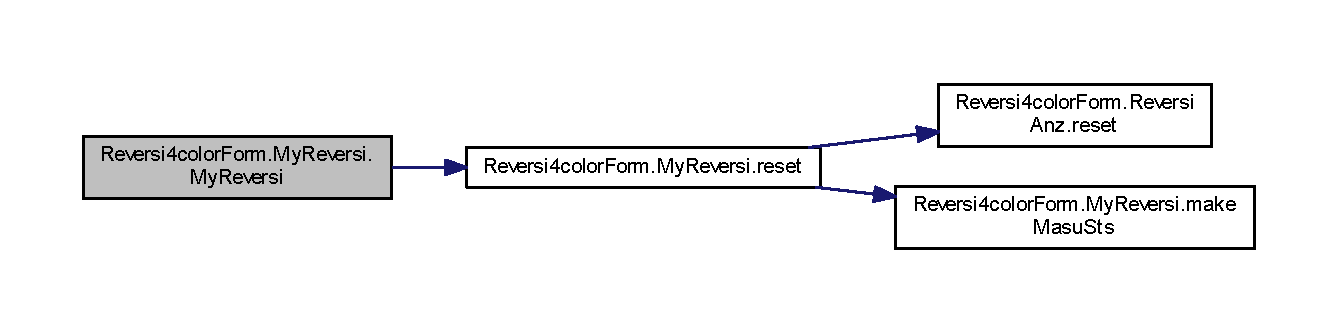
\includegraphics[width=350pt]{class_reversi4color_form_1_1_my_reversi_af58387f6a43abefc531e9098cdb5e08d_cgraph}
\end{center}
\end{figure}


\subsection{Member Function Documentation}
\mbox{\Hypertarget{class_reversi4color_form_1_1_my_reversi_ade9840e10e80b3e908a406efe9ee1372}\label{class_reversi4color_form_1_1_my_reversi_ade9840e10e80b3e908a406efe9ee1372}} 
\index{Reversi4color\+Form\+::\+My\+Reversi@{Reversi4color\+Form\+::\+My\+Reversi}!Analysis\+Reversi@{Analysis\+Reversi}}
\index{Analysis\+Reversi@{Analysis\+Reversi}!Reversi4color\+Form\+::\+My\+Reversi@{Reversi4color\+Form\+::\+My\+Reversi}}
\subsubsection{\texorpdfstring{Analysis\+Reversi()}{AnalysisReversi()}}
{\footnotesize\ttfamily void Reversi4color\+Form.\+My\+Reversi.\+Analysis\+Reversi (\begin{DoxyParamCaption}\item[{int}]{b\+Pass\+Ena,  }\item[{int}]{w\+Pass\+Ena,  }\item[{int}]{l\+Pass\+Ena,  }\item[{int}]{r\+Pass\+Ena }\end{DoxyParamCaption})}



解析を行う 


\begin{DoxyParams}[1]{Parameters}
\mbox{\tt in}  & {\em int} & b\+Pass\+Ena 1=黒パス有効 \\
\hline
\mbox{\tt in}  & {\em int} & w\+Pass\+Ena 1=白パス有効 \\
\hline
\mbox{\tt in}  & {\em int} & l\+Pass\+Ena 1=青パス有効 \\
\hline
\mbox{\tt in}  & {\em int} & r\+Pass\+Ena 1=赤パス有効 \\
\hline
\end{DoxyParams}
\begin{DoxyReturn}{Returns}
ありません 
\end{DoxyReturn}
\begin{DoxyAuthor}{Author}
Yuta Yoshinaga 
\end{DoxyAuthor}
\begin{DoxyDate}{Date}
2017.\+10.\+20 
\end{DoxyDate}


Definition at line 1628 of file My\+Reversi.\+cs.



Referenced by Reversi4color\+Form.\+Reversi\+Play.\+reset(), Reversi4color\+Form.\+Reversi\+Play.\+reversi\+Play(), and Reversi4color\+Form.\+Reversi\+Play.\+reversi\+Play\+Cpu().

Here is the call graph for this function\+:\nopagebreak
\begin{figure}[H]
\begin{center}
\leavevmode
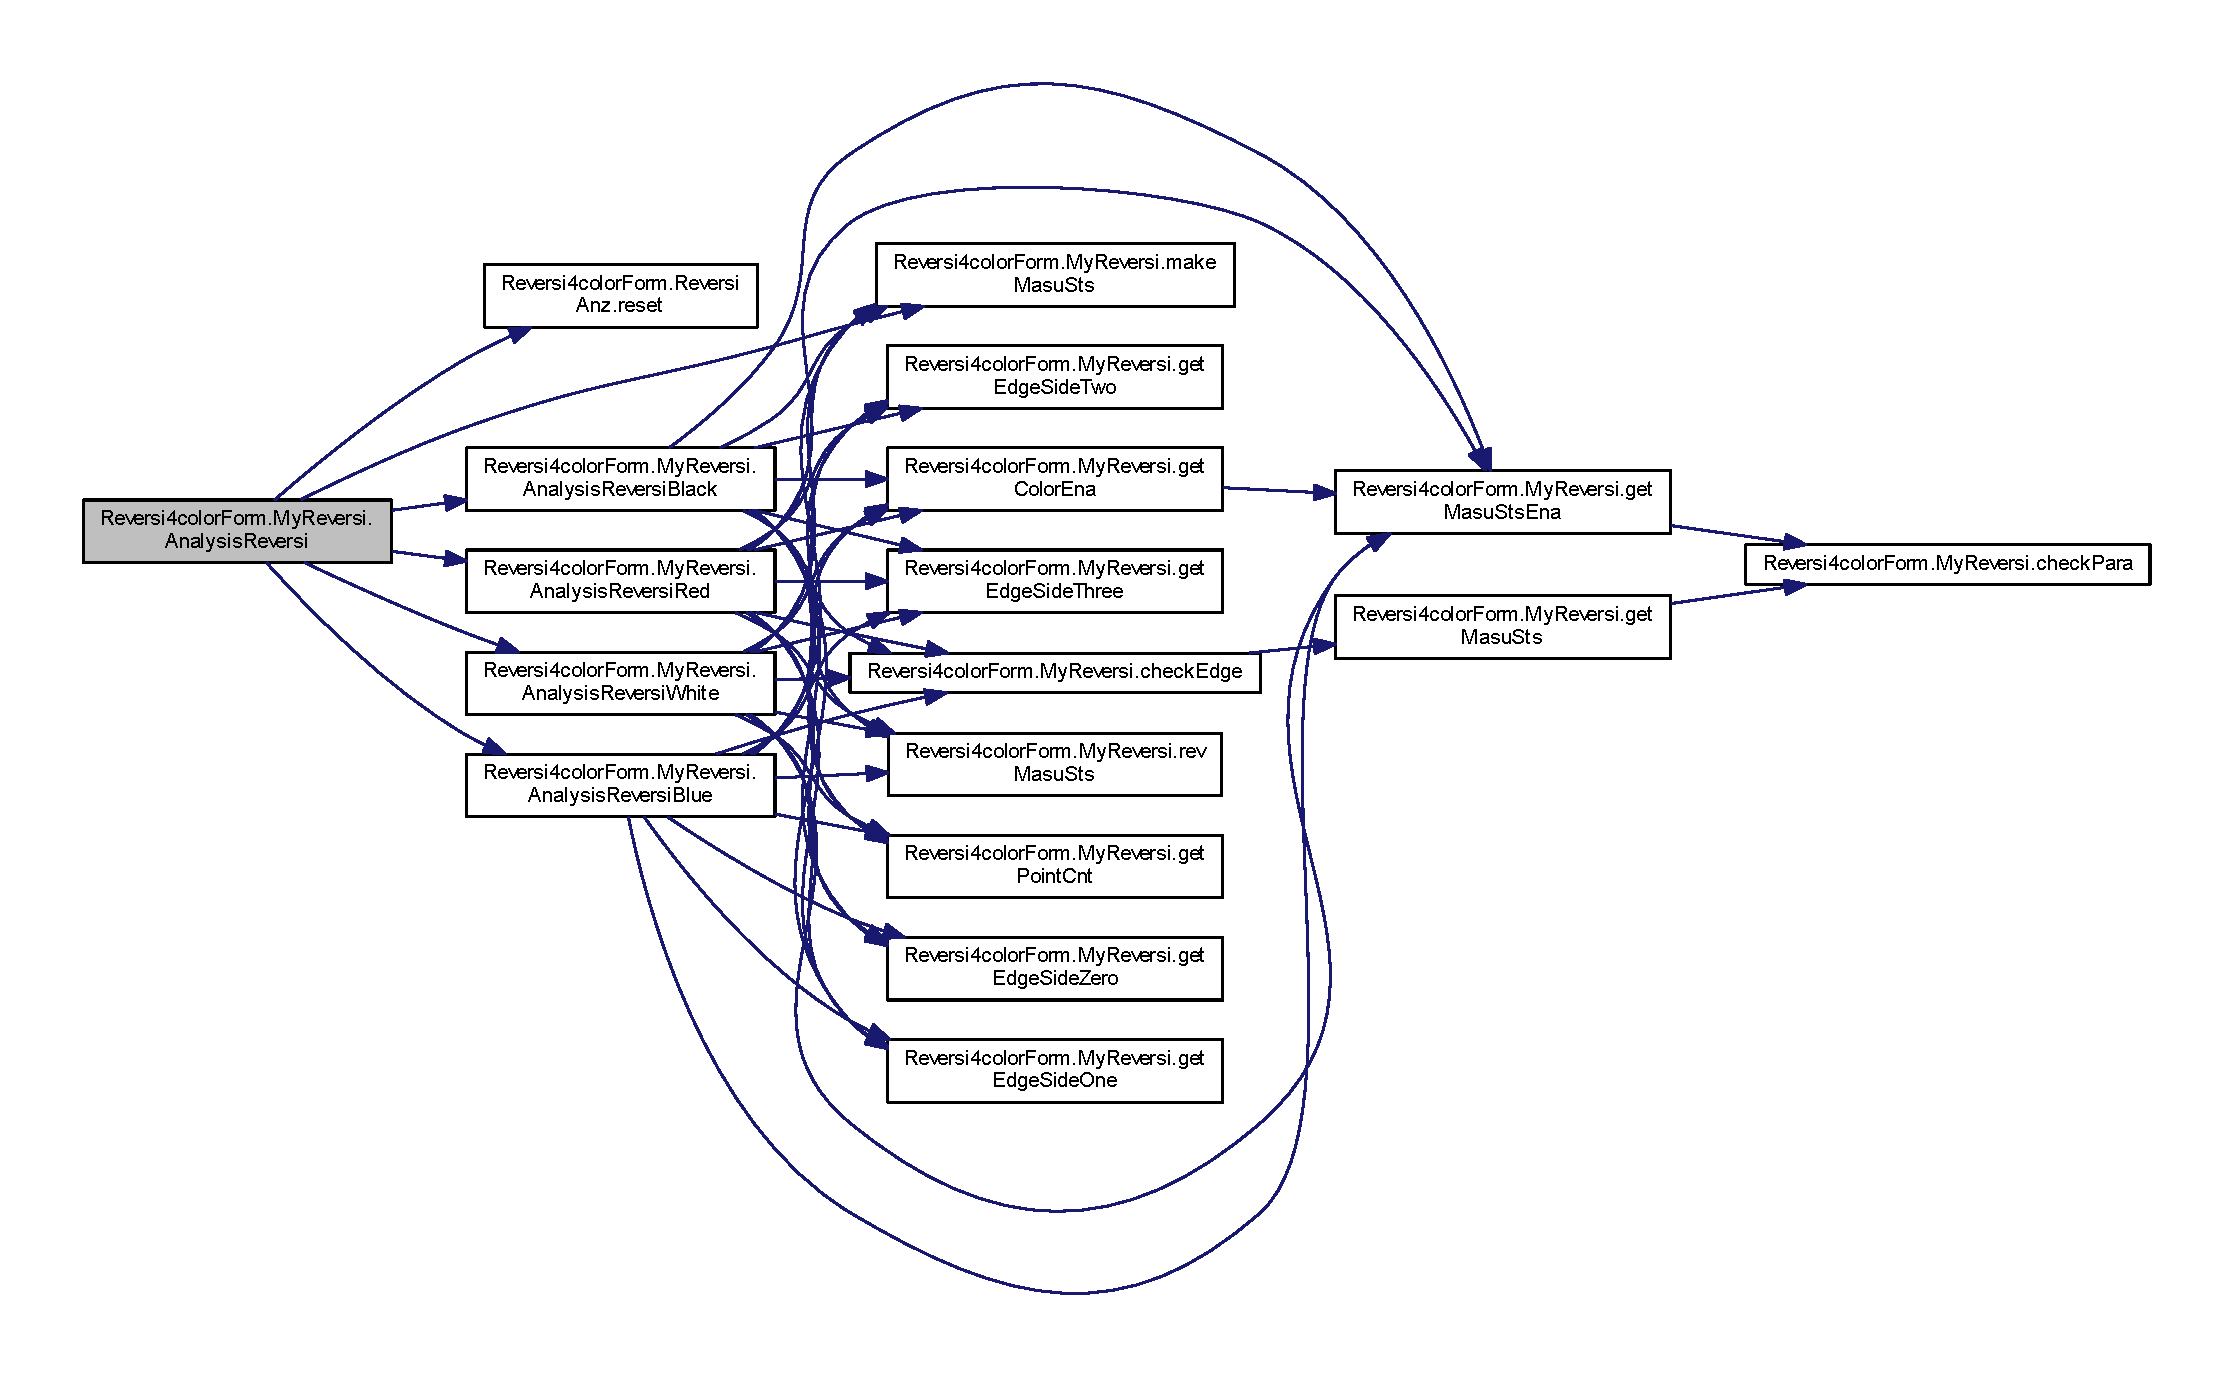
\includegraphics[width=350pt]{class_reversi4color_form_1_1_my_reversi_ade9840e10e80b3e908a406efe9ee1372_cgraph}
\end{center}
\end{figure}
Here is the caller graph for this function\+:\nopagebreak
\begin{figure}[H]
\begin{center}
\leavevmode
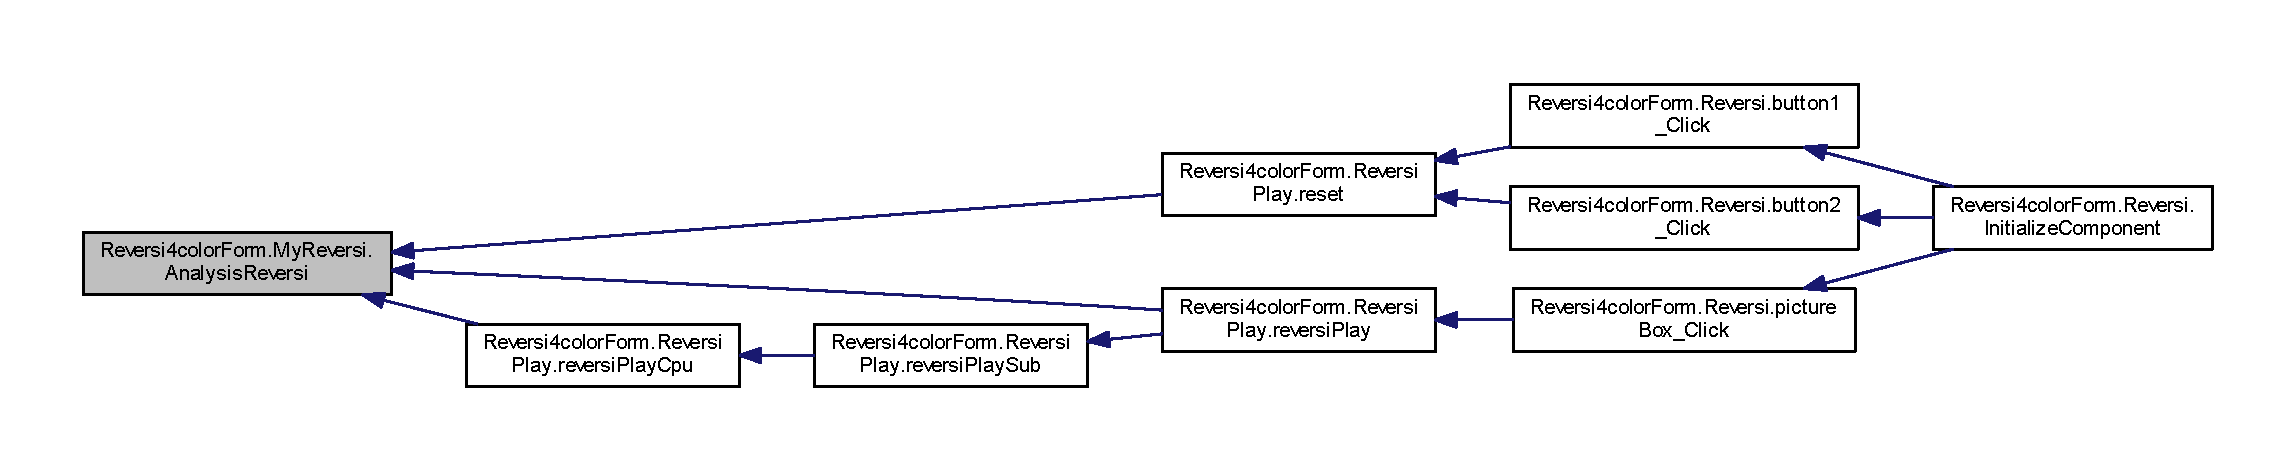
\includegraphics[width=350pt]{class_reversi4color_form_1_1_my_reversi_ade9840e10e80b3e908a406efe9ee1372_icgraph}
\end{center}
\end{figure}
\mbox{\Hypertarget{class_reversi4color_form_1_1_my_reversi_ae4c0b7e9a3cedba827facf1d96b654f0}\label{class_reversi4color_form_1_1_my_reversi_ae4c0b7e9a3cedba827facf1d96b654f0}} 
\index{Reversi4color\+Form\+::\+My\+Reversi@{Reversi4color\+Form\+::\+My\+Reversi}!Analysis\+Reversi\+Black@{Analysis\+Reversi\+Black}}
\index{Analysis\+Reversi\+Black@{Analysis\+Reversi\+Black}!Reversi4color\+Form\+::\+My\+Reversi@{Reversi4color\+Form\+::\+My\+Reversi}}
\subsubsection{\texorpdfstring{Analysis\+Reversi\+Black()}{AnalysisReversiBlack()}}
{\footnotesize\ttfamily void Reversi4color\+Form.\+My\+Reversi.\+Analysis\+Reversi\+Black (\begin{DoxyParamCaption}{ }\end{DoxyParamCaption})\hspace{0.3cm}{\ttfamily [private]}}



解析を行う(黒) 

\begin{DoxyReturn}{Returns}
ありません 
\end{DoxyReturn}
\begin{DoxyAuthor}{Author}
Yuta Yoshinaga 
\end{DoxyAuthor}
\begin{DoxyDate}{Date}
2017.\+10.\+20 
\end{DoxyDate}


Definition at line 848 of file My\+Reversi.\+cs.



Referenced by Reversi4color\+Form.\+My\+Reversi.\+Analysis\+Reversi().

Here is the call graph for this function\+:\nopagebreak
\begin{figure}[H]
\begin{center}
\leavevmode
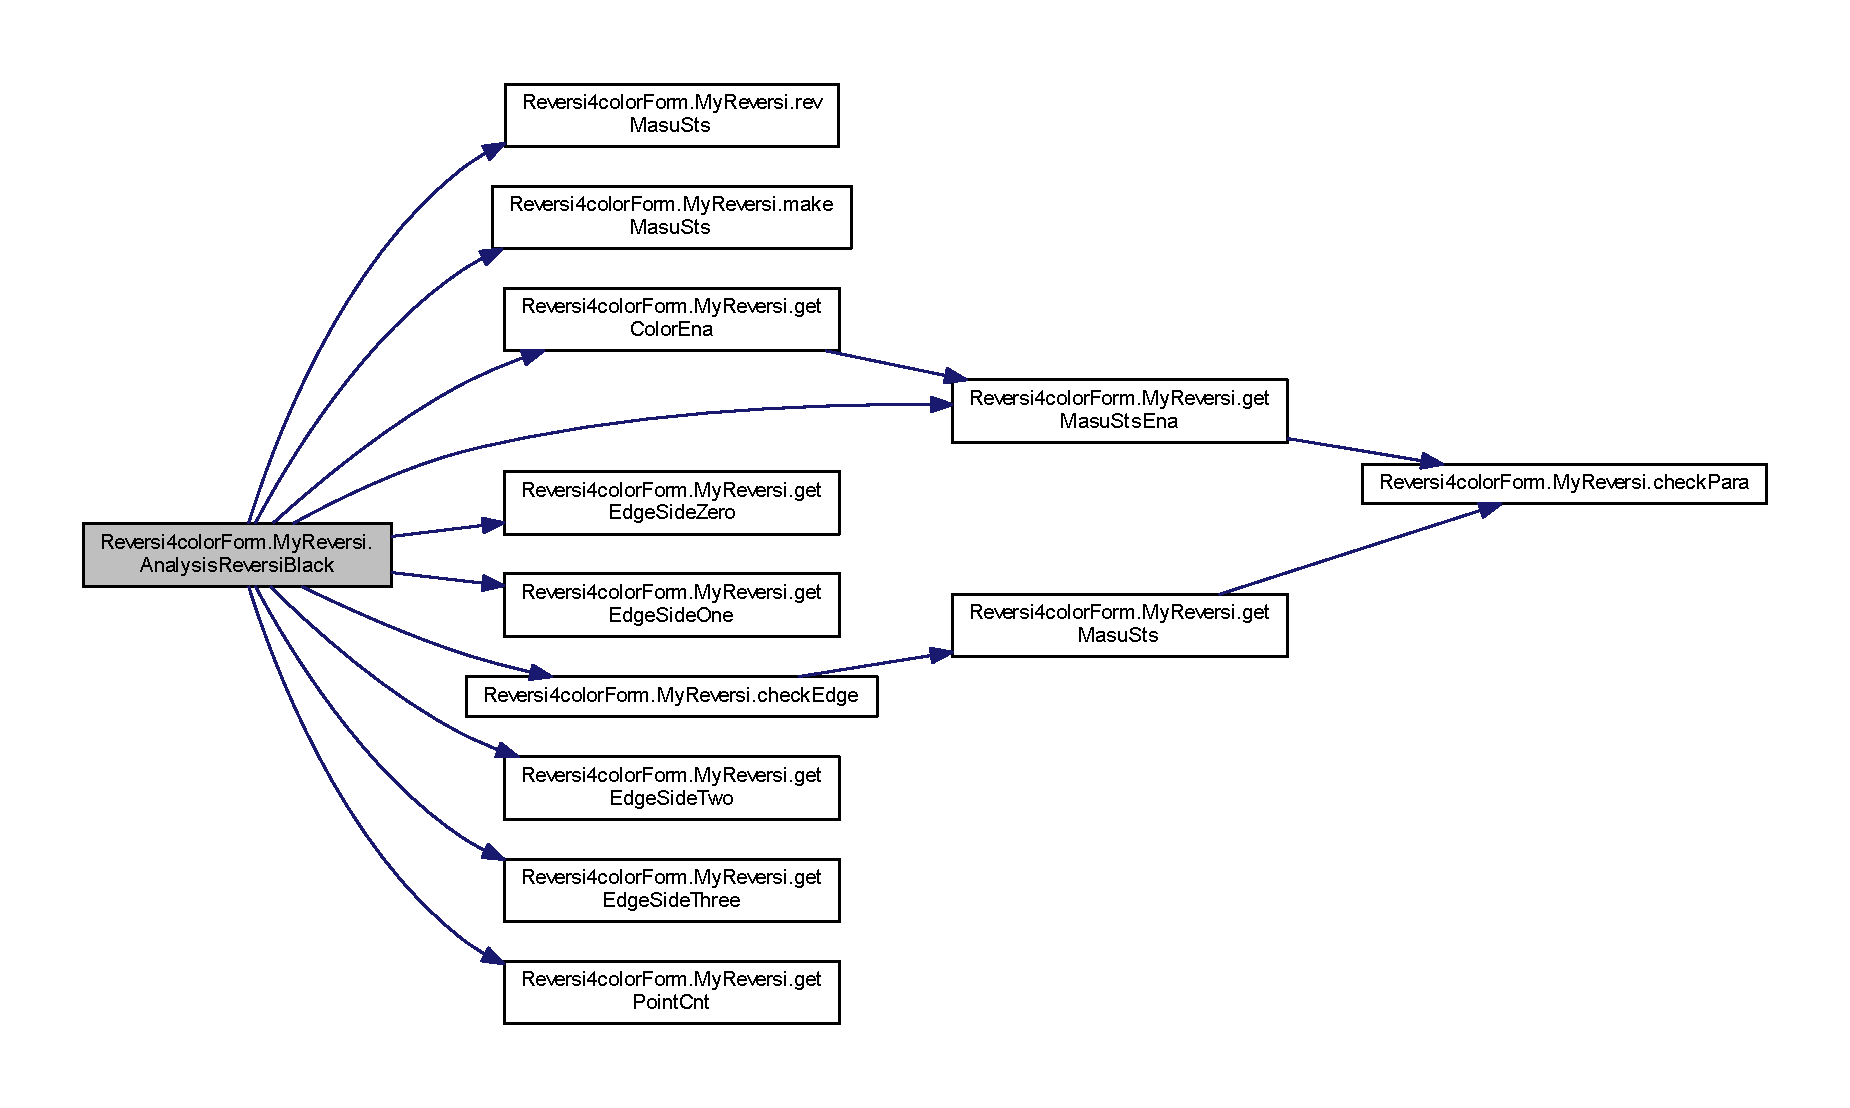
\includegraphics[width=350pt]{class_reversi4color_form_1_1_my_reversi_ae4c0b7e9a3cedba827facf1d96b654f0_cgraph}
\end{center}
\end{figure}
Here is the caller graph for this function\+:\nopagebreak
\begin{figure}[H]
\begin{center}
\leavevmode
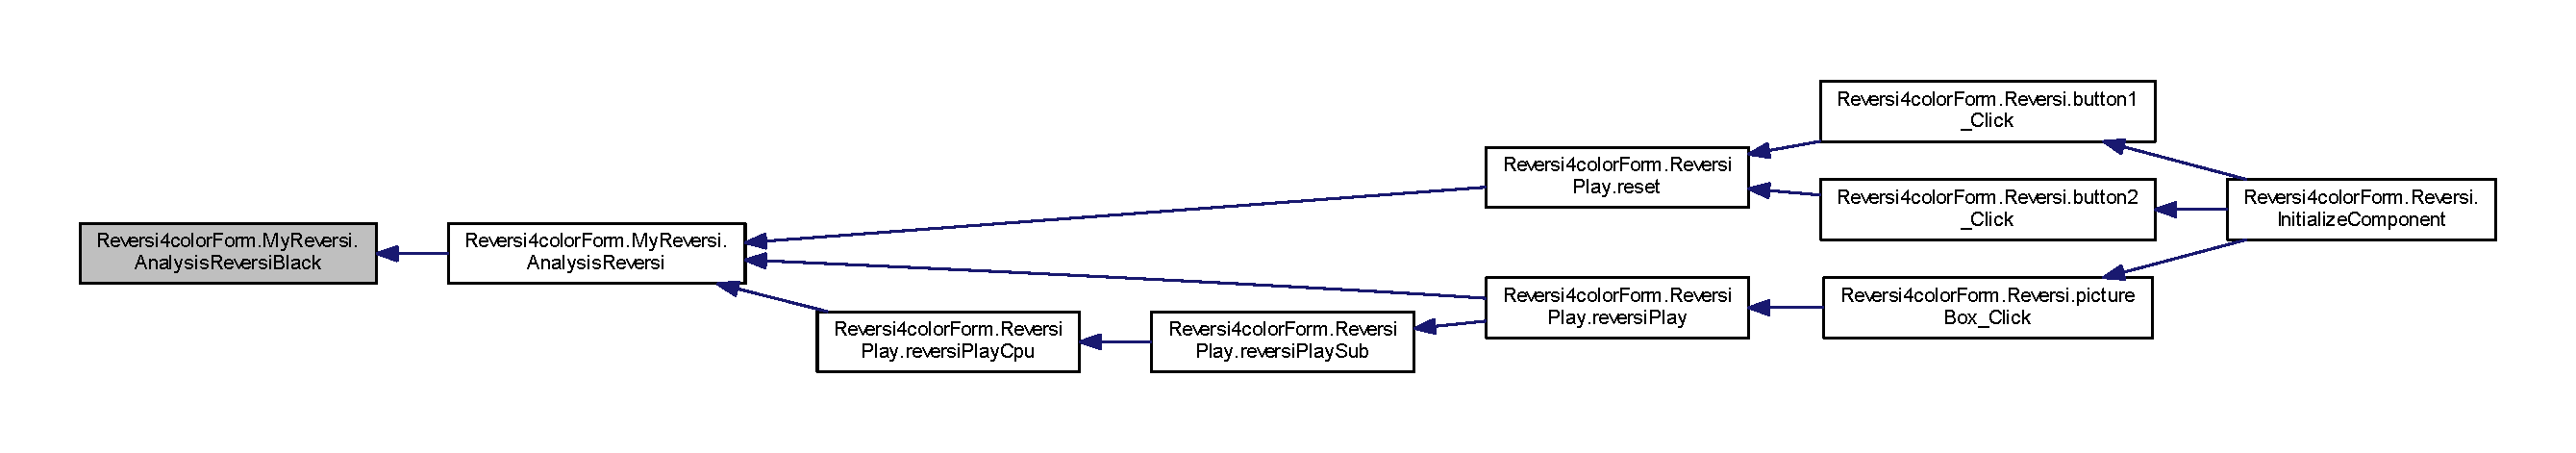
\includegraphics[width=350pt]{class_reversi4color_form_1_1_my_reversi_ae4c0b7e9a3cedba827facf1d96b654f0_icgraph}
\end{center}
\end{figure}
\mbox{\Hypertarget{class_reversi4color_form_1_1_my_reversi_a07c18a7adbcc3bd0993673f0a8f63c85}\label{class_reversi4color_form_1_1_my_reversi_a07c18a7adbcc3bd0993673f0a8f63c85}} 
\index{Reversi4color\+Form\+::\+My\+Reversi@{Reversi4color\+Form\+::\+My\+Reversi}!Analysis\+Reversi\+Blue@{Analysis\+Reversi\+Blue}}
\index{Analysis\+Reversi\+Blue@{Analysis\+Reversi\+Blue}!Reversi4color\+Form\+::\+My\+Reversi@{Reversi4color\+Form\+::\+My\+Reversi}}
\subsubsection{\texorpdfstring{Analysis\+Reversi\+Blue()}{AnalysisReversiBlue()}}
{\footnotesize\ttfamily void Reversi4color\+Form.\+My\+Reversi.\+Analysis\+Reversi\+Blue (\begin{DoxyParamCaption}{ }\end{DoxyParamCaption})\hspace{0.3cm}{\ttfamily [private]}}



解析を行う(青) 

\begin{DoxyReturn}{Returns}
ありません 
\end{DoxyReturn}
\begin{DoxyAuthor}{Author}
Yuta Yoshinaga 
\end{DoxyAuthor}
\begin{DoxyDate}{Date}
2017.\+10.\+20 
\end{DoxyDate}


Definition at line 1234 of file My\+Reversi.\+cs.



Referenced by Reversi4color\+Form.\+My\+Reversi.\+Analysis\+Reversi().

Here is the call graph for this function\+:\nopagebreak
\begin{figure}[H]
\begin{center}
\leavevmode
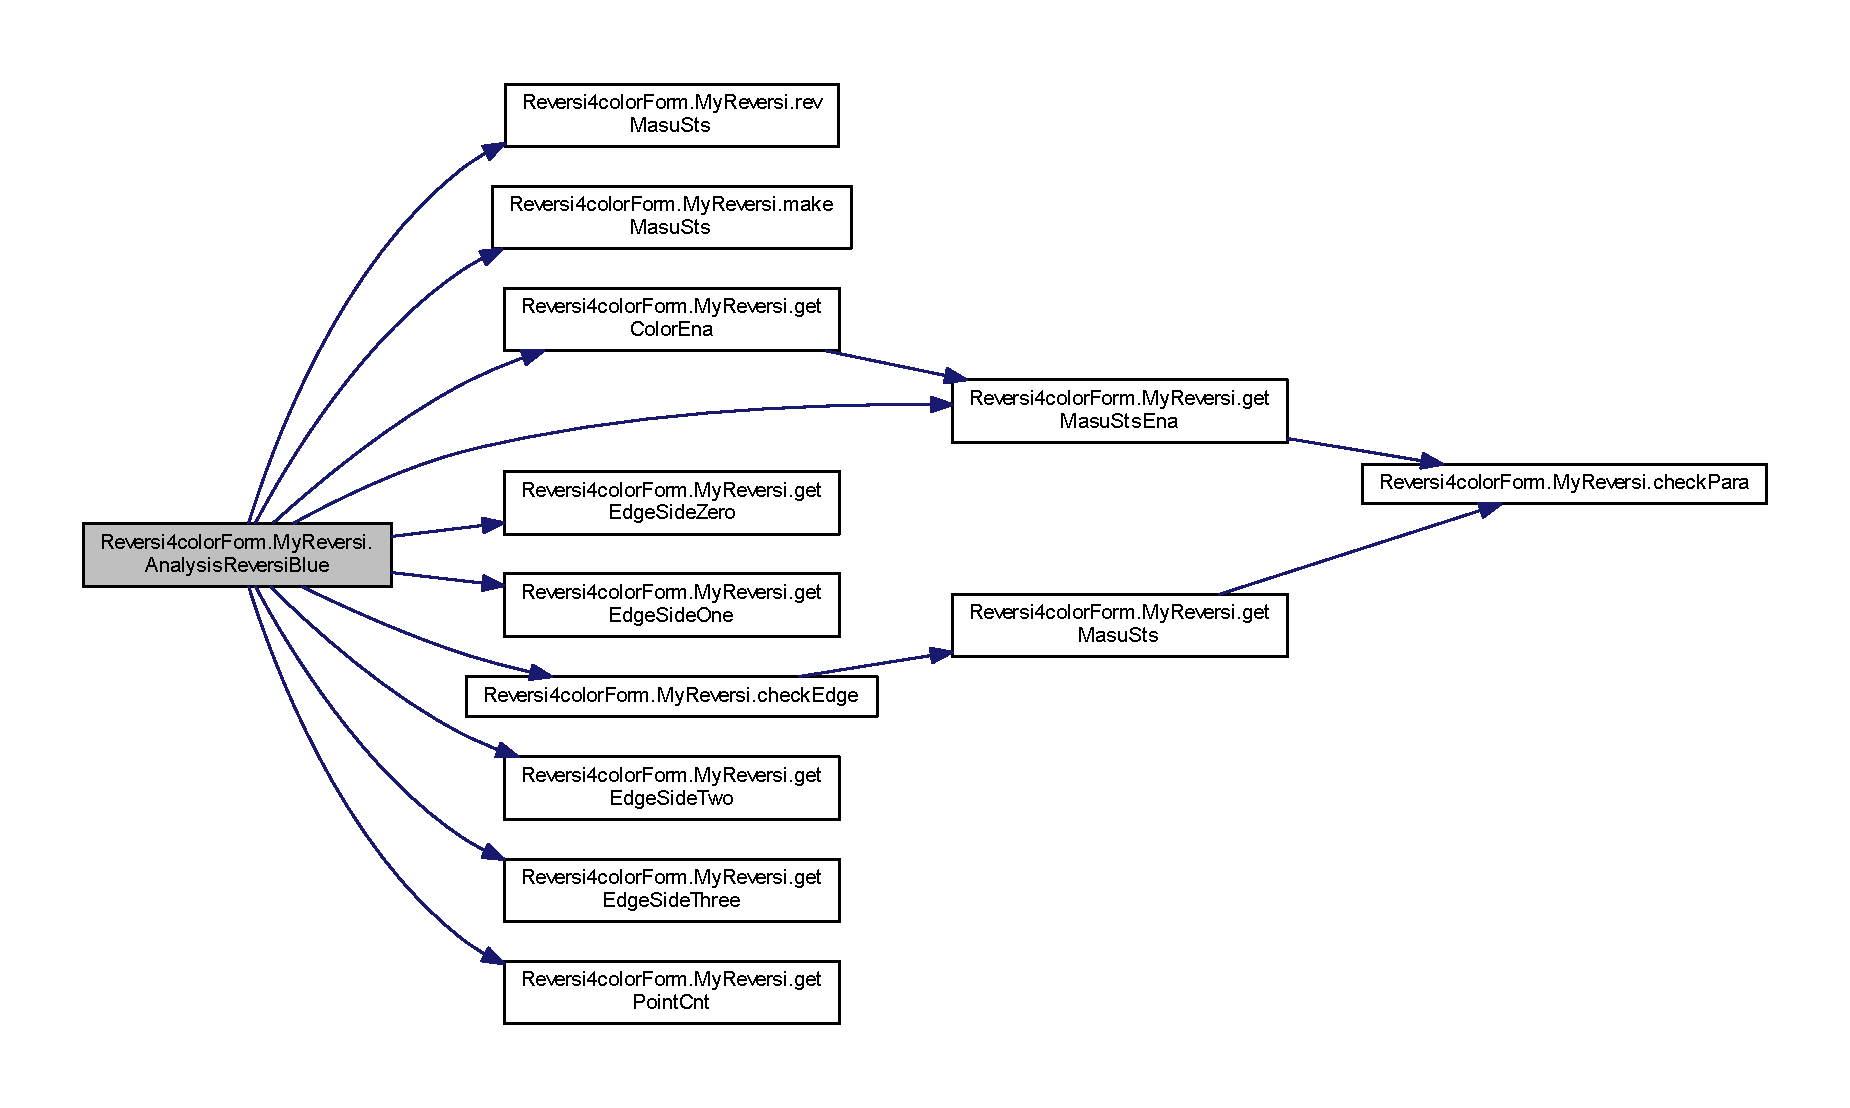
\includegraphics[width=350pt]{class_reversi4color_form_1_1_my_reversi_a07c18a7adbcc3bd0993673f0a8f63c85_cgraph}
\end{center}
\end{figure}
Here is the caller graph for this function\+:\nopagebreak
\begin{figure}[H]
\begin{center}
\leavevmode
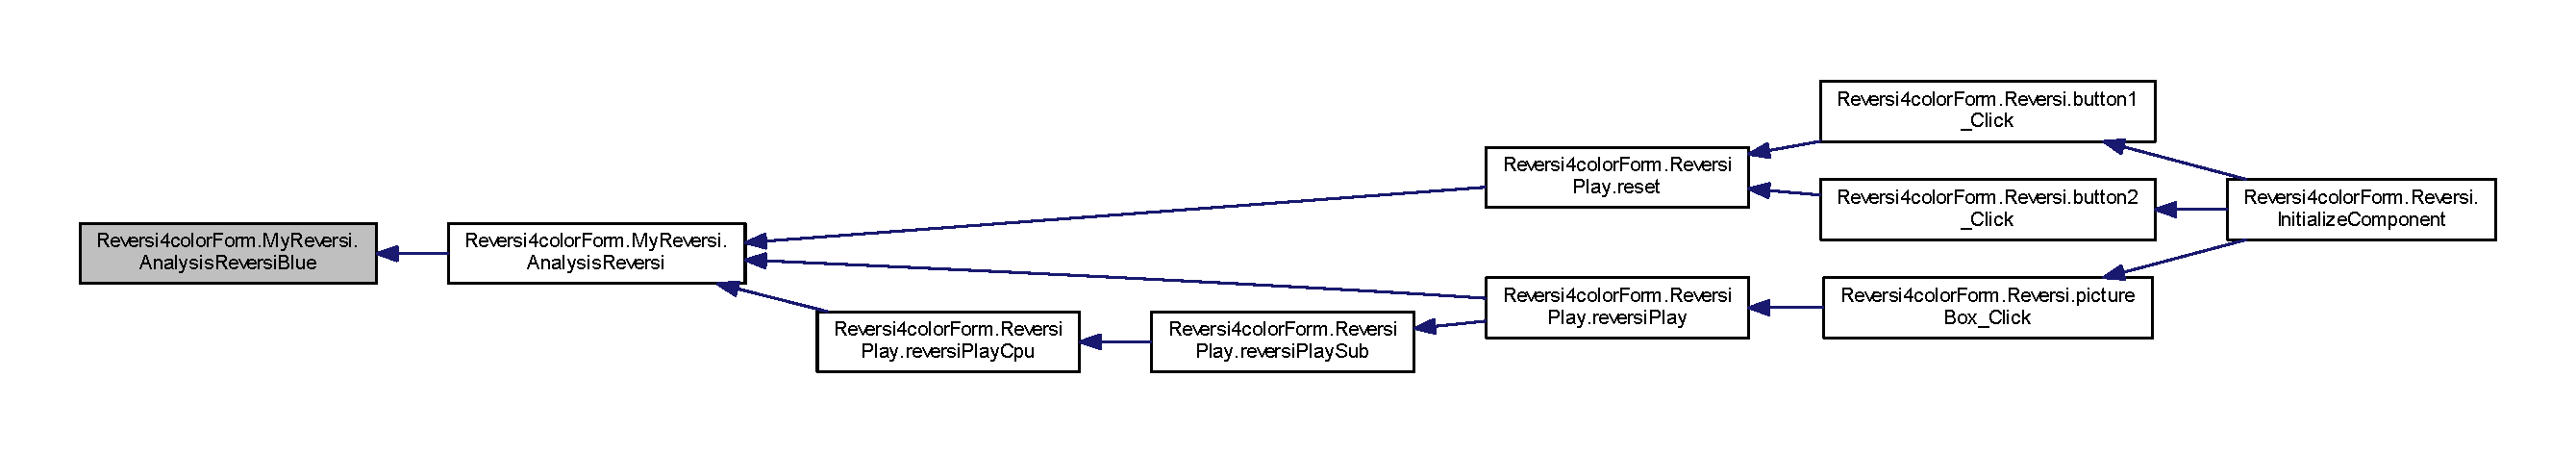
\includegraphics[width=350pt]{class_reversi4color_form_1_1_my_reversi_a07c18a7adbcc3bd0993673f0a8f63c85_icgraph}
\end{center}
\end{figure}
\mbox{\Hypertarget{class_reversi4color_form_1_1_my_reversi_a2d0c12ed7036def583e06ca4df37f367}\label{class_reversi4color_form_1_1_my_reversi_a2d0c12ed7036def583e06ca4df37f367}} 
\index{Reversi4color\+Form\+::\+My\+Reversi@{Reversi4color\+Form\+::\+My\+Reversi}!Analysis\+Reversi\+Red@{Analysis\+Reversi\+Red}}
\index{Analysis\+Reversi\+Red@{Analysis\+Reversi\+Red}!Reversi4color\+Form\+::\+My\+Reversi@{Reversi4color\+Form\+::\+My\+Reversi}}
\subsubsection{\texorpdfstring{Analysis\+Reversi\+Red()}{AnalysisReversiRed()}}
{\footnotesize\ttfamily void Reversi4color\+Form.\+My\+Reversi.\+Analysis\+Reversi\+Red (\begin{DoxyParamCaption}{ }\end{DoxyParamCaption})\hspace{0.3cm}{\ttfamily [private]}}



解析を行う(赤) 

\begin{DoxyReturn}{Returns}
ありません 
\end{DoxyReturn}
\begin{DoxyAuthor}{Author}
Yuta Yoshinaga 
\end{DoxyAuthor}
\begin{DoxyDate}{Date}
2017.\+10.\+20 
\end{DoxyDate}


Definition at line 1429 of file My\+Reversi.\+cs.



Referenced by Reversi4color\+Form.\+My\+Reversi.\+Analysis\+Reversi().

Here is the call graph for this function\+:\nopagebreak
\begin{figure}[H]
\begin{center}
\leavevmode
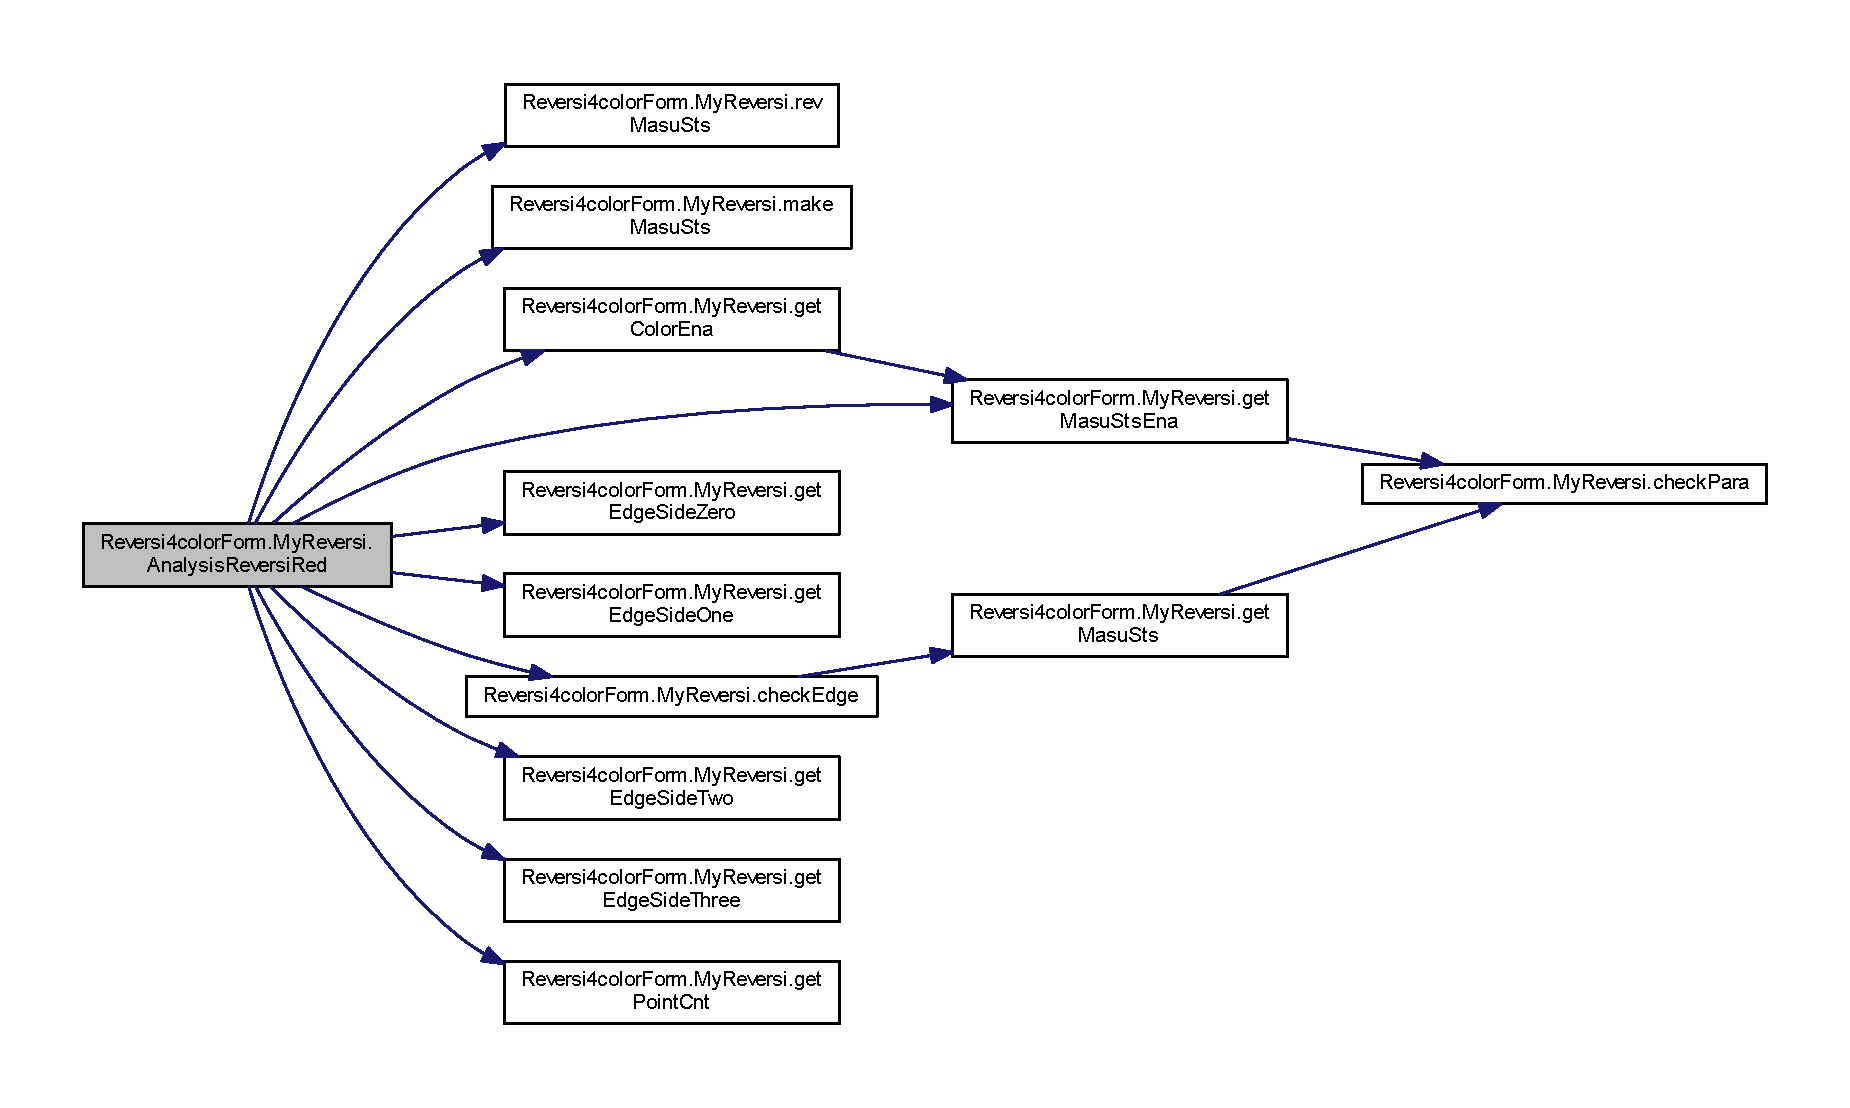
\includegraphics[width=350pt]{class_reversi4color_form_1_1_my_reversi_a2d0c12ed7036def583e06ca4df37f367_cgraph}
\end{center}
\end{figure}
Here is the caller graph for this function\+:\nopagebreak
\begin{figure}[H]
\begin{center}
\leavevmode
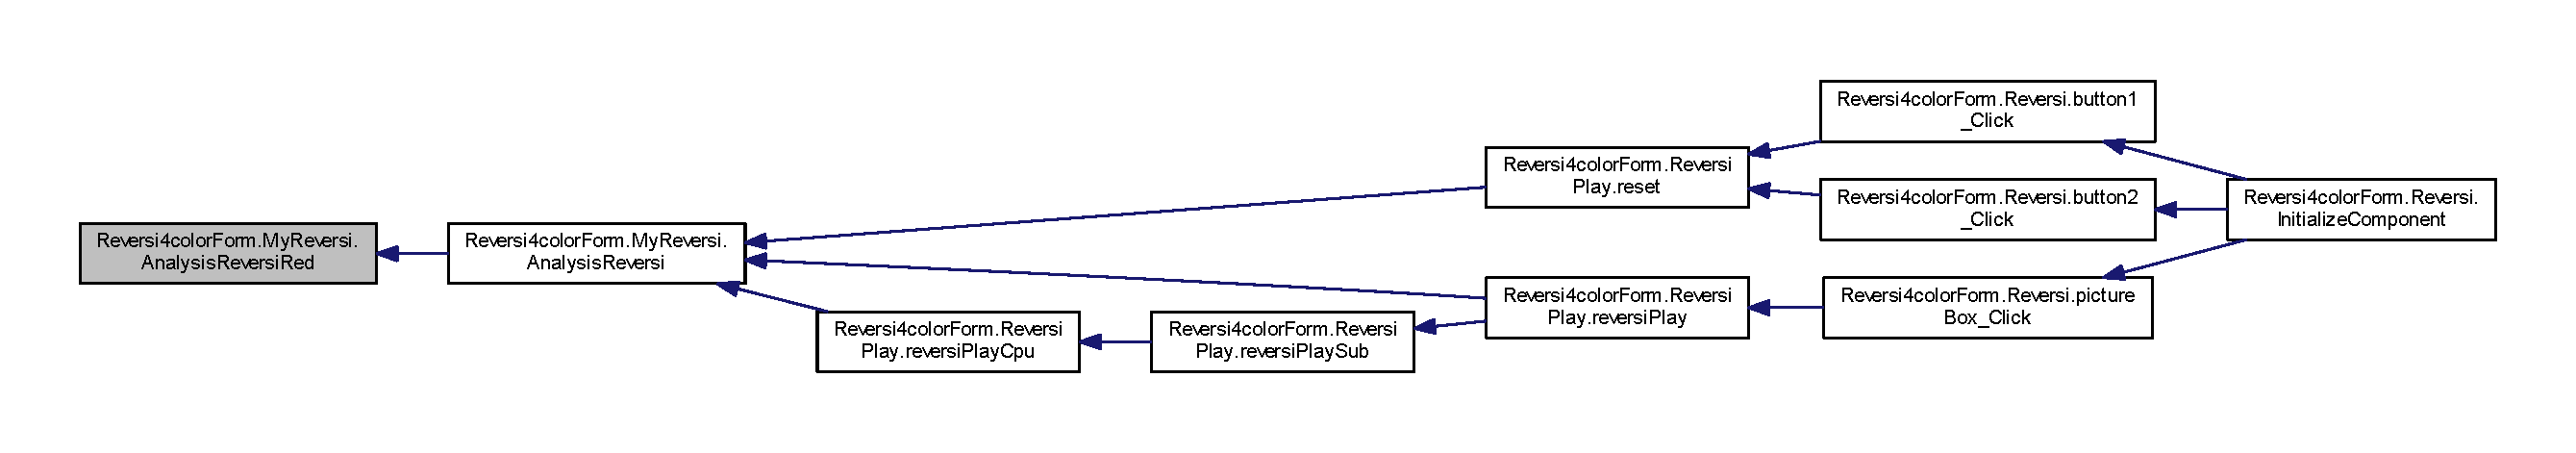
\includegraphics[width=350pt]{class_reversi4color_form_1_1_my_reversi_a2d0c12ed7036def583e06ca4df37f367_icgraph}
\end{center}
\end{figure}
\mbox{\Hypertarget{class_reversi4color_form_1_1_my_reversi_a61ca891ff78c7357ab077ce7bd3cbf97}\label{class_reversi4color_form_1_1_my_reversi_a61ca891ff78c7357ab077ce7bd3cbf97}} 
\index{Reversi4color\+Form\+::\+My\+Reversi@{Reversi4color\+Form\+::\+My\+Reversi}!Analysis\+Reversi\+White@{Analysis\+Reversi\+White}}
\index{Analysis\+Reversi\+White@{Analysis\+Reversi\+White}!Reversi4color\+Form\+::\+My\+Reversi@{Reversi4color\+Form\+::\+My\+Reversi}}
\subsubsection{\texorpdfstring{Analysis\+Reversi\+White()}{AnalysisReversiWhite()}}
{\footnotesize\ttfamily void Reversi4color\+Form.\+My\+Reversi.\+Analysis\+Reversi\+White (\begin{DoxyParamCaption}{ }\end{DoxyParamCaption})\hspace{0.3cm}{\ttfamily [private]}}



解析を行う(白) 

\begin{DoxyReturn}{Returns}
ありません 
\end{DoxyReturn}
\begin{DoxyAuthor}{Author}
Yuta Yoshinaga 
\end{DoxyAuthor}
\begin{DoxyDate}{Date}
2017.\+10.\+20 
\end{DoxyDate}


Definition at line 1041 of file My\+Reversi.\+cs.



Referenced by Reversi4color\+Form.\+My\+Reversi.\+Analysis\+Reversi().

Here is the call graph for this function\+:\nopagebreak
\begin{figure}[H]
\begin{center}
\leavevmode
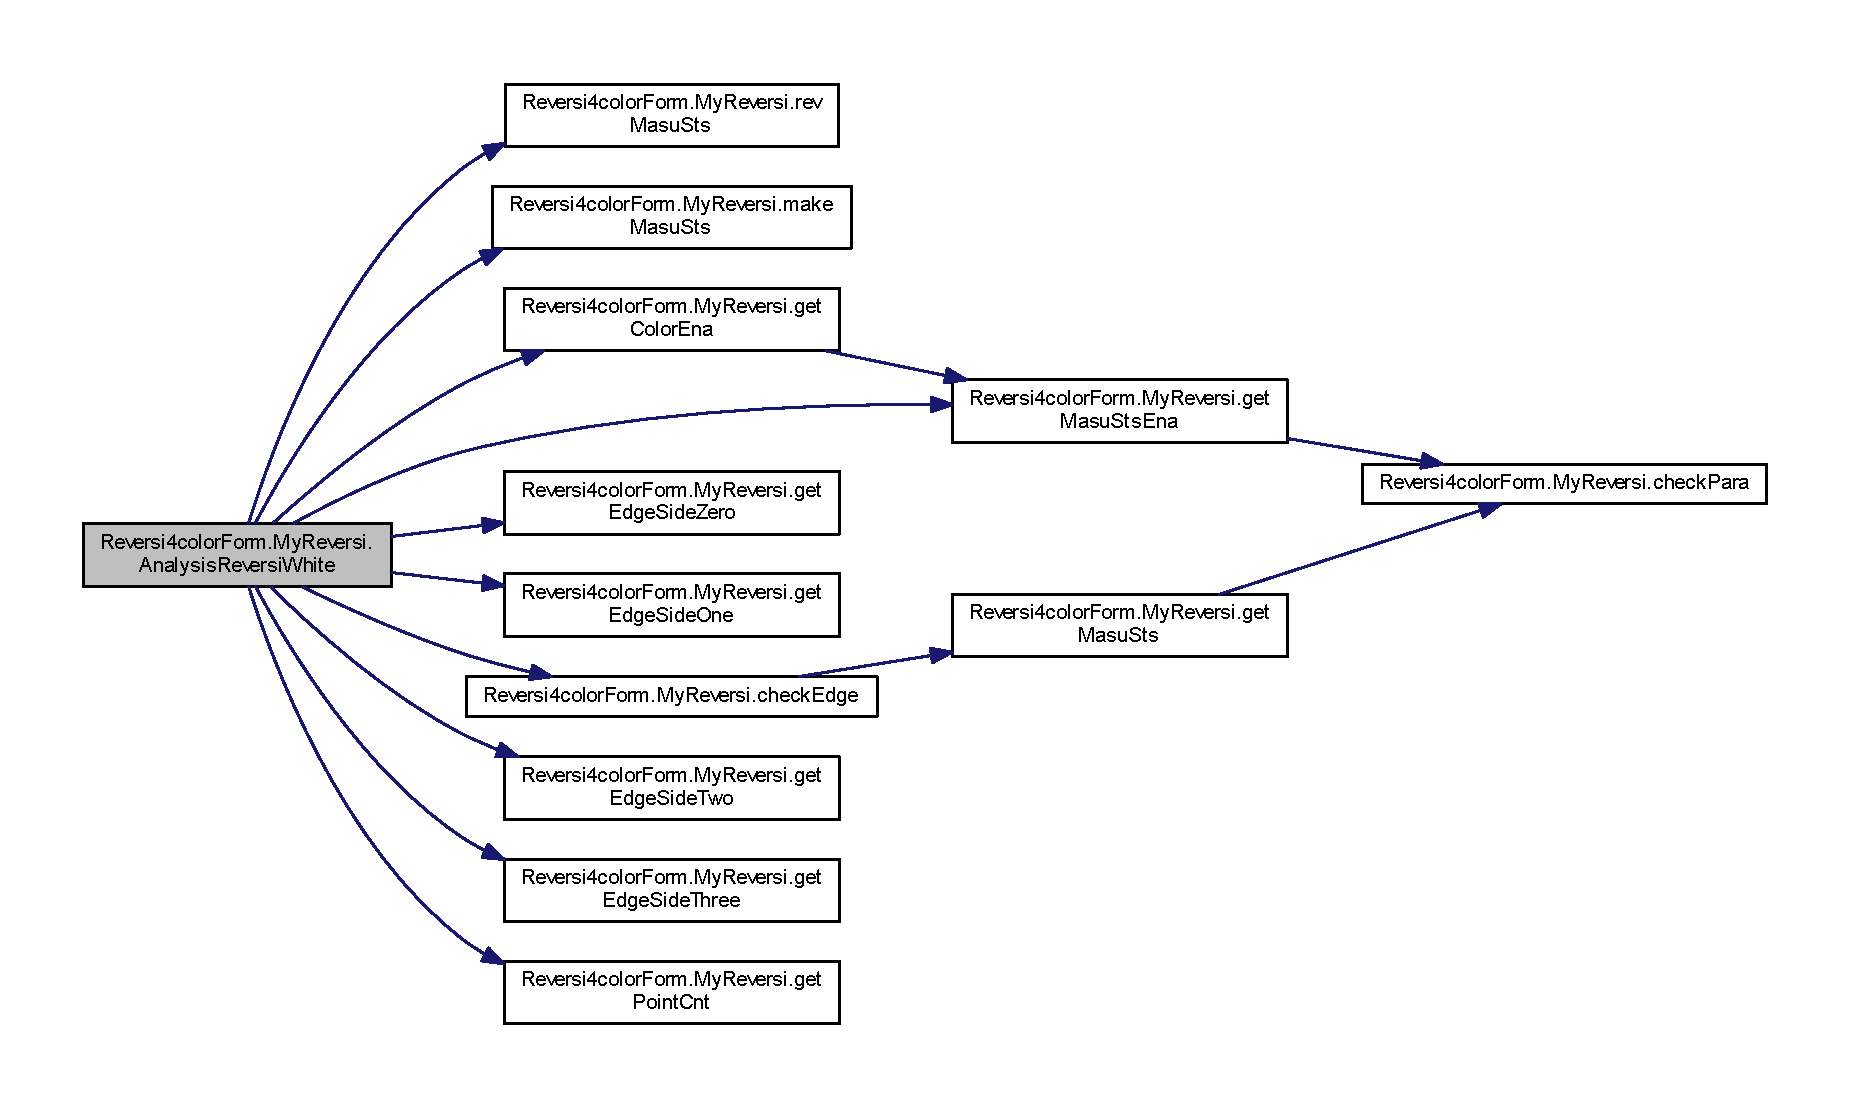
\includegraphics[width=350pt]{class_reversi4color_form_1_1_my_reversi_a61ca891ff78c7357ab077ce7bd3cbf97_cgraph}
\end{center}
\end{figure}
Here is the caller graph for this function\+:\nopagebreak
\begin{figure}[H]
\begin{center}
\leavevmode
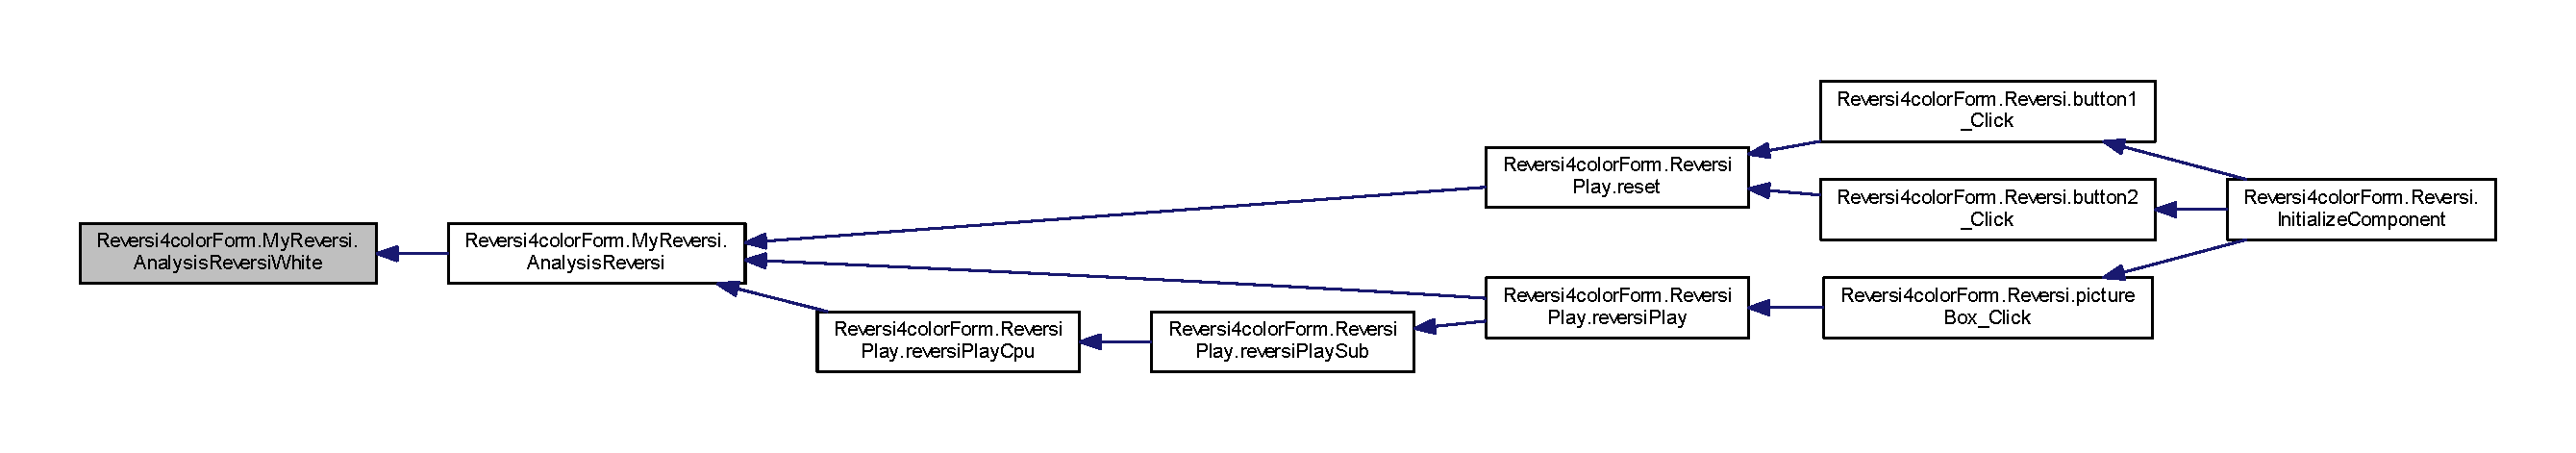
\includegraphics[width=350pt]{class_reversi4color_form_1_1_my_reversi_a61ca891ff78c7357ab077ce7bd3cbf97_icgraph}
\end{center}
\end{figure}
\mbox{\Hypertarget{class_reversi4color_form_1_1_my_reversi_a8538a52d715eb754c49fc5719390d035}\label{class_reversi4color_form_1_1_my_reversi_a8538a52d715eb754c49fc5719390d035}} 
\index{Reversi4color\+Form\+::\+My\+Reversi@{Reversi4color\+Form\+::\+My\+Reversi}!check\+Edge@{check\+Edge}}
\index{check\+Edge@{check\+Edge}!Reversi4color\+Form\+::\+My\+Reversi@{Reversi4color\+Form\+::\+My\+Reversi}}
\subsubsection{\texorpdfstring{check\+Edge()}{checkEdge()}}
{\footnotesize\ttfamily int Reversi4color\+Form.\+My\+Reversi.\+check\+Edge (\begin{DoxyParamCaption}\item[{int}]{color,  }\item[{int}]{y,  }\item[{int}]{x }\end{DoxyParamCaption})}



角の隣に置いても角を取られないマス検索 


\begin{DoxyParams}[1]{Parameters}
\mbox{\tt in}  & {\em int} & color コマ色 \\
\hline
\mbox{\tt in}  & {\em int} & y マスの\+Y座標 \\
\hline
\mbox{\tt in}  & {\em int} & x マスの\+X座標 \\
\hline
\end{DoxyParams}
\begin{DoxyReturn}{Returns}
0 \+: 取られる それ以外 \+: 取られない 
\end{DoxyReturn}
\begin{DoxyAuthor}{Author}
Yuta Yoshinaga 
\end{DoxyAuthor}
\begin{DoxyDate}{Date}
2017.\+10.\+20 
\end{DoxyDate}


Definition at line 2024 of file My\+Reversi.\+cs.



Referenced by Reversi4color\+Form.\+My\+Reversi.\+Analysis\+Reversi\+Black(), Reversi4color\+Form.\+My\+Reversi.\+Analysis\+Reversi\+Blue(), Reversi4color\+Form.\+My\+Reversi.\+Analysis\+Reversi\+Red(), Reversi4color\+Form.\+My\+Reversi.\+Analysis\+Reversi\+White(), and Reversi4color\+Form.\+Reversi\+Play.\+reversi\+Play\+Cpu().

Here is the call graph for this function\+:\nopagebreak
\begin{figure}[H]
\begin{center}
\leavevmode
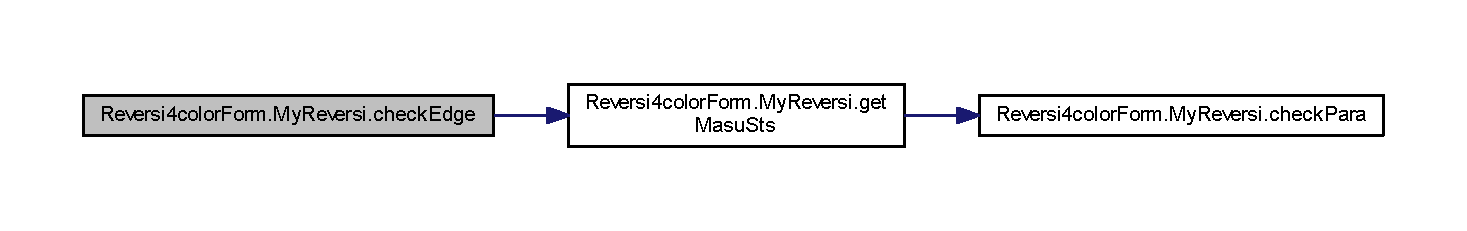
\includegraphics[width=350pt]{class_reversi4color_form_1_1_my_reversi_a8538a52d715eb754c49fc5719390d035_cgraph}
\end{center}
\end{figure}
Here is the caller graph for this function\+:\nopagebreak
\begin{figure}[H]
\begin{center}
\leavevmode
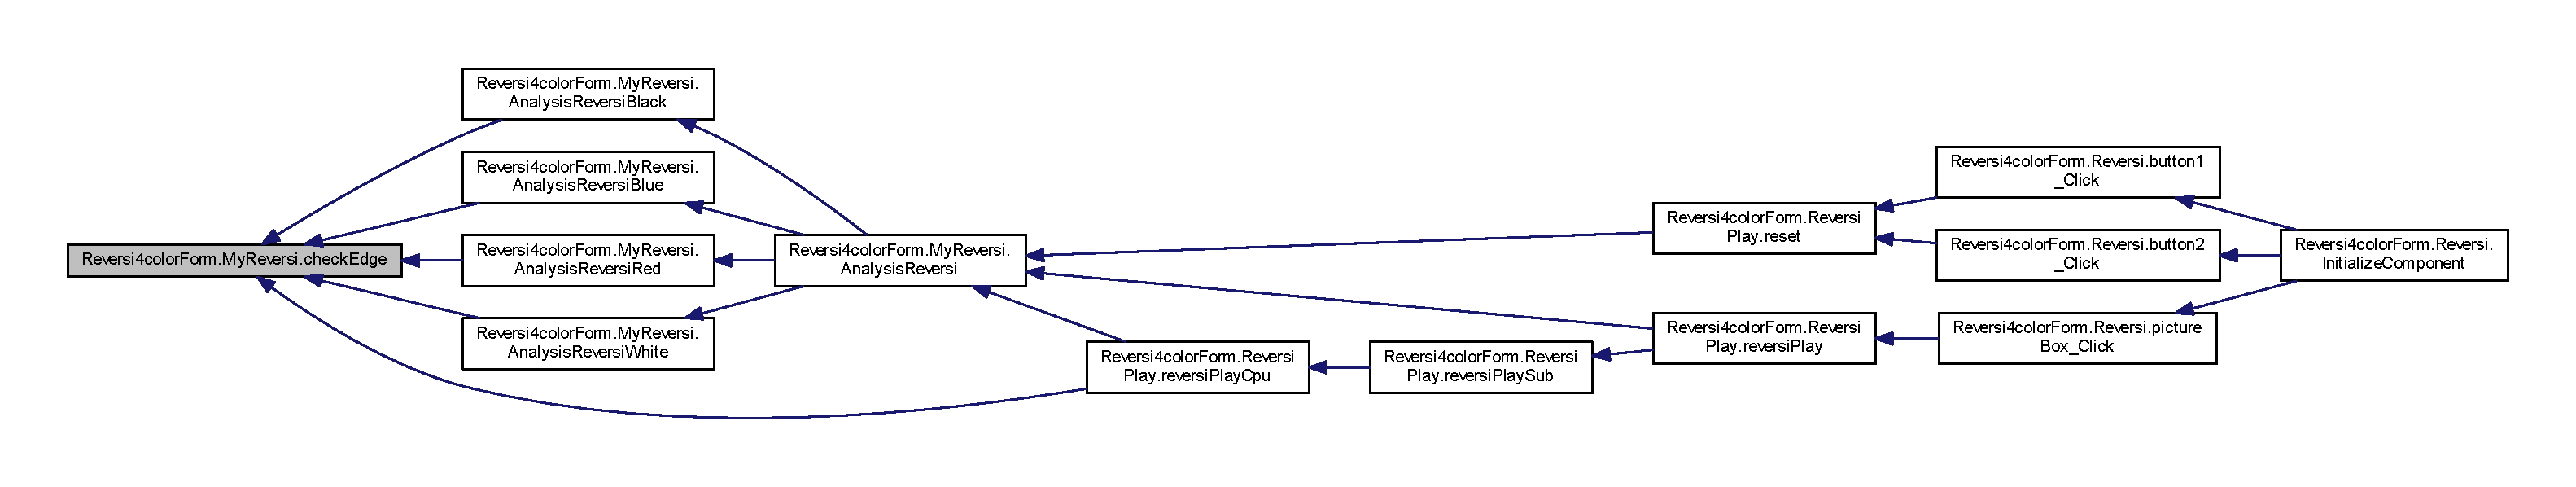
\includegraphics[width=350pt]{class_reversi4color_form_1_1_my_reversi_a8538a52d715eb754c49fc5719390d035_icgraph}
\end{center}
\end{figure}
\mbox{\Hypertarget{class_reversi4color_form_1_1_my_reversi_a02c145ac89302f2360cdb0c0391a38ce}\label{class_reversi4color_form_1_1_my_reversi_a02c145ac89302f2360cdb0c0391a38ce}} 
\index{Reversi4color\+Form\+::\+My\+Reversi@{Reversi4color\+Form\+::\+My\+Reversi}!check\+Para@{check\+Para}}
\index{check\+Para@{check\+Para}!Reversi4color\+Form\+::\+My\+Reversi@{Reversi4color\+Form\+::\+My\+Reversi}}
\subsubsection{\texorpdfstring{check\+Para()}{checkPara()}}
{\footnotesize\ttfamily int Reversi4color\+Form.\+My\+Reversi.\+check\+Para (\begin{DoxyParamCaption}\item[{int}]{para,  }\item[{int}]{min,  }\item[{int}]{max }\end{DoxyParamCaption})\hspace{0.3cm}{\ttfamily [private]}}



パラメーター範囲チェック 


\begin{DoxyParams}[1]{Parameters}
\mbox{\tt in}  & {\em int} & para チェックパラメーター \\
\hline
\mbox{\tt in}  & {\em int} & min パラメーター最小値 \\
\hline
\mbox{\tt in}  & {\em int} & max パラメーター最大値 \\
\hline
\end{DoxyParams}
\begin{DoxyReturn}{Returns}
0 \+: 成功 それ以外 \+: 失敗 
\end{DoxyReturn}
\begin{DoxyAuthor}{Author}
Yuta Yoshinaga 
\end{DoxyAuthor}
\begin{DoxyDate}{Date}
2017.\+10.\+20 
\end{DoxyDate}


Definition at line 833 of file My\+Reversi.\+cs.



Referenced by Reversi4color\+Form.\+My\+Reversi.\+get\+History(), Reversi4color\+Form.\+My\+Reversi.\+get\+Masu\+Sts(), Reversi4color\+Form.\+My\+Reversi.\+get\+Masu\+Sts\+Cnt(), Reversi4color\+Form.\+My\+Reversi.\+get\+Masu\+Sts\+Ena(), Reversi4color\+Form.\+My\+Reversi.\+get\+Masu\+Sts\+Old(), Reversi4color\+Form.\+My\+Reversi.\+get\+Pass\+Ena(), Reversi4color\+Form.\+My\+Reversi.\+get\+Point(), Reversi4color\+Form.\+My\+Reversi.\+get\+Point\+Anz(), and Reversi4color\+Form.\+My\+Reversi.\+set\+Masu\+Cnt().

Here is the caller graph for this function\+:\nopagebreak
\begin{figure}[H]
\begin{center}
\leavevmode
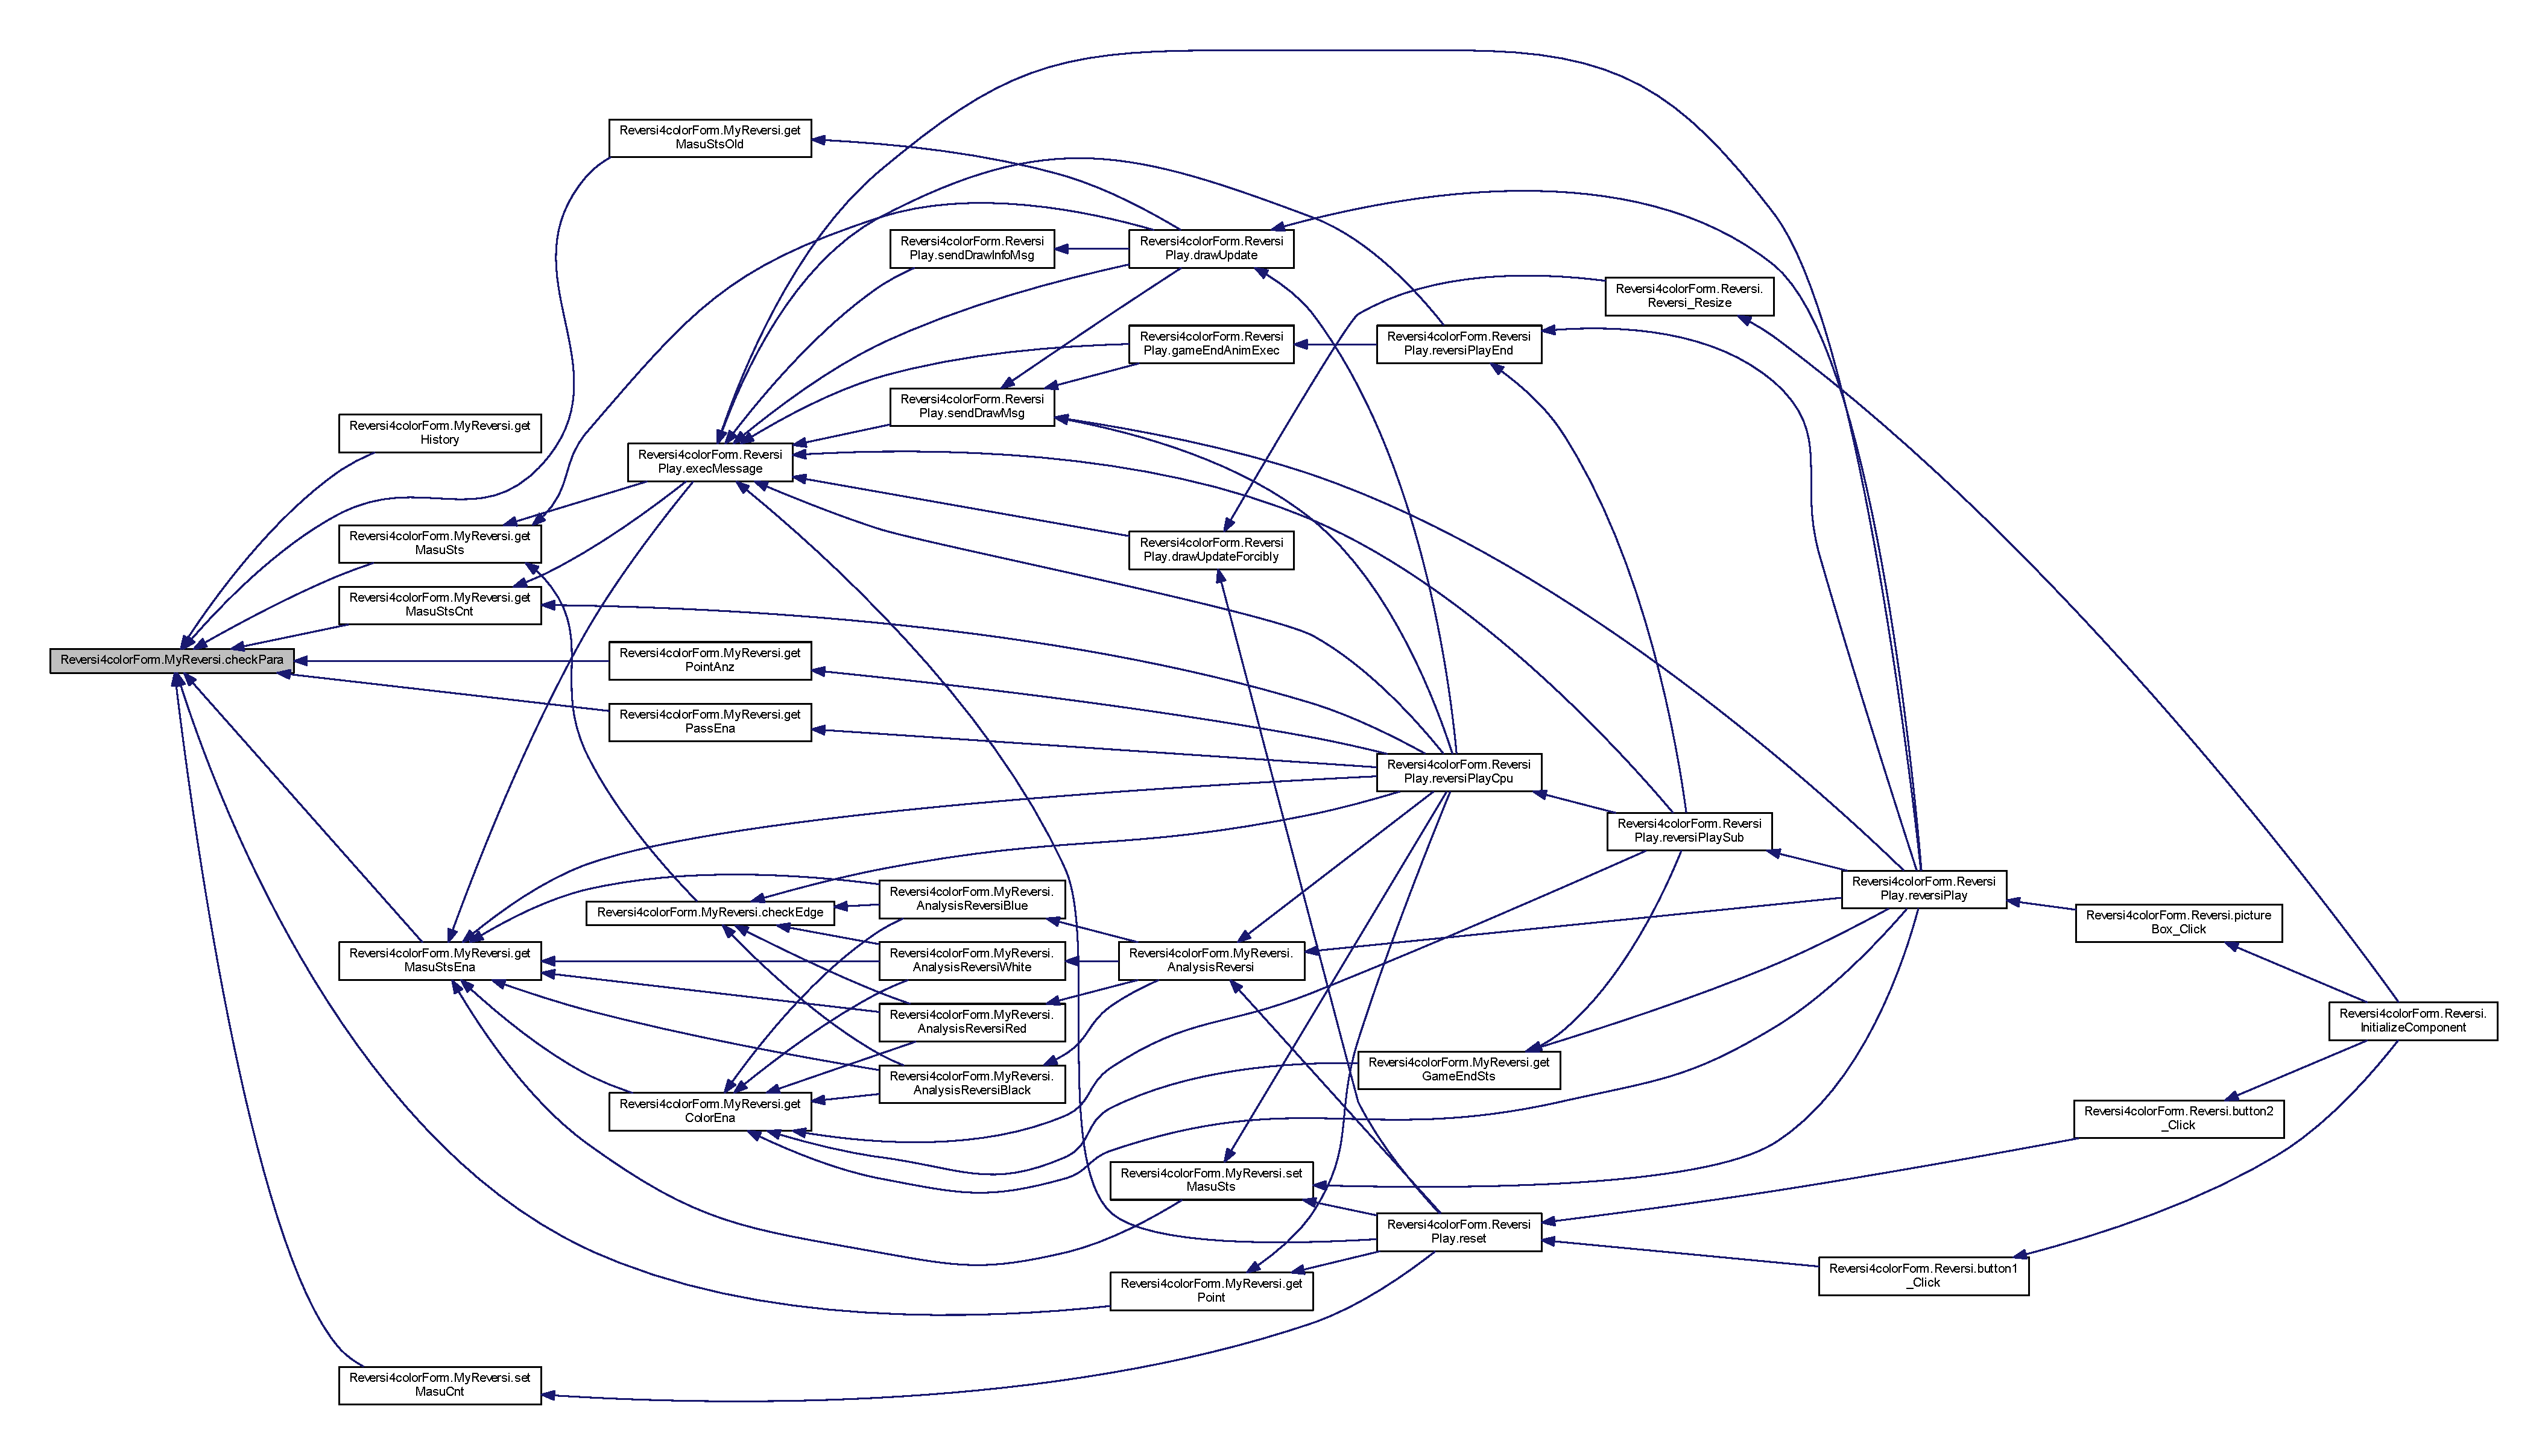
\includegraphics[width=350pt]{class_reversi4color_form_1_1_my_reversi_a02c145ac89302f2360cdb0c0391a38ce_icgraph}
\end{center}
\end{figure}
\mbox{\Hypertarget{class_reversi4color_form_1_1_my_reversi_a45ce9de1a7d3209c2ad6c256ad1c4fe8}\label{class_reversi4color_form_1_1_my_reversi_a45ce9de1a7d3209c2ad6c256ad1c4fe8}} 
\index{Reversi4color\+Form\+::\+My\+Reversi@{Reversi4color\+Form\+::\+My\+Reversi}!Clone@{Clone}}
\index{Clone@{Clone}!Reversi4color\+Form\+::\+My\+Reversi@{Reversi4color\+Form\+::\+My\+Reversi}}
\subsubsection{\texorpdfstring{Clone()}{Clone()}}
{\footnotesize\ttfamily \hyperlink{class_reversi4color_form_1_1_my_reversi}{My\+Reversi} Reversi4color\+Form.\+My\+Reversi.\+Clone (\begin{DoxyParamCaption}{ }\end{DoxyParamCaption})}



コピー 

\begin{DoxyReturn}{Returns}
オブジェクトコピー 
\end{DoxyReturn}
\begin{DoxyAuthor}{Author}
Yuta Yoshinaga 
\end{DoxyAuthor}
\begin{DoxyDate}{Date}
2017.\+10.\+20 
\end{DoxyDate}


Definition at line 342 of file My\+Reversi.\+cs.

\mbox{\Hypertarget{class_reversi4color_form_1_1_my_reversi_ae184f1817b7dfac87613179e3e7e9124}\label{class_reversi4color_form_1_1_my_reversi_ae184f1817b7dfac87613179e3e7e9124}} 
\index{Reversi4color\+Form\+::\+My\+Reversi@{Reversi4color\+Form\+::\+My\+Reversi}!get\+Bet\+Cnt@{get\+Bet\+Cnt}}
\index{get\+Bet\+Cnt@{get\+Bet\+Cnt}!Reversi4color\+Form\+::\+My\+Reversi@{Reversi4color\+Form\+::\+My\+Reversi}}
\subsubsection{\texorpdfstring{get\+Bet\+Cnt()}{getBetCnt()}}
{\footnotesize\ttfamily int Reversi4color\+Form.\+My\+Reversi.\+get\+Bet\+Cnt (\begin{DoxyParamCaption}\item[{int}]{color }\end{DoxyParamCaption})}



コマ数取得 


\begin{DoxyParams}[1]{Parameters}
\mbox{\tt in}  & {\em int} & color コマ色 \\
\hline
\end{DoxyParams}
\begin{DoxyReturn}{Returns}
コマ数取得 
\end{DoxyReturn}
\begin{DoxyAuthor}{Author}
Yuta Yoshinaga 
\end{DoxyAuthor}
\begin{DoxyDate}{Date}
2017.\+10.\+20 
\end{DoxyDate}


Definition at line 1921 of file My\+Reversi.\+cs.



Referenced by Reversi4color\+Form.\+Reversi\+Play.\+exec\+Message(), Reversi4color\+Form.\+Reversi\+Play.\+game\+End\+Anim\+Exec(), Reversi4color\+Form.\+Reversi\+Play.\+reversi\+Play(), Reversi4color\+Form.\+Reversi\+Play.\+reversi\+Play\+Cpu(), Reversi4color\+Form.\+Reversi\+Play.\+reversi\+Play\+End(), and Reversi4color\+Form.\+Reversi\+Play.\+reversi\+Play\+Sub().

Here is the caller graph for this function\+:\nopagebreak
\begin{figure}[H]
\begin{center}
\leavevmode
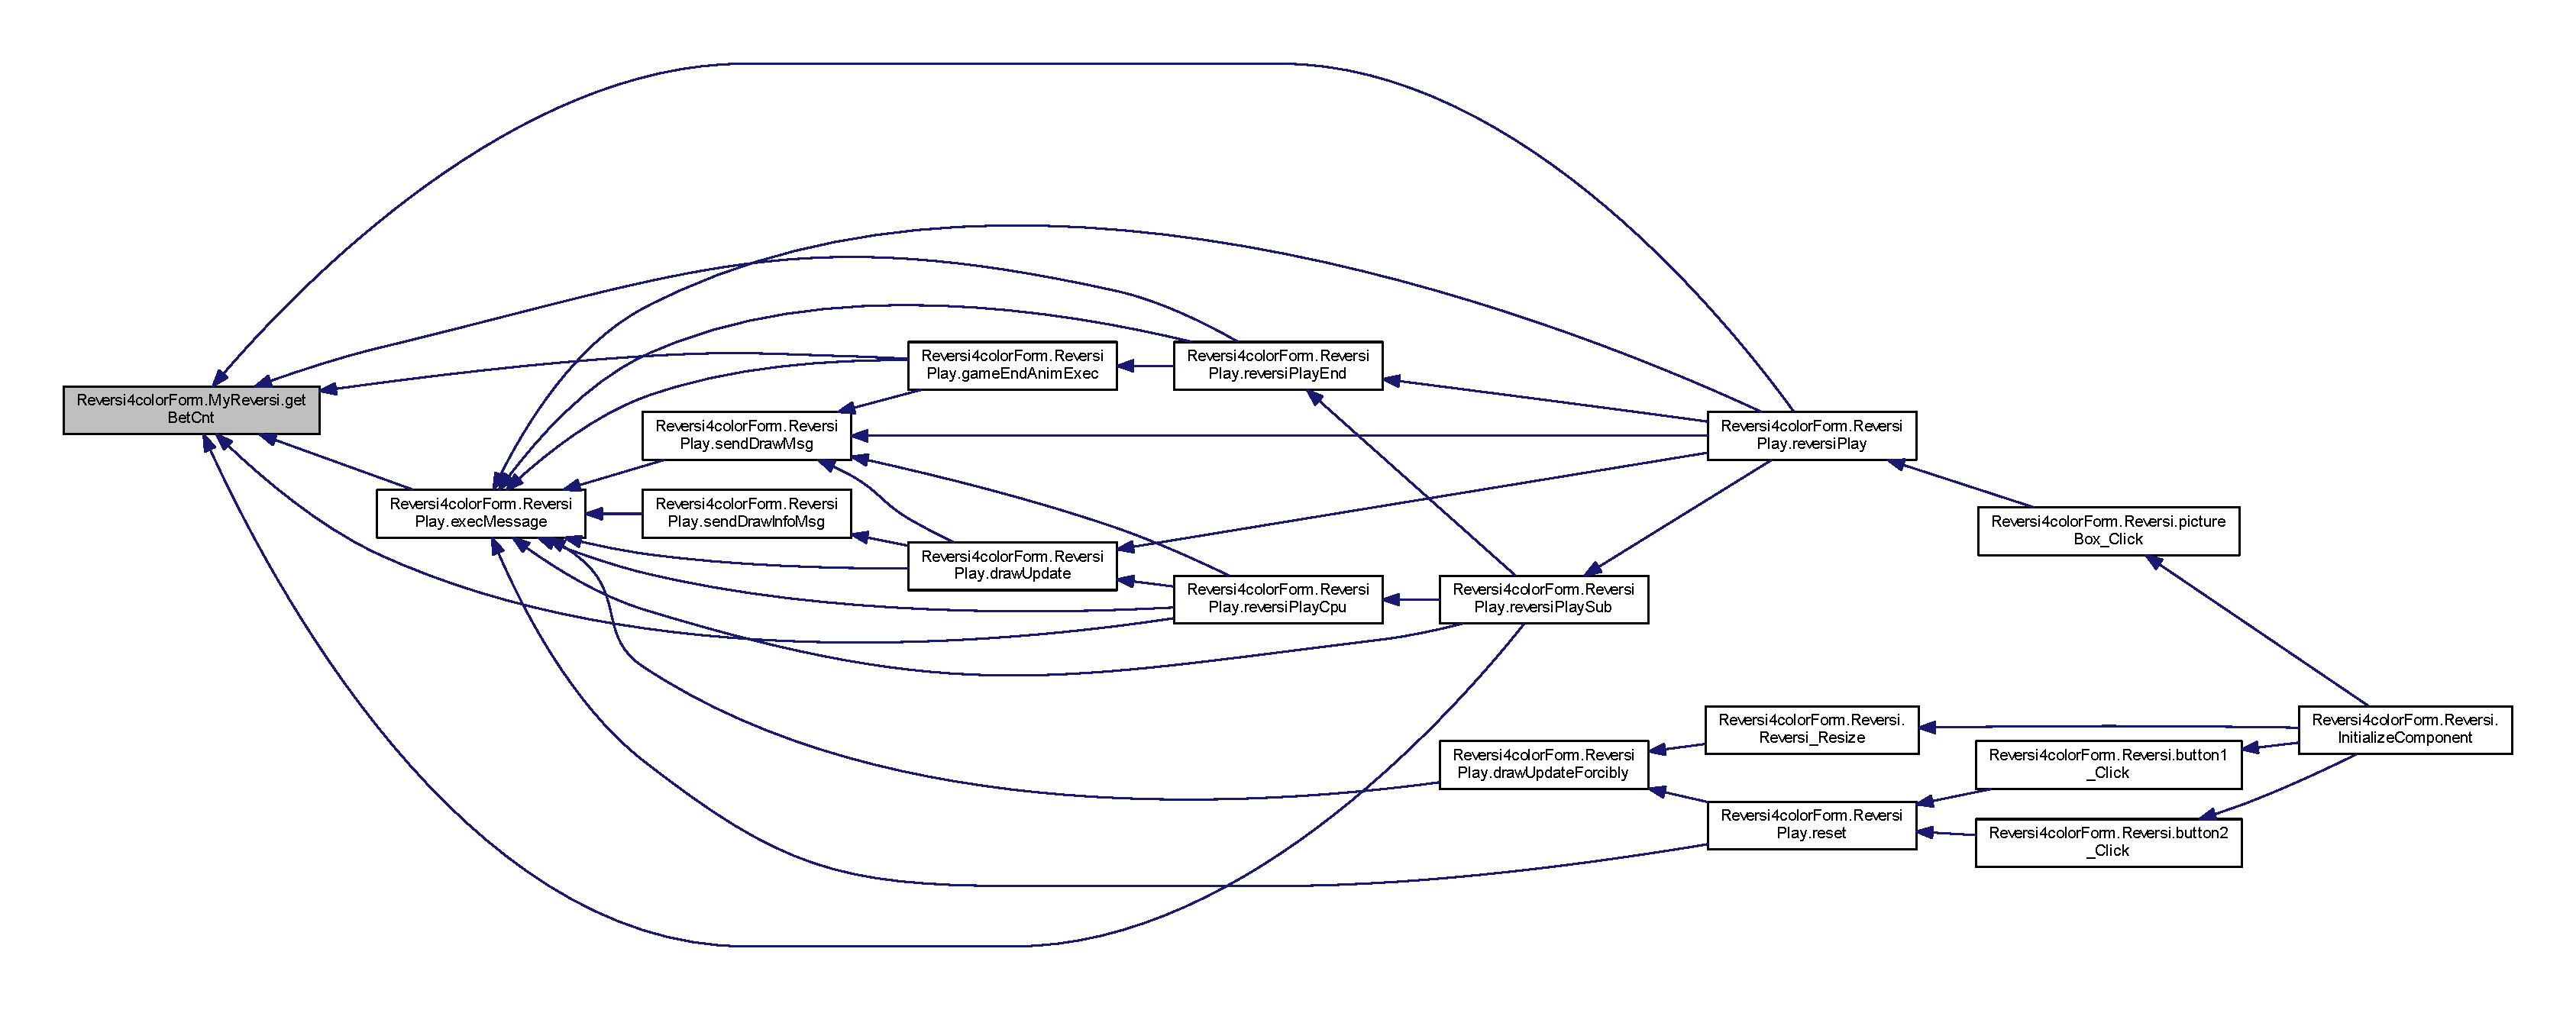
\includegraphics[width=350pt]{class_reversi4color_form_1_1_my_reversi_ae184f1817b7dfac87613179e3e7e9124_icgraph}
\end{center}
\end{figure}
\mbox{\Hypertarget{class_reversi4color_form_1_1_my_reversi_a5c18ae70cd8a10fee96f44e3a0e8621b}\label{class_reversi4color_form_1_1_my_reversi_a5c18ae70cd8a10fee96f44e3a0e8621b}} 
\index{Reversi4color\+Form\+::\+My\+Reversi@{Reversi4color\+Form\+::\+My\+Reversi}!get\+Color\+Ena@{get\+Color\+Ena}}
\index{get\+Color\+Ena@{get\+Color\+Ena}!Reversi4color\+Form\+::\+My\+Reversi@{Reversi4color\+Form\+::\+My\+Reversi}}
\subsubsection{\texorpdfstring{get\+Color\+Ena()}{getColorEna()}}
{\footnotesize\ttfamily int Reversi4color\+Form.\+My\+Reversi.\+get\+Color\+Ena (\begin{DoxyParamCaption}\item[{int}]{color }\end{DoxyParamCaption})}



指定色が現在置ける場所があるかチェック 


\begin{DoxyParams}[1]{Parameters}
\mbox{\tt in}  & {\em int} & color コマ色 \\
\hline
\end{DoxyParams}
\begin{DoxyReturn}{Returns}
0 \+: 成功 それ以外 \+: 失敗 
\end{DoxyReturn}
\begin{DoxyAuthor}{Author}
Yuta Yoshinaga 
\end{DoxyAuthor}
\begin{DoxyDate}{Date}
2017.\+10.\+20 
\end{DoxyDate}


Definition at line 1761 of file My\+Reversi.\+cs.



Referenced by Reversi4color\+Form.\+My\+Reversi.\+Analysis\+Reversi\+Black(), Reversi4color\+Form.\+My\+Reversi.\+Analysis\+Reversi\+Blue(), Reversi4color\+Form.\+My\+Reversi.\+Analysis\+Reversi\+Red(), Reversi4color\+Form.\+My\+Reversi.\+Analysis\+Reversi\+White(), Reversi4color\+Form.\+My\+Reversi.\+get\+Game\+End\+Sts(), Reversi4color\+Form.\+Reversi\+Play.\+reversi\+Play(), and Reversi4color\+Form.\+Reversi\+Play.\+reversi\+Play\+Sub().

Here is the call graph for this function\+:\nopagebreak
\begin{figure}[H]
\begin{center}
\leavevmode
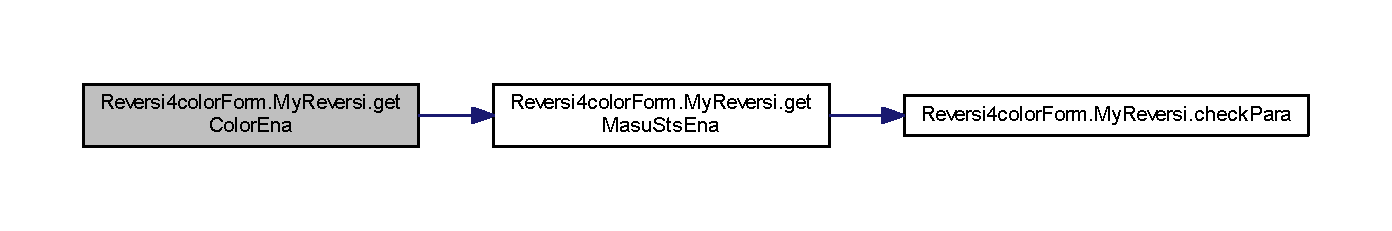
\includegraphics[width=350pt]{class_reversi4color_form_1_1_my_reversi_a5c18ae70cd8a10fee96f44e3a0e8621b_cgraph}
\end{center}
\end{figure}
Here is the caller graph for this function\+:\nopagebreak
\begin{figure}[H]
\begin{center}
\leavevmode
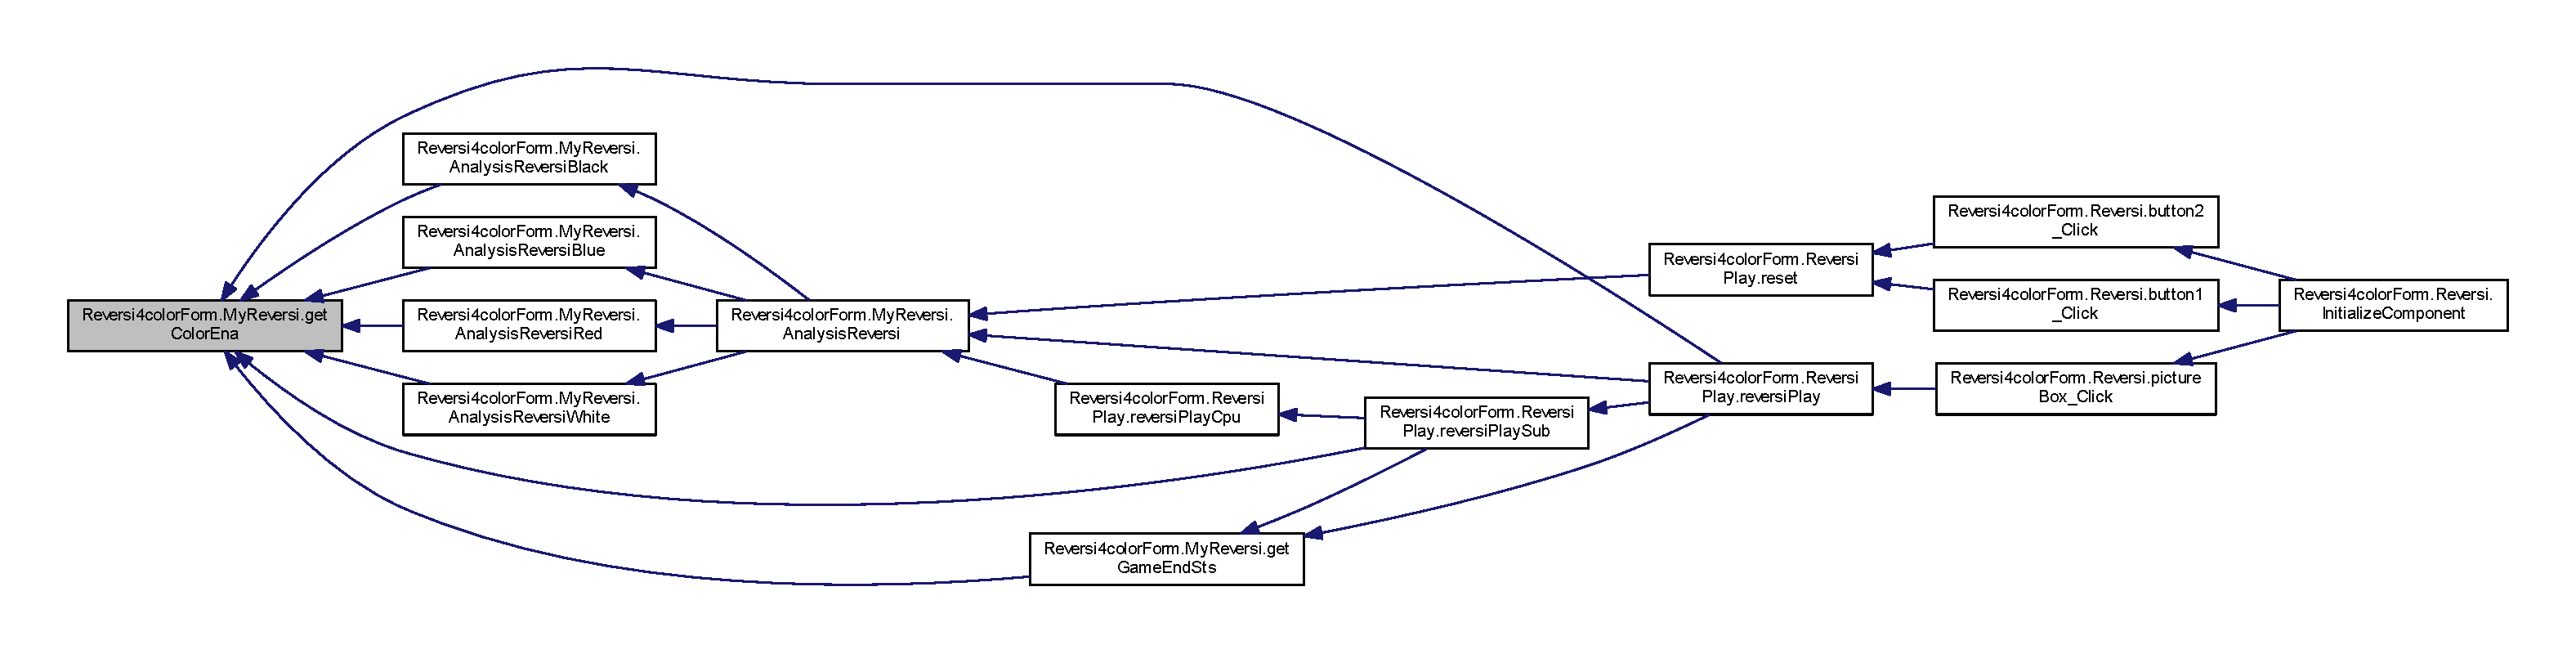
\includegraphics[width=350pt]{class_reversi4color_form_1_1_my_reversi_a5c18ae70cd8a10fee96f44e3a0e8621b_icgraph}
\end{center}
\end{figure}
\mbox{\Hypertarget{class_reversi4color_form_1_1_my_reversi_abf9583e4d29970acf85e662eb8a273dc}\label{class_reversi4color_form_1_1_my_reversi_abf9583e4d29970acf85e662eb8a273dc}} 
\index{Reversi4color\+Form\+::\+My\+Reversi@{Reversi4color\+Form\+::\+My\+Reversi}!get\+Edge\+Side\+One@{get\+Edge\+Side\+One}}
\index{get\+Edge\+Side\+One@{get\+Edge\+Side\+One}!Reversi4color\+Form\+::\+My\+Reversi@{Reversi4color\+Form\+::\+My\+Reversi}}
\subsubsection{\texorpdfstring{get\+Edge\+Side\+One()}{getEdgeSideOne()}}
{\footnotesize\ttfamily int Reversi4color\+Form.\+My\+Reversi.\+get\+Edge\+Side\+One (\begin{DoxyParamCaption}\item[{int}]{y,  }\item[{int}]{x }\end{DoxyParamCaption})}



指定座標が角の一つ手前か取得 


\begin{DoxyParams}[1]{Parameters}
\mbox{\tt in}  & {\em int} & y Y座標 \\
\hline
\mbox{\tt in}  & {\em int} & x X座標 \\
\hline
\end{DoxyParams}
\begin{DoxyReturn}{Returns}
0 \+: 成功 それ以外 \+: 失敗 
\end{DoxyReturn}
\begin{DoxyAuthor}{Author}
Yuta Yoshinaga 
\end{DoxyAuthor}
\begin{DoxyDate}{Date}
2017.\+10.\+20 
\end{DoxyDate}


Definition at line 2166 of file My\+Reversi.\+cs.



Referenced by Reversi4color\+Form.\+My\+Reversi.\+Analysis\+Reversi\+Black(), Reversi4color\+Form.\+My\+Reversi.\+Analysis\+Reversi\+Blue(), Reversi4color\+Form.\+My\+Reversi.\+Analysis\+Reversi\+Red(), Reversi4color\+Form.\+My\+Reversi.\+Analysis\+Reversi\+White(), and Reversi4color\+Form.\+Reversi\+Play.\+reversi\+Play\+Cpu().

Here is the caller graph for this function\+:\nopagebreak
\begin{figure}[H]
\begin{center}
\leavevmode
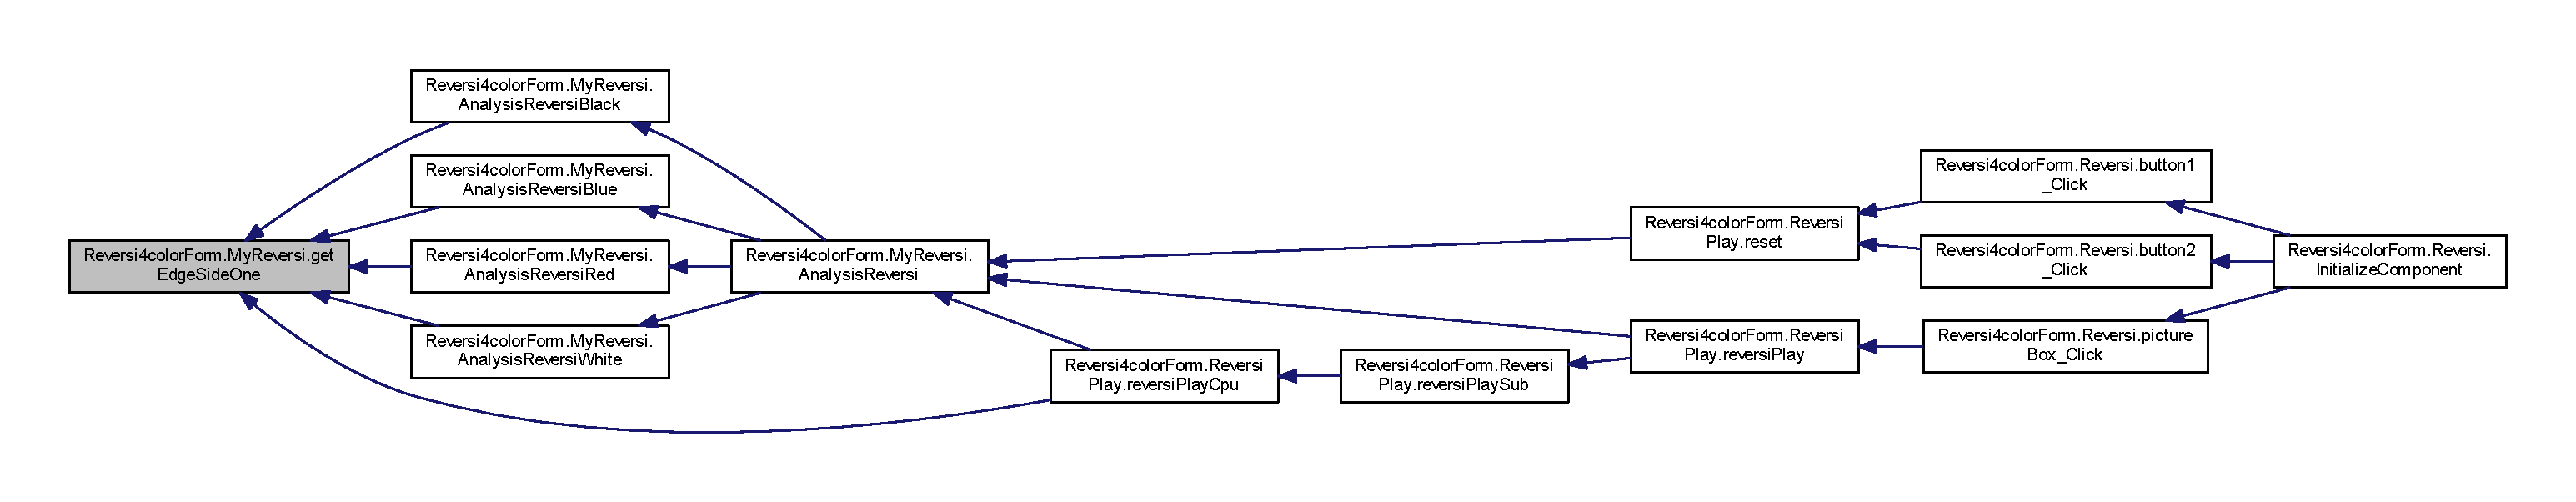
\includegraphics[width=350pt]{class_reversi4color_form_1_1_my_reversi_abf9583e4d29970acf85e662eb8a273dc_icgraph}
\end{center}
\end{figure}
\mbox{\Hypertarget{class_reversi4color_form_1_1_my_reversi_aca70a03939805aceed92fabb4a00636b}\label{class_reversi4color_form_1_1_my_reversi_aca70a03939805aceed92fabb4a00636b}} 
\index{Reversi4color\+Form\+::\+My\+Reversi@{Reversi4color\+Form\+::\+My\+Reversi}!get\+Edge\+Side\+Three@{get\+Edge\+Side\+Three}}
\index{get\+Edge\+Side\+Three@{get\+Edge\+Side\+Three}!Reversi4color\+Form\+::\+My\+Reversi@{Reversi4color\+Form\+::\+My\+Reversi}}
\subsubsection{\texorpdfstring{get\+Edge\+Side\+Three()}{getEdgeSideThree()}}
{\footnotesize\ttfamily int Reversi4color\+Form.\+My\+Reversi.\+get\+Edge\+Side\+Three (\begin{DoxyParamCaption}\item[{int}]{y,  }\item[{int}]{x }\end{DoxyParamCaption})}



指定座標が角の三つ以上手前か取得 


\begin{DoxyParams}[1]{Parameters}
\mbox{\tt in}  & {\em int} & y Y座標 \\
\hline
\mbox{\tt in}  & {\em int} & x X座標 \\
\hline
\end{DoxyParams}
\begin{DoxyReturn}{Returns}
0 \+: 成功 それ以外 \+: 失敗 
\end{DoxyReturn}
\begin{DoxyAuthor}{Author}
Yuta Yoshinaga 
\end{DoxyAuthor}
\begin{DoxyDate}{Date}
2017.\+10.\+20 
\end{DoxyDate}


Definition at line 2230 of file My\+Reversi.\+cs.



Referenced by Reversi4color\+Form.\+My\+Reversi.\+Analysis\+Reversi\+Black(), Reversi4color\+Form.\+My\+Reversi.\+Analysis\+Reversi\+Blue(), Reversi4color\+Form.\+My\+Reversi.\+Analysis\+Reversi\+Red(), Reversi4color\+Form.\+My\+Reversi.\+Analysis\+Reversi\+White(), and Reversi4color\+Form.\+Reversi\+Play.\+reversi\+Play\+Cpu().

Here is the caller graph for this function\+:\nopagebreak
\begin{figure}[H]
\begin{center}
\leavevmode
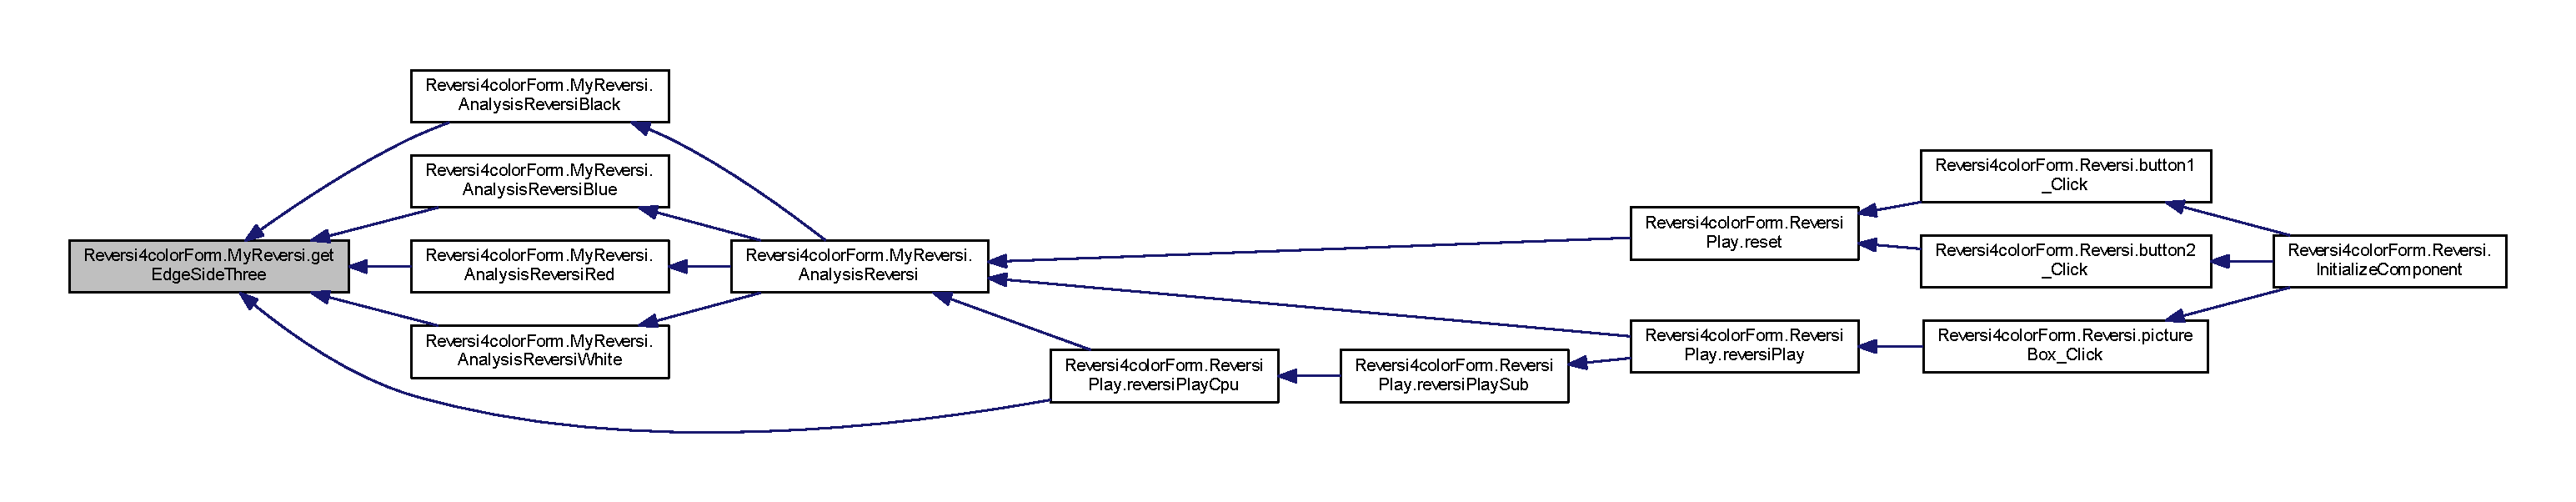
\includegraphics[width=350pt]{class_reversi4color_form_1_1_my_reversi_aca70a03939805aceed92fabb4a00636b_icgraph}
\end{center}
\end{figure}
\mbox{\Hypertarget{class_reversi4color_form_1_1_my_reversi_af5ccb42b478bf692989daef9c2495c53}\label{class_reversi4color_form_1_1_my_reversi_af5ccb42b478bf692989daef9c2495c53}} 
\index{Reversi4color\+Form\+::\+My\+Reversi@{Reversi4color\+Form\+::\+My\+Reversi}!get\+Edge\+Side\+Two@{get\+Edge\+Side\+Two}}
\index{get\+Edge\+Side\+Two@{get\+Edge\+Side\+Two}!Reversi4color\+Form\+::\+My\+Reversi@{Reversi4color\+Form\+::\+My\+Reversi}}
\subsubsection{\texorpdfstring{get\+Edge\+Side\+Two()}{getEdgeSideTwo()}}
{\footnotesize\ttfamily int Reversi4color\+Form.\+My\+Reversi.\+get\+Edge\+Side\+Two (\begin{DoxyParamCaption}\item[{int}]{y,  }\item[{int}]{x }\end{DoxyParamCaption})}



指定座標が角の二つ手前か取得 


\begin{DoxyParams}[1]{Parameters}
\mbox{\tt in}  & {\em int} & y Y座標 \\
\hline
\mbox{\tt in}  & {\em int} & x X座標 \\
\hline
\end{DoxyParams}
\begin{DoxyReturn}{Returns}
0 \+: 成功 それ以外 \+: 失敗 
\end{DoxyReturn}
\begin{DoxyAuthor}{Author}
Yuta Yoshinaga 
\end{DoxyAuthor}
\begin{DoxyDate}{Date}
2017.\+10.\+20 
\end{DoxyDate}


Definition at line 2198 of file My\+Reversi.\+cs.



Referenced by Reversi4color\+Form.\+My\+Reversi.\+Analysis\+Reversi\+Black(), Reversi4color\+Form.\+My\+Reversi.\+Analysis\+Reversi\+Blue(), Reversi4color\+Form.\+My\+Reversi.\+Analysis\+Reversi\+Red(), Reversi4color\+Form.\+My\+Reversi.\+Analysis\+Reversi\+White(), and Reversi4color\+Form.\+Reversi\+Play.\+reversi\+Play\+Cpu().

Here is the caller graph for this function\+:\nopagebreak
\begin{figure}[H]
\begin{center}
\leavevmode
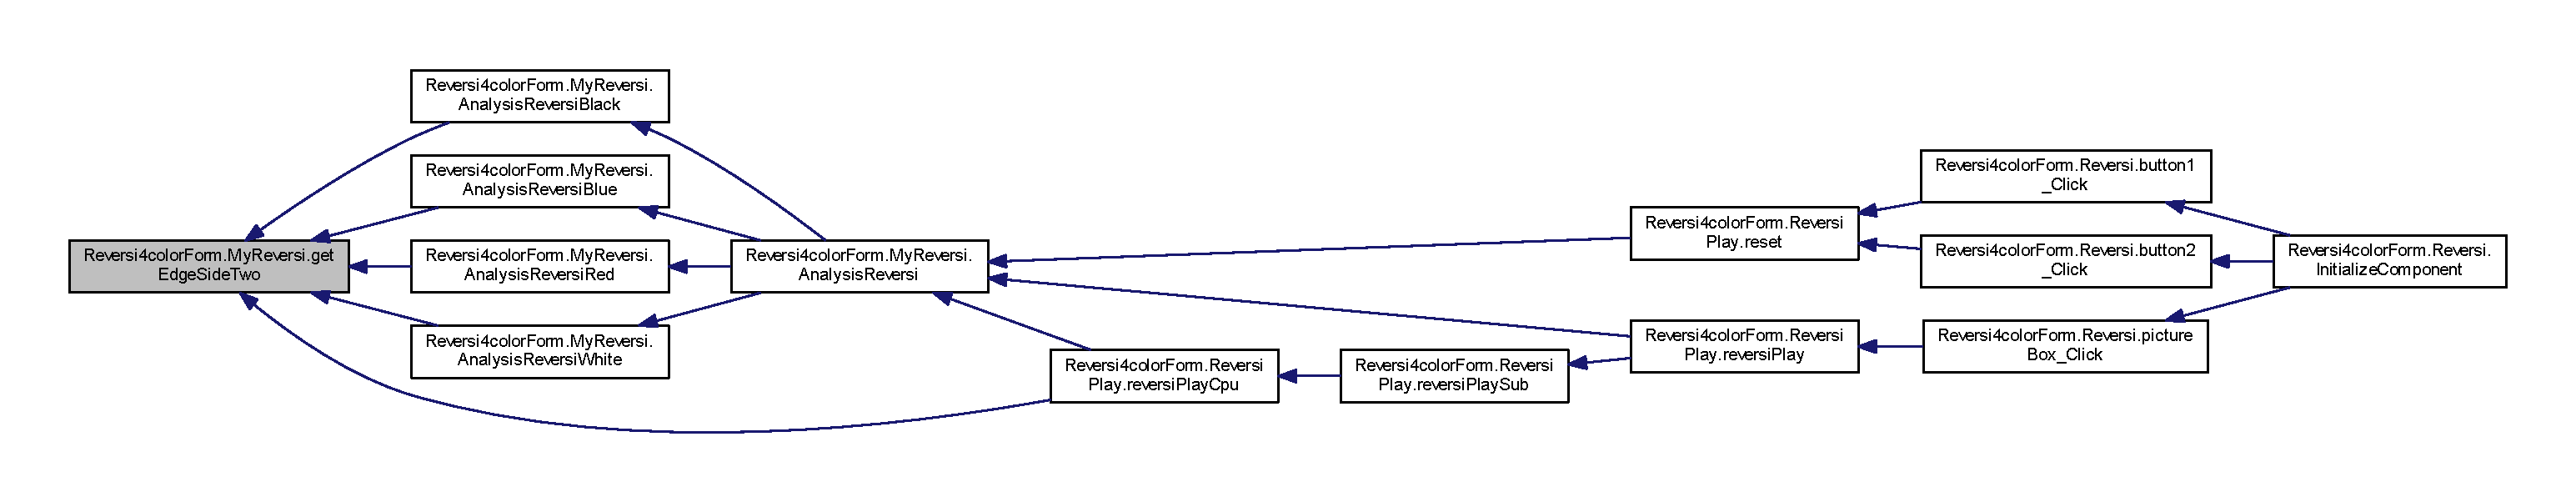
\includegraphics[width=350pt]{class_reversi4color_form_1_1_my_reversi_af5ccb42b478bf692989daef9c2495c53_icgraph}
\end{center}
\end{figure}
\mbox{\Hypertarget{class_reversi4color_form_1_1_my_reversi_a634f9e5deab1d15b929a33012acd03c2}\label{class_reversi4color_form_1_1_my_reversi_a634f9e5deab1d15b929a33012acd03c2}} 
\index{Reversi4color\+Form\+::\+My\+Reversi@{Reversi4color\+Form\+::\+My\+Reversi}!get\+Edge\+Side\+Zero@{get\+Edge\+Side\+Zero}}
\index{get\+Edge\+Side\+Zero@{get\+Edge\+Side\+Zero}!Reversi4color\+Form\+::\+My\+Reversi@{Reversi4color\+Form\+::\+My\+Reversi}}
\subsubsection{\texorpdfstring{get\+Edge\+Side\+Zero()}{getEdgeSideZero()}}
{\footnotesize\ttfamily int Reversi4color\+Form.\+My\+Reversi.\+get\+Edge\+Side\+Zero (\begin{DoxyParamCaption}\item[{int}]{y,  }\item[{int}]{x }\end{DoxyParamCaption})}



指定座標が角か取得 


\begin{DoxyParams}[1]{Parameters}
\mbox{\tt in}  & {\em int} & y Y座標 \\
\hline
\mbox{\tt in}  & {\em int} & x X座標 \\
\hline
\end{DoxyParams}
\begin{DoxyReturn}{Returns}
0 \+: 成功 それ以外 \+: 失敗 
\end{DoxyReturn}
\begin{DoxyAuthor}{Author}
Yuta Yoshinaga 
\end{DoxyAuthor}
\begin{DoxyDate}{Date}
2017.\+10.\+20 
\end{DoxyDate}


Definition at line 2142 of file My\+Reversi.\+cs.



Referenced by Reversi4color\+Form.\+My\+Reversi.\+Analysis\+Reversi\+Black(), Reversi4color\+Form.\+My\+Reversi.\+Analysis\+Reversi\+Blue(), Reversi4color\+Form.\+My\+Reversi.\+Analysis\+Reversi\+Red(), Reversi4color\+Form.\+My\+Reversi.\+Analysis\+Reversi\+White(), and Reversi4color\+Form.\+Reversi\+Play.\+reversi\+Play\+Cpu().

Here is the caller graph for this function\+:\nopagebreak
\begin{figure}[H]
\begin{center}
\leavevmode
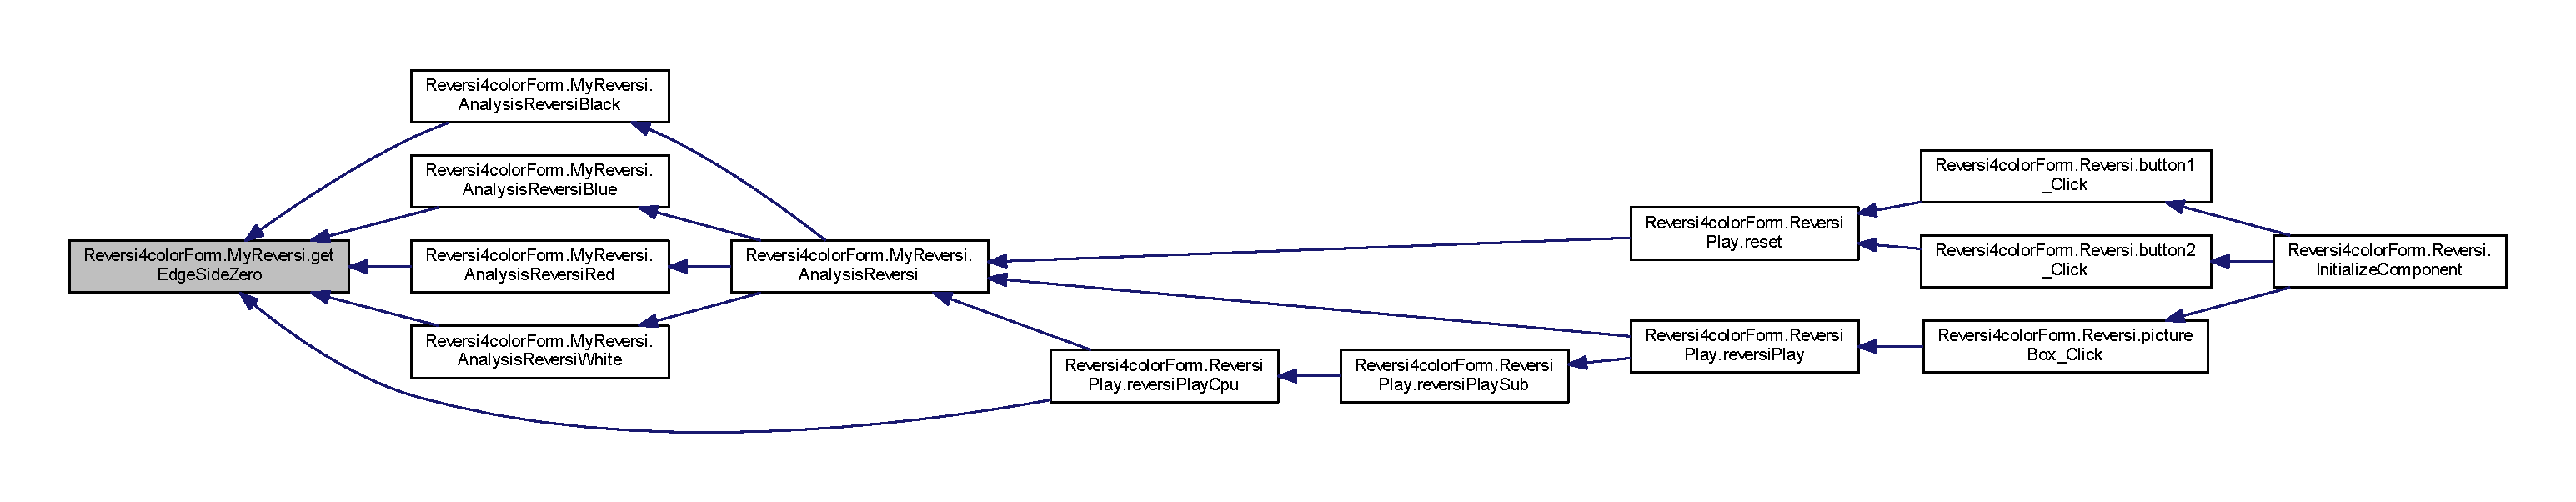
\includegraphics[width=350pt]{class_reversi4color_form_1_1_my_reversi_a634f9e5deab1d15b929a33012acd03c2_icgraph}
\end{center}
\end{figure}
\mbox{\Hypertarget{class_reversi4color_form_1_1_my_reversi_a5bdb21a8261d4af70bc2fabe7305ce22}\label{class_reversi4color_form_1_1_my_reversi_a5bdb21a8261d4af70bc2fabe7305ce22}} 
\index{Reversi4color\+Form\+::\+My\+Reversi@{Reversi4color\+Form\+::\+My\+Reversi}!get\+Game\+End\+Sts@{get\+Game\+End\+Sts}}
\index{get\+Game\+End\+Sts@{get\+Game\+End\+Sts}!Reversi4color\+Form\+::\+My\+Reversi@{Reversi4color\+Form\+::\+My\+Reversi}}
\subsubsection{\texorpdfstring{get\+Game\+End\+Sts()}{getGameEndSts()}}
{\footnotesize\ttfamily int Reversi4color\+Form.\+My\+Reversi.\+get\+Game\+End\+Sts (\begin{DoxyParamCaption}{ }\end{DoxyParamCaption})}



ゲーム終了かチェック 

\begin{DoxyReturn}{Returns}
0 \+: 続行 それ以外 \+: ゲーム終了 
\end{DoxyReturn}
\begin{DoxyAuthor}{Author}
Yuta Yoshinaga 
\end{DoxyAuthor}
\begin{DoxyDate}{Date}
2017.\+10.\+20 
\end{DoxyDate}


Definition at line 1783 of file My\+Reversi.\+cs.



Referenced by Reversi4color\+Form.\+Reversi\+Play.\+reversi\+Play(), and Reversi4color\+Form.\+Reversi\+Play.\+reversi\+Play\+Sub().

Here is the call graph for this function\+:\nopagebreak
\begin{figure}[H]
\begin{center}
\leavevmode
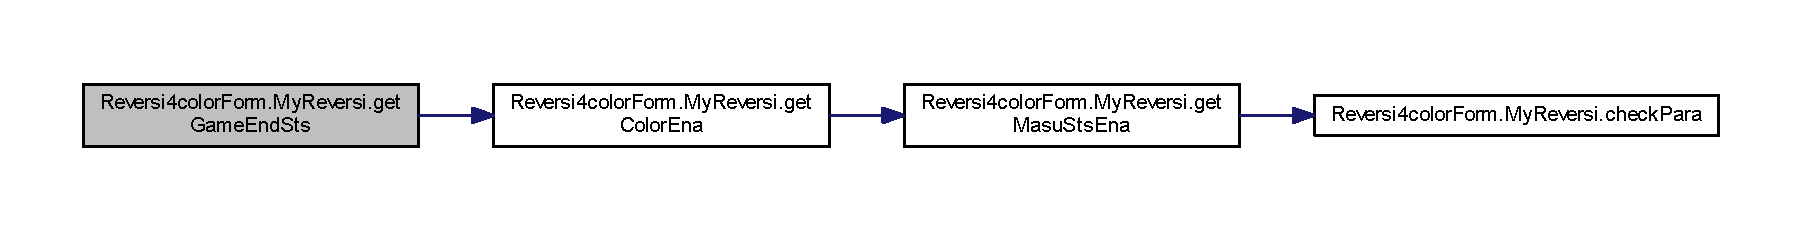
\includegraphics[width=350pt]{class_reversi4color_form_1_1_my_reversi_a5bdb21a8261d4af70bc2fabe7305ce22_cgraph}
\end{center}
\end{figure}
Here is the caller graph for this function\+:\nopagebreak
\begin{figure}[H]
\begin{center}
\leavevmode
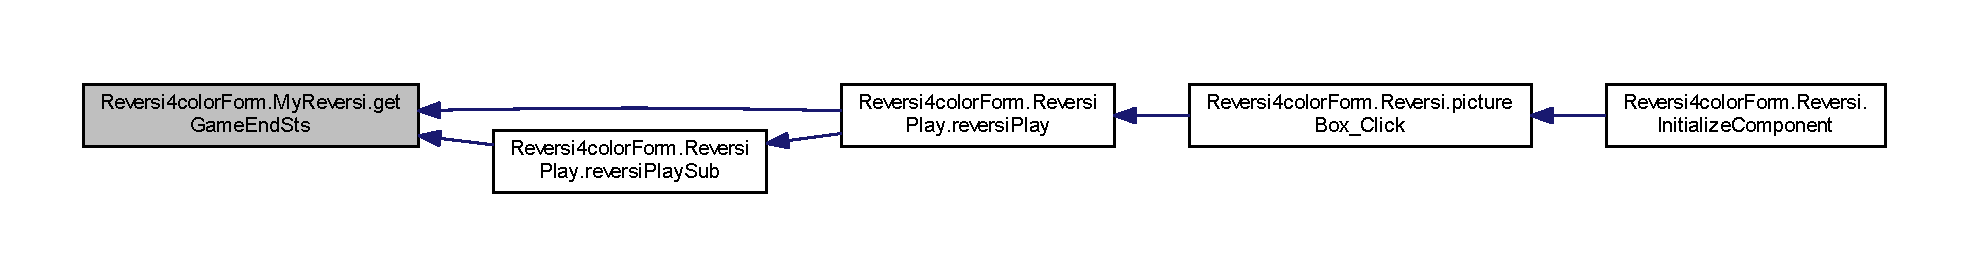
\includegraphics[width=350pt]{class_reversi4color_form_1_1_my_reversi_a5bdb21a8261d4af70bc2fabe7305ce22_icgraph}
\end{center}
\end{figure}
\mbox{\Hypertarget{class_reversi4color_form_1_1_my_reversi_a6765e90e98f20c7a19a941400446d006}\label{class_reversi4color_form_1_1_my_reversi_a6765e90e98f20c7a19a941400446d006}} 
\index{Reversi4color\+Form\+::\+My\+Reversi@{Reversi4color\+Form\+::\+My\+Reversi}!get\+History@{get\+History}}
\index{get\+History@{get\+History}!Reversi4color\+Form\+::\+My\+Reversi@{Reversi4color\+Form\+::\+My\+Reversi}}
\subsubsection{\texorpdfstring{get\+History()}{getHistory()}}
{\footnotesize\ttfamily \hyperlink{class_reversi4color_form_1_1_reversi_history}{Reversi\+History} Reversi4color\+Form.\+My\+Reversi.\+get\+History (\begin{DoxyParamCaption}\item[{int}]{num }\end{DoxyParamCaption})}



履歴取得 


\begin{DoxyParams}[1]{Parameters}
\mbox{\tt in}  & {\em int} & num ポイント \\
\hline
\end{DoxyParams}
\begin{DoxyReturn}{Returns}
履歴 null \+: 失敗 
\end{DoxyReturn}
\begin{DoxyAuthor}{Author}
Yuta Yoshinaga 
\end{DoxyAuthor}
\begin{DoxyDate}{Date}
2017.\+10.\+20 
\end{DoxyDate}


Definition at line 1966 of file My\+Reversi.\+cs.

Here is the call graph for this function\+:\nopagebreak
\begin{figure}[H]
\begin{center}
\leavevmode
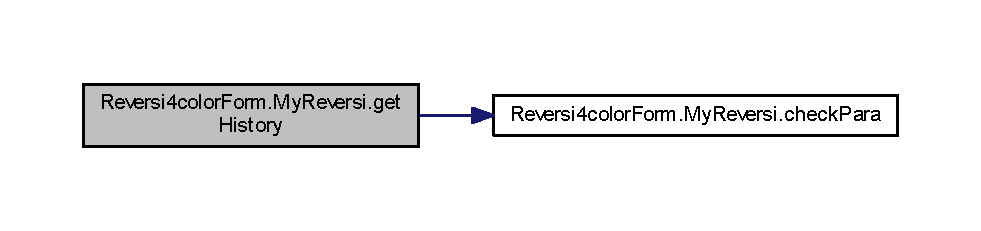
\includegraphics[width=350pt]{class_reversi4color_form_1_1_my_reversi_a6765e90e98f20c7a19a941400446d006_cgraph}
\end{center}
\end{figure}
\mbox{\Hypertarget{class_reversi4color_form_1_1_my_reversi_a9d4345e1a06f0d94f073f82037aa6113}\label{class_reversi4color_form_1_1_my_reversi_a9d4345e1a06f0d94f073f82037aa6113}} 
\index{Reversi4color\+Form\+::\+My\+Reversi@{Reversi4color\+Form\+::\+My\+Reversi}!get\+History\+Cnt@{get\+History\+Cnt}}
\index{get\+History\+Cnt@{get\+History\+Cnt}!Reversi4color\+Form\+::\+My\+Reversi@{Reversi4color\+Form\+::\+My\+Reversi}}
\subsubsection{\texorpdfstring{get\+History\+Cnt()}{getHistoryCnt()}}
{\footnotesize\ttfamily int Reversi4color\+Form.\+My\+Reversi.\+get\+History\+Cnt (\begin{DoxyParamCaption}{ }\end{DoxyParamCaption})}



履歴数取得 

\begin{DoxyReturn}{Returns}
履歴数 
\end{DoxyReturn}
\begin{DoxyAuthor}{Author}
Yuta Yoshinaga 
\end{DoxyAuthor}
\begin{DoxyDate}{Date}
2017.\+10.\+20 
\end{DoxyDate}


Definition at line 1983 of file My\+Reversi.\+cs.

\mbox{\Hypertarget{class_reversi4color_form_1_1_my_reversi_adc564d9d8aa75a871d33e09373485530}\label{class_reversi4color_form_1_1_my_reversi_adc564d9d8aa75a871d33e09373485530}} 
\index{Reversi4color\+Form\+::\+My\+Reversi@{Reversi4color\+Form\+::\+My\+Reversi}!get\+Masu\+Sts@{get\+Masu\+Sts}}
\index{get\+Masu\+Sts@{get\+Masu\+Sts}!Reversi4color\+Form\+::\+My\+Reversi@{Reversi4color\+Form\+::\+My\+Reversi}}
\subsubsection{\texorpdfstring{get\+Masu\+Sts()}{getMasuSts()}}
{\footnotesize\ttfamily int Reversi4color\+Form.\+My\+Reversi.\+get\+Masu\+Sts (\begin{DoxyParamCaption}\item[{int}]{y,  }\item[{int}]{x }\end{DoxyParamCaption})}



マスステータスを取得 


\begin{DoxyParams}[1]{Parameters}
\mbox{\tt in}  & {\em int} & y 取得するマスの\+Y座標 \\
\hline
\mbox{\tt in}  & {\em int} & x 取得するマスの\+X座標 \\
\hline
\end{DoxyParams}
\begin{DoxyReturn}{Returns}
-\/1 \+: 失敗 それ以外 \+: マスステータス 
\end{DoxyReturn}
\begin{DoxyAuthor}{Author}
Yuta Yoshinaga 
\end{DoxyAuthor}
\begin{DoxyDate}{Date}
2017.\+10.\+20 
\end{DoxyDate}


Definition at line 1682 of file My\+Reversi.\+cs.



Referenced by Reversi4color\+Form.\+My\+Reversi.\+check\+Edge(), Reversi4color\+Form.\+Reversi\+Play.\+draw\+Update(), and Reversi4color\+Form.\+Reversi\+Play.\+exec\+Message().

Here is the call graph for this function\+:\nopagebreak
\begin{figure}[H]
\begin{center}
\leavevmode
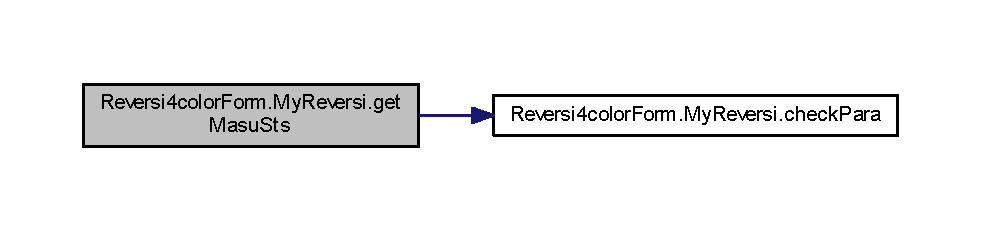
\includegraphics[width=350pt]{class_reversi4color_form_1_1_my_reversi_adc564d9d8aa75a871d33e09373485530_cgraph}
\end{center}
\end{figure}
Here is the caller graph for this function\+:\nopagebreak
\begin{figure}[H]
\begin{center}
\leavevmode
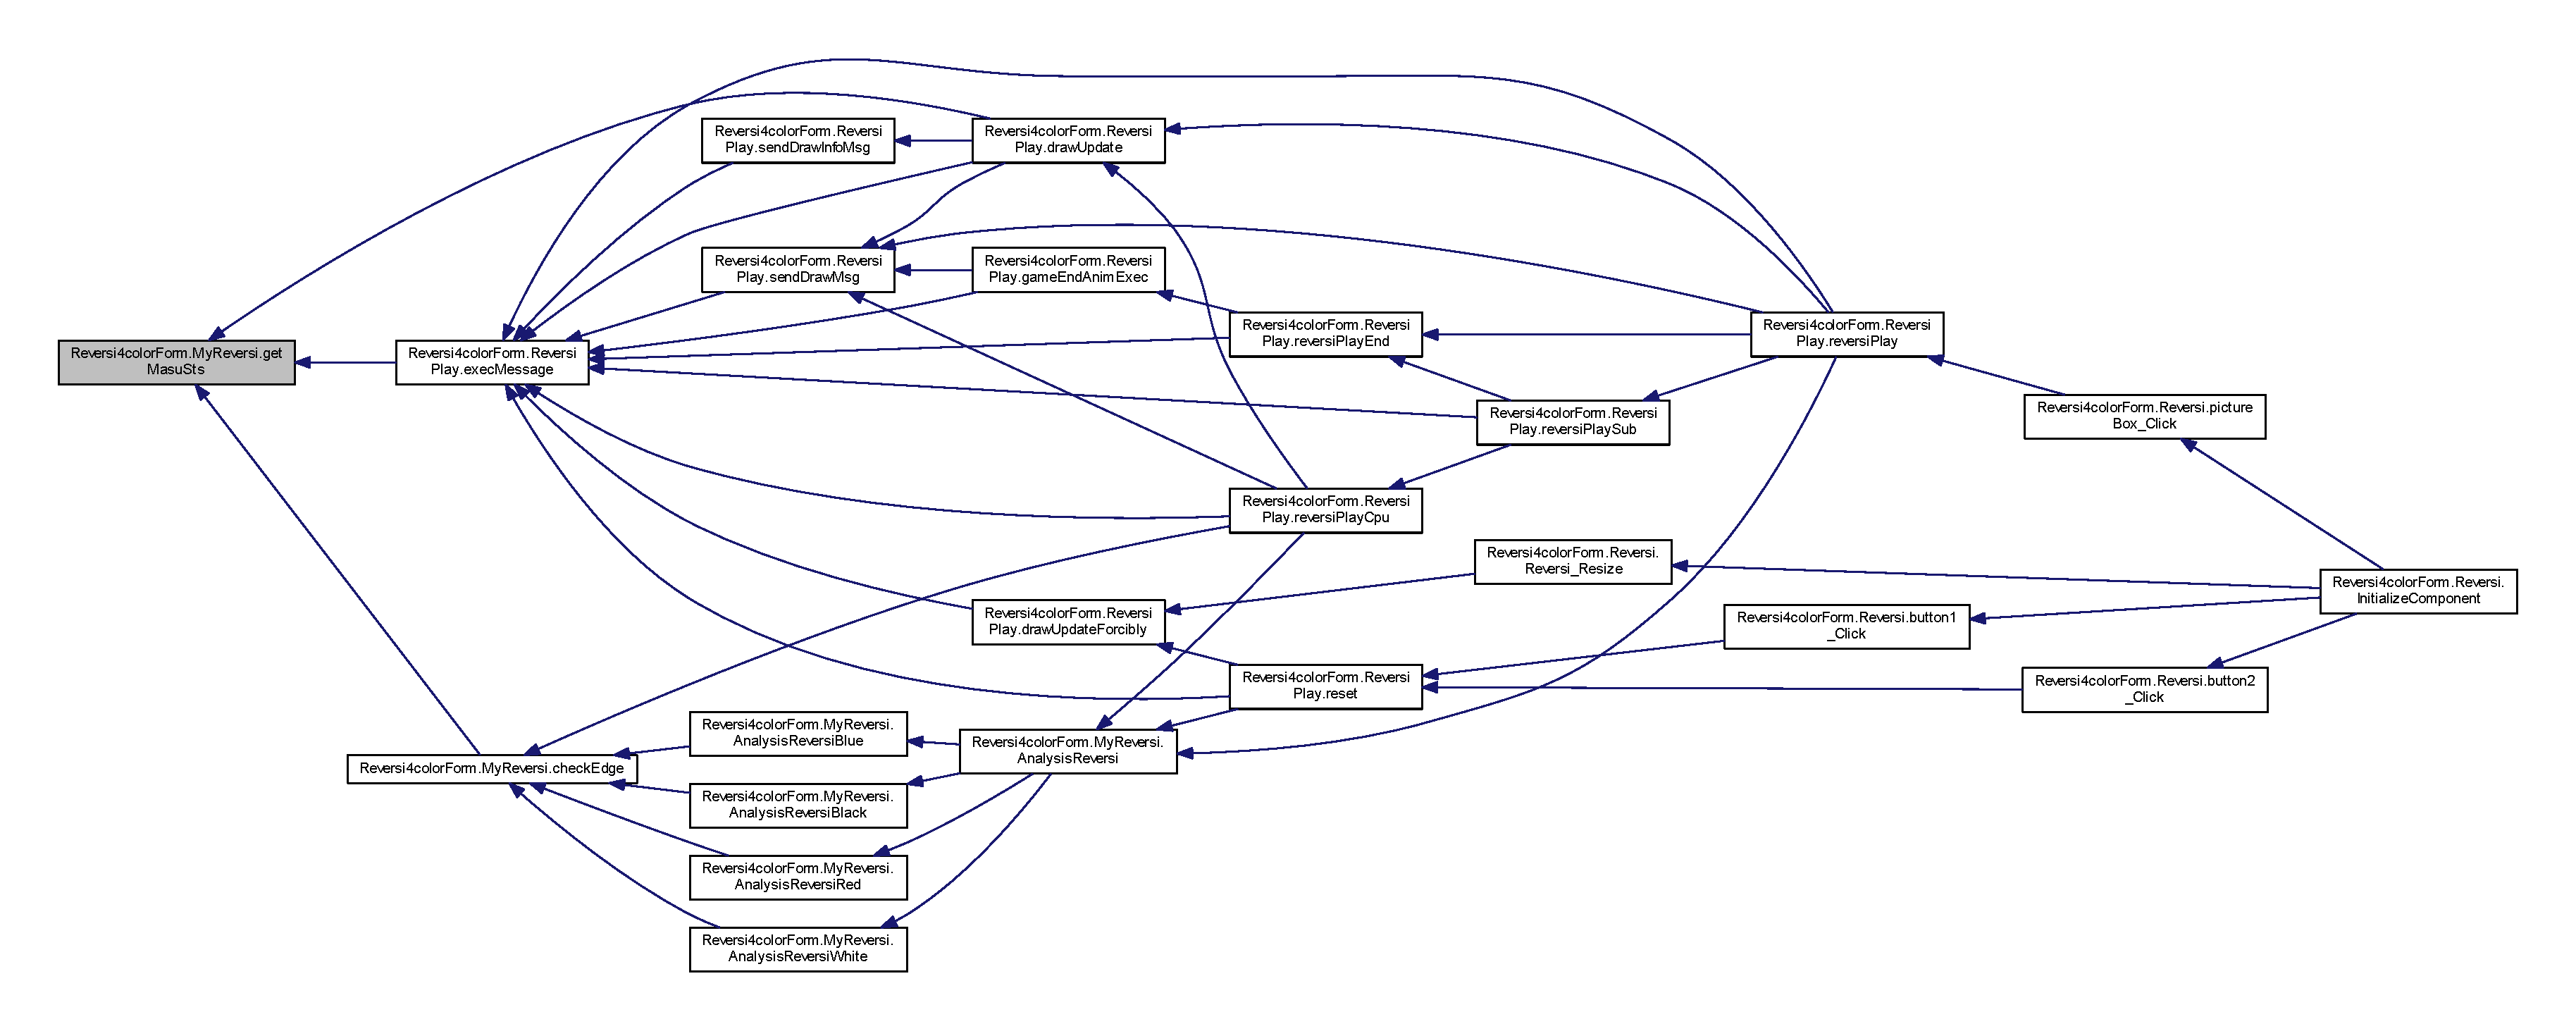
\includegraphics[width=350pt]{class_reversi4color_form_1_1_my_reversi_adc564d9d8aa75a871d33e09373485530_icgraph}
\end{center}
\end{figure}
\mbox{\Hypertarget{class_reversi4color_form_1_1_my_reversi_a5380e8f78bafedf7b0cdc86d943c8c22}\label{class_reversi4color_form_1_1_my_reversi_a5380e8f78bafedf7b0cdc86d943c8c22}} 
\index{Reversi4color\+Form\+::\+My\+Reversi@{Reversi4color\+Form\+::\+My\+Reversi}!get\+Masu\+Sts\+Cnt@{get\+Masu\+Sts\+Cnt}}
\index{get\+Masu\+Sts\+Cnt@{get\+Masu\+Sts\+Cnt}!Reversi4color\+Form\+::\+My\+Reversi@{Reversi4color\+Form\+::\+My\+Reversi}}
\subsubsection{\texorpdfstring{get\+Masu\+Sts\+Cnt()}{getMasuStsCnt()}}
{\footnotesize\ttfamily int Reversi4color\+Form.\+My\+Reversi.\+get\+Masu\+Sts\+Cnt (\begin{DoxyParamCaption}\item[{int}]{color,  }\item[{int}]{y,  }\item[{int}]{x }\end{DoxyParamCaption})}



指定座標の獲得コマ数取得 


\begin{DoxyParams}[1]{Parameters}
\mbox{\tt in}  & {\em int} & color コマ色 \\
\hline
\mbox{\tt in}  & {\em int} & y マスの\+Y座標 \\
\hline
\mbox{\tt in}  & {\em int} & x マスの\+X座標 \\
\hline
\end{DoxyParams}
\begin{DoxyReturn}{Returns}
-\/1 \+: 失敗 それ以外 \+: 獲得コマ数 
\end{DoxyReturn}
\begin{DoxyAuthor}{Author}
Yuta Yoshinaga 
\end{DoxyAuthor}
\begin{DoxyDate}{Date}
2017.\+10.\+20 
\end{DoxyDate}


Definition at line 1740 of file My\+Reversi.\+cs.



Referenced by Reversi4color\+Form.\+Reversi\+Play.\+exec\+Message(), and Reversi4color\+Form.\+Reversi\+Play.\+reversi\+Play\+Cpu().

Here is the call graph for this function\+:\nopagebreak
\begin{figure}[H]
\begin{center}
\leavevmode
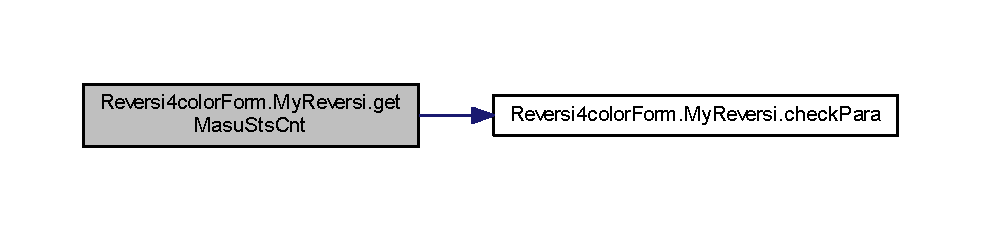
\includegraphics[width=350pt]{class_reversi4color_form_1_1_my_reversi_a5380e8f78bafedf7b0cdc86d943c8c22_cgraph}
\end{center}
\end{figure}
Here is the caller graph for this function\+:\nopagebreak
\begin{figure}[H]
\begin{center}
\leavevmode
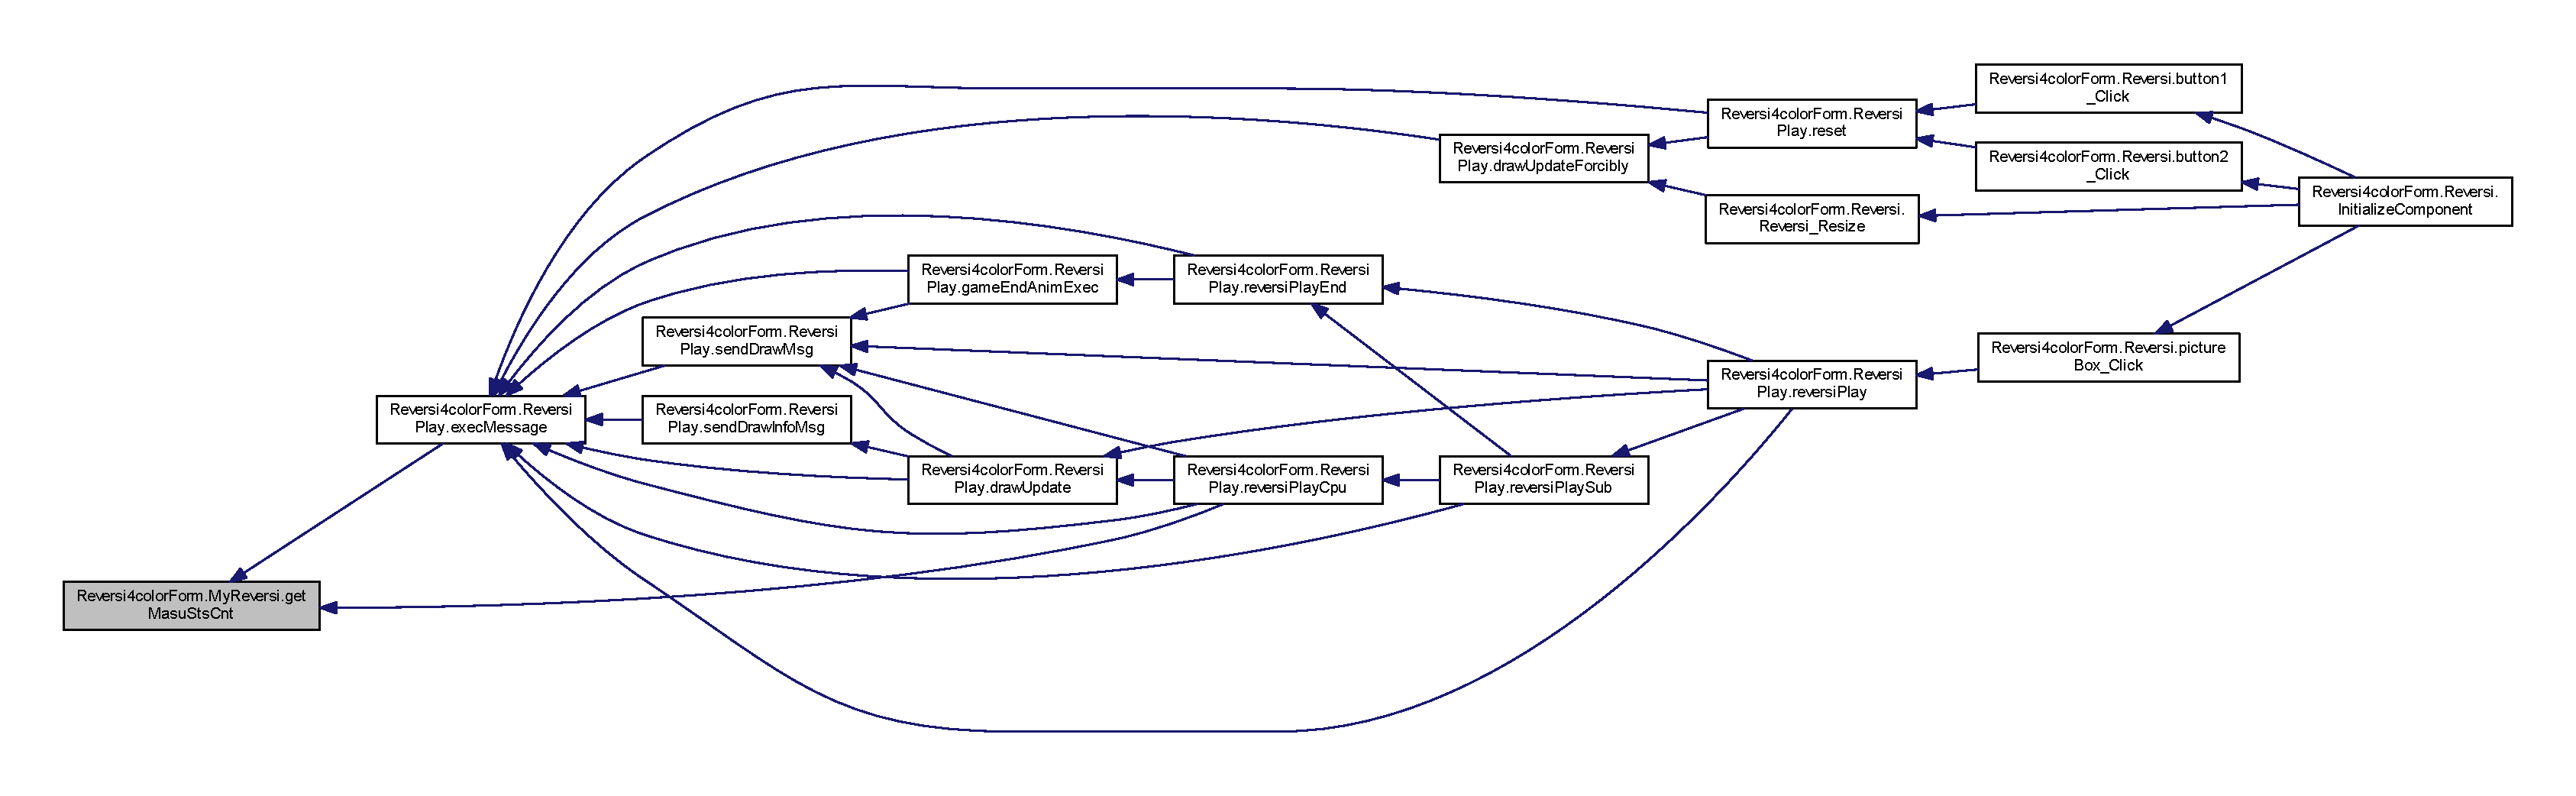
\includegraphics[width=350pt]{class_reversi4color_form_1_1_my_reversi_a5380e8f78bafedf7b0cdc86d943c8c22_icgraph}
\end{center}
\end{figure}
\mbox{\Hypertarget{class_reversi4color_form_1_1_my_reversi_ac17f7f56dd24fa06ac8d394290feafef}\label{class_reversi4color_form_1_1_my_reversi_ac17f7f56dd24fa06ac8d394290feafef}} 
\index{Reversi4color\+Form\+::\+My\+Reversi@{Reversi4color\+Form\+::\+My\+Reversi}!get\+Masu\+Sts\+Ena@{get\+Masu\+Sts\+Ena}}
\index{get\+Masu\+Sts\+Ena@{get\+Masu\+Sts\+Ena}!Reversi4color\+Form\+::\+My\+Reversi@{Reversi4color\+Form\+::\+My\+Reversi}}
\subsubsection{\texorpdfstring{get\+Masu\+Sts\+Ena()}{getMasuStsEna()}}
{\footnotesize\ttfamily int Reversi4color\+Form.\+My\+Reversi.\+get\+Masu\+Sts\+Ena (\begin{DoxyParamCaption}\item[{int}]{color,  }\item[{int}]{y,  }\item[{int}]{x }\end{DoxyParamCaption})}



指定座標に指定色を置けるかチェック 


\begin{DoxyParams}[1]{Parameters}
\mbox{\tt in}  & {\em int} & color コマ色 \\
\hline
\mbox{\tt in}  & {\em int} & y マスの\+Y座標 \\
\hline
\mbox{\tt in}  & {\em int} & x マスの\+X座標 \\
\hline
\end{DoxyParams}
\begin{DoxyReturn}{Returns}
1 \+: 成功 それ以外 \+: 失敗 
\end{DoxyReturn}
\begin{DoxyAuthor}{Author}
Yuta Yoshinaga 
\end{DoxyAuthor}
\begin{DoxyDate}{Date}
2017.\+10.\+20 
\end{DoxyDate}


Definition at line 1717 of file My\+Reversi.\+cs.



Referenced by Reversi4color\+Form.\+My\+Reversi.\+Analysis\+Reversi\+Black(), Reversi4color\+Form.\+My\+Reversi.\+Analysis\+Reversi\+Blue(), Reversi4color\+Form.\+My\+Reversi.\+Analysis\+Reversi\+Red(), Reversi4color\+Form.\+My\+Reversi.\+Analysis\+Reversi\+White(), Reversi4color\+Form.\+Reversi\+Play.\+exec\+Message(), Reversi4color\+Form.\+My\+Reversi.\+get\+Color\+Ena(), Reversi4color\+Form.\+Reversi\+Play.\+reversi\+Play\+Cpu(), and Reversi4color\+Form.\+My\+Reversi.\+set\+Masu\+Sts().

Here is the call graph for this function\+:\nopagebreak
\begin{figure}[H]
\begin{center}
\leavevmode
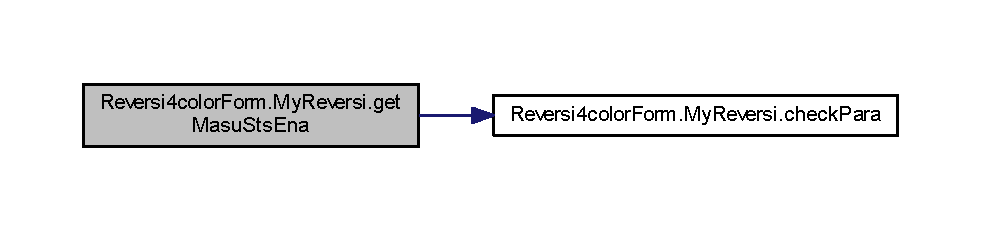
\includegraphics[width=350pt]{class_reversi4color_form_1_1_my_reversi_ac17f7f56dd24fa06ac8d394290feafef_cgraph}
\end{center}
\end{figure}
Here is the caller graph for this function\+:\nopagebreak
\begin{figure}[H]
\begin{center}
\leavevmode
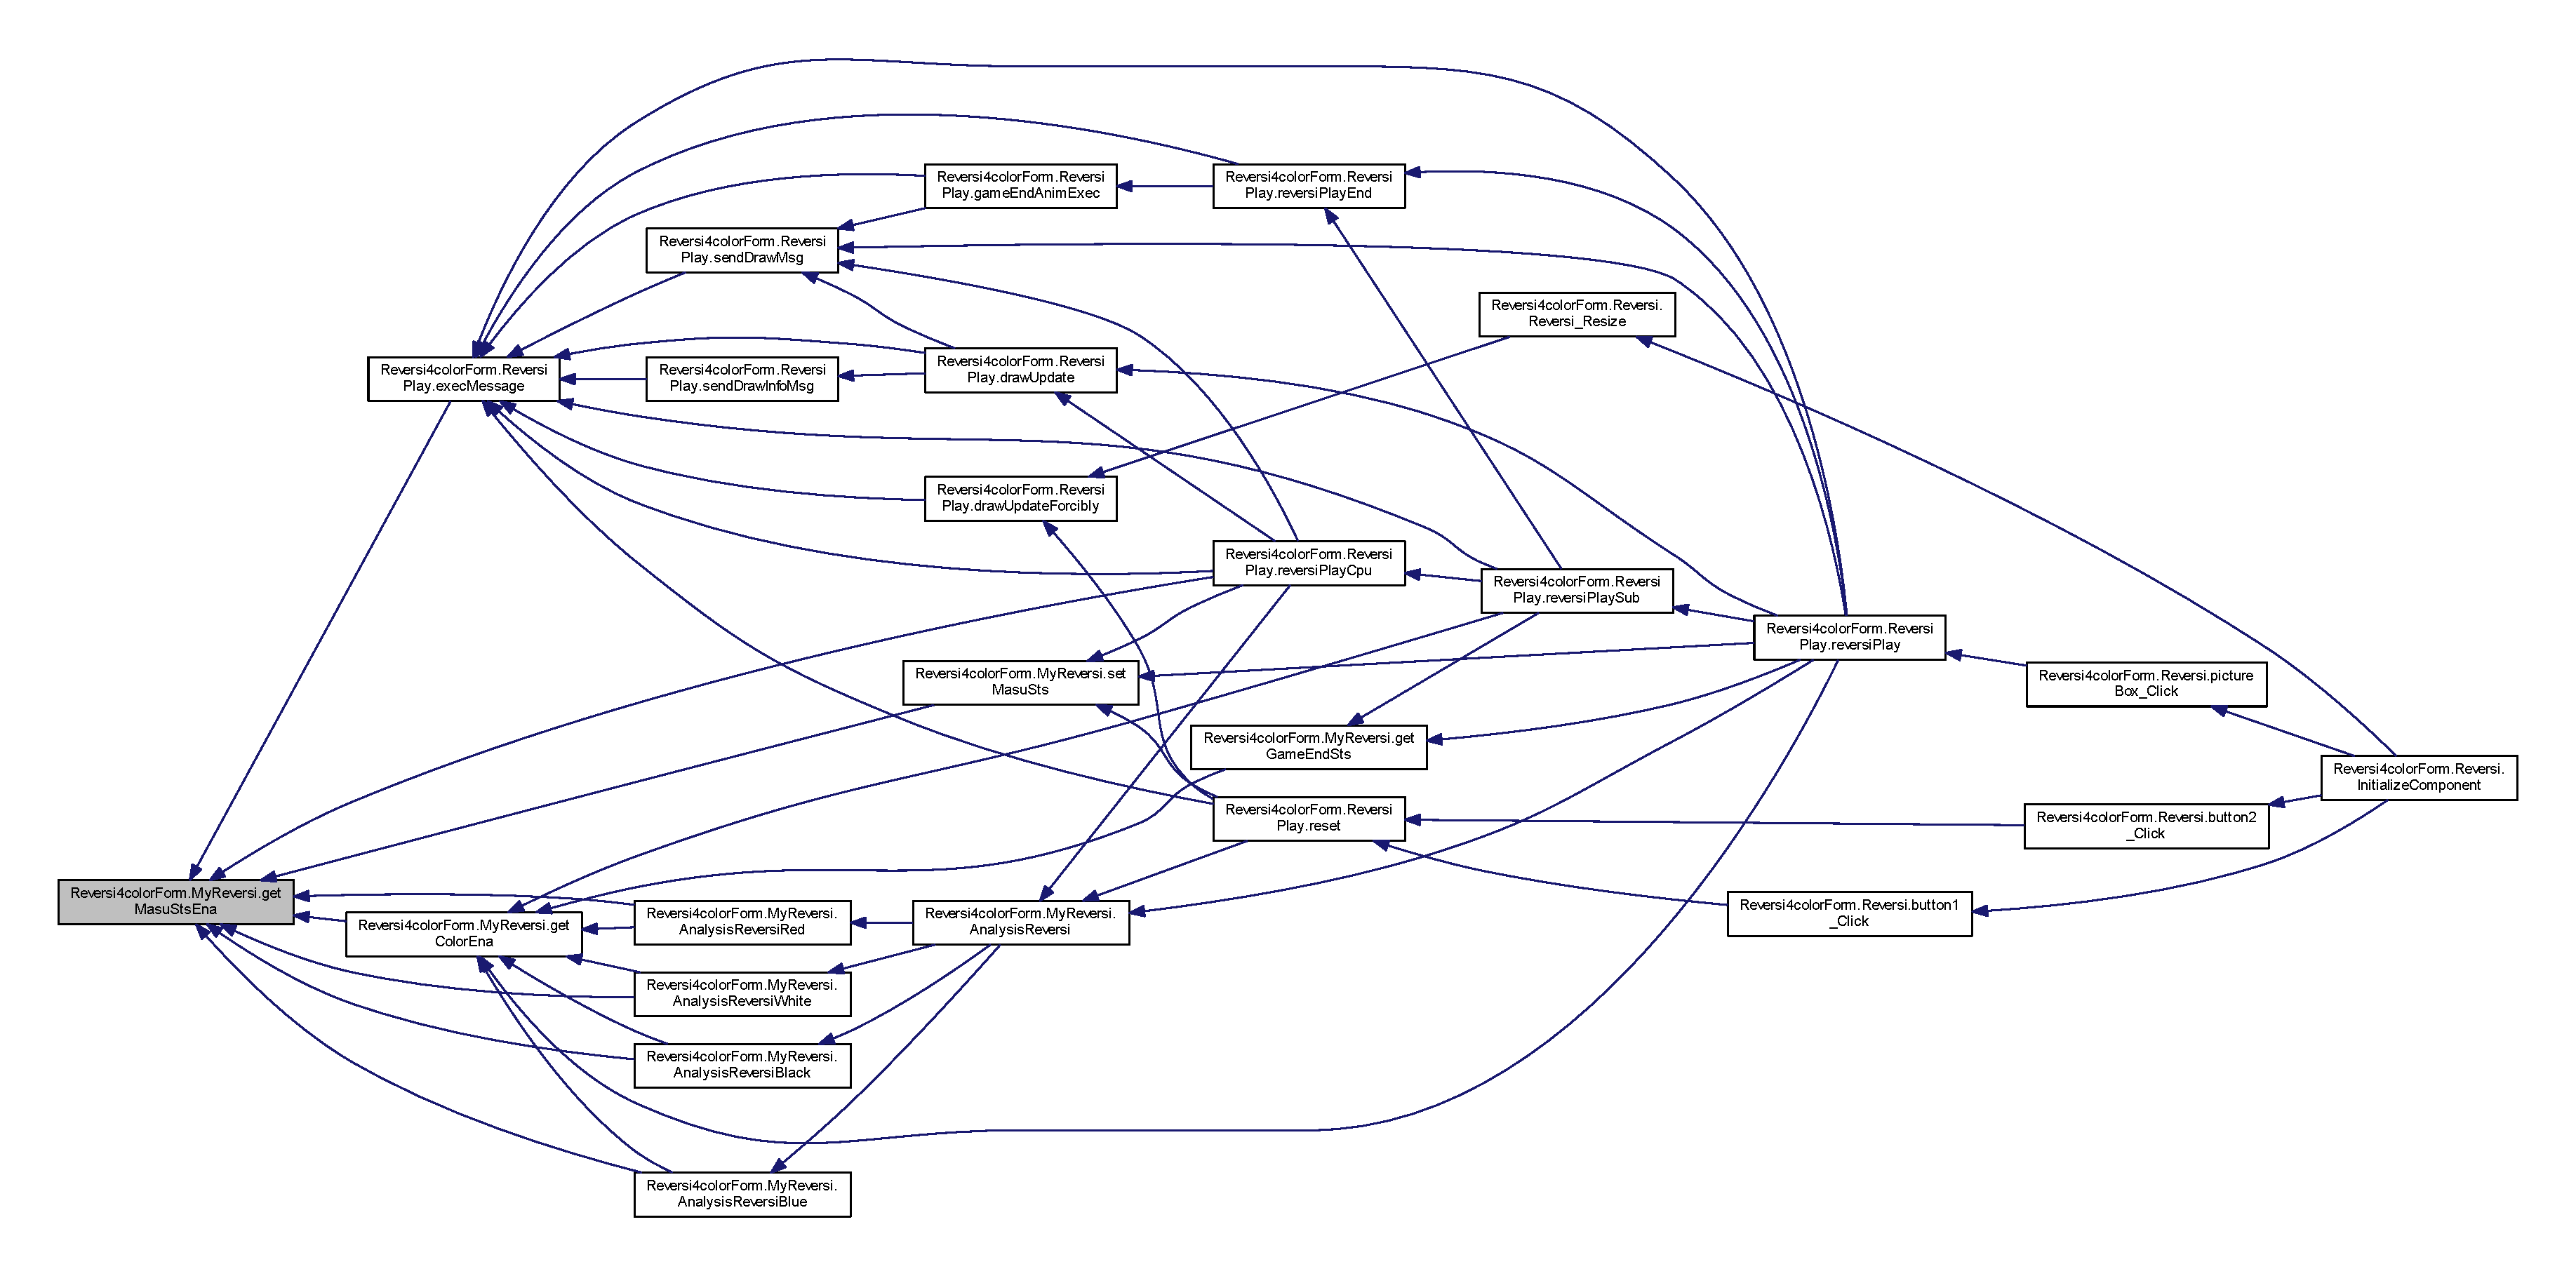
\includegraphics[width=350pt]{class_reversi4color_form_1_1_my_reversi_ac17f7f56dd24fa06ac8d394290feafef_icgraph}
\end{center}
\end{figure}
\mbox{\Hypertarget{class_reversi4color_form_1_1_my_reversi_aa56088eff96a48e68d4c7f688fe06b8d}\label{class_reversi4color_form_1_1_my_reversi_aa56088eff96a48e68d4c7f688fe06b8d}} 
\index{Reversi4color\+Form\+::\+My\+Reversi@{Reversi4color\+Form\+::\+My\+Reversi}!get\+Masu\+Sts\+Old@{get\+Masu\+Sts\+Old}}
\index{get\+Masu\+Sts\+Old@{get\+Masu\+Sts\+Old}!Reversi4color\+Form\+::\+My\+Reversi@{Reversi4color\+Form\+::\+My\+Reversi}}
\subsubsection{\texorpdfstring{get\+Masu\+Sts\+Old()}{getMasuStsOld()}}
{\footnotesize\ttfamily int Reversi4color\+Form.\+My\+Reversi.\+get\+Masu\+Sts\+Old (\begin{DoxyParamCaption}\item[{int}]{y,  }\item[{int}]{x }\end{DoxyParamCaption})}



以前のマスステータスを取得 


\begin{DoxyParams}[1]{Parameters}
\mbox{\tt in}  & {\em int} & y 取得するマスの\+Y座標 \\
\hline
\mbox{\tt in}  & {\em int} & x 取得するマスの\+X座標 \\
\hline
\end{DoxyParams}
\begin{DoxyReturn}{Returns}
-\/1 \+: 失敗 それ以外 \+: マスステータス 
\end{DoxyReturn}
\begin{DoxyAuthor}{Author}
Yuta Yoshinaga 
\end{DoxyAuthor}
\begin{DoxyDate}{Date}
2017.\+10.\+20 
\end{DoxyDate}


Definition at line 1699 of file My\+Reversi.\+cs.



Referenced by Reversi4color\+Form.\+Reversi\+Play.\+draw\+Update().

Here is the call graph for this function\+:\nopagebreak
\begin{figure}[H]
\begin{center}
\leavevmode
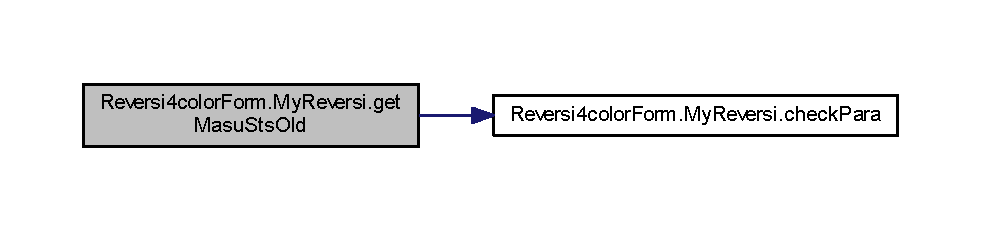
\includegraphics[width=350pt]{class_reversi4color_form_1_1_my_reversi_aa56088eff96a48e68d4c7f688fe06b8d_cgraph}
\end{center}
\end{figure}
Here is the caller graph for this function\+:\nopagebreak
\begin{figure}[H]
\begin{center}
\leavevmode
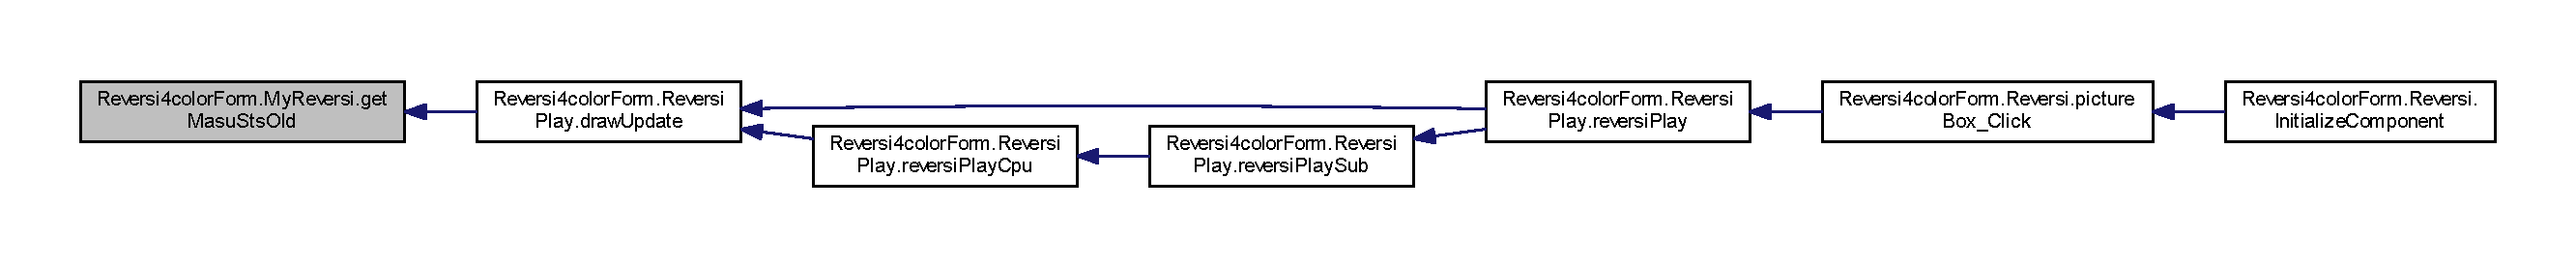
\includegraphics[width=350pt]{class_reversi4color_form_1_1_my_reversi_aa56088eff96a48e68d4c7f688fe06b8d_icgraph}
\end{center}
\end{figure}
\mbox{\Hypertarget{class_reversi4color_form_1_1_my_reversi_accf9e5107a9e029db4f4ba2968800d44}\label{class_reversi4color_form_1_1_my_reversi_accf9e5107a9e029db4f4ba2968800d44}} 
\index{Reversi4color\+Form\+::\+My\+Reversi@{Reversi4color\+Form\+::\+My\+Reversi}!get\+Pass\+Ena@{get\+Pass\+Ena}}
\index{get\+Pass\+Ena@{get\+Pass\+Ena}!Reversi4color\+Form\+::\+My\+Reversi@{Reversi4color\+Form\+::\+My\+Reversi}}
\subsubsection{\texorpdfstring{get\+Pass\+Ena()}{getPassEna()}}
{\footnotesize\ttfamily int Reversi4color\+Form.\+My\+Reversi.\+get\+Pass\+Ena (\begin{DoxyParamCaption}\item[{int}]{color,  }\item[{int}]{y,  }\item[{int}]{x }\end{DoxyParamCaption})}



パス判定 


\begin{DoxyParams}[1]{Parameters}
\mbox{\tt in}  & {\em int} & color コマ色 \\
\hline
\mbox{\tt in}  & {\em int} & y マスの\+Y座標 \\
\hline
\mbox{\tt in}  & {\em int} & x マスの\+X座標 \\
\hline
\end{DoxyParams}
\begin{DoxyReturn}{Returns}
パス判定
\begin{DoxyItemize}
\item 0 \+: N\+OT P\+A\+SS
\item 1 \+: P\+A\+SS
\end{DoxyItemize}
\end{DoxyReturn}
\begin{DoxyAuthor}{Author}
Yuta Yoshinaga 
\end{DoxyAuthor}
\begin{DoxyDate}{Date}
2017.\+10.\+20 
\end{DoxyDate}


Definition at line 1945 of file My\+Reversi.\+cs.



Referenced by Reversi4color\+Form.\+Reversi\+Play.\+reversi\+Play\+Cpu().

Here is the call graph for this function\+:\nopagebreak
\begin{figure}[H]
\begin{center}
\leavevmode
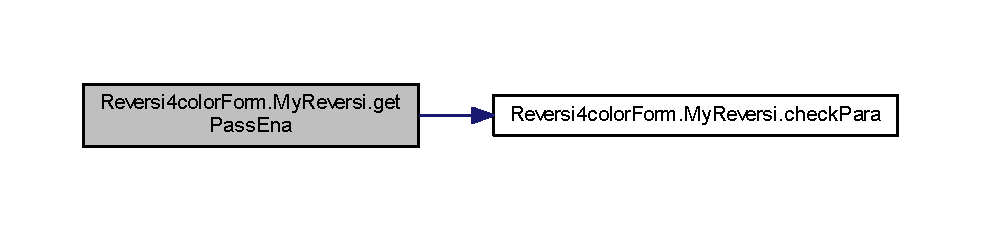
\includegraphics[width=350pt]{class_reversi4color_form_1_1_my_reversi_accf9e5107a9e029db4f4ba2968800d44_cgraph}
\end{center}
\end{figure}
Here is the caller graph for this function\+:\nopagebreak
\begin{figure}[H]
\begin{center}
\leavevmode
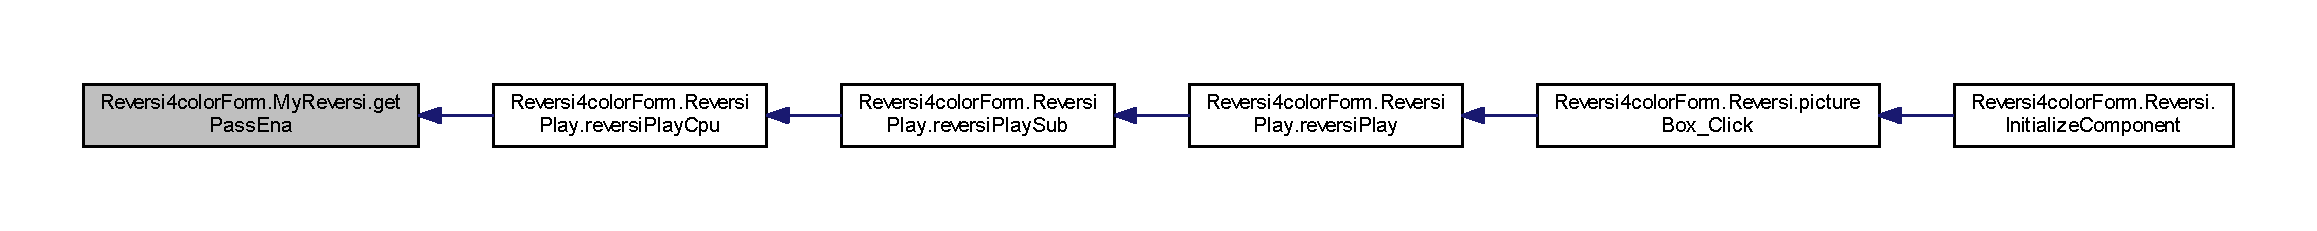
\includegraphics[width=350pt]{class_reversi4color_form_1_1_my_reversi_accf9e5107a9e029db4f4ba2968800d44_icgraph}
\end{center}
\end{figure}
\mbox{\Hypertarget{class_reversi4color_form_1_1_my_reversi_a5af52fd8272221e7fecfc8375a9f7be2}\label{class_reversi4color_form_1_1_my_reversi_a5af52fd8272221e7fecfc8375a9f7be2}} 
\index{Reversi4color\+Form\+::\+My\+Reversi@{Reversi4color\+Form\+::\+My\+Reversi}!get\+Point@{get\+Point}}
\index{get\+Point@{get\+Point}!Reversi4color\+Form\+::\+My\+Reversi@{Reversi4color\+Form\+::\+My\+Reversi}}
\subsubsection{\texorpdfstring{get\+Point()}{getPoint()}}
{\footnotesize\ttfamily \hyperlink{class_reversi4color_form_1_1_reversi_point}{Reversi\+Point} Reversi4color\+Form.\+My\+Reversi.\+get\+Point (\begin{DoxyParamCaption}\item[{int}]{color,  }\item[{int}]{num }\end{DoxyParamCaption})}



ポイント座標取得 


\begin{DoxyParams}[1]{Parameters}
\mbox{\tt in}  & {\em int} & color コマ色 \\
\hline
\mbox{\tt in}  & {\em int} & num ポイント \\
\hline
\end{DoxyParams}
\begin{DoxyReturn}{Returns}
ポイント座標 null \+: 失敗 
\end{DoxyReturn}
\begin{DoxyAuthor}{Author}
Yuta Yoshinaga 
\end{DoxyAuthor}
\begin{DoxyDate}{Date}
2017.\+10.\+20 
\end{DoxyDate}


Definition at line 1881 of file My\+Reversi.\+cs.



Referenced by Reversi4color\+Form.\+Reversi\+Play.\+reset(), and Reversi4color\+Form.\+Reversi\+Play.\+reversi\+Play\+Cpu().

Here is the call graph for this function\+:\nopagebreak
\begin{figure}[H]
\begin{center}
\leavevmode
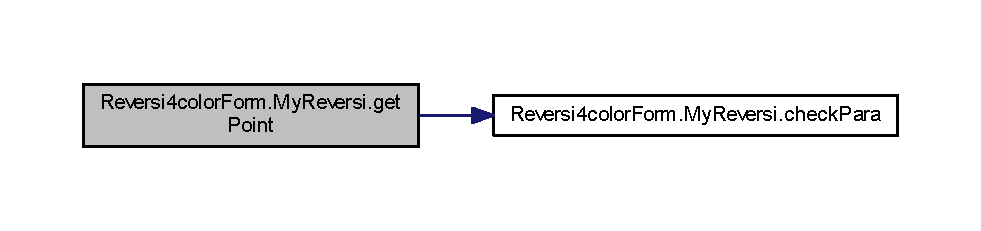
\includegraphics[width=350pt]{class_reversi4color_form_1_1_my_reversi_a5af52fd8272221e7fecfc8375a9f7be2_cgraph}
\end{center}
\end{figure}
Here is the caller graph for this function\+:\nopagebreak
\begin{figure}[H]
\begin{center}
\leavevmode
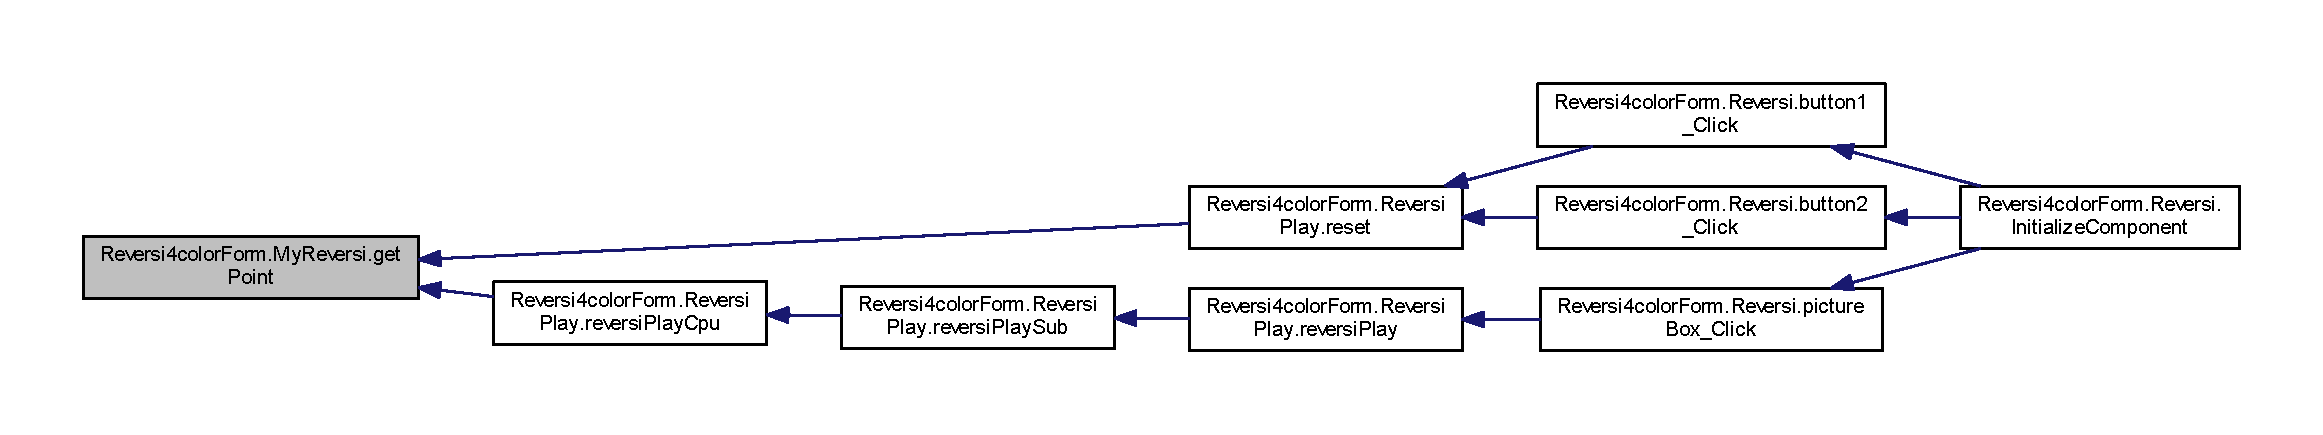
\includegraphics[width=350pt]{class_reversi4color_form_1_1_my_reversi_a5af52fd8272221e7fecfc8375a9f7be2_icgraph}
\end{center}
\end{figure}
\mbox{\Hypertarget{class_reversi4color_form_1_1_my_reversi_ad0027ead546dfa8a7844e54fb0dddfab}\label{class_reversi4color_form_1_1_my_reversi_ad0027ead546dfa8a7844e54fb0dddfab}} 
\index{Reversi4color\+Form\+::\+My\+Reversi@{Reversi4color\+Form\+::\+My\+Reversi}!get\+Point\+Anz@{get\+Point\+Anz}}
\index{get\+Point\+Anz@{get\+Point\+Anz}!Reversi4color\+Form\+::\+My\+Reversi@{Reversi4color\+Form\+::\+My\+Reversi}}
\subsubsection{\texorpdfstring{get\+Point\+Anz()}{getPointAnz()}}
{\footnotesize\ttfamily \hyperlink{class_reversi4color_form_1_1_reversi_anz}{Reversi\+Anz} Reversi4color\+Form.\+My\+Reversi.\+get\+Point\+Anz (\begin{DoxyParamCaption}\item[{int}]{color,  }\item[{int}]{y,  }\item[{int}]{x }\end{DoxyParamCaption})}



ポイント座標解析取得 


\begin{DoxyParams}[1]{Parameters}
\mbox{\tt in}  & {\em int} & color コマ色 \\
\hline
\mbox{\tt in}  & {\em int} & y マスの\+Y座標 \\
\hline
\mbox{\tt in}  & {\em int} & x マスの\+X座標 \\
\hline
\end{DoxyParams}
\begin{DoxyReturn}{Returns}
ポイント座標解析 null \+: 失敗 
\end{DoxyReturn}
\begin{DoxyAuthor}{Author}
Yuta Yoshinaga 
\end{DoxyAuthor}
\begin{DoxyDate}{Date}
2017.\+10.\+20 
\end{DoxyDate}


Definition at line 2001 of file My\+Reversi.\+cs.



Referenced by Reversi4color\+Form.\+Reversi\+Play.\+reversi\+Play\+Cpu().

Here is the call graph for this function\+:\nopagebreak
\begin{figure}[H]
\begin{center}
\leavevmode
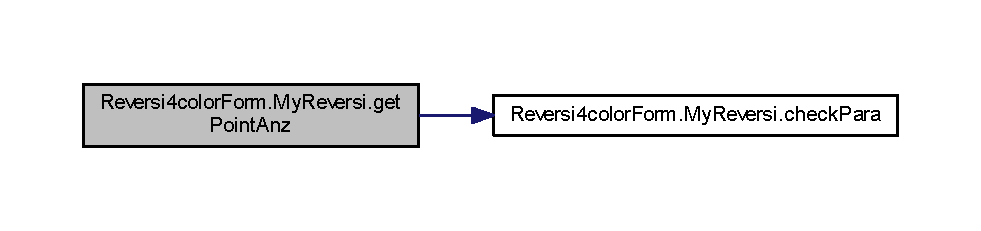
\includegraphics[width=350pt]{class_reversi4color_form_1_1_my_reversi_ad0027ead546dfa8a7844e54fb0dddfab_cgraph}
\end{center}
\end{figure}
Here is the caller graph for this function\+:\nopagebreak
\begin{figure}[H]
\begin{center}
\leavevmode
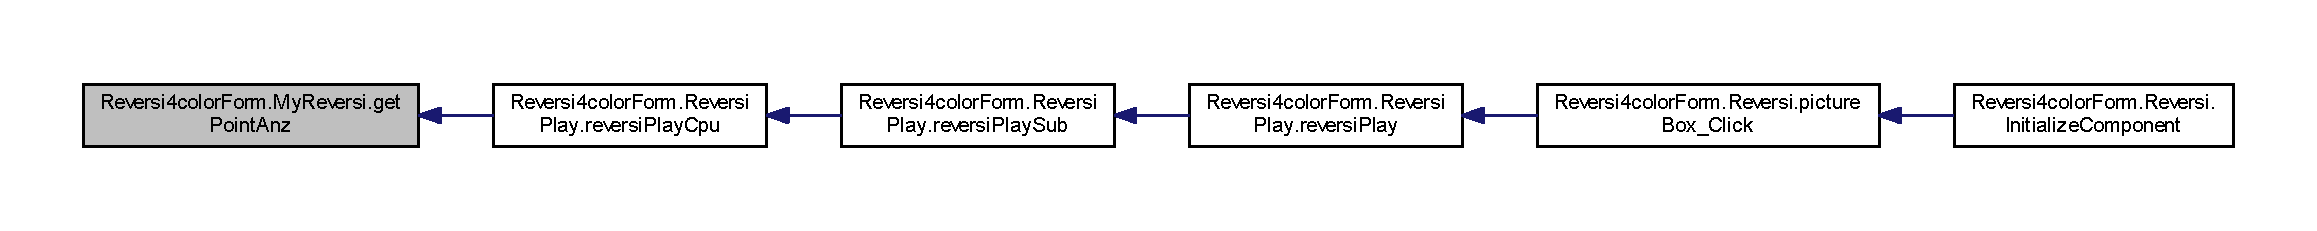
\includegraphics[width=350pt]{class_reversi4color_form_1_1_my_reversi_ad0027ead546dfa8a7844e54fb0dddfab_icgraph}
\end{center}
\end{figure}
\mbox{\Hypertarget{class_reversi4color_form_1_1_my_reversi_a64db9e5d07901c13e985e1730816bb25}\label{class_reversi4color_form_1_1_my_reversi_a64db9e5d07901c13e985e1730816bb25}} 
\index{Reversi4color\+Form\+::\+My\+Reversi@{Reversi4color\+Form\+::\+My\+Reversi}!get\+Point\+Cnt@{get\+Point\+Cnt}}
\index{get\+Point\+Cnt@{get\+Point\+Cnt}!Reversi4color\+Form\+::\+My\+Reversi@{Reversi4color\+Form\+::\+My\+Reversi}}
\subsubsection{\texorpdfstring{get\+Point\+Cnt()}{getPointCnt()}}
{\footnotesize\ttfamily int Reversi4color\+Form.\+My\+Reversi.\+get\+Point\+Cnt (\begin{DoxyParamCaption}\item[{int}]{color }\end{DoxyParamCaption})}



ポイント座標数取得 


\begin{DoxyParams}[1]{Parameters}
\mbox{\tt in}  & {\em int} & color コマ色 \\
\hline
\end{DoxyParams}
\begin{DoxyReturn}{Returns}
ポイント座標数取得 
\end{DoxyReturn}
\begin{DoxyAuthor}{Author}
Yuta Yoshinaga 
\end{DoxyAuthor}
\begin{DoxyDate}{Date}
2017.\+10.\+20 
\end{DoxyDate}


Definition at line 1902 of file My\+Reversi.\+cs.



Referenced by Reversi4color\+Form.\+My\+Reversi.\+Analysis\+Reversi\+Black(), Reversi4color\+Form.\+My\+Reversi.\+Analysis\+Reversi\+Blue(), Reversi4color\+Form.\+My\+Reversi.\+Analysis\+Reversi\+Red(), Reversi4color\+Form.\+My\+Reversi.\+Analysis\+Reversi\+White(), Reversi4color\+Form.\+Reversi\+Play.\+reset(), and Reversi4color\+Form.\+Reversi\+Play.\+reversi\+Play\+Cpu().

Here is the caller graph for this function\+:\nopagebreak
\begin{figure}[H]
\begin{center}
\leavevmode
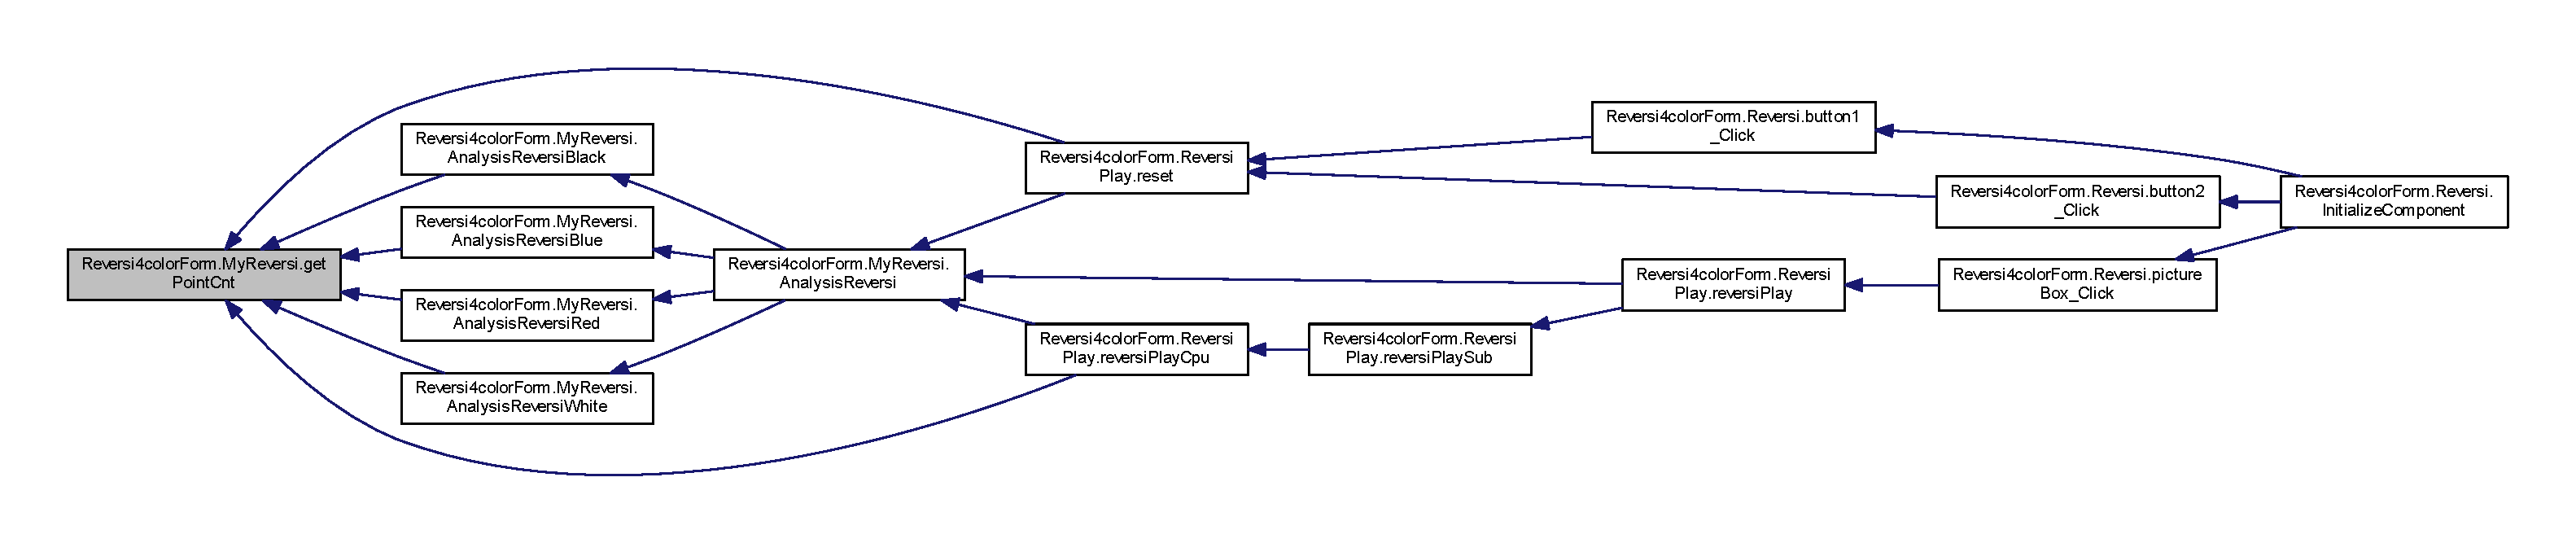
\includegraphics[width=350pt]{class_reversi4color_form_1_1_my_reversi_a64db9e5d07901c13e985e1730816bb25_icgraph}
\end{center}
\end{figure}
\mbox{\Hypertarget{class_reversi4color_form_1_1_my_reversi_afdfd5f0fc3a4ed4e24bcf67ead0bb980}\label{class_reversi4color_form_1_1_my_reversi_afdfd5f0fc3a4ed4e24bcf67ead0bb980}} 
\index{Reversi4color\+Form\+::\+My\+Reversi@{Reversi4color\+Form\+::\+My\+Reversi}!make\+Masu\+Sts@{make\+Masu\+Sts}}
\index{make\+Masu\+Sts@{make\+Masu\+Sts}!Reversi4color\+Form\+::\+My\+Reversi@{Reversi4color\+Form\+::\+My\+Reversi}}
\subsubsection{\texorpdfstring{make\+Masu\+Sts()}{makeMasuSts()}}
{\footnotesize\ttfamily int Reversi4color\+Form.\+My\+Reversi.\+make\+Masu\+Sts (\begin{DoxyParamCaption}\item[{int}]{color }\end{DoxyParamCaption})\hspace{0.3cm}{\ttfamily [private]}}



各コマの置ける場所等のステータス作成 


\begin{DoxyParams}[1]{Parameters}
\mbox{\tt in}  & {\em int} & color ステータスを作成するコマ \\
\hline
\end{DoxyParams}
\begin{DoxyReturn}{Returns}
ありません 
\end{DoxyReturn}
\begin{DoxyAuthor}{Author}
Yuta Yoshinaga 
\end{DoxyAuthor}
\begin{DoxyDate}{Date}
2017.\+10.\+20 
\end{DoxyDate}


Definition at line 407 of file My\+Reversi.\+cs.



Referenced by Reversi4color\+Form.\+My\+Reversi.\+Analysis\+Reversi(), Reversi4color\+Form.\+My\+Reversi.\+Analysis\+Reversi\+Black(), Reversi4color\+Form.\+My\+Reversi.\+Analysis\+Reversi\+Blue(), Reversi4color\+Form.\+My\+Reversi.\+Analysis\+Reversi\+Red(), Reversi4color\+Form.\+My\+Reversi.\+Analysis\+Reversi\+White(), Reversi4color\+Form.\+My\+Reversi.\+reset(), and Reversi4color\+Form.\+My\+Reversi.\+set\+Masu\+Sts().

Here is the caller graph for this function\+:\nopagebreak
\begin{figure}[H]
\begin{center}
\leavevmode
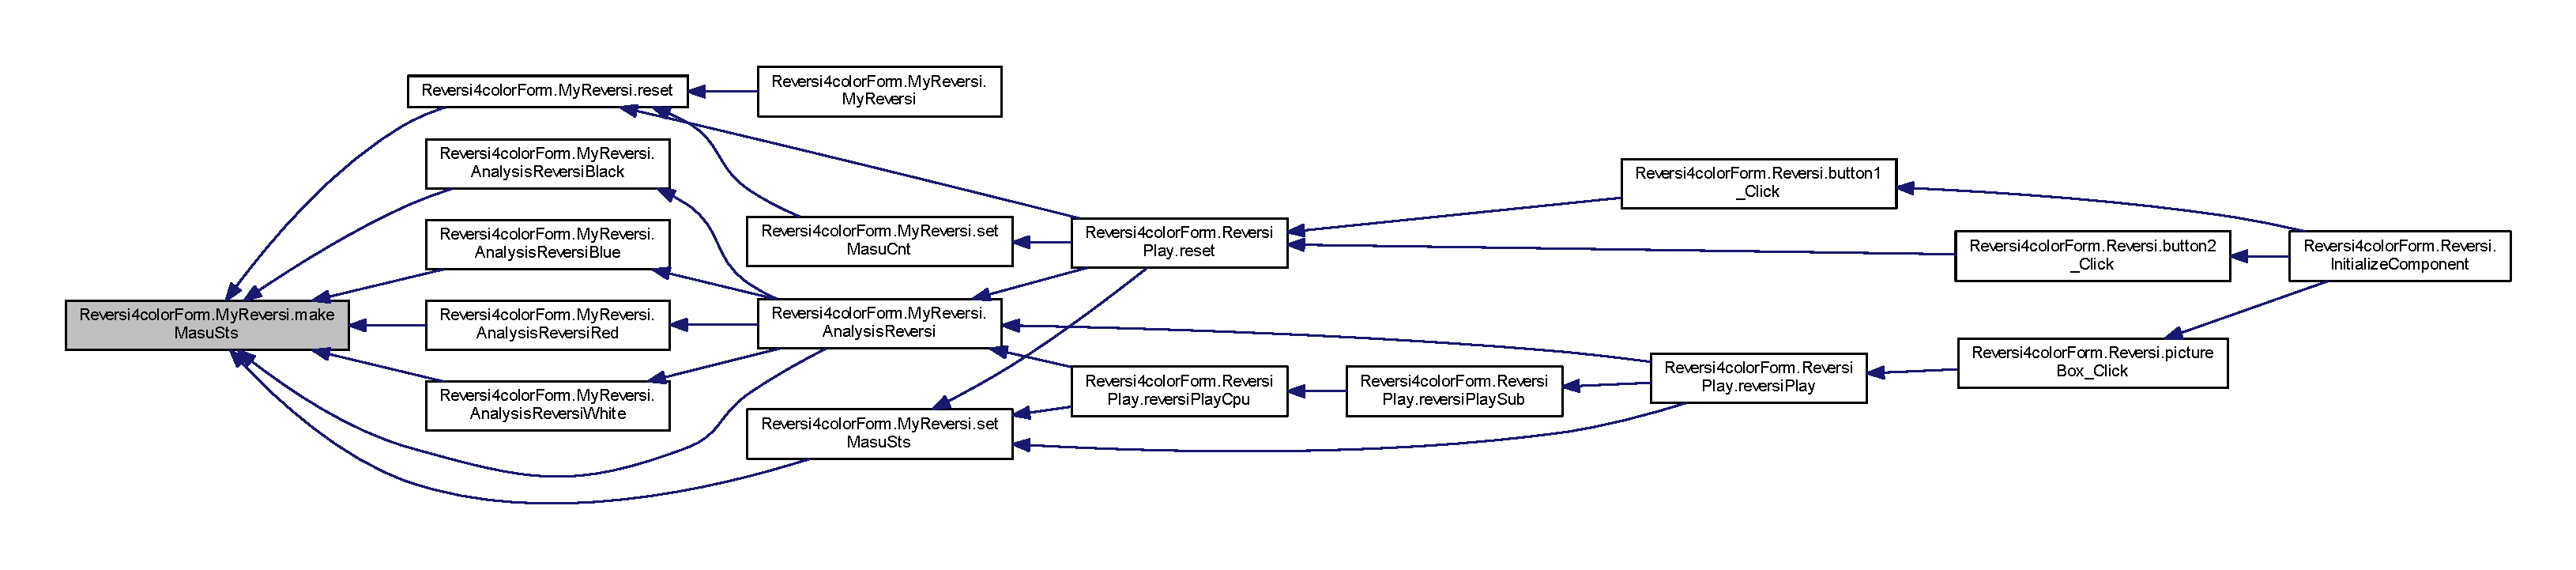
\includegraphics[width=350pt]{class_reversi4color_form_1_1_my_reversi_afdfd5f0fc3a4ed4e24bcf67ead0bb980_icgraph}
\end{center}
\end{figure}
\mbox{\Hypertarget{class_reversi4color_form_1_1_my_reversi_aeb24b855c540f99c901de08b11af1dd6}\label{class_reversi4color_form_1_1_my_reversi_aeb24b855c540f99c901de08b11af1dd6}} 
\index{Reversi4color\+Form\+::\+My\+Reversi@{Reversi4color\+Form\+::\+My\+Reversi}!reset@{reset}}
\index{reset@{reset}!Reversi4color\+Form\+::\+My\+Reversi@{Reversi4color\+Form\+::\+My\+Reversi}}
\subsubsection{\texorpdfstring{reset()}{reset()}}
{\footnotesize\ttfamily void Reversi4color\+Form.\+My\+Reversi.\+reset (\begin{DoxyParamCaption}{ }\end{DoxyParamCaption})}



リセット 

\begin{DoxyReturn}{Returns}
ありません 
\end{DoxyReturn}
\begin{DoxyAuthor}{Author}
Yuta Yoshinaga 
\end{DoxyAuthor}
\begin{DoxyDate}{Date}
2017.\+10.\+20 
\end{DoxyDate}


Definition at line 355 of file My\+Reversi.\+cs.



Referenced by Reversi4color\+Form.\+My\+Reversi.\+My\+Reversi(), Reversi4color\+Form.\+Reversi\+Play.\+reset(), and Reversi4color\+Form.\+My\+Reversi.\+set\+Masu\+Cnt().

Here is the call graph for this function\+:\nopagebreak
\begin{figure}[H]
\begin{center}
\leavevmode
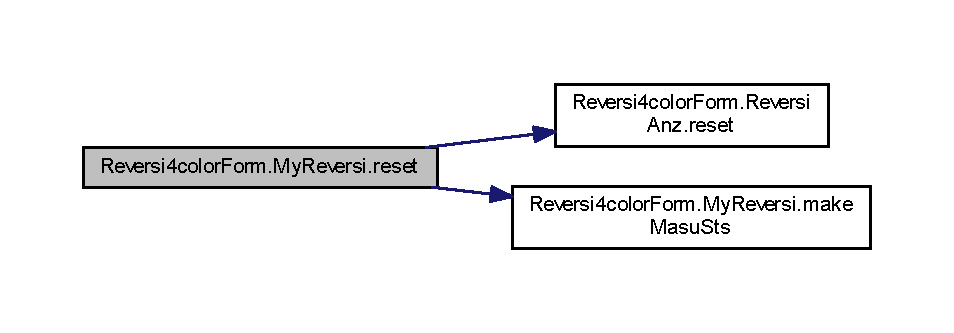
\includegraphics[width=350pt]{class_reversi4color_form_1_1_my_reversi_aeb24b855c540f99c901de08b11af1dd6_cgraph}
\end{center}
\end{figure}
Here is the caller graph for this function\+:\nopagebreak
\begin{figure}[H]
\begin{center}
\leavevmode
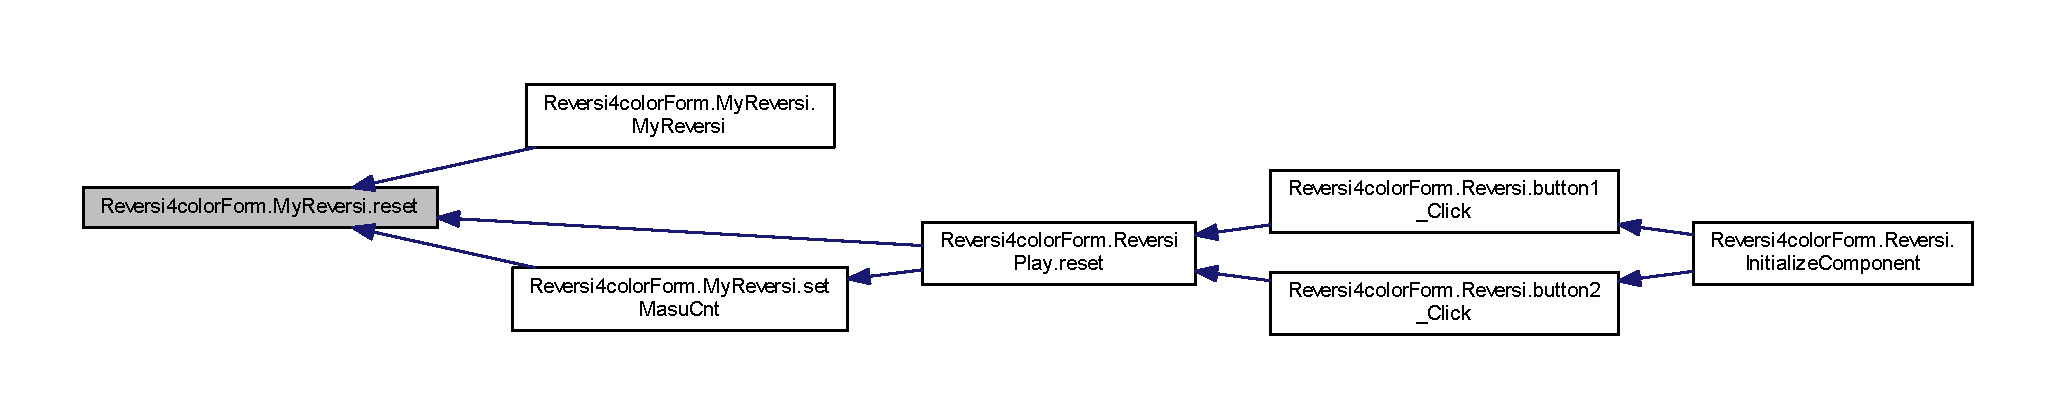
\includegraphics[width=350pt]{class_reversi4color_form_1_1_my_reversi_aeb24b855c540f99c901de08b11af1dd6_icgraph}
\end{center}
\end{figure}
\mbox{\Hypertarget{class_reversi4color_form_1_1_my_reversi_a94536b8feaa37ca51b3d0612befae12f}\label{class_reversi4color_form_1_1_my_reversi_a94536b8feaa37ca51b3d0612befae12f}} 
\index{Reversi4color\+Form\+::\+My\+Reversi@{Reversi4color\+Form\+::\+My\+Reversi}!rev\+Masu\+Sts@{rev\+Masu\+Sts}}
\index{rev\+Masu\+Sts@{rev\+Masu\+Sts}!Reversi4color\+Form\+::\+My\+Reversi@{Reversi4color\+Form\+::\+My\+Reversi}}
\subsubsection{\texorpdfstring{rev\+Masu\+Sts()}{revMasuSts()}}
{\footnotesize\ttfamily void Reversi4color\+Form.\+My\+Reversi.\+rev\+Masu\+Sts (\begin{DoxyParamCaption}\item[{int}]{color,  }\item[{int}]{y,  }\item[{int}]{x }\end{DoxyParamCaption})\hspace{0.3cm}{\ttfamily [private]}}



コマをひっくり返す 


\begin{DoxyParams}[1]{Parameters}
\mbox{\tt in}  & {\em int} & color ひっくり返す元コマ \\
\hline
\mbox{\tt in}  & {\em int} & y ひっくり返す元コマの\+Y座標 \\
\hline
\mbox{\tt in}  & {\em int} & x ひっくり返す元コマの\+X座標 \\
\hline
\end{DoxyParams}
\begin{DoxyReturn}{Returns}
ありません 
\end{DoxyReturn}
\begin{DoxyAuthor}{Author}
Yuta Yoshinaga 
\end{DoxyAuthor}
\begin{DoxyDate}{Date}
2017.\+10.\+20 
\end{DoxyDate}


Definition at line 657 of file My\+Reversi.\+cs.



Referenced by Reversi4color\+Form.\+My\+Reversi.\+Analysis\+Reversi\+Black(), Reversi4color\+Form.\+My\+Reversi.\+Analysis\+Reversi\+Blue(), Reversi4color\+Form.\+My\+Reversi.\+Analysis\+Reversi\+Red(), Reversi4color\+Form.\+My\+Reversi.\+Analysis\+Reversi\+White(), and Reversi4color\+Form.\+My\+Reversi.\+set\+Masu\+Sts().

Here is the caller graph for this function\+:\nopagebreak
\begin{figure}[H]
\begin{center}
\leavevmode
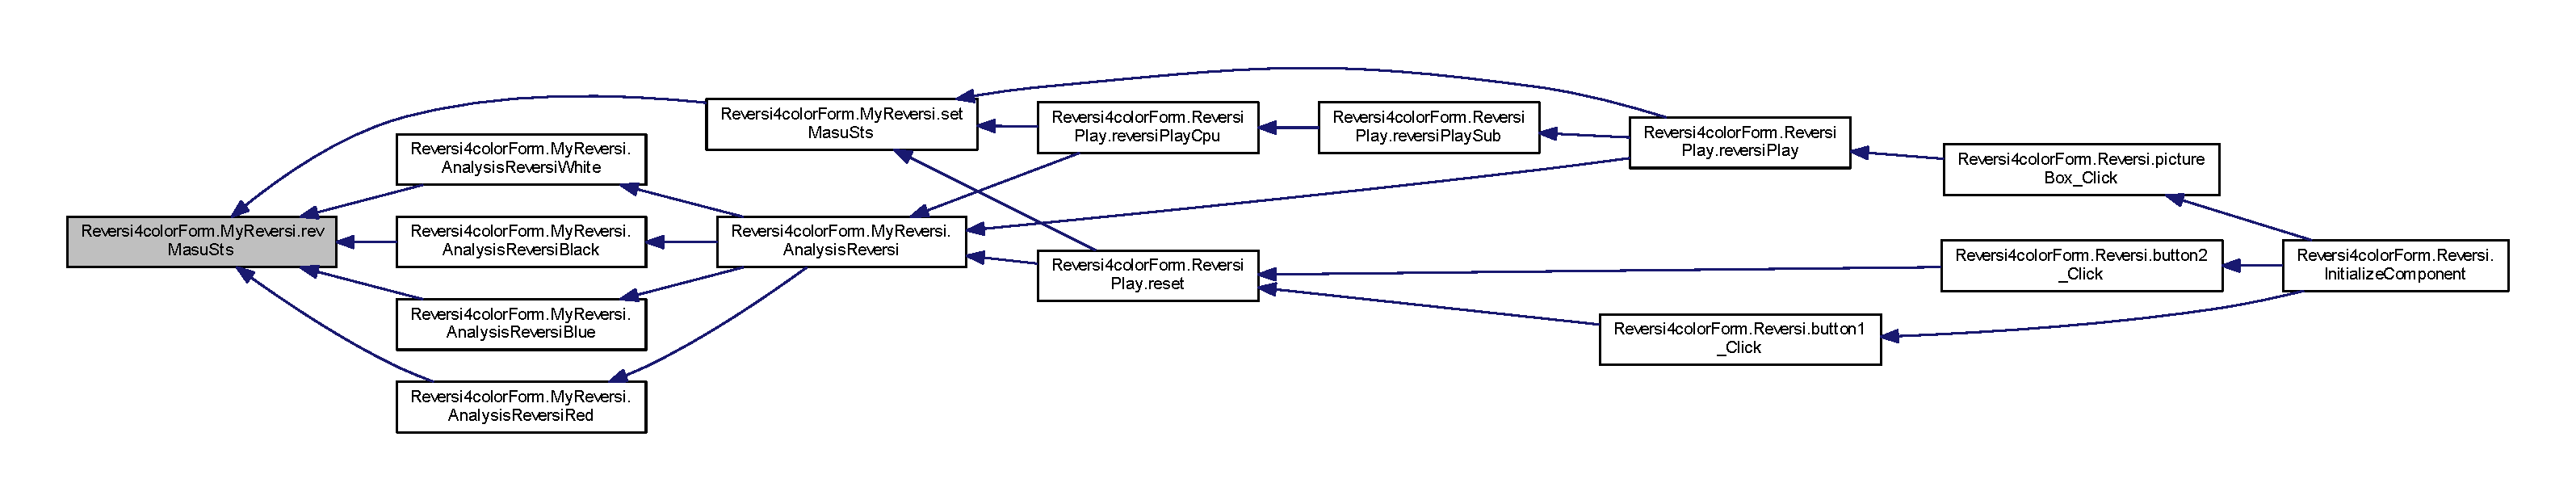
\includegraphics[width=350pt]{class_reversi4color_form_1_1_my_reversi_a94536b8feaa37ca51b3d0612befae12f_icgraph}
\end{center}
\end{figure}
\mbox{\Hypertarget{class_reversi4color_form_1_1_my_reversi_ae612bc1a7a5ccbd972ce130de910e8e6}\label{class_reversi4color_form_1_1_my_reversi_ae612bc1a7a5ccbd972ce130de910e8e6}} 
\index{Reversi4color\+Form\+::\+My\+Reversi@{Reversi4color\+Form\+::\+My\+Reversi}!set\+Masu\+Cnt@{set\+Masu\+Cnt}}
\index{set\+Masu\+Cnt@{set\+Masu\+Cnt}!Reversi4color\+Form\+::\+My\+Reversi@{Reversi4color\+Form\+::\+My\+Reversi}}
\subsubsection{\texorpdfstring{set\+Masu\+Cnt()}{setMasuCnt()}}
{\footnotesize\ttfamily int Reversi4color\+Form.\+My\+Reversi.\+set\+Masu\+Cnt (\begin{DoxyParamCaption}\item[{int}]{cnt }\end{DoxyParamCaption})}



マスの数変更 


\begin{DoxyParams}[1]{Parameters}
\mbox{\tt in}  & {\em int} & cnt マスの数 \\
\hline
\end{DoxyParams}
\begin{DoxyReturn}{Returns}
0 \+: 成功 それ以外 \+: 失敗 
\end{DoxyReturn}
\begin{DoxyAuthor}{Author}
Yuta Yoshinaga 
\end{DoxyAuthor}
\begin{DoxyDate}{Date}
2017.\+10.\+20 
\end{DoxyDate}


Definition at line 1856 of file My\+Reversi.\+cs.



Referenced by Reversi4color\+Form.\+Reversi\+Play.\+reset().

Here is the call graph for this function\+:\nopagebreak
\begin{figure}[H]
\begin{center}
\leavevmode
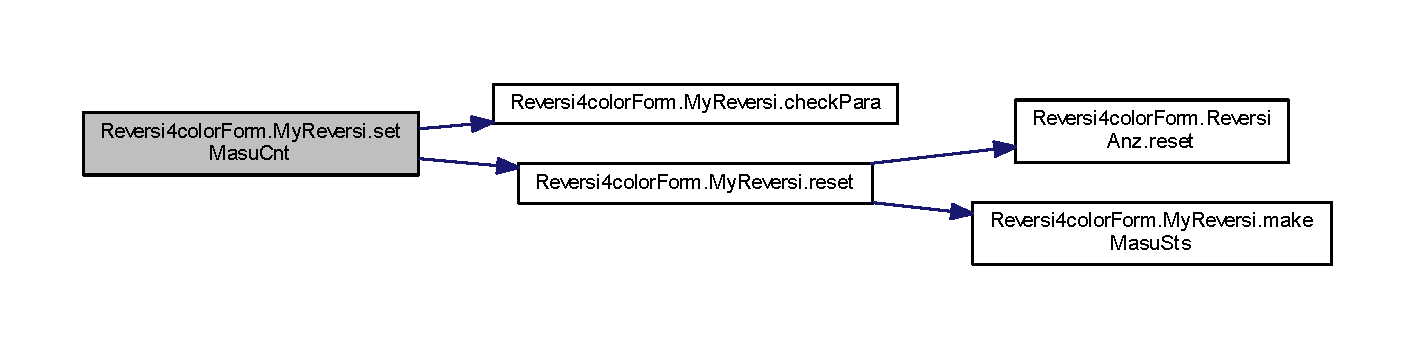
\includegraphics[width=350pt]{class_reversi4color_form_1_1_my_reversi_ae612bc1a7a5ccbd972ce130de910e8e6_cgraph}
\end{center}
\end{figure}
Here is the caller graph for this function\+:\nopagebreak
\begin{figure}[H]
\begin{center}
\leavevmode
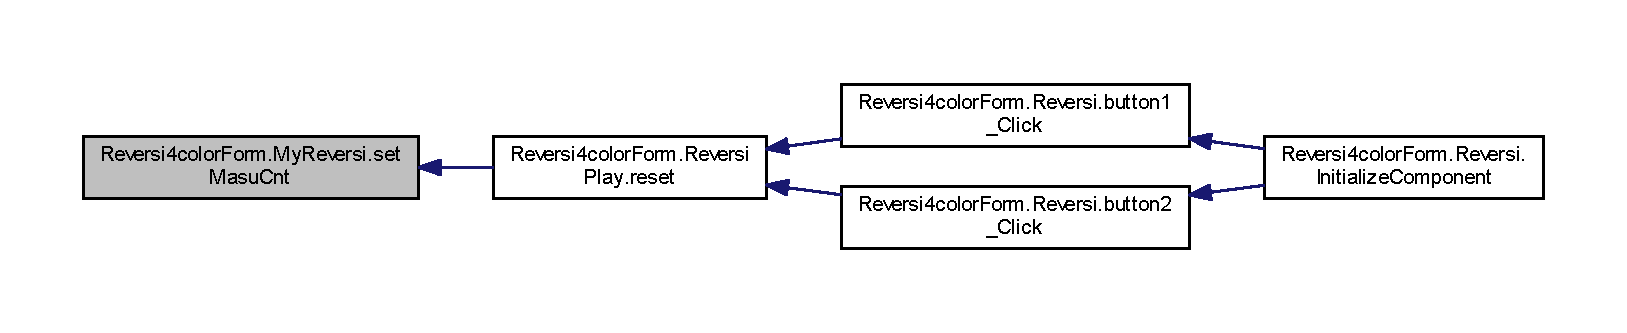
\includegraphics[width=350pt]{class_reversi4color_form_1_1_my_reversi_ae612bc1a7a5ccbd972ce130de910e8e6_icgraph}
\end{center}
\end{figure}
\mbox{\Hypertarget{class_reversi4color_form_1_1_my_reversi_a7b7f5f6c8ea7961a41cb3dcc4360c9d1}\label{class_reversi4color_form_1_1_my_reversi_a7b7f5f6c8ea7961a41cb3dcc4360c9d1}} 
\index{Reversi4color\+Form\+::\+My\+Reversi@{Reversi4color\+Form\+::\+My\+Reversi}!set\+Masu\+Sts@{set\+Masu\+Sts}}
\index{set\+Masu\+Sts@{set\+Masu\+Sts}!Reversi4color\+Form\+::\+My\+Reversi@{Reversi4color\+Form\+::\+My\+Reversi}}
\subsubsection{\texorpdfstring{set\+Masu\+Sts()}{setMasuSts()}}
{\footnotesize\ttfamily int Reversi4color\+Form.\+My\+Reversi.\+set\+Masu\+Sts (\begin{DoxyParamCaption}\item[{int}]{color,  }\item[{int}]{y,  }\item[{int}]{x }\end{DoxyParamCaption})}



指定座標にコマを置く 


\begin{DoxyParams}[1]{Parameters}
\mbox{\tt in}  & {\em int} & color コマ色 \\
\hline
\mbox{\tt in}  & {\em int} & y マスの\+Y座標 \\
\hline
\mbox{\tt in}  & {\em int} & x マスの\+X座標 \\
\hline
\end{DoxyParams}
\begin{DoxyReturn}{Returns}
0 \+: 成功 それ以外 \+: 失敗 
\end{DoxyReturn}
\begin{DoxyAuthor}{Author}
Yuta Yoshinaga 
\end{DoxyAuthor}
\begin{DoxyDate}{Date}
2017.\+10.\+20 
\end{DoxyDate}


Definition at line 1804 of file My\+Reversi.\+cs.



Referenced by Reversi4color\+Form.\+Reversi\+Play.\+reset(), Reversi4color\+Form.\+Reversi\+Play.\+reversi\+Play(), and Reversi4color\+Form.\+Reversi\+Play.\+reversi\+Play\+Cpu().

Here is the call graph for this function\+:\nopagebreak
\begin{figure}[H]
\begin{center}
\leavevmode
\includegraphics[width=350pt]{class_reversi4color_form_1_1_my_reversi_a7b7f5f6c8ea7961a41cb3dcc4360c9d1_cgraph}
\end{center}
\end{figure}
Here is the caller graph for this function\+:\nopagebreak
\begin{figure}[H]
\begin{center}
\leavevmode
\includegraphics[width=350pt]{class_reversi4color_form_1_1_my_reversi_a7b7f5f6c8ea7961a41cb3dcc4360c9d1_icgraph}
\end{center}
\end{figure}
\mbox{\Hypertarget{class_reversi4color_form_1_1_my_reversi_a099e2baa5bcf58eeeb0fe1cbe8be94d7}\label{class_reversi4color_form_1_1_my_reversi_a099e2baa5bcf58eeeb0fe1cbe8be94d7}} 
\index{Reversi4color\+Form\+::\+My\+Reversi@{Reversi4color\+Form\+::\+My\+Reversi}!set\+Masu\+Sts\+Forcibly@{set\+Masu\+Sts\+Forcibly}}
\index{set\+Masu\+Sts\+Forcibly@{set\+Masu\+Sts\+Forcibly}!Reversi4color\+Form\+::\+My\+Reversi@{Reversi4color\+Form\+::\+My\+Reversi}}
\subsubsection{\texorpdfstring{set\+Masu\+Sts\+Forcibly()}{setMasuStsForcibly()}}
{\footnotesize\ttfamily int Reversi4color\+Form.\+My\+Reversi.\+set\+Masu\+Sts\+Forcibly (\begin{DoxyParamCaption}\item[{int}]{color,  }\item[{int}]{y,  }\item[{int}]{x }\end{DoxyParamCaption})}



指定座標にコマを強制的に置く 


\begin{DoxyParams}[1]{Parameters}
\mbox{\tt in}  & {\em int} & color コマ色 \\
\hline
\mbox{\tt in}  & {\em int} & y マスの\+Y座標 \\
\hline
\mbox{\tt in}  & {\em int} & x マスの\+X座標 \\
\hline
\end{DoxyParams}
\begin{DoxyReturn}{Returns}
0 \+: 成功 それ以外 \+: 失敗 
\end{DoxyReturn}
\begin{DoxyAuthor}{Author}
Yuta Yoshinaga 
\end{DoxyAuthor}
\begin{DoxyDate}{Date}
2017.\+10.\+20 
\end{DoxyDate}


Definition at line 1838 of file My\+Reversi.\+cs.



Referenced by Reversi4color\+Form.\+Reversi\+Play.\+game\+End\+Anim\+Exec().

Here is the caller graph for this function\+:\nopagebreak
\begin{figure}[H]
\begin{center}
\leavevmode
\includegraphics[width=350pt]{class_reversi4color_form_1_1_my_reversi_a099e2baa5bcf58eeeb0fe1cbe8be94d7_icgraph}
\end{center}
\end{figure}


The documentation for this class was generated from the following file\+:\begin{DoxyCompactItemize}
\item 
Model/\hyperlink{_my_reversi_8cs}{My\+Reversi.\+cs}\end{DoxyCompactItemize}

\hypertarget{class_reversi4color_form_1_1_program}{}\section{Reversi4color\+Form.\+Program Class Reference}
\label{class_reversi4color_form_1_1_program}\index{Reversi4color\+Form.\+Program@{Reversi4color\+Form.\+Program}}


Collaboration diagram for Reversi4color\+Form.\+Program\+:
\nopagebreak
\begin{figure}[H]
\begin{center}
\leavevmode
\includegraphics[width=217pt]{class_reversi4color_form_1_1_program__coll__graph}
\end{center}
\end{figure}
\subsection*{Static Private Member Functions}
\begin{DoxyCompactItemize}
\item 
static void \hyperlink{class_reversi4color_form_1_1_program_a2edae1f309199d01d6561ca9f1b09454}{Main} ()
\begin{DoxyCompactList}\small\item\em アプリケーションのメイン エントリ ポイントです。 \end{DoxyCompactList}\end{DoxyCompactItemize}


\subsection{Detailed Description}


Definition at line 9 of file Program.\+cs.



\subsection{Member Function Documentation}
\mbox{\Hypertarget{class_reversi4color_form_1_1_program_a2edae1f309199d01d6561ca9f1b09454}\label{class_reversi4color_form_1_1_program_a2edae1f309199d01d6561ca9f1b09454}} 
\index{Reversi4color\+Form\+::\+Program@{Reversi4color\+Form\+::\+Program}!Main@{Main}}
\index{Main@{Main}!Reversi4color\+Form\+::\+Program@{Reversi4color\+Form\+::\+Program}}
\subsubsection{\texorpdfstring{Main()}{Main()}}
{\footnotesize\ttfamily static void Reversi4color\+Form.\+Program.\+Main (\begin{DoxyParamCaption}{ }\end{DoxyParamCaption})\hspace{0.3cm}{\ttfamily [static]}, {\ttfamily [private]}}



アプリケーションのメイン エントリ ポイントです。 



Definition at line 15 of file Program.\+cs.



The documentation for this class was generated from the following file\+:\begin{DoxyCompactItemize}
\item 
Program.\+cs\end{DoxyCompactItemize}

\hypertarget{class_reversi4color_form_1_1_reversi}{}\section{Reversi4color\+Form.\+Reversi Class Reference}
\label{class_reversi4color_form_1_1_reversi}\index{Reversi4color\+Form.\+Reversi@{Reversi4color\+Form.\+Reversi}}


Inheritance diagram for Reversi4color\+Form.\+Reversi\+:
\nopagebreak
\begin{figure}[H]
\begin{center}
\leavevmode
\includegraphics[height=550pt]{class_reversi4color_form_1_1_reversi__inherit__graph}
\end{center}
\end{figure}


Collaboration diagram for Reversi4color\+Form.\+Reversi\+:
\nopagebreak
\begin{figure}[H]
\begin{center}
\leavevmode
\includegraphics[height=550pt]{class_reversi4color_form_1_1_reversi__coll__graph}
\end{center}
\end{figure}
\subsection*{Public Member Functions}
\begin{DoxyCompactItemize}
\item 
\hyperlink{class_reversi4color_form_1_1_reversi_setting}{Reversi\+Setting} \hyperlink{class_reversi4color_form_1_1_reversi_a944e9618d0eac2a6928d8a8ec835d384}{Load\+Setting\+Xml} (string path)
\begin{DoxyCompactList}\small\item\em 設定\+X\+M\+Lファイルロード \end{DoxyCompactList}\item 
int \hyperlink{class_reversi4color_form_1_1_reversi_aff9f10404fc96f56154073d324d4dea2}{Save\+Setting\+Xml} (string path, ref \hyperlink{class_reversi4color_form_1_1_reversi_setting}{Reversi\+Setting} app\+Set)
\begin{DoxyCompactList}\small\item\em 設定\+X\+M\+Lファイルセーブ \end{DoxyCompactList}\item 
void \hyperlink{class_reversi4color_form_1_1_reversi_ab30feb8c247bae6c78fa935456cf909a}{app\+Init} ()
\begin{DoxyCompactList}\small\item\em アプリ初期化 \end{DoxyCompactList}\item 
void \hyperlink{class_reversi4color_form_1_1_reversi_a4a67f1f9a3782d08790aa60b5ce10ab0}{View\+Msg\+Dlg} (string title, string msg)
\begin{DoxyCompactList}\small\item\em メッセージダイアログ \end{DoxyCompactList}\item 
void \hyperlink{class_reversi4color_form_1_1_reversi_a344c1f42605e074a5a110878a7cfe87a}{View\+Msg\+Dlg\+Local} (string title, string msg)
\begin{DoxyCompactList}\small\item\em メッセージダイアログ \end{DoxyCompactList}\item 
void \hyperlink{class_reversi4color_form_1_1_reversi_a5f463083da645873e96e605d25273357}{Draw\+Single} (int y, int x, int sts, int bk, string text)
\begin{DoxyCompactList}\small\item\em 1マス描画 \end{DoxyCompactList}\item 
void \hyperlink{class_reversi4color_form_1_1_reversi_a82fb011304d47866a85a9092fe4be6b7}{Draw\+Single\+Local} (int y, int x, int sts, int bk, string text)
\begin{DoxyCompactList}\small\item\em 1マス描画 \end{DoxyCompactList}\item 
void \hyperlink{class_reversi4color_form_1_1_reversi_acb7220a84f599ebf736216cc055b2ae3}{Cur\+Col\+Msg} (string text)
\begin{DoxyCompactList}\small\item\em 現在の色メッセージ \end{DoxyCompactList}\item 
void \hyperlink{class_reversi4color_form_1_1_reversi_a6ab2074a5474736e76644cf45c08827b}{Cur\+Col\+Msg\+Local} (string text)
\begin{DoxyCompactList}\small\item\em 現在の色メッセージ \end{DoxyCompactList}\item 
void \hyperlink{class_reversi4color_form_1_1_reversi_af82882188f72f849b21890fe21199083}{Cur\+Sts\+Msg} (string text)
\begin{DoxyCompactList}\small\item\em 現在のステータスメッセージ \end{DoxyCompactList}\item 
void \hyperlink{class_reversi4color_form_1_1_reversi_a663e1d055e099d0855df8a34af31edf9}{Cur\+Sts\+Msg\+Local} (string text)
\begin{DoxyCompactList}\small\item\em 現在のステータスメッセージ \end{DoxyCompactList}\end{DoxyCompactItemize}
\subsection*{Public Attributes}
\begin{DoxyCompactItemize}
\item 
\mbox{\Hypertarget{class_reversi4color_form_1_1_reversi_acf0a86323b8a7494bc65dcb9945e19c1}\label{class_reversi4color_form_1_1_reversi_acf0a86323b8a7494bc65dcb9945e19c1}} 
\hyperlink{class_reversi4color_form_1_1_reversi_setting}{Reversi\+Setting} \hyperlink{class_reversi4color_form_1_1_reversi_acf0a86323b8a7494bc65dcb9945e19c1}{m\+\_\+\+App\+Settings}
\begin{DoxyCompactList}\small\item\em アプリ設定 \end{DoxyCompactList}\item 
\mbox{\Hypertarget{class_reversi4color_form_1_1_reversi_ae82e78a9e55c65e5909715b5eb1ec1e1}\label{class_reversi4color_form_1_1_reversi_ae82e78a9e55c65e5909715b5eb1ec1e1}} 
\hyperlink{class_reversi4color_form_1_1_reversi_play}{Reversi\+Play} \hyperlink{class_reversi4color_form_1_1_reversi_ae82e78a9e55c65e5909715b5eb1ec1e1}{m\+\_\+\+Reversi\+Play}
\begin{DoxyCompactList}\small\item\em リバーシ本体 \end{DoxyCompactList}\end{DoxyCompactItemize}
\subsection*{Protected Member Functions}
\begin{DoxyCompactItemize}
\item 
override void \hyperlink{class_reversi4color_form_1_1_reversi_aa6fa1c8eae6d12a2e4f310ef0acddbb1}{Dispose} (bool disposing)
\begin{DoxyCompactList}\small\item\em 使用中のリソースをすべてクリーンアップします。 \end{DoxyCompactList}\end{DoxyCompactItemize}
\subsection*{Private Member Functions}
\begin{DoxyCompactItemize}
\item 
\mbox{\Hypertarget{class_reversi4color_form_1_1_reversi_aa83ab1c0d7ce3e62ff0a7621f828c605}\label{class_reversi4color_form_1_1_reversi_aa83ab1c0d7ce3e62ff0a7621f828c605}} 
delegate void {\bfseries View\+Msg\+Dlg\+Delegate} (string title, string msg)
\item 
\mbox{\Hypertarget{class_reversi4color_form_1_1_reversi_ad81ae0deeca8d7b1f8946f54e5af7602}\label{class_reversi4color_form_1_1_reversi_ad81ae0deeca8d7b1f8946f54e5af7602}} 
delegate void {\bfseries Draw\+Single\+Delegate} (int y, int x, int sts, int bk, string text)
\item 
\mbox{\Hypertarget{class_reversi4color_form_1_1_reversi_aa4d911dab2f8eb28788a16a50f2c16b7}\label{class_reversi4color_form_1_1_reversi_aa4d911dab2f8eb28788a16a50f2c16b7}} 
delegate void {\bfseries Cur\+Col\+Msg\+Delegate} (string text)
\item 
\mbox{\Hypertarget{class_reversi4color_form_1_1_reversi_ae7e6cf23f7b9ecc3b127cb0a4c6f1b11}\label{class_reversi4color_form_1_1_reversi_ae7e6cf23f7b9ecc3b127cb0a4c6f1b11}} 
delegate void {\bfseries Cur\+Sts\+Msg\+Delegate} (string text)
\item 
\mbox{\Hypertarget{class_reversi4color_form_1_1_reversi_adc77f11d95e862ea51cb3c7a3a816f99}\label{class_reversi4color_form_1_1_reversi_adc77f11d95e862ea51cb3c7a3a816f99}} 
delegate void {\bfseries Reversi\+\_\+\+Resize\+End\+Delegate} (object sender, Event\+Args e)
\item 
void \hyperlink{class_reversi4color_form_1_1_reversi_af0467d1e6e97eab2d7f6f12384129135}{picture\+Box\+\_\+\+Click} (object sender, Event\+Args e)
\begin{DoxyCompactList}\small\item\em マスクリック \end{DoxyCompactList}\item 
void \hyperlink{class_reversi4color_form_1_1_reversi_a6c7543d2823cf116c55bba3b970e4931}{button1\+\_\+\+Click} (object sender, Event\+Args e)
\begin{DoxyCompactList}\small\item\em リセットクリック \end{DoxyCompactList}\item 
void \hyperlink{class_reversi4color_form_1_1_reversi_a99a5abaa127633df40da37167d579541}{button2\+\_\+\+Click} (object sender, Event\+Args e)
\begin{DoxyCompactList}\small\item\em セッティングクリック \end{DoxyCompactList}\item 
void \hyperlink{class_reversi4color_form_1_1_reversi_afacffb0f4d383892677acfd1b7304606}{Reversi\+\_\+\+Resize} (object sender, Event\+Args e)
\begin{DoxyCompactList}\small\item\em リサイズイベント \end{DoxyCompactList}\item 
\mbox{\Hypertarget{class_reversi4color_form_1_1_reversi_ad13d5590335e33bf4be4fd98394a43eb}\label{class_reversi4color_form_1_1_reversi_ad13d5590335e33bf4be4fd98394a43eb}} 
void {\bfseries Reversi\+\_\+\+Resize\+End} (object sender, Event\+Args e)
\item 
void \hyperlink{class_reversi4color_form_1_1_reversi_a601896143334140db49faaa57b710aa6}{On\+Timed\+Event} (object source, Elapsed\+Event\+Args e)
\begin{DoxyCompactList}\small\item\em タイマーイベント \end{DoxyCompactList}\item 
void \hyperlink{class_reversi4color_form_1_1_reversi_a9eb7787e255c6aab7c75d6f0730e579e}{Initialize\+Component} ()
\begin{DoxyCompactList}\small\item\em デザイナー サポートに必要なメソッドです。このメソッドの内容を コード エディターで変更しないでください。 \end{DoxyCompactList}\end{DoxyCompactItemize}
\subsection*{Private Attributes}
\begin{DoxyCompactItemize}
\item 
\mbox{\Hypertarget{class_reversi4color_form_1_1_reversi_a2cb7872bfa8099a958c4b0442c58870c}\label{class_reversi4color_form_1_1_reversi_a2cb7872bfa8099a958c4b0442c58870c}} 
Size \hyperlink{class_reversi4color_form_1_1_reversi_a2cb7872bfa8099a958c4b0442c58870c}{old\+Size}
\begin{DoxyCompactList}\small\item\em リサイズ前のサイズ \end{DoxyCompactList}\item 
System.\+Component\+Model.\+I\+Container \hyperlink{class_reversi4color_form_1_1_reversi_aaf7b7fe6d6a976a0e1465cf6a60e7f7d}{components} = null
\begin{DoxyCompactList}\small\item\em 必要なデザイナー変数です。 \end{DoxyCompactList}\item 
\mbox{\Hypertarget{class_reversi4color_form_1_1_reversi_a7bc09c1323a35b04bdc1237345336053}\label{class_reversi4color_form_1_1_reversi_a7bc09c1323a35b04bdc1237345336053}} 
System.\+Windows.\+Forms.\+Table\+Layout\+Panel {\bfseries table\+Layout\+Panel1}
\item 
\mbox{\Hypertarget{class_reversi4color_form_1_1_reversi_a180b71b6dcbaab410c13c6b106844c5b}\label{class_reversi4color_form_1_1_reversi_a180b71b6dcbaab410c13c6b106844c5b}} 
System.\+Windows.\+Forms.\+Picture\+Box {\bfseries picture\+Box381}
\item 
\mbox{\Hypertarget{class_reversi4color_form_1_1_reversi_a72772c044e184bc0b2f65f5364ab4677}\label{class_reversi4color_form_1_1_reversi_a72772c044e184bc0b2f65f5364ab4677}} 
System.\+Windows.\+Forms.\+Picture\+Box {\bfseries picture\+Box382}
\item 
\mbox{\Hypertarget{class_reversi4color_form_1_1_reversi_aee558a3af72eaa080d5e24a17c8d72c8}\label{class_reversi4color_form_1_1_reversi_aee558a3af72eaa080d5e24a17c8d72c8}} 
System.\+Windows.\+Forms.\+Picture\+Box {\bfseries picture\+Box383}
\item 
\mbox{\Hypertarget{class_reversi4color_form_1_1_reversi_ad34f79700724b43dd8e8a4746ec38970}\label{class_reversi4color_form_1_1_reversi_ad34f79700724b43dd8e8a4746ec38970}} 
System.\+Windows.\+Forms.\+Picture\+Box {\bfseries picture\+Box384}
\item 
\mbox{\Hypertarget{class_reversi4color_form_1_1_reversi_af2ce89053caad9fa507d54adfc32832f}\label{class_reversi4color_form_1_1_reversi_af2ce89053caad9fa507d54adfc32832f}} 
System.\+Windows.\+Forms.\+Picture\+Box {\bfseries picture\+Box385}
\item 
\mbox{\Hypertarget{class_reversi4color_form_1_1_reversi_a02b91b1650cf3da67f2e817aa57b6e67}\label{class_reversi4color_form_1_1_reversi_a02b91b1650cf3da67f2e817aa57b6e67}} 
System.\+Windows.\+Forms.\+Picture\+Box {\bfseries picture\+Box386}
\item 
\mbox{\Hypertarget{class_reversi4color_form_1_1_reversi_a70eb0bbca16e0e8126d2f5e04631e19e}\label{class_reversi4color_form_1_1_reversi_a70eb0bbca16e0e8126d2f5e04631e19e}} 
System.\+Windows.\+Forms.\+Picture\+Box {\bfseries picture\+Box387}
\item 
\mbox{\Hypertarget{class_reversi4color_form_1_1_reversi_a2d1397e4f055daabd9a91e674fa69e53}\label{class_reversi4color_form_1_1_reversi_a2d1397e4f055daabd9a91e674fa69e53}} 
System.\+Windows.\+Forms.\+Picture\+Box {\bfseries picture\+Box388}
\item 
\mbox{\Hypertarget{class_reversi4color_form_1_1_reversi_ad7b4019d5495615be76ae0e49f8b66a0}\label{class_reversi4color_form_1_1_reversi_ad7b4019d5495615be76ae0e49f8b66a0}} 
System.\+Windows.\+Forms.\+Picture\+Box {\bfseries picture\+Box389}
\item 
\mbox{\Hypertarget{class_reversi4color_form_1_1_reversi_a9b2b2e0ec13fe3ace63d7b07cd17b8b1}\label{class_reversi4color_form_1_1_reversi_a9b2b2e0ec13fe3ace63d7b07cd17b8b1}} 
System.\+Windows.\+Forms.\+Picture\+Box {\bfseries picture\+Box390}
\item 
\mbox{\Hypertarget{class_reversi4color_form_1_1_reversi_a0b66ddf44e722781b2f773000b847274}\label{class_reversi4color_form_1_1_reversi_a0b66ddf44e722781b2f773000b847274}} 
System.\+Windows.\+Forms.\+Picture\+Box {\bfseries picture\+Box391}
\item 
\mbox{\Hypertarget{class_reversi4color_form_1_1_reversi_a642a745fc052cddc95dfbb211b7a230b}\label{class_reversi4color_form_1_1_reversi_a642a745fc052cddc95dfbb211b7a230b}} 
System.\+Windows.\+Forms.\+Picture\+Box {\bfseries picture\+Box392}
\item 
\mbox{\Hypertarget{class_reversi4color_form_1_1_reversi_a18c29c3ebe51f8f83311bc1b840f0be3}\label{class_reversi4color_form_1_1_reversi_a18c29c3ebe51f8f83311bc1b840f0be3}} 
System.\+Windows.\+Forms.\+Picture\+Box {\bfseries picture\+Box393}
\item 
\mbox{\Hypertarget{class_reversi4color_form_1_1_reversi_aca87d8e190f9953c5e9560d807a886fd}\label{class_reversi4color_form_1_1_reversi_aca87d8e190f9953c5e9560d807a886fd}} 
System.\+Windows.\+Forms.\+Picture\+Box {\bfseries picture\+Box394}
\item 
\mbox{\Hypertarget{class_reversi4color_form_1_1_reversi_a6e9adb864a3c98587fa5116cb302969b}\label{class_reversi4color_form_1_1_reversi_a6e9adb864a3c98587fa5116cb302969b}} 
System.\+Windows.\+Forms.\+Picture\+Box {\bfseries picture\+Box395}
\item 
\mbox{\Hypertarget{class_reversi4color_form_1_1_reversi_a5ea220f0deecedb21202ed6642997dfc}\label{class_reversi4color_form_1_1_reversi_a5ea220f0deecedb21202ed6642997dfc}} 
System.\+Windows.\+Forms.\+Picture\+Box {\bfseries picture\+Box396}
\item 
\mbox{\Hypertarget{class_reversi4color_form_1_1_reversi_ae7911aba3881a204a15ef47a78e2ba21}\label{class_reversi4color_form_1_1_reversi_ae7911aba3881a204a15ef47a78e2ba21}} 
System.\+Windows.\+Forms.\+Picture\+Box {\bfseries picture\+Box397}
\item 
\mbox{\Hypertarget{class_reversi4color_form_1_1_reversi_af6b542c19e782ff9d8d69175585a42e4}\label{class_reversi4color_form_1_1_reversi_af6b542c19e782ff9d8d69175585a42e4}} 
System.\+Windows.\+Forms.\+Picture\+Box {\bfseries picture\+Box398}
\item 
\mbox{\Hypertarget{class_reversi4color_form_1_1_reversi_a13d6a374b8d0b6700527409bb38dc59a}\label{class_reversi4color_form_1_1_reversi_a13d6a374b8d0b6700527409bb38dc59a}} 
System.\+Windows.\+Forms.\+Picture\+Box {\bfseries picture\+Box399}
\item 
\mbox{\Hypertarget{class_reversi4color_form_1_1_reversi_a972433efbcaa654788ae696509ebb1d4}\label{class_reversi4color_form_1_1_reversi_a972433efbcaa654788ae696509ebb1d4}} 
System.\+Windows.\+Forms.\+Picture\+Box {\bfseries picture\+Box400}
\item 
\mbox{\Hypertarget{class_reversi4color_form_1_1_reversi_af59dc147851db1e9e95015aef814da0b}\label{class_reversi4color_form_1_1_reversi_af59dc147851db1e9e95015aef814da0b}} 
System.\+Windows.\+Forms.\+Picture\+Box {\bfseries picture\+Box361}
\item 
\mbox{\Hypertarget{class_reversi4color_form_1_1_reversi_a4d97863538bbc8e1d1f3ac4a03d1849a}\label{class_reversi4color_form_1_1_reversi_a4d97863538bbc8e1d1f3ac4a03d1849a}} 
System.\+Windows.\+Forms.\+Picture\+Box {\bfseries picture\+Box362}
\item 
\mbox{\Hypertarget{class_reversi4color_form_1_1_reversi_a9b50319d8b067eb08627711b7d60d611}\label{class_reversi4color_form_1_1_reversi_a9b50319d8b067eb08627711b7d60d611}} 
System.\+Windows.\+Forms.\+Picture\+Box {\bfseries picture\+Box363}
\item 
\mbox{\Hypertarget{class_reversi4color_form_1_1_reversi_adc8ff17cf1c1f1efbf6bf6b80dbb4be8}\label{class_reversi4color_form_1_1_reversi_adc8ff17cf1c1f1efbf6bf6b80dbb4be8}} 
System.\+Windows.\+Forms.\+Picture\+Box {\bfseries picture\+Box364}
\item 
\mbox{\Hypertarget{class_reversi4color_form_1_1_reversi_a716ca9e5dff55b0df3a22b075bab7e73}\label{class_reversi4color_form_1_1_reversi_a716ca9e5dff55b0df3a22b075bab7e73}} 
System.\+Windows.\+Forms.\+Picture\+Box {\bfseries picture\+Box365}
\item 
\mbox{\Hypertarget{class_reversi4color_form_1_1_reversi_a53d2e094fd536405063a6f29a6a3a47e}\label{class_reversi4color_form_1_1_reversi_a53d2e094fd536405063a6f29a6a3a47e}} 
System.\+Windows.\+Forms.\+Picture\+Box {\bfseries picture\+Box366}
\item 
\mbox{\Hypertarget{class_reversi4color_form_1_1_reversi_a798e7dd35553877c639d84e3c8f94ec7}\label{class_reversi4color_form_1_1_reversi_a798e7dd35553877c639d84e3c8f94ec7}} 
System.\+Windows.\+Forms.\+Picture\+Box {\bfseries picture\+Box367}
\item 
\mbox{\Hypertarget{class_reversi4color_form_1_1_reversi_a2b00b2daa3b74623e0bff6ef0409fc62}\label{class_reversi4color_form_1_1_reversi_a2b00b2daa3b74623e0bff6ef0409fc62}} 
System.\+Windows.\+Forms.\+Picture\+Box {\bfseries picture\+Box368}
\item 
\mbox{\Hypertarget{class_reversi4color_form_1_1_reversi_a9f0c472f45e01bb0caf872566a2bc609}\label{class_reversi4color_form_1_1_reversi_a9f0c472f45e01bb0caf872566a2bc609}} 
System.\+Windows.\+Forms.\+Picture\+Box {\bfseries picture\+Box369}
\item 
\mbox{\Hypertarget{class_reversi4color_form_1_1_reversi_a126f6c4e339d0ddc2799f86379c7942a}\label{class_reversi4color_form_1_1_reversi_a126f6c4e339d0ddc2799f86379c7942a}} 
System.\+Windows.\+Forms.\+Picture\+Box {\bfseries picture\+Box370}
\item 
\mbox{\Hypertarget{class_reversi4color_form_1_1_reversi_a477a4242c782ffff4e8d6f8e1068b66d}\label{class_reversi4color_form_1_1_reversi_a477a4242c782ffff4e8d6f8e1068b66d}} 
System.\+Windows.\+Forms.\+Picture\+Box {\bfseries picture\+Box371}
\item 
\mbox{\Hypertarget{class_reversi4color_form_1_1_reversi_ae245625809f5fb87215ba2153a6aba5d}\label{class_reversi4color_form_1_1_reversi_ae245625809f5fb87215ba2153a6aba5d}} 
System.\+Windows.\+Forms.\+Picture\+Box {\bfseries picture\+Box372}
\item 
\mbox{\Hypertarget{class_reversi4color_form_1_1_reversi_a369b2994fb16f3f8b3e6cfaa854e8261}\label{class_reversi4color_form_1_1_reversi_a369b2994fb16f3f8b3e6cfaa854e8261}} 
System.\+Windows.\+Forms.\+Picture\+Box {\bfseries picture\+Box373}
\item 
\mbox{\Hypertarget{class_reversi4color_form_1_1_reversi_a39358fbd90fe44c06c042508fd3db8d0}\label{class_reversi4color_form_1_1_reversi_a39358fbd90fe44c06c042508fd3db8d0}} 
System.\+Windows.\+Forms.\+Picture\+Box {\bfseries picture\+Box374}
\item 
\mbox{\Hypertarget{class_reversi4color_form_1_1_reversi_a73a47f721bc3a5e0f2ab9f2833fe3fab}\label{class_reversi4color_form_1_1_reversi_a73a47f721bc3a5e0f2ab9f2833fe3fab}} 
System.\+Windows.\+Forms.\+Picture\+Box {\bfseries picture\+Box375}
\item 
\mbox{\Hypertarget{class_reversi4color_form_1_1_reversi_a9842c2c07af30c2eb6a849d8164e9f2b}\label{class_reversi4color_form_1_1_reversi_a9842c2c07af30c2eb6a849d8164e9f2b}} 
System.\+Windows.\+Forms.\+Picture\+Box {\bfseries picture\+Box376}
\item 
\mbox{\Hypertarget{class_reversi4color_form_1_1_reversi_ac91b7892f863778a22be4782d006964c}\label{class_reversi4color_form_1_1_reversi_ac91b7892f863778a22be4782d006964c}} 
System.\+Windows.\+Forms.\+Picture\+Box {\bfseries picture\+Box377}
\item 
\mbox{\Hypertarget{class_reversi4color_form_1_1_reversi_af8f7e52a05c6d0ea5f66578b453d478f}\label{class_reversi4color_form_1_1_reversi_af8f7e52a05c6d0ea5f66578b453d478f}} 
System.\+Windows.\+Forms.\+Picture\+Box {\bfseries picture\+Box378}
\item 
\mbox{\Hypertarget{class_reversi4color_form_1_1_reversi_a17d7da94506157d0e4cb49b7c034b037}\label{class_reversi4color_form_1_1_reversi_a17d7da94506157d0e4cb49b7c034b037}} 
System.\+Windows.\+Forms.\+Picture\+Box {\bfseries picture\+Box379}
\item 
\mbox{\Hypertarget{class_reversi4color_form_1_1_reversi_a54c61aaeeb45226296d564c933b63e36}\label{class_reversi4color_form_1_1_reversi_a54c61aaeeb45226296d564c933b63e36}} 
System.\+Windows.\+Forms.\+Picture\+Box {\bfseries picture\+Box380}
\item 
\mbox{\Hypertarget{class_reversi4color_form_1_1_reversi_abf9355ba6abb1fcffcd2494210e47bb0}\label{class_reversi4color_form_1_1_reversi_abf9355ba6abb1fcffcd2494210e47bb0}} 
System.\+Windows.\+Forms.\+Picture\+Box {\bfseries picture\+Box341}
\item 
\mbox{\Hypertarget{class_reversi4color_form_1_1_reversi_abcc4966a49d466512694858794929a58}\label{class_reversi4color_form_1_1_reversi_abcc4966a49d466512694858794929a58}} 
System.\+Windows.\+Forms.\+Picture\+Box {\bfseries picture\+Box342}
\item 
\mbox{\Hypertarget{class_reversi4color_form_1_1_reversi_a69d12665f0d4cff6969046f84a122204}\label{class_reversi4color_form_1_1_reversi_a69d12665f0d4cff6969046f84a122204}} 
System.\+Windows.\+Forms.\+Picture\+Box {\bfseries picture\+Box343}
\item 
\mbox{\Hypertarget{class_reversi4color_form_1_1_reversi_a1c89856fc1cf3dbd31730687a464be1d}\label{class_reversi4color_form_1_1_reversi_a1c89856fc1cf3dbd31730687a464be1d}} 
System.\+Windows.\+Forms.\+Picture\+Box {\bfseries picture\+Box344}
\item 
\mbox{\Hypertarget{class_reversi4color_form_1_1_reversi_a6eb29c6a1830dfb5fb1f2310e23a1c87}\label{class_reversi4color_form_1_1_reversi_a6eb29c6a1830dfb5fb1f2310e23a1c87}} 
System.\+Windows.\+Forms.\+Picture\+Box {\bfseries picture\+Box345}
\item 
\mbox{\Hypertarget{class_reversi4color_form_1_1_reversi_a86989e0c9ff9e3e0575a696704d37efb}\label{class_reversi4color_form_1_1_reversi_a86989e0c9ff9e3e0575a696704d37efb}} 
System.\+Windows.\+Forms.\+Picture\+Box {\bfseries picture\+Box346}
\item 
\mbox{\Hypertarget{class_reversi4color_form_1_1_reversi_a05a8dab9f8336389b70437579af3e33f}\label{class_reversi4color_form_1_1_reversi_a05a8dab9f8336389b70437579af3e33f}} 
System.\+Windows.\+Forms.\+Picture\+Box {\bfseries picture\+Box347}
\item 
\mbox{\Hypertarget{class_reversi4color_form_1_1_reversi_a9826ceb1314bcf2b725c91c4a577bbf1}\label{class_reversi4color_form_1_1_reversi_a9826ceb1314bcf2b725c91c4a577bbf1}} 
System.\+Windows.\+Forms.\+Picture\+Box {\bfseries picture\+Box348}
\item 
\mbox{\Hypertarget{class_reversi4color_form_1_1_reversi_ac334292a7b6953d220a9556c34c81bfd}\label{class_reversi4color_form_1_1_reversi_ac334292a7b6953d220a9556c34c81bfd}} 
System.\+Windows.\+Forms.\+Picture\+Box {\bfseries picture\+Box349}
\item 
\mbox{\Hypertarget{class_reversi4color_form_1_1_reversi_a7c145d44a15334ad882bea6ba8140866}\label{class_reversi4color_form_1_1_reversi_a7c145d44a15334ad882bea6ba8140866}} 
System.\+Windows.\+Forms.\+Picture\+Box {\bfseries picture\+Box350}
\item 
\mbox{\Hypertarget{class_reversi4color_form_1_1_reversi_ae201e19f68c29d2a3263286582fe450a}\label{class_reversi4color_form_1_1_reversi_ae201e19f68c29d2a3263286582fe450a}} 
System.\+Windows.\+Forms.\+Picture\+Box {\bfseries picture\+Box351}
\item 
\mbox{\Hypertarget{class_reversi4color_form_1_1_reversi_ac13687de5ff9842f04f7b1ec4c212b47}\label{class_reversi4color_form_1_1_reversi_ac13687de5ff9842f04f7b1ec4c212b47}} 
System.\+Windows.\+Forms.\+Picture\+Box {\bfseries picture\+Box352}
\item 
\mbox{\Hypertarget{class_reversi4color_form_1_1_reversi_ad52cd5cf1b73710a357649b058f2382b}\label{class_reversi4color_form_1_1_reversi_ad52cd5cf1b73710a357649b058f2382b}} 
System.\+Windows.\+Forms.\+Picture\+Box {\bfseries picture\+Box353}
\item 
\mbox{\Hypertarget{class_reversi4color_form_1_1_reversi_a493f737f00484538d874fb5ab18246b7}\label{class_reversi4color_form_1_1_reversi_a493f737f00484538d874fb5ab18246b7}} 
System.\+Windows.\+Forms.\+Picture\+Box {\bfseries picture\+Box354}
\item 
\mbox{\Hypertarget{class_reversi4color_form_1_1_reversi_aeeb622e3aa2ef05a210c261fe12c895b}\label{class_reversi4color_form_1_1_reversi_aeeb622e3aa2ef05a210c261fe12c895b}} 
System.\+Windows.\+Forms.\+Picture\+Box {\bfseries picture\+Box355}
\item 
\mbox{\Hypertarget{class_reversi4color_form_1_1_reversi_a6b1dcb44b1344ec7a1ba2c289c636740}\label{class_reversi4color_form_1_1_reversi_a6b1dcb44b1344ec7a1ba2c289c636740}} 
System.\+Windows.\+Forms.\+Picture\+Box {\bfseries picture\+Box356}
\item 
\mbox{\Hypertarget{class_reversi4color_form_1_1_reversi_aaeab73776bb5181a65938985df71102c}\label{class_reversi4color_form_1_1_reversi_aaeab73776bb5181a65938985df71102c}} 
System.\+Windows.\+Forms.\+Picture\+Box {\bfseries picture\+Box357}
\item 
\mbox{\Hypertarget{class_reversi4color_form_1_1_reversi_afc1697ede9edcb6d504ec24bb66c914a}\label{class_reversi4color_form_1_1_reversi_afc1697ede9edcb6d504ec24bb66c914a}} 
System.\+Windows.\+Forms.\+Picture\+Box {\bfseries picture\+Box358}
\item 
\mbox{\Hypertarget{class_reversi4color_form_1_1_reversi_a92a7f7a81e20aee7c1bef678acc961c5}\label{class_reversi4color_form_1_1_reversi_a92a7f7a81e20aee7c1bef678acc961c5}} 
System.\+Windows.\+Forms.\+Picture\+Box {\bfseries picture\+Box359}
\item 
\mbox{\Hypertarget{class_reversi4color_form_1_1_reversi_a2bda9ef00c34c03c1b4c7ff6bb89f369}\label{class_reversi4color_form_1_1_reversi_a2bda9ef00c34c03c1b4c7ff6bb89f369}} 
System.\+Windows.\+Forms.\+Picture\+Box {\bfseries picture\+Box360}
\item 
\mbox{\Hypertarget{class_reversi4color_form_1_1_reversi_a8060bd5d88617780e9c30503a5ee7bbf}\label{class_reversi4color_form_1_1_reversi_a8060bd5d88617780e9c30503a5ee7bbf}} 
System.\+Windows.\+Forms.\+Picture\+Box {\bfseries picture\+Box321}
\item 
\mbox{\Hypertarget{class_reversi4color_form_1_1_reversi_a1ece7661208b591ba9970652a2c6ab18}\label{class_reversi4color_form_1_1_reversi_a1ece7661208b591ba9970652a2c6ab18}} 
System.\+Windows.\+Forms.\+Picture\+Box {\bfseries picture\+Box322}
\item 
\mbox{\Hypertarget{class_reversi4color_form_1_1_reversi_a8a7b7bc9a6c8cfaacb20871d59f6b9a2}\label{class_reversi4color_form_1_1_reversi_a8a7b7bc9a6c8cfaacb20871d59f6b9a2}} 
System.\+Windows.\+Forms.\+Picture\+Box {\bfseries picture\+Box323}
\item 
\mbox{\Hypertarget{class_reversi4color_form_1_1_reversi_af893ec8b5dc5246f6451d968b3f0f894}\label{class_reversi4color_form_1_1_reversi_af893ec8b5dc5246f6451d968b3f0f894}} 
System.\+Windows.\+Forms.\+Picture\+Box {\bfseries picture\+Box324}
\item 
\mbox{\Hypertarget{class_reversi4color_form_1_1_reversi_a52c781d481fdfc4d17504036d128a2b3}\label{class_reversi4color_form_1_1_reversi_a52c781d481fdfc4d17504036d128a2b3}} 
System.\+Windows.\+Forms.\+Picture\+Box {\bfseries picture\+Box325}
\item 
\mbox{\Hypertarget{class_reversi4color_form_1_1_reversi_acf00cc9f095da11c09bab88630fba24a}\label{class_reversi4color_form_1_1_reversi_acf00cc9f095da11c09bab88630fba24a}} 
System.\+Windows.\+Forms.\+Picture\+Box {\bfseries picture\+Box326}
\item 
\mbox{\Hypertarget{class_reversi4color_form_1_1_reversi_a4a15eb47dda357058e8ca29badca044a}\label{class_reversi4color_form_1_1_reversi_a4a15eb47dda357058e8ca29badca044a}} 
System.\+Windows.\+Forms.\+Picture\+Box {\bfseries picture\+Box327}
\item 
\mbox{\Hypertarget{class_reversi4color_form_1_1_reversi_a8ed89506102a30de9fa407df93c888d3}\label{class_reversi4color_form_1_1_reversi_a8ed89506102a30de9fa407df93c888d3}} 
System.\+Windows.\+Forms.\+Picture\+Box {\bfseries picture\+Box328}
\item 
\mbox{\Hypertarget{class_reversi4color_form_1_1_reversi_acbe3b0f6bfbd244086804129a1401e7b}\label{class_reversi4color_form_1_1_reversi_acbe3b0f6bfbd244086804129a1401e7b}} 
System.\+Windows.\+Forms.\+Picture\+Box {\bfseries picture\+Box329}
\item 
\mbox{\Hypertarget{class_reversi4color_form_1_1_reversi_a963fa710d4f40f45c5508ce2225ef57f}\label{class_reversi4color_form_1_1_reversi_a963fa710d4f40f45c5508ce2225ef57f}} 
System.\+Windows.\+Forms.\+Picture\+Box {\bfseries picture\+Box330}
\item 
\mbox{\Hypertarget{class_reversi4color_form_1_1_reversi_a9cf2a734dc483ac6e4dad3875495d90b}\label{class_reversi4color_form_1_1_reversi_a9cf2a734dc483ac6e4dad3875495d90b}} 
System.\+Windows.\+Forms.\+Picture\+Box {\bfseries picture\+Box331}
\item 
\mbox{\Hypertarget{class_reversi4color_form_1_1_reversi_a6634935e3e04376e593261c395b8591c}\label{class_reversi4color_form_1_1_reversi_a6634935e3e04376e593261c395b8591c}} 
System.\+Windows.\+Forms.\+Picture\+Box {\bfseries picture\+Box332}
\item 
\mbox{\Hypertarget{class_reversi4color_form_1_1_reversi_ac19470fdbe5d60e2732d61f8bacd961d}\label{class_reversi4color_form_1_1_reversi_ac19470fdbe5d60e2732d61f8bacd961d}} 
System.\+Windows.\+Forms.\+Picture\+Box {\bfseries picture\+Box333}
\item 
\mbox{\Hypertarget{class_reversi4color_form_1_1_reversi_a8e6f4429cfa074713cb6db5bd9e5522a}\label{class_reversi4color_form_1_1_reversi_a8e6f4429cfa074713cb6db5bd9e5522a}} 
System.\+Windows.\+Forms.\+Picture\+Box {\bfseries picture\+Box334}
\item 
\mbox{\Hypertarget{class_reversi4color_form_1_1_reversi_a576b0dbf513449e2081536e3c4a25ffb}\label{class_reversi4color_form_1_1_reversi_a576b0dbf513449e2081536e3c4a25ffb}} 
System.\+Windows.\+Forms.\+Picture\+Box {\bfseries picture\+Box335}
\item 
\mbox{\Hypertarget{class_reversi4color_form_1_1_reversi_ae44e42a864062538eb92f61f3aa20661}\label{class_reversi4color_form_1_1_reversi_ae44e42a864062538eb92f61f3aa20661}} 
System.\+Windows.\+Forms.\+Picture\+Box {\bfseries picture\+Box336}
\item 
\mbox{\Hypertarget{class_reversi4color_form_1_1_reversi_a12f4f912f5ff00741380e29ef10a041e}\label{class_reversi4color_form_1_1_reversi_a12f4f912f5ff00741380e29ef10a041e}} 
System.\+Windows.\+Forms.\+Picture\+Box {\bfseries picture\+Box337}
\item 
\mbox{\Hypertarget{class_reversi4color_form_1_1_reversi_a04c5d63dd253e84a06c6e37d63abac69}\label{class_reversi4color_form_1_1_reversi_a04c5d63dd253e84a06c6e37d63abac69}} 
System.\+Windows.\+Forms.\+Picture\+Box {\bfseries picture\+Box338}
\item 
\mbox{\Hypertarget{class_reversi4color_form_1_1_reversi_a74ae2979b6c6415328c00d58c47b9861}\label{class_reversi4color_form_1_1_reversi_a74ae2979b6c6415328c00d58c47b9861}} 
System.\+Windows.\+Forms.\+Picture\+Box {\bfseries picture\+Box339}
\item 
\mbox{\Hypertarget{class_reversi4color_form_1_1_reversi_a3c581ba07da6489f7574c6373ac09812}\label{class_reversi4color_form_1_1_reversi_a3c581ba07da6489f7574c6373ac09812}} 
System.\+Windows.\+Forms.\+Picture\+Box {\bfseries picture\+Box340}
\item 
\mbox{\Hypertarget{class_reversi4color_form_1_1_reversi_aac2bc0d04eb59d0b4fa0801d94372927}\label{class_reversi4color_form_1_1_reversi_aac2bc0d04eb59d0b4fa0801d94372927}} 
System.\+Windows.\+Forms.\+Picture\+Box {\bfseries picture\+Box301}
\item 
\mbox{\Hypertarget{class_reversi4color_form_1_1_reversi_ad1d42a24029138cad552d1773b17d849}\label{class_reversi4color_form_1_1_reversi_ad1d42a24029138cad552d1773b17d849}} 
System.\+Windows.\+Forms.\+Picture\+Box {\bfseries picture\+Box302}
\item 
\mbox{\Hypertarget{class_reversi4color_form_1_1_reversi_a8f0461b5b781f23a84009ee9de56d90c}\label{class_reversi4color_form_1_1_reversi_a8f0461b5b781f23a84009ee9de56d90c}} 
System.\+Windows.\+Forms.\+Picture\+Box {\bfseries picture\+Box303}
\item 
\mbox{\Hypertarget{class_reversi4color_form_1_1_reversi_a41534d3ca75a96d0f61638b339ad3011}\label{class_reversi4color_form_1_1_reversi_a41534d3ca75a96d0f61638b339ad3011}} 
System.\+Windows.\+Forms.\+Picture\+Box {\bfseries picture\+Box304}
\item 
\mbox{\Hypertarget{class_reversi4color_form_1_1_reversi_a4b23e4da2a1f98a78be85c1b629081f7}\label{class_reversi4color_form_1_1_reversi_a4b23e4da2a1f98a78be85c1b629081f7}} 
System.\+Windows.\+Forms.\+Picture\+Box {\bfseries picture\+Box305}
\item 
\mbox{\Hypertarget{class_reversi4color_form_1_1_reversi_a8752104057b23132d851c0ccf436f76d}\label{class_reversi4color_form_1_1_reversi_a8752104057b23132d851c0ccf436f76d}} 
System.\+Windows.\+Forms.\+Picture\+Box {\bfseries picture\+Box306}
\item 
\mbox{\Hypertarget{class_reversi4color_form_1_1_reversi_a6be3fb1138c449c5fa8234a3e4c3f817}\label{class_reversi4color_form_1_1_reversi_a6be3fb1138c449c5fa8234a3e4c3f817}} 
System.\+Windows.\+Forms.\+Picture\+Box {\bfseries picture\+Box307}
\item 
\mbox{\Hypertarget{class_reversi4color_form_1_1_reversi_aa99651100cd5bf8167be1d253c2c1813}\label{class_reversi4color_form_1_1_reversi_aa99651100cd5bf8167be1d253c2c1813}} 
System.\+Windows.\+Forms.\+Picture\+Box {\bfseries picture\+Box308}
\item 
\mbox{\Hypertarget{class_reversi4color_form_1_1_reversi_a6c2578949c88116076d3e82bc663fe57}\label{class_reversi4color_form_1_1_reversi_a6c2578949c88116076d3e82bc663fe57}} 
System.\+Windows.\+Forms.\+Picture\+Box {\bfseries picture\+Box309}
\item 
\mbox{\Hypertarget{class_reversi4color_form_1_1_reversi_a813f4958a73692bdb3f8b468bfb058f7}\label{class_reversi4color_form_1_1_reversi_a813f4958a73692bdb3f8b468bfb058f7}} 
System.\+Windows.\+Forms.\+Picture\+Box {\bfseries picture\+Box310}
\item 
\mbox{\Hypertarget{class_reversi4color_form_1_1_reversi_aa8c61745f96adbd7e90b05aab721623d}\label{class_reversi4color_form_1_1_reversi_aa8c61745f96adbd7e90b05aab721623d}} 
System.\+Windows.\+Forms.\+Picture\+Box {\bfseries picture\+Box311}
\item 
\mbox{\Hypertarget{class_reversi4color_form_1_1_reversi_aa9b768b32792ca3bb017250f167e8d56}\label{class_reversi4color_form_1_1_reversi_aa9b768b32792ca3bb017250f167e8d56}} 
System.\+Windows.\+Forms.\+Picture\+Box {\bfseries picture\+Box312}
\item 
\mbox{\Hypertarget{class_reversi4color_form_1_1_reversi_ab2162109a42708e51eeb4d670a460389}\label{class_reversi4color_form_1_1_reversi_ab2162109a42708e51eeb4d670a460389}} 
System.\+Windows.\+Forms.\+Picture\+Box {\bfseries picture\+Box313}
\item 
\mbox{\Hypertarget{class_reversi4color_form_1_1_reversi_a1a8cc480edf6e2422216e84dffcc47a5}\label{class_reversi4color_form_1_1_reversi_a1a8cc480edf6e2422216e84dffcc47a5}} 
System.\+Windows.\+Forms.\+Picture\+Box {\bfseries picture\+Box314}
\item 
\mbox{\Hypertarget{class_reversi4color_form_1_1_reversi_a1ba2e743b3fedb80d96d25ae3dcc5abf}\label{class_reversi4color_form_1_1_reversi_a1ba2e743b3fedb80d96d25ae3dcc5abf}} 
System.\+Windows.\+Forms.\+Picture\+Box {\bfseries picture\+Box315}
\item 
\mbox{\Hypertarget{class_reversi4color_form_1_1_reversi_a870f39c785daaae1947344985d85c05b}\label{class_reversi4color_form_1_1_reversi_a870f39c785daaae1947344985d85c05b}} 
System.\+Windows.\+Forms.\+Picture\+Box {\bfseries picture\+Box316}
\item 
\mbox{\Hypertarget{class_reversi4color_form_1_1_reversi_a34ca114755f8f6505a52158fe327192c}\label{class_reversi4color_form_1_1_reversi_a34ca114755f8f6505a52158fe327192c}} 
System.\+Windows.\+Forms.\+Picture\+Box {\bfseries picture\+Box317}
\item 
\mbox{\Hypertarget{class_reversi4color_form_1_1_reversi_a3f41d141f1fe740872c5f1b1a355261b}\label{class_reversi4color_form_1_1_reversi_a3f41d141f1fe740872c5f1b1a355261b}} 
System.\+Windows.\+Forms.\+Picture\+Box {\bfseries picture\+Box318}
\item 
\mbox{\Hypertarget{class_reversi4color_form_1_1_reversi_a75c4ddd3626b8853f1aa8dd5abac70a8}\label{class_reversi4color_form_1_1_reversi_a75c4ddd3626b8853f1aa8dd5abac70a8}} 
System.\+Windows.\+Forms.\+Picture\+Box {\bfseries picture\+Box319}
\item 
\mbox{\Hypertarget{class_reversi4color_form_1_1_reversi_aa70865e3dd2a270baa4a9635508f40d2}\label{class_reversi4color_form_1_1_reversi_aa70865e3dd2a270baa4a9635508f40d2}} 
System.\+Windows.\+Forms.\+Picture\+Box {\bfseries picture\+Box320}
\item 
\mbox{\Hypertarget{class_reversi4color_form_1_1_reversi_a8c4b581fc90ab3dd28f22693be59bb1a}\label{class_reversi4color_form_1_1_reversi_a8c4b581fc90ab3dd28f22693be59bb1a}} 
System.\+Windows.\+Forms.\+Picture\+Box {\bfseries picture\+Box281}
\item 
\mbox{\Hypertarget{class_reversi4color_form_1_1_reversi_a2f7509eb4623f9e650ad413cf4dd4ea1}\label{class_reversi4color_form_1_1_reversi_a2f7509eb4623f9e650ad413cf4dd4ea1}} 
System.\+Windows.\+Forms.\+Picture\+Box {\bfseries picture\+Box282}
\item 
\mbox{\Hypertarget{class_reversi4color_form_1_1_reversi_afb15d3afd9b91f0fa037ca91742cbd47}\label{class_reversi4color_form_1_1_reversi_afb15d3afd9b91f0fa037ca91742cbd47}} 
System.\+Windows.\+Forms.\+Picture\+Box {\bfseries picture\+Box283}
\item 
\mbox{\Hypertarget{class_reversi4color_form_1_1_reversi_a9540e2f23845b6527943c3c26a8c9c48}\label{class_reversi4color_form_1_1_reversi_a9540e2f23845b6527943c3c26a8c9c48}} 
System.\+Windows.\+Forms.\+Picture\+Box {\bfseries picture\+Box284}
\item 
\mbox{\Hypertarget{class_reversi4color_form_1_1_reversi_a24832913a938f3a2c226d0861e8d1bed}\label{class_reversi4color_form_1_1_reversi_a24832913a938f3a2c226d0861e8d1bed}} 
System.\+Windows.\+Forms.\+Picture\+Box {\bfseries picture\+Box285}
\item 
\mbox{\Hypertarget{class_reversi4color_form_1_1_reversi_ab1a31bff1e8969b5280ced39f0546c94}\label{class_reversi4color_form_1_1_reversi_ab1a31bff1e8969b5280ced39f0546c94}} 
System.\+Windows.\+Forms.\+Picture\+Box {\bfseries picture\+Box286}
\item 
\mbox{\Hypertarget{class_reversi4color_form_1_1_reversi_acb06feafbc98b4ee5f2eba74e6733bb8}\label{class_reversi4color_form_1_1_reversi_acb06feafbc98b4ee5f2eba74e6733bb8}} 
System.\+Windows.\+Forms.\+Picture\+Box {\bfseries picture\+Box287}
\item 
\mbox{\Hypertarget{class_reversi4color_form_1_1_reversi_aad533fdd76e999ab505cd588a3c6ee2a}\label{class_reversi4color_form_1_1_reversi_aad533fdd76e999ab505cd588a3c6ee2a}} 
System.\+Windows.\+Forms.\+Picture\+Box {\bfseries picture\+Box288}
\item 
\mbox{\Hypertarget{class_reversi4color_form_1_1_reversi_a9fe67b186a54ecdb8b0fd5ed07c84b4a}\label{class_reversi4color_form_1_1_reversi_a9fe67b186a54ecdb8b0fd5ed07c84b4a}} 
System.\+Windows.\+Forms.\+Picture\+Box {\bfseries picture\+Box289}
\item 
\mbox{\Hypertarget{class_reversi4color_form_1_1_reversi_a23411280958c73ab97bf00ab05e9a5e7}\label{class_reversi4color_form_1_1_reversi_a23411280958c73ab97bf00ab05e9a5e7}} 
System.\+Windows.\+Forms.\+Picture\+Box {\bfseries picture\+Box290}
\item 
\mbox{\Hypertarget{class_reversi4color_form_1_1_reversi_abd67e221961fcbe7e88e3848b83451e0}\label{class_reversi4color_form_1_1_reversi_abd67e221961fcbe7e88e3848b83451e0}} 
System.\+Windows.\+Forms.\+Picture\+Box {\bfseries picture\+Box291}
\item 
\mbox{\Hypertarget{class_reversi4color_form_1_1_reversi_acb47bd8e6982a87ebfc50ad915566df4}\label{class_reversi4color_form_1_1_reversi_acb47bd8e6982a87ebfc50ad915566df4}} 
System.\+Windows.\+Forms.\+Picture\+Box {\bfseries picture\+Box292}
\item 
\mbox{\Hypertarget{class_reversi4color_form_1_1_reversi_a32a88e34821be5abb467389b77bfb079}\label{class_reversi4color_form_1_1_reversi_a32a88e34821be5abb467389b77bfb079}} 
System.\+Windows.\+Forms.\+Picture\+Box {\bfseries picture\+Box293}
\item 
\mbox{\Hypertarget{class_reversi4color_form_1_1_reversi_aaf432170beae1c9980dcc51bfeef266a}\label{class_reversi4color_form_1_1_reversi_aaf432170beae1c9980dcc51bfeef266a}} 
System.\+Windows.\+Forms.\+Picture\+Box {\bfseries picture\+Box294}
\item 
\mbox{\Hypertarget{class_reversi4color_form_1_1_reversi_a3e825a3c6f1de5efd8686b78d613b3da}\label{class_reversi4color_form_1_1_reversi_a3e825a3c6f1de5efd8686b78d613b3da}} 
System.\+Windows.\+Forms.\+Picture\+Box {\bfseries picture\+Box295}
\item 
\mbox{\Hypertarget{class_reversi4color_form_1_1_reversi_ae868f415441ca88453fc033cdcf859c3}\label{class_reversi4color_form_1_1_reversi_ae868f415441ca88453fc033cdcf859c3}} 
System.\+Windows.\+Forms.\+Picture\+Box {\bfseries picture\+Box296}
\item 
\mbox{\Hypertarget{class_reversi4color_form_1_1_reversi_a50af827565abf56e018543d7f5b0d113}\label{class_reversi4color_form_1_1_reversi_a50af827565abf56e018543d7f5b0d113}} 
System.\+Windows.\+Forms.\+Picture\+Box {\bfseries picture\+Box297}
\item 
\mbox{\Hypertarget{class_reversi4color_form_1_1_reversi_add0ddc4095c4514c43c30d5ada8ae5f5}\label{class_reversi4color_form_1_1_reversi_add0ddc4095c4514c43c30d5ada8ae5f5}} 
System.\+Windows.\+Forms.\+Picture\+Box {\bfseries picture\+Box298}
\item 
\mbox{\Hypertarget{class_reversi4color_form_1_1_reversi_ad1e07ad4af361d902106539260a542e5}\label{class_reversi4color_form_1_1_reversi_ad1e07ad4af361d902106539260a542e5}} 
System.\+Windows.\+Forms.\+Picture\+Box {\bfseries picture\+Box299}
\item 
\mbox{\Hypertarget{class_reversi4color_form_1_1_reversi_aa5de398ccb22031278378115afaf0c00}\label{class_reversi4color_form_1_1_reversi_aa5de398ccb22031278378115afaf0c00}} 
System.\+Windows.\+Forms.\+Picture\+Box {\bfseries picture\+Box300}
\item 
\mbox{\Hypertarget{class_reversi4color_form_1_1_reversi_afc1b7485bff5fcc615c5ec99594dd6ad}\label{class_reversi4color_form_1_1_reversi_afc1b7485bff5fcc615c5ec99594dd6ad}} 
System.\+Windows.\+Forms.\+Picture\+Box {\bfseries picture\+Box261}
\item 
\mbox{\Hypertarget{class_reversi4color_form_1_1_reversi_a7e1484c3e0102e6f65c5590bc0452845}\label{class_reversi4color_form_1_1_reversi_a7e1484c3e0102e6f65c5590bc0452845}} 
System.\+Windows.\+Forms.\+Picture\+Box {\bfseries picture\+Box262}
\item 
\mbox{\Hypertarget{class_reversi4color_form_1_1_reversi_a916890bc324745710abcc868046b0e1a}\label{class_reversi4color_form_1_1_reversi_a916890bc324745710abcc868046b0e1a}} 
System.\+Windows.\+Forms.\+Picture\+Box {\bfseries picture\+Box263}
\item 
\mbox{\Hypertarget{class_reversi4color_form_1_1_reversi_a094093122a9ee1ffac2941750094e012}\label{class_reversi4color_form_1_1_reversi_a094093122a9ee1ffac2941750094e012}} 
System.\+Windows.\+Forms.\+Picture\+Box {\bfseries picture\+Box264}
\item 
\mbox{\Hypertarget{class_reversi4color_form_1_1_reversi_aca22de23c23eacd99051d1023c966fab}\label{class_reversi4color_form_1_1_reversi_aca22de23c23eacd99051d1023c966fab}} 
System.\+Windows.\+Forms.\+Picture\+Box {\bfseries picture\+Box265}
\item 
\mbox{\Hypertarget{class_reversi4color_form_1_1_reversi_ab2086e32c76a4be951816a40370bf8e2}\label{class_reversi4color_form_1_1_reversi_ab2086e32c76a4be951816a40370bf8e2}} 
System.\+Windows.\+Forms.\+Picture\+Box {\bfseries picture\+Box266}
\item 
\mbox{\Hypertarget{class_reversi4color_form_1_1_reversi_a81361440fe058fd294adb53f749509a1}\label{class_reversi4color_form_1_1_reversi_a81361440fe058fd294adb53f749509a1}} 
System.\+Windows.\+Forms.\+Picture\+Box {\bfseries picture\+Box267}
\item 
\mbox{\Hypertarget{class_reversi4color_form_1_1_reversi_a99eee2d86327667504319ceee3521a29}\label{class_reversi4color_form_1_1_reversi_a99eee2d86327667504319ceee3521a29}} 
System.\+Windows.\+Forms.\+Picture\+Box {\bfseries picture\+Box268}
\item 
\mbox{\Hypertarget{class_reversi4color_form_1_1_reversi_ab33356bf222f2b5f8608654875346e90}\label{class_reversi4color_form_1_1_reversi_ab33356bf222f2b5f8608654875346e90}} 
System.\+Windows.\+Forms.\+Picture\+Box {\bfseries picture\+Box269}
\item 
\mbox{\Hypertarget{class_reversi4color_form_1_1_reversi_a84d869f4027d6f9acefd8e46dc8f686a}\label{class_reversi4color_form_1_1_reversi_a84d869f4027d6f9acefd8e46dc8f686a}} 
System.\+Windows.\+Forms.\+Picture\+Box {\bfseries picture\+Box270}
\item 
\mbox{\Hypertarget{class_reversi4color_form_1_1_reversi_abb3d001913ebd0dda4b8d71ef3f39bb7}\label{class_reversi4color_form_1_1_reversi_abb3d001913ebd0dda4b8d71ef3f39bb7}} 
System.\+Windows.\+Forms.\+Picture\+Box {\bfseries picture\+Box271}
\item 
\mbox{\Hypertarget{class_reversi4color_form_1_1_reversi_a9b141dad077baee09f167b9b30c51a06}\label{class_reversi4color_form_1_1_reversi_a9b141dad077baee09f167b9b30c51a06}} 
System.\+Windows.\+Forms.\+Picture\+Box {\bfseries picture\+Box272}
\item 
\mbox{\Hypertarget{class_reversi4color_form_1_1_reversi_ab69732d9f3fc97a7b6ec18d98f7f650b}\label{class_reversi4color_form_1_1_reversi_ab69732d9f3fc97a7b6ec18d98f7f650b}} 
System.\+Windows.\+Forms.\+Picture\+Box {\bfseries picture\+Box273}
\item 
\mbox{\Hypertarget{class_reversi4color_form_1_1_reversi_a5333b71b1958febb2cc14b0cdcedfb55}\label{class_reversi4color_form_1_1_reversi_a5333b71b1958febb2cc14b0cdcedfb55}} 
System.\+Windows.\+Forms.\+Picture\+Box {\bfseries picture\+Box274}
\item 
\mbox{\Hypertarget{class_reversi4color_form_1_1_reversi_ae17b4b1ca93cdb35bff43594b83b2c37}\label{class_reversi4color_form_1_1_reversi_ae17b4b1ca93cdb35bff43594b83b2c37}} 
System.\+Windows.\+Forms.\+Picture\+Box {\bfseries picture\+Box275}
\item 
\mbox{\Hypertarget{class_reversi4color_form_1_1_reversi_abd54de4d2655d9070927b2be71eb6d2e}\label{class_reversi4color_form_1_1_reversi_abd54de4d2655d9070927b2be71eb6d2e}} 
System.\+Windows.\+Forms.\+Picture\+Box {\bfseries picture\+Box276}
\item 
\mbox{\Hypertarget{class_reversi4color_form_1_1_reversi_a278257da3c86f42bccfd472d79adfd58}\label{class_reversi4color_form_1_1_reversi_a278257da3c86f42bccfd472d79adfd58}} 
System.\+Windows.\+Forms.\+Picture\+Box {\bfseries picture\+Box277}
\item 
\mbox{\Hypertarget{class_reversi4color_form_1_1_reversi_a86c7726e36eefde3b6ef9d5de5dd0ba2}\label{class_reversi4color_form_1_1_reversi_a86c7726e36eefde3b6ef9d5de5dd0ba2}} 
System.\+Windows.\+Forms.\+Picture\+Box {\bfseries picture\+Box278}
\item 
\mbox{\Hypertarget{class_reversi4color_form_1_1_reversi_a746c283fba9db1ea9c51c9d20be33560}\label{class_reversi4color_form_1_1_reversi_a746c283fba9db1ea9c51c9d20be33560}} 
System.\+Windows.\+Forms.\+Picture\+Box {\bfseries picture\+Box279}
\item 
\mbox{\Hypertarget{class_reversi4color_form_1_1_reversi_a9ef7bf15e56844b23314ca09c188b078}\label{class_reversi4color_form_1_1_reversi_a9ef7bf15e56844b23314ca09c188b078}} 
System.\+Windows.\+Forms.\+Picture\+Box {\bfseries picture\+Box280}
\item 
\mbox{\Hypertarget{class_reversi4color_form_1_1_reversi_a375537757ac1fb7b7ef9b965332eb2e7}\label{class_reversi4color_form_1_1_reversi_a375537757ac1fb7b7ef9b965332eb2e7}} 
System.\+Windows.\+Forms.\+Picture\+Box {\bfseries picture\+Box241}
\item 
\mbox{\Hypertarget{class_reversi4color_form_1_1_reversi_a31afa37c4e0a2e9ffbe3c937d773771c}\label{class_reversi4color_form_1_1_reversi_a31afa37c4e0a2e9ffbe3c937d773771c}} 
System.\+Windows.\+Forms.\+Picture\+Box {\bfseries picture\+Box242}
\item 
\mbox{\Hypertarget{class_reversi4color_form_1_1_reversi_ac5a640a4981f7c27de936f684fee0382}\label{class_reversi4color_form_1_1_reversi_ac5a640a4981f7c27de936f684fee0382}} 
System.\+Windows.\+Forms.\+Picture\+Box {\bfseries picture\+Box243}
\item 
\mbox{\Hypertarget{class_reversi4color_form_1_1_reversi_a9622d4ac549f228749639e79a18754f6}\label{class_reversi4color_form_1_1_reversi_a9622d4ac549f228749639e79a18754f6}} 
System.\+Windows.\+Forms.\+Picture\+Box {\bfseries picture\+Box244}
\item 
\mbox{\Hypertarget{class_reversi4color_form_1_1_reversi_ad35c19ac72d9711e2a3d620946d1cf7b}\label{class_reversi4color_form_1_1_reversi_ad35c19ac72d9711e2a3d620946d1cf7b}} 
System.\+Windows.\+Forms.\+Picture\+Box {\bfseries picture\+Box245}
\item 
\mbox{\Hypertarget{class_reversi4color_form_1_1_reversi_afc57a3d9decc6649035b8e1dfdee66ed}\label{class_reversi4color_form_1_1_reversi_afc57a3d9decc6649035b8e1dfdee66ed}} 
System.\+Windows.\+Forms.\+Picture\+Box {\bfseries picture\+Box246}
\item 
\mbox{\Hypertarget{class_reversi4color_form_1_1_reversi_a804bb591e8248a1677ef4288b7385d35}\label{class_reversi4color_form_1_1_reversi_a804bb591e8248a1677ef4288b7385d35}} 
System.\+Windows.\+Forms.\+Picture\+Box {\bfseries picture\+Box247}
\item 
\mbox{\Hypertarget{class_reversi4color_form_1_1_reversi_a70188c40766f2cb8e31ae81962157360}\label{class_reversi4color_form_1_1_reversi_a70188c40766f2cb8e31ae81962157360}} 
System.\+Windows.\+Forms.\+Picture\+Box {\bfseries picture\+Box248}
\item 
\mbox{\Hypertarget{class_reversi4color_form_1_1_reversi_a5948ac1599e4a0a5feec5855d9b8ba0a}\label{class_reversi4color_form_1_1_reversi_a5948ac1599e4a0a5feec5855d9b8ba0a}} 
System.\+Windows.\+Forms.\+Picture\+Box {\bfseries picture\+Box249}
\item 
\mbox{\Hypertarget{class_reversi4color_form_1_1_reversi_a42e076ac8fd096e6e09d60d05322df2f}\label{class_reversi4color_form_1_1_reversi_a42e076ac8fd096e6e09d60d05322df2f}} 
System.\+Windows.\+Forms.\+Picture\+Box {\bfseries picture\+Box250}
\item 
\mbox{\Hypertarget{class_reversi4color_form_1_1_reversi_a805d6194b29e9e45a3443d89d9365e39}\label{class_reversi4color_form_1_1_reversi_a805d6194b29e9e45a3443d89d9365e39}} 
System.\+Windows.\+Forms.\+Picture\+Box {\bfseries picture\+Box251}
\item 
\mbox{\Hypertarget{class_reversi4color_form_1_1_reversi_aa88f502a51b3478b0bde32d150b28d9c}\label{class_reversi4color_form_1_1_reversi_aa88f502a51b3478b0bde32d150b28d9c}} 
System.\+Windows.\+Forms.\+Picture\+Box {\bfseries picture\+Box252}
\item 
\mbox{\Hypertarget{class_reversi4color_form_1_1_reversi_adda711b8959de72f7b6b1f08f8f7f4b5}\label{class_reversi4color_form_1_1_reversi_adda711b8959de72f7b6b1f08f8f7f4b5}} 
System.\+Windows.\+Forms.\+Picture\+Box {\bfseries picture\+Box253}
\item 
\mbox{\Hypertarget{class_reversi4color_form_1_1_reversi_a6116bcbca2d28b80e2d960d31f52a267}\label{class_reversi4color_form_1_1_reversi_a6116bcbca2d28b80e2d960d31f52a267}} 
System.\+Windows.\+Forms.\+Picture\+Box {\bfseries picture\+Box254}
\item 
\mbox{\Hypertarget{class_reversi4color_form_1_1_reversi_a45850b714b9c99ef2ebdde525f3156dd}\label{class_reversi4color_form_1_1_reversi_a45850b714b9c99ef2ebdde525f3156dd}} 
System.\+Windows.\+Forms.\+Picture\+Box {\bfseries picture\+Box255}
\item 
\mbox{\Hypertarget{class_reversi4color_form_1_1_reversi_a0ddc851629183300f6cd397e21941531}\label{class_reversi4color_form_1_1_reversi_a0ddc851629183300f6cd397e21941531}} 
System.\+Windows.\+Forms.\+Picture\+Box {\bfseries picture\+Box256}
\item 
\mbox{\Hypertarget{class_reversi4color_form_1_1_reversi_adb5a208f9295deffdd5486a43108d154}\label{class_reversi4color_form_1_1_reversi_adb5a208f9295deffdd5486a43108d154}} 
System.\+Windows.\+Forms.\+Picture\+Box {\bfseries picture\+Box257}
\item 
\mbox{\Hypertarget{class_reversi4color_form_1_1_reversi_a43abac31a89f56023ba9caf598c5511e}\label{class_reversi4color_form_1_1_reversi_a43abac31a89f56023ba9caf598c5511e}} 
System.\+Windows.\+Forms.\+Picture\+Box {\bfseries picture\+Box258}
\item 
\mbox{\Hypertarget{class_reversi4color_form_1_1_reversi_a76cb76fd8383e5c5f8f142784c07b847}\label{class_reversi4color_form_1_1_reversi_a76cb76fd8383e5c5f8f142784c07b847}} 
System.\+Windows.\+Forms.\+Picture\+Box {\bfseries picture\+Box259}
\item 
\mbox{\Hypertarget{class_reversi4color_form_1_1_reversi_a7def45a27c3608f6de8f651f59f9d86d}\label{class_reversi4color_form_1_1_reversi_a7def45a27c3608f6de8f651f59f9d86d}} 
System.\+Windows.\+Forms.\+Picture\+Box {\bfseries picture\+Box260}
\item 
\mbox{\Hypertarget{class_reversi4color_form_1_1_reversi_a9dbc150ca0cfa726e8683340dfb0cf7c}\label{class_reversi4color_form_1_1_reversi_a9dbc150ca0cfa726e8683340dfb0cf7c}} 
System.\+Windows.\+Forms.\+Picture\+Box {\bfseries picture\+Box221}
\item 
\mbox{\Hypertarget{class_reversi4color_form_1_1_reversi_a34b477afc0542915cd9c703b21b34772}\label{class_reversi4color_form_1_1_reversi_a34b477afc0542915cd9c703b21b34772}} 
System.\+Windows.\+Forms.\+Picture\+Box {\bfseries picture\+Box222}
\item 
\mbox{\Hypertarget{class_reversi4color_form_1_1_reversi_a3b7b4e5b8e555f76af0e6a8371b9b464}\label{class_reversi4color_form_1_1_reversi_a3b7b4e5b8e555f76af0e6a8371b9b464}} 
System.\+Windows.\+Forms.\+Picture\+Box {\bfseries picture\+Box223}
\item 
\mbox{\Hypertarget{class_reversi4color_form_1_1_reversi_aaaecee1b3e878323ebadbba7f0899c4a}\label{class_reversi4color_form_1_1_reversi_aaaecee1b3e878323ebadbba7f0899c4a}} 
System.\+Windows.\+Forms.\+Picture\+Box {\bfseries picture\+Box224}
\item 
\mbox{\Hypertarget{class_reversi4color_form_1_1_reversi_a1e2efdda87458d04e130426f5ca5c64a}\label{class_reversi4color_form_1_1_reversi_a1e2efdda87458d04e130426f5ca5c64a}} 
System.\+Windows.\+Forms.\+Picture\+Box {\bfseries picture\+Box225}
\item 
\mbox{\Hypertarget{class_reversi4color_form_1_1_reversi_a6731f2a761dc84a8145ab92f3df93e55}\label{class_reversi4color_form_1_1_reversi_a6731f2a761dc84a8145ab92f3df93e55}} 
System.\+Windows.\+Forms.\+Picture\+Box {\bfseries picture\+Box226}
\item 
\mbox{\Hypertarget{class_reversi4color_form_1_1_reversi_a0fa1efaa7e80ec83164a257219f4e9ba}\label{class_reversi4color_form_1_1_reversi_a0fa1efaa7e80ec83164a257219f4e9ba}} 
System.\+Windows.\+Forms.\+Picture\+Box {\bfseries picture\+Box227}
\item 
\mbox{\Hypertarget{class_reversi4color_form_1_1_reversi_a1044d27903359fb4a3854e384343170f}\label{class_reversi4color_form_1_1_reversi_a1044d27903359fb4a3854e384343170f}} 
System.\+Windows.\+Forms.\+Picture\+Box {\bfseries picture\+Box228}
\item 
\mbox{\Hypertarget{class_reversi4color_form_1_1_reversi_ad1411031156d7e5ec20dca3eda75b7b3}\label{class_reversi4color_form_1_1_reversi_ad1411031156d7e5ec20dca3eda75b7b3}} 
System.\+Windows.\+Forms.\+Picture\+Box {\bfseries picture\+Box229}
\item 
\mbox{\Hypertarget{class_reversi4color_form_1_1_reversi_a2992a75773b4d816a382b7070b1c006f}\label{class_reversi4color_form_1_1_reversi_a2992a75773b4d816a382b7070b1c006f}} 
System.\+Windows.\+Forms.\+Picture\+Box {\bfseries picture\+Box230}
\item 
\mbox{\Hypertarget{class_reversi4color_form_1_1_reversi_a40bbae4a6e924e24a1ad4ca68d1b2943}\label{class_reversi4color_form_1_1_reversi_a40bbae4a6e924e24a1ad4ca68d1b2943}} 
System.\+Windows.\+Forms.\+Picture\+Box {\bfseries picture\+Box231}
\item 
\mbox{\Hypertarget{class_reversi4color_form_1_1_reversi_ac93c088a0bb5f58f6ec1b7da6d7b38b2}\label{class_reversi4color_form_1_1_reversi_ac93c088a0bb5f58f6ec1b7da6d7b38b2}} 
System.\+Windows.\+Forms.\+Picture\+Box {\bfseries picture\+Box232}
\item 
\mbox{\Hypertarget{class_reversi4color_form_1_1_reversi_a1e73b98344ebe09587b7ee062f9c5f1a}\label{class_reversi4color_form_1_1_reversi_a1e73b98344ebe09587b7ee062f9c5f1a}} 
System.\+Windows.\+Forms.\+Picture\+Box {\bfseries picture\+Box233}
\item 
\mbox{\Hypertarget{class_reversi4color_form_1_1_reversi_ae7ae83b81146fa21ffff1c9633a0d6cc}\label{class_reversi4color_form_1_1_reversi_ae7ae83b81146fa21ffff1c9633a0d6cc}} 
System.\+Windows.\+Forms.\+Picture\+Box {\bfseries picture\+Box234}
\item 
\mbox{\Hypertarget{class_reversi4color_form_1_1_reversi_ac60e5ec28541031bdfc566807506b00d}\label{class_reversi4color_form_1_1_reversi_ac60e5ec28541031bdfc566807506b00d}} 
System.\+Windows.\+Forms.\+Picture\+Box {\bfseries picture\+Box235}
\item 
\mbox{\Hypertarget{class_reversi4color_form_1_1_reversi_a6baa9790c0676130ff57427bf1ae8365}\label{class_reversi4color_form_1_1_reversi_a6baa9790c0676130ff57427bf1ae8365}} 
System.\+Windows.\+Forms.\+Picture\+Box {\bfseries picture\+Box236}
\item 
\mbox{\Hypertarget{class_reversi4color_form_1_1_reversi_a8548294c8f1db99d4fddeb645659ec1b}\label{class_reversi4color_form_1_1_reversi_a8548294c8f1db99d4fddeb645659ec1b}} 
System.\+Windows.\+Forms.\+Picture\+Box {\bfseries picture\+Box237}
\item 
\mbox{\Hypertarget{class_reversi4color_form_1_1_reversi_a72a39c6d0de27003119ba3b63b7469e8}\label{class_reversi4color_form_1_1_reversi_a72a39c6d0de27003119ba3b63b7469e8}} 
System.\+Windows.\+Forms.\+Picture\+Box {\bfseries picture\+Box238}
\item 
\mbox{\Hypertarget{class_reversi4color_form_1_1_reversi_abf56755b52601e39fbef46a510587901}\label{class_reversi4color_form_1_1_reversi_abf56755b52601e39fbef46a510587901}} 
System.\+Windows.\+Forms.\+Picture\+Box {\bfseries picture\+Box239}
\item 
\mbox{\Hypertarget{class_reversi4color_form_1_1_reversi_abb376b2fe68d812aa0849672ad96a6c6}\label{class_reversi4color_form_1_1_reversi_abb376b2fe68d812aa0849672ad96a6c6}} 
System.\+Windows.\+Forms.\+Picture\+Box {\bfseries picture\+Box240}
\item 
\mbox{\Hypertarget{class_reversi4color_form_1_1_reversi_a48bafa9fc96d94589488748a5c415fb5}\label{class_reversi4color_form_1_1_reversi_a48bafa9fc96d94589488748a5c415fb5}} 
System.\+Windows.\+Forms.\+Picture\+Box {\bfseries picture\+Box201}
\item 
\mbox{\Hypertarget{class_reversi4color_form_1_1_reversi_a99bb23be9ff084a48377f8fb4c1b8b06}\label{class_reversi4color_form_1_1_reversi_a99bb23be9ff084a48377f8fb4c1b8b06}} 
System.\+Windows.\+Forms.\+Picture\+Box {\bfseries picture\+Box202}
\item 
\mbox{\Hypertarget{class_reversi4color_form_1_1_reversi_a000f7d22113d9b927e111c81b94b905a}\label{class_reversi4color_form_1_1_reversi_a000f7d22113d9b927e111c81b94b905a}} 
System.\+Windows.\+Forms.\+Picture\+Box {\bfseries picture\+Box203}
\item 
\mbox{\Hypertarget{class_reversi4color_form_1_1_reversi_a467c0bb51299fc337ab65f18627f2e9a}\label{class_reversi4color_form_1_1_reversi_a467c0bb51299fc337ab65f18627f2e9a}} 
System.\+Windows.\+Forms.\+Picture\+Box {\bfseries picture\+Box204}
\item 
\mbox{\Hypertarget{class_reversi4color_form_1_1_reversi_a461823d5248c9603048941e2627f7266}\label{class_reversi4color_form_1_1_reversi_a461823d5248c9603048941e2627f7266}} 
System.\+Windows.\+Forms.\+Picture\+Box {\bfseries picture\+Box205}
\item 
\mbox{\Hypertarget{class_reversi4color_form_1_1_reversi_a0e5baff3577ad481acd0fc932f2d153d}\label{class_reversi4color_form_1_1_reversi_a0e5baff3577ad481acd0fc932f2d153d}} 
System.\+Windows.\+Forms.\+Picture\+Box {\bfseries picture\+Box206}
\item 
\mbox{\Hypertarget{class_reversi4color_form_1_1_reversi_a9db2b63ac54db78f6363d302f18ec37e}\label{class_reversi4color_form_1_1_reversi_a9db2b63ac54db78f6363d302f18ec37e}} 
System.\+Windows.\+Forms.\+Picture\+Box {\bfseries picture\+Box207}
\item 
\mbox{\Hypertarget{class_reversi4color_form_1_1_reversi_a6452d9e2363fd0ec35791d395937b2ec}\label{class_reversi4color_form_1_1_reversi_a6452d9e2363fd0ec35791d395937b2ec}} 
System.\+Windows.\+Forms.\+Picture\+Box {\bfseries picture\+Box208}
\item 
\mbox{\Hypertarget{class_reversi4color_form_1_1_reversi_a19eb52d7c15a6f3f2fd9f5d2dc345571}\label{class_reversi4color_form_1_1_reversi_a19eb52d7c15a6f3f2fd9f5d2dc345571}} 
System.\+Windows.\+Forms.\+Picture\+Box {\bfseries picture\+Box209}
\item 
\mbox{\Hypertarget{class_reversi4color_form_1_1_reversi_af2b5c36ab9dde48683911d6d62c91e7f}\label{class_reversi4color_form_1_1_reversi_af2b5c36ab9dde48683911d6d62c91e7f}} 
System.\+Windows.\+Forms.\+Picture\+Box {\bfseries picture\+Box210}
\item 
\mbox{\Hypertarget{class_reversi4color_form_1_1_reversi_a91060440ef3a65891247848de8406673}\label{class_reversi4color_form_1_1_reversi_a91060440ef3a65891247848de8406673}} 
System.\+Windows.\+Forms.\+Picture\+Box {\bfseries picture\+Box211}
\item 
\mbox{\Hypertarget{class_reversi4color_form_1_1_reversi_ac3ef0fb1f67565a532cd8638d4aea2b6}\label{class_reversi4color_form_1_1_reversi_ac3ef0fb1f67565a532cd8638d4aea2b6}} 
System.\+Windows.\+Forms.\+Picture\+Box {\bfseries picture\+Box212}
\item 
\mbox{\Hypertarget{class_reversi4color_form_1_1_reversi_a6e3e3db6941fce35fdb8ef1d6fb4affb}\label{class_reversi4color_form_1_1_reversi_a6e3e3db6941fce35fdb8ef1d6fb4affb}} 
System.\+Windows.\+Forms.\+Picture\+Box {\bfseries picture\+Box213}
\item 
\mbox{\Hypertarget{class_reversi4color_form_1_1_reversi_a6e084b4d63e9026cd702370bf8b118df}\label{class_reversi4color_form_1_1_reversi_a6e084b4d63e9026cd702370bf8b118df}} 
System.\+Windows.\+Forms.\+Picture\+Box {\bfseries picture\+Box214}
\item 
\mbox{\Hypertarget{class_reversi4color_form_1_1_reversi_a09b907503d4a704ab7c89e169c4952e6}\label{class_reversi4color_form_1_1_reversi_a09b907503d4a704ab7c89e169c4952e6}} 
System.\+Windows.\+Forms.\+Picture\+Box {\bfseries picture\+Box215}
\item 
\mbox{\Hypertarget{class_reversi4color_form_1_1_reversi_a565e055a0fce61e560750a3fe878db8e}\label{class_reversi4color_form_1_1_reversi_a565e055a0fce61e560750a3fe878db8e}} 
System.\+Windows.\+Forms.\+Picture\+Box {\bfseries picture\+Box216}
\item 
\mbox{\Hypertarget{class_reversi4color_form_1_1_reversi_a1a535481c3a02cda0f344d860a06b928}\label{class_reversi4color_form_1_1_reversi_a1a535481c3a02cda0f344d860a06b928}} 
System.\+Windows.\+Forms.\+Picture\+Box {\bfseries picture\+Box217}
\item 
\mbox{\Hypertarget{class_reversi4color_form_1_1_reversi_a0977d5b18a7e84a254db49090c22c959}\label{class_reversi4color_form_1_1_reversi_a0977d5b18a7e84a254db49090c22c959}} 
System.\+Windows.\+Forms.\+Picture\+Box {\bfseries picture\+Box218}
\item 
\mbox{\Hypertarget{class_reversi4color_form_1_1_reversi_a87d41597fa37a53ce12959759cd82078}\label{class_reversi4color_form_1_1_reversi_a87d41597fa37a53ce12959759cd82078}} 
System.\+Windows.\+Forms.\+Picture\+Box {\bfseries picture\+Box219}
\item 
\mbox{\Hypertarget{class_reversi4color_form_1_1_reversi_a958f51f4174e04ef30322c344a2edf28}\label{class_reversi4color_form_1_1_reversi_a958f51f4174e04ef30322c344a2edf28}} 
System.\+Windows.\+Forms.\+Picture\+Box {\bfseries picture\+Box220}
\item 
\mbox{\Hypertarget{class_reversi4color_form_1_1_reversi_a2f4305737bae8cfe68218dd095f5d8a4}\label{class_reversi4color_form_1_1_reversi_a2f4305737bae8cfe68218dd095f5d8a4}} 
System.\+Windows.\+Forms.\+Picture\+Box {\bfseries picture\+Box181}
\item 
\mbox{\Hypertarget{class_reversi4color_form_1_1_reversi_a3bd5ea43ee0ce47c4a10f9f911eedfa9}\label{class_reversi4color_form_1_1_reversi_a3bd5ea43ee0ce47c4a10f9f911eedfa9}} 
System.\+Windows.\+Forms.\+Picture\+Box {\bfseries picture\+Box182}
\item 
\mbox{\Hypertarget{class_reversi4color_form_1_1_reversi_ae099efc7dd2f3bc861aea808c915b678}\label{class_reversi4color_form_1_1_reversi_ae099efc7dd2f3bc861aea808c915b678}} 
System.\+Windows.\+Forms.\+Picture\+Box {\bfseries picture\+Box183}
\item 
\mbox{\Hypertarget{class_reversi4color_form_1_1_reversi_a6c8738bc7e29db388f89a0119df16d37}\label{class_reversi4color_form_1_1_reversi_a6c8738bc7e29db388f89a0119df16d37}} 
System.\+Windows.\+Forms.\+Picture\+Box {\bfseries picture\+Box184}
\item 
\mbox{\Hypertarget{class_reversi4color_form_1_1_reversi_ab91ef14c9ecfaea884654457677dc6e4}\label{class_reversi4color_form_1_1_reversi_ab91ef14c9ecfaea884654457677dc6e4}} 
System.\+Windows.\+Forms.\+Picture\+Box {\bfseries picture\+Box185}
\item 
\mbox{\Hypertarget{class_reversi4color_form_1_1_reversi_a4b3b5231a496b8d3e871a72b584396f5}\label{class_reversi4color_form_1_1_reversi_a4b3b5231a496b8d3e871a72b584396f5}} 
System.\+Windows.\+Forms.\+Picture\+Box {\bfseries picture\+Box186}
\item 
\mbox{\Hypertarget{class_reversi4color_form_1_1_reversi_a1e7cbc58bef3c21114fbf4c45195fb0f}\label{class_reversi4color_form_1_1_reversi_a1e7cbc58bef3c21114fbf4c45195fb0f}} 
System.\+Windows.\+Forms.\+Picture\+Box {\bfseries picture\+Box187}
\item 
\mbox{\Hypertarget{class_reversi4color_form_1_1_reversi_a1183c6fe23d419a6a4a9f3adc83a4ff1}\label{class_reversi4color_form_1_1_reversi_a1183c6fe23d419a6a4a9f3adc83a4ff1}} 
System.\+Windows.\+Forms.\+Picture\+Box {\bfseries picture\+Box188}
\item 
\mbox{\Hypertarget{class_reversi4color_form_1_1_reversi_a3701aee7aa28e938ccc593bc299526a6}\label{class_reversi4color_form_1_1_reversi_a3701aee7aa28e938ccc593bc299526a6}} 
System.\+Windows.\+Forms.\+Picture\+Box {\bfseries picture\+Box189}
\item 
\mbox{\Hypertarget{class_reversi4color_form_1_1_reversi_adb6954bd60254e3132e212dc51928c9a}\label{class_reversi4color_form_1_1_reversi_adb6954bd60254e3132e212dc51928c9a}} 
System.\+Windows.\+Forms.\+Picture\+Box {\bfseries picture\+Box190}
\item 
\mbox{\Hypertarget{class_reversi4color_form_1_1_reversi_a8cd6d5d6f96568db317fdd6b9c44f903}\label{class_reversi4color_form_1_1_reversi_a8cd6d5d6f96568db317fdd6b9c44f903}} 
System.\+Windows.\+Forms.\+Picture\+Box {\bfseries picture\+Box191}
\item 
\mbox{\Hypertarget{class_reversi4color_form_1_1_reversi_aa663f8b17a175e5474e2a61ea9bf145a}\label{class_reversi4color_form_1_1_reversi_aa663f8b17a175e5474e2a61ea9bf145a}} 
System.\+Windows.\+Forms.\+Picture\+Box {\bfseries picture\+Box192}
\item 
\mbox{\Hypertarget{class_reversi4color_form_1_1_reversi_a15b2f93b3af8fdb24ad85e4cfd25cb68}\label{class_reversi4color_form_1_1_reversi_a15b2f93b3af8fdb24ad85e4cfd25cb68}} 
System.\+Windows.\+Forms.\+Picture\+Box {\bfseries picture\+Box193}
\item 
\mbox{\Hypertarget{class_reversi4color_form_1_1_reversi_a4326f649afe33bf480aed3e1e8d0c2f3}\label{class_reversi4color_form_1_1_reversi_a4326f649afe33bf480aed3e1e8d0c2f3}} 
System.\+Windows.\+Forms.\+Picture\+Box {\bfseries picture\+Box194}
\item 
\mbox{\Hypertarget{class_reversi4color_form_1_1_reversi_a001020098c0e0055b9145f7a1862fd33}\label{class_reversi4color_form_1_1_reversi_a001020098c0e0055b9145f7a1862fd33}} 
System.\+Windows.\+Forms.\+Picture\+Box {\bfseries picture\+Box195}
\item 
\mbox{\Hypertarget{class_reversi4color_form_1_1_reversi_aff719dc60f4533a265f07d341a38cdc9}\label{class_reversi4color_form_1_1_reversi_aff719dc60f4533a265f07d341a38cdc9}} 
System.\+Windows.\+Forms.\+Picture\+Box {\bfseries picture\+Box196}
\item 
\mbox{\Hypertarget{class_reversi4color_form_1_1_reversi_ac11f0b0b3536d1e9bf6d05f3f4ef0ade}\label{class_reversi4color_form_1_1_reversi_ac11f0b0b3536d1e9bf6d05f3f4ef0ade}} 
System.\+Windows.\+Forms.\+Picture\+Box {\bfseries picture\+Box197}
\item 
\mbox{\Hypertarget{class_reversi4color_form_1_1_reversi_a1a2bec604ebeb737003aa596b7dcfda4}\label{class_reversi4color_form_1_1_reversi_a1a2bec604ebeb737003aa596b7dcfda4}} 
System.\+Windows.\+Forms.\+Picture\+Box {\bfseries picture\+Box198}
\item 
\mbox{\Hypertarget{class_reversi4color_form_1_1_reversi_a2e39aec32bbcbdcf2d159c88a1ce8e5e}\label{class_reversi4color_form_1_1_reversi_a2e39aec32bbcbdcf2d159c88a1ce8e5e}} 
System.\+Windows.\+Forms.\+Picture\+Box {\bfseries picture\+Box199}
\item 
\mbox{\Hypertarget{class_reversi4color_form_1_1_reversi_a81bce052a39b08c5f7ab8c770e1cd1f4}\label{class_reversi4color_form_1_1_reversi_a81bce052a39b08c5f7ab8c770e1cd1f4}} 
System.\+Windows.\+Forms.\+Picture\+Box {\bfseries picture\+Box200}
\item 
\mbox{\Hypertarget{class_reversi4color_form_1_1_reversi_a4f1cc9a722c5604d23bacda652841179}\label{class_reversi4color_form_1_1_reversi_a4f1cc9a722c5604d23bacda652841179}} 
System.\+Windows.\+Forms.\+Picture\+Box {\bfseries picture\+Box161}
\item 
\mbox{\Hypertarget{class_reversi4color_form_1_1_reversi_a72f7f35e0b355b94ed9b2b410e486262}\label{class_reversi4color_form_1_1_reversi_a72f7f35e0b355b94ed9b2b410e486262}} 
System.\+Windows.\+Forms.\+Picture\+Box {\bfseries picture\+Box162}
\item 
\mbox{\Hypertarget{class_reversi4color_form_1_1_reversi_a3fc061f7e77aa34d8c005a942e9a4f00}\label{class_reversi4color_form_1_1_reversi_a3fc061f7e77aa34d8c005a942e9a4f00}} 
System.\+Windows.\+Forms.\+Picture\+Box {\bfseries picture\+Box163}
\item 
\mbox{\Hypertarget{class_reversi4color_form_1_1_reversi_ae6af8847c3befb76ac54bd39b4268f7a}\label{class_reversi4color_form_1_1_reversi_ae6af8847c3befb76ac54bd39b4268f7a}} 
System.\+Windows.\+Forms.\+Picture\+Box {\bfseries picture\+Box164}
\item 
\mbox{\Hypertarget{class_reversi4color_form_1_1_reversi_a451f6b7537319ed4546d855b558a288a}\label{class_reversi4color_form_1_1_reversi_a451f6b7537319ed4546d855b558a288a}} 
System.\+Windows.\+Forms.\+Picture\+Box {\bfseries picture\+Box165}
\item 
\mbox{\Hypertarget{class_reversi4color_form_1_1_reversi_a97594f28bbf33d5d164f20de45c80c43}\label{class_reversi4color_form_1_1_reversi_a97594f28bbf33d5d164f20de45c80c43}} 
System.\+Windows.\+Forms.\+Picture\+Box {\bfseries picture\+Box166}
\item 
\mbox{\Hypertarget{class_reversi4color_form_1_1_reversi_afe47d34ee7ecefddc8ee98fd10b8a263}\label{class_reversi4color_form_1_1_reversi_afe47d34ee7ecefddc8ee98fd10b8a263}} 
System.\+Windows.\+Forms.\+Picture\+Box {\bfseries picture\+Box167}
\item 
\mbox{\Hypertarget{class_reversi4color_form_1_1_reversi_a62dcb6fdcb20d81b9725f723eef17103}\label{class_reversi4color_form_1_1_reversi_a62dcb6fdcb20d81b9725f723eef17103}} 
System.\+Windows.\+Forms.\+Picture\+Box {\bfseries picture\+Box168}
\item 
\mbox{\Hypertarget{class_reversi4color_form_1_1_reversi_a9a3d8c929de285f6681e3815b6fe34ce}\label{class_reversi4color_form_1_1_reversi_a9a3d8c929de285f6681e3815b6fe34ce}} 
System.\+Windows.\+Forms.\+Picture\+Box {\bfseries picture\+Box169}
\item 
\mbox{\Hypertarget{class_reversi4color_form_1_1_reversi_aca89c880e9734bff7acc0862bcfc71bf}\label{class_reversi4color_form_1_1_reversi_aca89c880e9734bff7acc0862bcfc71bf}} 
System.\+Windows.\+Forms.\+Picture\+Box {\bfseries picture\+Box170}
\item 
\mbox{\Hypertarget{class_reversi4color_form_1_1_reversi_ab9e3b4d13de12d949a5460f6466b68e3}\label{class_reversi4color_form_1_1_reversi_ab9e3b4d13de12d949a5460f6466b68e3}} 
System.\+Windows.\+Forms.\+Picture\+Box {\bfseries picture\+Box171}
\item 
\mbox{\Hypertarget{class_reversi4color_form_1_1_reversi_ac6f495394bc8f2c14e9c2cba9e57295c}\label{class_reversi4color_form_1_1_reversi_ac6f495394bc8f2c14e9c2cba9e57295c}} 
System.\+Windows.\+Forms.\+Picture\+Box {\bfseries picture\+Box172}
\item 
\mbox{\Hypertarget{class_reversi4color_form_1_1_reversi_aa959bd573b92a7e3c768b92fb692ae51}\label{class_reversi4color_form_1_1_reversi_aa959bd573b92a7e3c768b92fb692ae51}} 
System.\+Windows.\+Forms.\+Picture\+Box {\bfseries picture\+Box173}
\item 
\mbox{\Hypertarget{class_reversi4color_form_1_1_reversi_a60fe31d97e15aca97082cc8b56a2941f}\label{class_reversi4color_form_1_1_reversi_a60fe31d97e15aca97082cc8b56a2941f}} 
System.\+Windows.\+Forms.\+Picture\+Box {\bfseries picture\+Box174}
\item 
\mbox{\Hypertarget{class_reversi4color_form_1_1_reversi_a4b2d968358877620929ed2ac694300db}\label{class_reversi4color_form_1_1_reversi_a4b2d968358877620929ed2ac694300db}} 
System.\+Windows.\+Forms.\+Picture\+Box {\bfseries picture\+Box175}
\item 
\mbox{\Hypertarget{class_reversi4color_form_1_1_reversi_aba39cacf5ae154c19ef34769a41f0b1a}\label{class_reversi4color_form_1_1_reversi_aba39cacf5ae154c19ef34769a41f0b1a}} 
System.\+Windows.\+Forms.\+Picture\+Box {\bfseries picture\+Box176}
\item 
\mbox{\Hypertarget{class_reversi4color_form_1_1_reversi_ac7d5754c57f46874446e950bc13d82d3}\label{class_reversi4color_form_1_1_reversi_ac7d5754c57f46874446e950bc13d82d3}} 
System.\+Windows.\+Forms.\+Picture\+Box {\bfseries picture\+Box177}
\item 
\mbox{\Hypertarget{class_reversi4color_form_1_1_reversi_aad7c7f0d11483f35c097aa2ceee841bf}\label{class_reversi4color_form_1_1_reversi_aad7c7f0d11483f35c097aa2ceee841bf}} 
System.\+Windows.\+Forms.\+Picture\+Box {\bfseries picture\+Box178}
\item 
\mbox{\Hypertarget{class_reversi4color_form_1_1_reversi_ad60c870f0238d238ff77d9ffc68d142e}\label{class_reversi4color_form_1_1_reversi_ad60c870f0238d238ff77d9ffc68d142e}} 
System.\+Windows.\+Forms.\+Picture\+Box {\bfseries picture\+Box179}
\item 
\mbox{\Hypertarget{class_reversi4color_form_1_1_reversi_a65cee9a8f9808035db2d2ab180a6c952}\label{class_reversi4color_form_1_1_reversi_a65cee9a8f9808035db2d2ab180a6c952}} 
System.\+Windows.\+Forms.\+Picture\+Box {\bfseries picture\+Box180}
\item 
\mbox{\Hypertarget{class_reversi4color_form_1_1_reversi_aa9f7219cbea095c82f7e69af142955f3}\label{class_reversi4color_form_1_1_reversi_aa9f7219cbea095c82f7e69af142955f3}} 
System.\+Windows.\+Forms.\+Picture\+Box {\bfseries picture\+Box141}
\item 
\mbox{\Hypertarget{class_reversi4color_form_1_1_reversi_a3f9209ea5a248256e0c695930f590f43}\label{class_reversi4color_form_1_1_reversi_a3f9209ea5a248256e0c695930f590f43}} 
System.\+Windows.\+Forms.\+Picture\+Box {\bfseries picture\+Box142}
\item 
\mbox{\Hypertarget{class_reversi4color_form_1_1_reversi_aefe030855729725daf97dca0674f81d9}\label{class_reversi4color_form_1_1_reversi_aefe030855729725daf97dca0674f81d9}} 
System.\+Windows.\+Forms.\+Picture\+Box {\bfseries picture\+Box143}
\item 
\mbox{\Hypertarget{class_reversi4color_form_1_1_reversi_a6dcf9051ec47e086cc673fbbaad46123}\label{class_reversi4color_form_1_1_reversi_a6dcf9051ec47e086cc673fbbaad46123}} 
System.\+Windows.\+Forms.\+Picture\+Box {\bfseries picture\+Box144}
\item 
\mbox{\Hypertarget{class_reversi4color_form_1_1_reversi_a11994450f58528cdd027f1c258f4d65f}\label{class_reversi4color_form_1_1_reversi_a11994450f58528cdd027f1c258f4d65f}} 
System.\+Windows.\+Forms.\+Picture\+Box {\bfseries picture\+Box145}
\item 
\mbox{\Hypertarget{class_reversi4color_form_1_1_reversi_a46d861580c0d90da8cdab778c17f0ce5}\label{class_reversi4color_form_1_1_reversi_a46d861580c0d90da8cdab778c17f0ce5}} 
System.\+Windows.\+Forms.\+Picture\+Box {\bfseries picture\+Box146}
\item 
\mbox{\Hypertarget{class_reversi4color_form_1_1_reversi_aae5cbe20cf6e0ce47b67a5ddc48663b1}\label{class_reversi4color_form_1_1_reversi_aae5cbe20cf6e0ce47b67a5ddc48663b1}} 
System.\+Windows.\+Forms.\+Picture\+Box {\bfseries picture\+Box147}
\item 
\mbox{\Hypertarget{class_reversi4color_form_1_1_reversi_aee96455cfbd27adadd81f448061fbba7}\label{class_reversi4color_form_1_1_reversi_aee96455cfbd27adadd81f448061fbba7}} 
System.\+Windows.\+Forms.\+Picture\+Box {\bfseries picture\+Box148}
\item 
\mbox{\Hypertarget{class_reversi4color_form_1_1_reversi_a0dd5f7a7758f8e9fdf44b4aede6f5008}\label{class_reversi4color_form_1_1_reversi_a0dd5f7a7758f8e9fdf44b4aede6f5008}} 
System.\+Windows.\+Forms.\+Picture\+Box {\bfseries picture\+Box149}
\item 
\mbox{\Hypertarget{class_reversi4color_form_1_1_reversi_a56bb970cf203a0f2ca9620cc8e3e5205}\label{class_reversi4color_form_1_1_reversi_a56bb970cf203a0f2ca9620cc8e3e5205}} 
System.\+Windows.\+Forms.\+Picture\+Box {\bfseries picture\+Box150}
\item 
\mbox{\Hypertarget{class_reversi4color_form_1_1_reversi_ac40cc71707f32bfa16e86273dffddc75}\label{class_reversi4color_form_1_1_reversi_ac40cc71707f32bfa16e86273dffddc75}} 
System.\+Windows.\+Forms.\+Picture\+Box {\bfseries picture\+Box151}
\item 
\mbox{\Hypertarget{class_reversi4color_form_1_1_reversi_aae0ae90fcdf8db1210cf59379ff5ab0e}\label{class_reversi4color_form_1_1_reversi_aae0ae90fcdf8db1210cf59379ff5ab0e}} 
System.\+Windows.\+Forms.\+Picture\+Box {\bfseries picture\+Box152}
\item 
\mbox{\Hypertarget{class_reversi4color_form_1_1_reversi_a1926c87f32a065266758673f5d717eeb}\label{class_reversi4color_form_1_1_reversi_a1926c87f32a065266758673f5d717eeb}} 
System.\+Windows.\+Forms.\+Picture\+Box {\bfseries picture\+Box153}
\item 
\mbox{\Hypertarget{class_reversi4color_form_1_1_reversi_ae06a1a73def37072012b51b87cd21df8}\label{class_reversi4color_form_1_1_reversi_ae06a1a73def37072012b51b87cd21df8}} 
System.\+Windows.\+Forms.\+Picture\+Box {\bfseries picture\+Box154}
\item 
\mbox{\Hypertarget{class_reversi4color_form_1_1_reversi_a2f4b81e1bd8488ffe8c0203358339f82}\label{class_reversi4color_form_1_1_reversi_a2f4b81e1bd8488ffe8c0203358339f82}} 
System.\+Windows.\+Forms.\+Picture\+Box {\bfseries picture\+Box155}
\item 
\mbox{\Hypertarget{class_reversi4color_form_1_1_reversi_a9d53a139df1b8f6da66a86aa7077c74e}\label{class_reversi4color_form_1_1_reversi_a9d53a139df1b8f6da66a86aa7077c74e}} 
System.\+Windows.\+Forms.\+Picture\+Box {\bfseries picture\+Box156}
\item 
\mbox{\Hypertarget{class_reversi4color_form_1_1_reversi_a28100aaacd2b95e5ee1807458852097c}\label{class_reversi4color_form_1_1_reversi_a28100aaacd2b95e5ee1807458852097c}} 
System.\+Windows.\+Forms.\+Picture\+Box {\bfseries picture\+Box157}
\item 
\mbox{\Hypertarget{class_reversi4color_form_1_1_reversi_a42dd7ba4391575b1e80f527dbdea53ea}\label{class_reversi4color_form_1_1_reversi_a42dd7ba4391575b1e80f527dbdea53ea}} 
System.\+Windows.\+Forms.\+Picture\+Box {\bfseries picture\+Box158}
\item 
\mbox{\Hypertarget{class_reversi4color_form_1_1_reversi_aa7703b0703ceda25c62dd1905adbdb4f}\label{class_reversi4color_form_1_1_reversi_aa7703b0703ceda25c62dd1905adbdb4f}} 
System.\+Windows.\+Forms.\+Picture\+Box {\bfseries picture\+Box159}
\item 
\mbox{\Hypertarget{class_reversi4color_form_1_1_reversi_a10c5e5e398fadbc32cdd2ed8e10d3f17}\label{class_reversi4color_form_1_1_reversi_a10c5e5e398fadbc32cdd2ed8e10d3f17}} 
System.\+Windows.\+Forms.\+Picture\+Box {\bfseries picture\+Box160}
\item 
\mbox{\Hypertarget{class_reversi4color_form_1_1_reversi_a2a361a448c070cb6595dccebb38bb2c8}\label{class_reversi4color_form_1_1_reversi_a2a361a448c070cb6595dccebb38bb2c8}} 
System.\+Windows.\+Forms.\+Picture\+Box {\bfseries picture\+Box121}
\item 
\mbox{\Hypertarget{class_reversi4color_form_1_1_reversi_aa5bbe40ca2dbf9347fe411da85dbe37d}\label{class_reversi4color_form_1_1_reversi_aa5bbe40ca2dbf9347fe411da85dbe37d}} 
System.\+Windows.\+Forms.\+Picture\+Box {\bfseries picture\+Box122}
\item 
\mbox{\Hypertarget{class_reversi4color_form_1_1_reversi_a6f2a20c8db7c034ad376625000b26a00}\label{class_reversi4color_form_1_1_reversi_a6f2a20c8db7c034ad376625000b26a00}} 
System.\+Windows.\+Forms.\+Picture\+Box {\bfseries picture\+Box123}
\item 
\mbox{\Hypertarget{class_reversi4color_form_1_1_reversi_a8fb4d35b50d28941d01b913a15913b45}\label{class_reversi4color_form_1_1_reversi_a8fb4d35b50d28941d01b913a15913b45}} 
System.\+Windows.\+Forms.\+Picture\+Box {\bfseries picture\+Box124}
\item 
\mbox{\Hypertarget{class_reversi4color_form_1_1_reversi_a7c2930fca2f9eeffb4e0ddbea3f43535}\label{class_reversi4color_form_1_1_reversi_a7c2930fca2f9eeffb4e0ddbea3f43535}} 
System.\+Windows.\+Forms.\+Picture\+Box {\bfseries picture\+Box125}
\item 
\mbox{\Hypertarget{class_reversi4color_form_1_1_reversi_afa366f61b093d74f401df0be32efc2e6}\label{class_reversi4color_form_1_1_reversi_afa366f61b093d74f401df0be32efc2e6}} 
System.\+Windows.\+Forms.\+Picture\+Box {\bfseries picture\+Box126}
\item 
\mbox{\Hypertarget{class_reversi4color_form_1_1_reversi_aed625969ee70e8ee7e3e972587937e47}\label{class_reversi4color_form_1_1_reversi_aed625969ee70e8ee7e3e972587937e47}} 
System.\+Windows.\+Forms.\+Picture\+Box {\bfseries picture\+Box127}
\item 
\mbox{\Hypertarget{class_reversi4color_form_1_1_reversi_a30c064d2e37bb137faf9c5b7f7022ef5}\label{class_reversi4color_form_1_1_reversi_a30c064d2e37bb137faf9c5b7f7022ef5}} 
System.\+Windows.\+Forms.\+Picture\+Box {\bfseries picture\+Box128}
\item 
\mbox{\Hypertarget{class_reversi4color_form_1_1_reversi_ab9f8bc836b2f30280d976b8a26808a4a}\label{class_reversi4color_form_1_1_reversi_ab9f8bc836b2f30280d976b8a26808a4a}} 
System.\+Windows.\+Forms.\+Picture\+Box {\bfseries picture\+Box129}
\item 
\mbox{\Hypertarget{class_reversi4color_form_1_1_reversi_ab5d72242dff08d8d0e9874cb01856910}\label{class_reversi4color_form_1_1_reversi_ab5d72242dff08d8d0e9874cb01856910}} 
System.\+Windows.\+Forms.\+Picture\+Box {\bfseries picture\+Box130}
\item 
\mbox{\Hypertarget{class_reversi4color_form_1_1_reversi_a86d280e29131828f41114660a9d51795}\label{class_reversi4color_form_1_1_reversi_a86d280e29131828f41114660a9d51795}} 
System.\+Windows.\+Forms.\+Picture\+Box {\bfseries picture\+Box131}
\item 
\mbox{\Hypertarget{class_reversi4color_form_1_1_reversi_a1e8f71f4ddd9fbcacdd24564685d7336}\label{class_reversi4color_form_1_1_reversi_a1e8f71f4ddd9fbcacdd24564685d7336}} 
System.\+Windows.\+Forms.\+Picture\+Box {\bfseries picture\+Box132}
\item 
\mbox{\Hypertarget{class_reversi4color_form_1_1_reversi_a17cbc5e8b44f8f5924db1d5edc5399a2}\label{class_reversi4color_form_1_1_reversi_a17cbc5e8b44f8f5924db1d5edc5399a2}} 
System.\+Windows.\+Forms.\+Picture\+Box {\bfseries picture\+Box133}
\item 
\mbox{\Hypertarget{class_reversi4color_form_1_1_reversi_a0da37cf35fcea3b03ab533a4f5479a98}\label{class_reversi4color_form_1_1_reversi_a0da37cf35fcea3b03ab533a4f5479a98}} 
System.\+Windows.\+Forms.\+Picture\+Box {\bfseries picture\+Box134}
\item 
\mbox{\Hypertarget{class_reversi4color_form_1_1_reversi_aed01c82517d8bdf4d52172ba442aae31}\label{class_reversi4color_form_1_1_reversi_aed01c82517d8bdf4d52172ba442aae31}} 
System.\+Windows.\+Forms.\+Picture\+Box {\bfseries picture\+Box135}
\item 
\mbox{\Hypertarget{class_reversi4color_form_1_1_reversi_afee85acc3e22041e78b2dad8e35aa920}\label{class_reversi4color_form_1_1_reversi_afee85acc3e22041e78b2dad8e35aa920}} 
System.\+Windows.\+Forms.\+Picture\+Box {\bfseries picture\+Box136}
\item 
\mbox{\Hypertarget{class_reversi4color_form_1_1_reversi_a3512da268f7b88166ae3690193b4b4d4}\label{class_reversi4color_form_1_1_reversi_a3512da268f7b88166ae3690193b4b4d4}} 
System.\+Windows.\+Forms.\+Picture\+Box {\bfseries picture\+Box137}
\item 
\mbox{\Hypertarget{class_reversi4color_form_1_1_reversi_a2719cff1776103f2b672d8495c7d9f5c}\label{class_reversi4color_form_1_1_reversi_a2719cff1776103f2b672d8495c7d9f5c}} 
System.\+Windows.\+Forms.\+Picture\+Box {\bfseries picture\+Box138}
\item 
\mbox{\Hypertarget{class_reversi4color_form_1_1_reversi_a19ac9bc6783549e3d6de36a46019bd40}\label{class_reversi4color_form_1_1_reversi_a19ac9bc6783549e3d6de36a46019bd40}} 
System.\+Windows.\+Forms.\+Picture\+Box {\bfseries picture\+Box139}
\item 
\mbox{\Hypertarget{class_reversi4color_form_1_1_reversi_a4c0c7a0331155f69a2169d905047251f}\label{class_reversi4color_form_1_1_reversi_a4c0c7a0331155f69a2169d905047251f}} 
System.\+Windows.\+Forms.\+Picture\+Box {\bfseries picture\+Box140}
\item 
\mbox{\Hypertarget{class_reversi4color_form_1_1_reversi_a7aff064c882e62af5bb0e246215923d2}\label{class_reversi4color_form_1_1_reversi_a7aff064c882e62af5bb0e246215923d2}} 
System.\+Windows.\+Forms.\+Picture\+Box {\bfseries picture\+Box101}
\item 
\mbox{\Hypertarget{class_reversi4color_form_1_1_reversi_a3978a4244d16a1bb5256b6dfd7180bfe}\label{class_reversi4color_form_1_1_reversi_a3978a4244d16a1bb5256b6dfd7180bfe}} 
System.\+Windows.\+Forms.\+Picture\+Box {\bfseries picture\+Box102}
\item 
\mbox{\Hypertarget{class_reversi4color_form_1_1_reversi_a9f0f01b52395f6d24ac03bfda5b727c2}\label{class_reversi4color_form_1_1_reversi_a9f0f01b52395f6d24ac03bfda5b727c2}} 
System.\+Windows.\+Forms.\+Picture\+Box {\bfseries picture\+Box103}
\item 
\mbox{\Hypertarget{class_reversi4color_form_1_1_reversi_aa5e2fc99d53f4c3ee35432e128e1c26b}\label{class_reversi4color_form_1_1_reversi_aa5e2fc99d53f4c3ee35432e128e1c26b}} 
System.\+Windows.\+Forms.\+Picture\+Box {\bfseries picture\+Box104}
\item 
\mbox{\Hypertarget{class_reversi4color_form_1_1_reversi_ae036c7b792269752fe692e7da0e57b2c}\label{class_reversi4color_form_1_1_reversi_ae036c7b792269752fe692e7da0e57b2c}} 
System.\+Windows.\+Forms.\+Picture\+Box {\bfseries picture\+Box105}
\item 
\mbox{\Hypertarget{class_reversi4color_form_1_1_reversi_a6f17ae11df70d68ed7c1e16652578540}\label{class_reversi4color_form_1_1_reversi_a6f17ae11df70d68ed7c1e16652578540}} 
System.\+Windows.\+Forms.\+Picture\+Box {\bfseries picture\+Box106}
\item 
\mbox{\Hypertarget{class_reversi4color_form_1_1_reversi_a0a1643b46ffad529f4114d732f8eb396}\label{class_reversi4color_form_1_1_reversi_a0a1643b46ffad529f4114d732f8eb396}} 
System.\+Windows.\+Forms.\+Picture\+Box {\bfseries picture\+Box107}
\item 
\mbox{\Hypertarget{class_reversi4color_form_1_1_reversi_a15240aa71cec1c884f53b8a5bd3edaf6}\label{class_reversi4color_form_1_1_reversi_a15240aa71cec1c884f53b8a5bd3edaf6}} 
System.\+Windows.\+Forms.\+Picture\+Box {\bfseries picture\+Box108}
\item 
\mbox{\Hypertarget{class_reversi4color_form_1_1_reversi_acf341afb70e0c401d87b4ab69ee8f461}\label{class_reversi4color_form_1_1_reversi_acf341afb70e0c401d87b4ab69ee8f461}} 
System.\+Windows.\+Forms.\+Picture\+Box {\bfseries picture\+Box109}
\item 
\mbox{\Hypertarget{class_reversi4color_form_1_1_reversi_a74074edd822e1ba346af023ac2568129}\label{class_reversi4color_form_1_1_reversi_a74074edd822e1ba346af023ac2568129}} 
System.\+Windows.\+Forms.\+Picture\+Box {\bfseries picture\+Box110}
\item 
\mbox{\Hypertarget{class_reversi4color_form_1_1_reversi_a5af6f430d121ece5446c3b94aac9a4d7}\label{class_reversi4color_form_1_1_reversi_a5af6f430d121ece5446c3b94aac9a4d7}} 
System.\+Windows.\+Forms.\+Picture\+Box {\bfseries picture\+Box111}
\item 
\mbox{\Hypertarget{class_reversi4color_form_1_1_reversi_a3589e7e7ae02a2c86e27cc0f1c6fffc3}\label{class_reversi4color_form_1_1_reversi_a3589e7e7ae02a2c86e27cc0f1c6fffc3}} 
System.\+Windows.\+Forms.\+Picture\+Box {\bfseries picture\+Box112}
\item 
\mbox{\Hypertarget{class_reversi4color_form_1_1_reversi_a597437332b6628572ceb981ffc5ff392}\label{class_reversi4color_form_1_1_reversi_a597437332b6628572ceb981ffc5ff392}} 
System.\+Windows.\+Forms.\+Picture\+Box {\bfseries picture\+Box113}
\item 
\mbox{\Hypertarget{class_reversi4color_form_1_1_reversi_ac8268aae97b601188afaa6a5c0864a8f}\label{class_reversi4color_form_1_1_reversi_ac8268aae97b601188afaa6a5c0864a8f}} 
System.\+Windows.\+Forms.\+Picture\+Box {\bfseries picture\+Box114}
\item 
\mbox{\Hypertarget{class_reversi4color_form_1_1_reversi_ac9795685c0fb4e96d6b660ca8e489631}\label{class_reversi4color_form_1_1_reversi_ac9795685c0fb4e96d6b660ca8e489631}} 
System.\+Windows.\+Forms.\+Picture\+Box {\bfseries picture\+Box115}
\item 
\mbox{\Hypertarget{class_reversi4color_form_1_1_reversi_afb35fbf994cf48803175b875c1b0559b}\label{class_reversi4color_form_1_1_reversi_afb35fbf994cf48803175b875c1b0559b}} 
System.\+Windows.\+Forms.\+Picture\+Box {\bfseries picture\+Box116}
\item 
\mbox{\Hypertarget{class_reversi4color_form_1_1_reversi_aa55e838bfa46fd978e835cfe131e4031}\label{class_reversi4color_form_1_1_reversi_aa55e838bfa46fd978e835cfe131e4031}} 
System.\+Windows.\+Forms.\+Picture\+Box {\bfseries picture\+Box117}
\item 
\mbox{\Hypertarget{class_reversi4color_form_1_1_reversi_a4fa2ed1478eeed841779580e97a77c8b}\label{class_reversi4color_form_1_1_reversi_a4fa2ed1478eeed841779580e97a77c8b}} 
System.\+Windows.\+Forms.\+Picture\+Box {\bfseries picture\+Box118}
\item 
\mbox{\Hypertarget{class_reversi4color_form_1_1_reversi_a02693bcd51466a03dd73b115063f4f63}\label{class_reversi4color_form_1_1_reversi_a02693bcd51466a03dd73b115063f4f63}} 
System.\+Windows.\+Forms.\+Picture\+Box {\bfseries picture\+Box119}
\item 
\mbox{\Hypertarget{class_reversi4color_form_1_1_reversi_adc6a916f387eb60865c562b2183200ad}\label{class_reversi4color_form_1_1_reversi_adc6a916f387eb60865c562b2183200ad}} 
System.\+Windows.\+Forms.\+Picture\+Box {\bfseries picture\+Box120}
\item 
\mbox{\Hypertarget{class_reversi4color_form_1_1_reversi_a2ef31fcb48942e680ad6a159b20e6a13}\label{class_reversi4color_form_1_1_reversi_a2ef31fcb48942e680ad6a159b20e6a13}} 
System.\+Windows.\+Forms.\+Picture\+Box {\bfseries picture\+Box81}
\item 
\mbox{\Hypertarget{class_reversi4color_form_1_1_reversi_a0042f3b52f19844c8d044bab6f51df05}\label{class_reversi4color_form_1_1_reversi_a0042f3b52f19844c8d044bab6f51df05}} 
System.\+Windows.\+Forms.\+Picture\+Box {\bfseries picture\+Box82}
\item 
\mbox{\Hypertarget{class_reversi4color_form_1_1_reversi_a8abdadf2e1be2cec2784e142276a3bbe}\label{class_reversi4color_form_1_1_reversi_a8abdadf2e1be2cec2784e142276a3bbe}} 
System.\+Windows.\+Forms.\+Picture\+Box {\bfseries picture\+Box83}
\item 
\mbox{\Hypertarget{class_reversi4color_form_1_1_reversi_aef26098f5c99a3a08cdd85dabf480614}\label{class_reversi4color_form_1_1_reversi_aef26098f5c99a3a08cdd85dabf480614}} 
System.\+Windows.\+Forms.\+Picture\+Box {\bfseries picture\+Box84}
\item 
\mbox{\Hypertarget{class_reversi4color_form_1_1_reversi_a798d22d08eae946ebf40fac92d3c3ac6}\label{class_reversi4color_form_1_1_reversi_a798d22d08eae946ebf40fac92d3c3ac6}} 
System.\+Windows.\+Forms.\+Picture\+Box {\bfseries picture\+Box85}
\item 
\mbox{\Hypertarget{class_reversi4color_form_1_1_reversi_ad1f83af89fc015ff68089c9d44224f38}\label{class_reversi4color_form_1_1_reversi_ad1f83af89fc015ff68089c9d44224f38}} 
System.\+Windows.\+Forms.\+Picture\+Box {\bfseries picture\+Box86}
\item 
\mbox{\Hypertarget{class_reversi4color_form_1_1_reversi_a8050a12328f77c0c5bbb1c7330dda48b}\label{class_reversi4color_form_1_1_reversi_a8050a12328f77c0c5bbb1c7330dda48b}} 
System.\+Windows.\+Forms.\+Picture\+Box {\bfseries picture\+Box87}
\item 
\mbox{\Hypertarget{class_reversi4color_form_1_1_reversi_a873b32866b12d6b5910f8e7dac921b19}\label{class_reversi4color_form_1_1_reversi_a873b32866b12d6b5910f8e7dac921b19}} 
System.\+Windows.\+Forms.\+Picture\+Box {\bfseries picture\+Box88}
\item 
\mbox{\Hypertarget{class_reversi4color_form_1_1_reversi_ac713cff1d95987b8429c2bc59b184feb}\label{class_reversi4color_form_1_1_reversi_ac713cff1d95987b8429c2bc59b184feb}} 
System.\+Windows.\+Forms.\+Picture\+Box {\bfseries picture\+Box89}
\item 
\mbox{\Hypertarget{class_reversi4color_form_1_1_reversi_a5b45fdcf9257d6ddeec366284cb0ff04}\label{class_reversi4color_form_1_1_reversi_a5b45fdcf9257d6ddeec366284cb0ff04}} 
System.\+Windows.\+Forms.\+Picture\+Box {\bfseries picture\+Box90}
\item 
\mbox{\Hypertarget{class_reversi4color_form_1_1_reversi_ac2e1753e67d0a4a34fad54d53e78bd92}\label{class_reversi4color_form_1_1_reversi_ac2e1753e67d0a4a34fad54d53e78bd92}} 
System.\+Windows.\+Forms.\+Picture\+Box {\bfseries picture\+Box91}
\item 
\mbox{\Hypertarget{class_reversi4color_form_1_1_reversi_a6417e21faad4bffc465cfcb84477e4e1}\label{class_reversi4color_form_1_1_reversi_a6417e21faad4bffc465cfcb84477e4e1}} 
System.\+Windows.\+Forms.\+Picture\+Box {\bfseries picture\+Box92}
\item 
\mbox{\Hypertarget{class_reversi4color_form_1_1_reversi_a25590f3f18aa9fc0e6783040331ce6ca}\label{class_reversi4color_form_1_1_reversi_a25590f3f18aa9fc0e6783040331ce6ca}} 
System.\+Windows.\+Forms.\+Picture\+Box {\bfseries picture\+Box93}
\item 
\mbox{\Hypertarget{class_reversi4color_form_1_1_reversi_ab4a086365946e0ba844fad7b10047136}\label{class_reversi4color_form_1_1_reversi_ab4a086365946e0ba844fad7b10047136}} 
System.\+Windows.\+Forms.\+Picture\+Box {\bfseries picture\+Box94}
\item 
\mbox{\Hypertarget{class_reversi4color_form_1_1_reversi_a3f51d34e35179db227d781d7a9cc8909}\label{class_reversi4color_form_1_1_reversi_a3f51d34e35179db227d781d7a9cc8909}} 
System.\+Windows.\+Forms.\+Picture\+Box {\bfseries picture\+Box95}
\item 
\mbox{\Hypertarget{class_reversi4color_form_1_1_reversi_aba36bfca02f0f8273e7a382f7bfe98f2}\label{class_reversi4color_form_1_1_reversi_aba36bfca02f0f8273e7a382f7bfe98f2}} 
System.\+Windows.\+Forms.\+Picture\+Box {\bfseries picture\+Box96}
\item 
\mbox{\Hypertarget{class_reversi4color_form_1_1_reversi_a57b6e0901d9b7a13ca3ddac761dd0a92}\label{class_reversi4color_form_1_1_reversi_a57b6e0901d9b7a13ca3ddac761dd0a92}} 
System.\+Windows.\+Forms.\+Picture\+Box {\bfseries picture\+Box97}
\item 
\mbox{\Hypertarget{class_reversi4color_form_1_1_reversi_a11b9eef35e2a253aaf60ab70bde308b7}\label{class_reversi4color_form_1_1_reversi_a11b9eef35e2a253aaf60ab70bde308b7}} 
System.\+Windows.\+Forms.\+Picture\+Box {\bfseries picture\+Box98}
\item 
\mbox{\Hypertarget{class_reversi4color_form_1_1_reversi_ab894f05fb9735445b7dd45ceefdf485c}\label{class_reversi4color_form_1_1_reversi_ab894f05fb9735445b7dd45ceefdf485c}} 
System.\+Windows.\+Forms.\+Picture\+Box {\bfseries picture\+Box99}
\item 
\mbox{\Hypertarget{class_reversi4color_form_1_1_reversi_a647b6235f7175811c612d9843f8a7114}\label{class_reversi4color_form_1_1_reversi_a647b6235f7175811c612d9843f8a7114}} 
System.\+Windows.\+Forms.\+Picture\+Box {\bfseries picture\+Box100}
\item 
\mbox{\Hypertarget{class_reversi4color_form_1_1_reversi_a10570b8e52014b66dec75a8beced4bbf}\label{class_reversi4color_form_1_1_reversi_a10570b8e52014b66dec75a8beced4bbf}} 
System.\+Windows.\+Forms.\+Picture\+Box {\bfseries picture\+Box61}
\item 
\mbox{\Hypertarget{class_reversi4color_form_1_1_reversi_a1f126b923ed06b90879ee27066883b24}\label{class_reversi4color_form_1_1_reversi_a1f126b923ed06b90879ee27066883b24}} 
System.\+Windows.\+Forms.\+Picture\+Box {\bfseries picture\+Box62}
\item 
\mbox{\Hypertarget{class_reversi4color_form_1_1_reversi_adfbca3080adcc6315756432ff9ab3dc1}\label{class_reversi4color_form_1_1_reversi_adfbca3080adcc6315756432ff9ab3dc1}} 
System.\+Windows.\+Forms.\+Picture\+Box {\bfseries picture\+Box63}
\item 
\mbox{\Hypertarget{class_reversi4color_form_1_1_reversi_ae535ed01a768a8b207699925d4071d31}\label{class_reversi4color_form_1_1_reversi_ae535ed01a768a8b207699925d4071d31}} 
System.\+Windows.\+Forms.\+Picture\+Box {\bfseries picture\+Box64}
\item 
\mbox{\Hypertarget{class_reversi4color_form_1_1_reversi_a40feb88a4043aeec9dda86623a318af2}\label{class_reversi4color_form_1_1_reversi_a40feb88a4043aeec9dda86623a318af2}} 
System.\+Windows.\+Forms.\+Picture\+Box {\bfseries picture\+Box65}
\item 
\mbox{\Hypertarget{class_reversi4color_form_1_1_reversi_a94062418adcae2bdb6698c47cadcd035}\label{class_reversi4color_form_1_1_reversi_a94062418adcae2bdb6698c47cadcd035}} 
System.\+Windows.\+Forms.\+Picture\+Box {\bfseries picture\+Box66}
\item 
\mbox{\Hypertarget{class_reversi4color_form_1_1_reversi_aed9769c821bc9b1531f0dbb743eadc89}\label{class_reversi4color_form_1_1_reversi_aed9769c821bc9b1531f0dbb743eadc89}} 
System.\+Windows.\+Forms.\+Picture\+Box {\bfseries picture\+Box67}
\item 
\mbox{\Hypertarget{class_reversi4color_form_1_1_reversi_a983bd7ba64dcd8979482daf0a6174230}\label{class_reversi4color_form_1_1_reversi_a983bd7ba64dcd8979482daf0a6174230}} 
System.\+Windows.\+Forms.\+Picture\+Box {\bfseries picture\+Box68}
\item 
\mbox{\Hypertarget{class_reversi4color_form_1_1_reversi_ae1625813dfed328365cfc94f9d344d43}\label{class_reversi4color_form_1_1_reversi_ae1625813dfed328365cfc94f9d344d43}} 
System.\+Windows.\+Forms.\+Picture\+Box {\bfseries picture\+Box69}
\item 
\mbox{\Hypertarget{class_reversi4color_form_1_1_reversi_ae85f7d0ee6bdc72be2a912bafd053d0f}\label{class_reversi4color_form_1_1_reversi_ae85f7d0ee6bdc72be2a912bafd053d0f}} 
System.\+Windows.\+Forms.\+Picture\+Box {\bfseries picture\+Box70}
\item 
\mbox{\Hypertarget{class_reversi4color_form_1_1_reversi_a3b5e938f602241f7f6adf03c2ebff8f9}\label{class_reversi4color_form_1_1_reversi_a3b5e938f602241f7f6adf03c2ebff8f9}} 
System.\+Windows.\+Forms.\+Picture\+Box {\bfseries picture\+Box71}
\item 
\mbox{\Hypertarget{class_reversi4color_form_1_1_reversi_aa21ed7bb70d447b12839de1aeafd4e6c}\label{class_reversi4color_form_1_1_reversi_aa21ed7bb70d447b12839de1aeafd4e6c}} 
System.\+Windows.\+Forms.\+Picture\+Box {\bfseries picture\+Box72}
\item 
\mbox{\Hypertarget{class_reversi4color_form_1_1_reversi_a56bebaa4f81ea0465ded50b394d4405b}\label{class_reversi4color_form_1_1_reversi_a56bebaa4f81ea0465ded50b394d4405b}} 
System.\+Windows.\+Forms.\+Picture\+Box {\bfseries picture\+Box73}
\item 
\mbox{\Hypertarget{class_reversi4color_form_1_1_reversi_af9cc53b260b33cce196c673a7c41e11e}\label{class_reversi4color_form_1_1_reversi_af9cc53b260b33cce196c673a7c41e11e}} 
System.\+Windows.\+Forms.\+Picture\+Box {\bfseries picture\+Box74}
\item 
\mbox{\Hypertarget{class_reversi4color_form_1_1_reversi_afc90f42ba5e840b4289a3a7a51f734f1}\label{class_reversi4color_form_1_1_reversi_afc90f42ba5e840b4289a3a7a51f734f1}} 
System.\+Windows.\+Forms.\+Picture\+Box {\bfseries picture\+Box75}
\item 
\mbox{\Hypertarget{class_reversi4color_form_1_1_reversi_af339991a33207143a1f1a3c05729a7f5}\label{class_reversi4color_form_1_1_reversi_af339991a33207143a1f1a3c05729a7f5}} 
System.\+Windows.\+Forms.\+Picture\+Box {\bfseries picture\+Box76}
\item 
\mbox{\Hypertarget{class_reversi4color_form_1_1_reversi_ac3781225ae831341a0ab5a7a6e55e9e3}\label{class_reversi4color_form_1_1_reversi_ac3781225ae831341a0ab5a7a6e55e9e3}} 
System.\+Windows.\+Forms.\+Picture\+Box {\bfseries picture\+Box77}
\item 
\mbox{\Hypertarget{class_reversi4color_form_1_1_reversi_a75afafc530d8657b46352e5fe71028fd}\label{class_reversi4color_form_1_1_reversi_a75afafc530d8657b46352e5fe71028fd}} 
System.\+Windows.\+Forms.\+Picture\+Box {\bfseries picture\+Box78}
\item 
\mbox{\Hypertarget{class_reversi4color_form_1_1_reversi_aebe352f273bb83210af6b39d608b5706}\label{class_reversi4color_form_1_1_reversi_aebe352f273bb83210af6b39d608b5706}} 
System.\+Windows.\+Forms.\+Picture\+Box {\bfseries picture\+Box79}
\item 
\mbox{\Hypertarget{class_reversi4color_form_1_1_reversi_a31001608fae2d2714cc4a5ef1f86c95f}\label{class_reversi4color_form_1_1_reversi_a31001608fae2d2714cc4a5ef1f86c95f}} 
System.\+Windows.\+Forms.\+Picture\+Box {\bfseries picture\+Box80}
\item 
\mbox{\Hypertarget{class_reversi4color_form_1_1_reversi_a5fdabefb980c6041210d6087726789c8}\label{class_reversi4color_form_1_1_reversi_a5fdabefb980c6041210d6087726789c8}} 
System.\+Windows.\+Forms.\+Picture\+Box {\bfseries picture\+Box41}
\item 
\mbox{\Hypertarget{class_reversi4color_form_1_1_reversi_aac42f06618fbb74a79acd41ec643fbf5}\label{class_reversi4color_form_1_1_reversi_aac42f06618fbb74a79acd41ec643fbf5}} 
System.\+Windows.\+Forms.\+Picture\+Box {\bfseries picture\+Box42}
\item 
\mbox{\Hypertarget{class_reversi4color_form_1_1_reversi_af8883344da587122457465b84f049bca}\label{class_reversi4color_form_1_1_reversi_af8883344da587122457465b84f049bca}} 
System.\+Windows.\+Forms.\+Picture\+Box {\bfseries picture\+Box43}
\item 
\mbox{\Hypertarget{class_reversi4color_form_1_1_reversi_a7f181c49881d1b99a52195aec6c42c50}\label{class_reversi4color_form_1_1_reversi_a7f181c49881d1b99a52195aec6c42c50}} 
System.\+Windows.\+Forms.\+Picture\+Box {\bfseries picture\+Box44}
\item 
\mbox{\Hypertarget{class_reversi4color_form_1_1_reversi_a210a03e9634329d6c0a9ddd8bd689277}\label{class_reversi4color_form_1_1_reversi_a210a03e9634329d6c0a9ddd8bd689277}} 
System.\+Windows.\+Forms.\+Picture\+Box {\bfseries picture\+Box45}
\item 
\mbox{\Hypertarget{class_reversi4color_form_1_1_reversi_a2c304b99b63583698e06092bc31b31da}\label{class_reversi4color_form_1_1_reversi_a2c304b99b63583698e06092bc31b31da}} 
System.\+Windows.\+Forms.\+Picture\+Box {\bfseries picture\+Box46}
\item 
\mbox{\Hypertarget{class_reversi4color_form_1_1_reversi_a3c11341f9e2eb2ea8cbb22a413e5783e}\label{class_reversi4color_form_1_1_reversi_a3c11341f9e2eb2ea8cbb22a413e5783e}} 
System.\+Windows.\+Forms.\+Picture\+Box {\bfseries picture\+Box47}
\item 
\mbox{\Hypertarget{class_reversi4color_form_1_1_reversi_a5fbed11255c94ecead113f41611fa6f5}\label{class_reversi4color_form_1_1_reversi_a5fbed11255c94ecead113f41611fa6f5}} 
System.\+Windows.\+Forms.\+Picture\+Box {\bfseries picture\+Box48}
\item 
\mbox{\Hypertarget{class_reversi4color_form_1_1_reversi_ac4aec9c07dcf536b9cd41c6fc081fd9b}\label{class_reversi4color_form_1_1_reversi_ac4aec9c07dcf536b9cd41c6fc081fd9b}} 
System.\+Windows.\+Forms.\+Picture\+Box {\bfseries picture\+Box49}
\item 
\mbox{\Hypertarget{class_reversi4color_form_1_1_reversi_ae51023fb75bb36a2d0868aa10a8b80e8}\label{class_reversi4color_form_1_1_reversi_ae51023fb75bb36a2d0868aa10a8b80e8}} 
System.\+Windows.\+Forms.\+Picture\+Box {\bfseries picture\+Box50}
\item 
\mbox{\Hypertarget{class_reversi4color_form_1_1_reversi_a5ffedeb914d13a1c94864da92a7c14f8}\label{class_reversi4color_form_1_1_reversi_a5ffedeb914d13a1c94864da92a7c14f8}} 
System.\+Windows.\+Forms.\+Picture\+Box {\bfseries picture\+Box51}
\item 
\mbox{\Hypertarget{class_reversi4color_form_1_1_reversi_afc12518e6be5d81356d36fecefd14d14}\label{class_reversi4color_form_1_1_reversi_afc12518e6be5d81356d36fecefd14d14}} 
System.\+Windows.\+Forms.\+Picture\+Box {\bfseries picture\+Box52}
\item 
\mbox{\Hypertarget{class_reversi4color_form_1_1_reversi_ab65ad8e504acb3d3e817b9531dd5b66c}\label{class_reversi4color_form_1_1_reversi_ab65ad8e504acb3d3e817b9531dd5b66c}} 
System.\+Windows.\+Forms.\+Picture\+Box {\bfseries picture\+Box53}
\item 
\mbox{\Hypertarget{class_reversi4color_form_1_1_reversi_a486f3710bcc8fcd2ae93489a7e4fe5e4}\label{class_reversi4color_form_1_1_reversi_a486f3710bcc8fcd2ae93489a7e4fe5e4}} 
System.\+Windows.\+Forms.\+Picture\+Box {\bfseries picture\+Box54}
\item 
\mbox{\Hypertarget{class_reversi4color_form_1_1_reversi_adae4bdf1a546256af964a09d8e404872}\label{class_reversi4color_form_1_1_reversi_adae4bdf1a546256af964a09d8e404872}} 
System.\+Windows.\+Forms.\+Picture\+Box {\bfseries picture\+Box55}
\item 
\mbox{\Hypertarget{class_reversi4color_form_1_1_reversi_af0539fa1b8246c429332f7474ba40f3e}\label{class_reversi4color_form_1_1_reversi_af0539fa1b8246c429332f7474ba40f3e}} 
System.\+Windows.\+Forms.\+Picture\+Box {\bfseries picture\+Box56}
\item 
\mbox{\Hypertarget{class_reversi4color_form_1_1_reversi_a97e81771f6b5497c371af18dd71e9162}\label{class_reversi4color_form_1_1_reversi_a97e81771f6b5497c371af18dd71e9162}} 
System.\+Windows.\+Forms.\+Picture\+Box {\bfseries picture\+Box57}
\item 
\mbox{\Hypertarget{class_reversi4color_form_1_1_reversi_a055067dd1dd06f726f0c13825aa2c56c}\label{class_reversi4color_form_1_1_reversi_a055067dd1dd06f726f0c13825aa2c56c}} 
System.\+Windows.\+Forms.\+Picture\+Box {\bfseries picture\+Box58}
\item 
\mbox{\Hypertarget{class_reversi4color_form_1_1_reversi_ada60ed955b74180b2141646060d1b0aa}\label{class_reversi4color_form_1_1_reversi_ada60ed955b74180b2141646060d1b0aa}} 
System.\+Windows.\+Forms.\+Picture\+Box {\bfseries picture\+Box59}
\item 
\mbox{\Hypertarget{class_reversi4color_form_1_1_reversi_ac9e04ba1ed1fa9485480158a40e829aa}\label{class_reversi4color_form_1_1_reversi_ac9e04ba1ed1fa9485480158a40e829aa}} 
System.\+Windows.\+Forms.\+Picture\+Box {\bfseries picture\+Box60}
\item 
\mbox{\Hypertarget{class_reversi4color_form_1_1_reversi_af045d3dd4b0e3674ffd4243994103d95}\label{class_reversi4color_form_1_1_reversi_af045d3dd4b0e3674ffd4243994103d95}} 
System.\+Windows.\+Forms.\+Picture\+Box {\bfseries picture\+Box21}
\item 
\mbox{\Hypertarget{class_reversi4color_form_1_1_reversi_a079d6fc1c3c58b5450f4c7dc1beb715c}\label{class_reversi4color_form_1_1_reversi_a079d6fc1c3c58b5450f4c7dc1beb715c}} 
System.\+Windows.\+Forms.\+Picture\+Box {\bfseries picture\+Box22}
\item 
\mbox{\Hypertarget{class_reversi4color_form_1_1_reversi_a771e638abff3e9f3efe7f203441b587a}\label{class_reversi4color_form_1_1_reversi_a771e638abff3e9f3efe7f203441b587a}} 
System.\+Windows.\+Forms.\+Picture\+Box {\bfseries picture\+Box23}
\item 
\mbox{\Hypertarget{class_reversi4color_form_1_1_reversi_aaf7ceb4c462a16ae507fa42fa336fabf}\label{class_reversi4color_form_1_1_reversi_aaf7ceb4c462a16ae507fa42fa336fabf}} 
System.\+Windows.\+Forms.\+Picture\+Box {\bfseries picture\+Box24}
\item 
\mbox{\Hypertarget{class_reversi4color_form_1_1_reversi_aeecdb417eaca0828cfa0e488df5bed0e}\label{class_reversi4color_form_1_1_reversi_aeecdb417eaca0828cfa0e488df5bed0e}} 
System.\+Windows.\+Forms.\+Picture\+Box {\bfseries picture\+Box25}
\item 
\mbox{\Hypertarget{class_reversi4color_form_1_1_reversi_a9aee1ba6b1f08cb1214e2e4f837ffb5b}\label{class_reversi4color_form_1_1_reversi_a9aee1ba6b1f08cb1214e2e4f837ffb5b}} 
System.\+Windows.\+Forms.\+Picture\+Box {\bfseries picture\+Box26}
\item 
\mbox{\Hypertarget{class_reversi4color_form_1_1_reversi_a2a11987973fc752c319fa1d3b0c5cf79}\label{class_reversi4color_form_1_1_reversi_a2a11987973fc752c319fa1d3b0c5cf79}} 
System.\+Windows.\+Forms.\+Picture\+Box {\bfseries picture\+Box27}
\item 
\mbox{\Hypertarget{class_reversi4color_form_1_1_reversi_a0476ba44566d933013c4dd059e3663b8}\label{class_reversi4color_form_1_1_reversi_a0476ba44566d933013c4dd059e3663b8}} 
System.\+Windows.\+Forms.\+Picture\+Box {\bfseries picture\+Box28}
\item 
\mbox{\Hypertarget{class_reversi4color_form_1_1_reversi_a4b6e509fde296eac7ba07cd453e41c33}\label{class_reversi4color_form_1_1_reversi_a4b6e509fde296eac7ba07cd453e41c33}} 
System.\+Windows.\+Forms.\+Picture\+Box {\bfseries picture\+Box29}
\item 
\mbox{\Hypertarget{class_reversi4color_form_1_1_reversi_a06fd53a1c244a8a21c58730eb09a5f6b}\label{class_reversi4color_form_1_1_reversi_a06fd53a1c244a8a21c58730eb09a5f6b}} 
System.\+Windows.\+Forms.\+Picture\+Box {\bfseries picture\+Box30}
\item 
\mbox{\Hypertarget{class_reversi4color_form_1_1_reversi_a67e51277f96a542001965843942585a8}\label{class_reversi4color_form_1_1_reversi_a67e51277f96a542001965843942585a8}} 
System.\+Windows.\+Forms.\+Picture\+Box {\bfseries picture\+Box31}
\item 
\mbox{\Hypertarget{class_reversi4color_form_1_1_reversi_a8743a1164de605d9a1cfa3197b389d05}\label{class_reversi4color_form_1_1_reversi_a8743a1164de605d9a1cfa3197b389d05}} 
System.\+Windows.\+Forms.\+Picture\+Box {\bfseries picture\+Box32}
\item 
\mbox{\Hypertarget{class_reversi4color_form_1_1_reversi_a694f775c80f635d3cb4c6655abc983ac}\label{class_reversi4color_form_1_1_reversi_a694f775c80f635d3cb4c6655abc983ac}} 
System.\+Windows.\+Forms.\+Picture\+Box {\bfseries picture\+Box33}
\item 
\mbox{\Hypertarget{class_reversi4color_form_1_1_reversi_a828a425b2ba63e914ca8546255db7926}\label{class_reversi4color_form_1_1_reversi_a828a425b2ba63e914ca8546255db7926}} 
System.\+Windows.\+Forms.\+Picture\+Box {\bfseries picture\+Box34}
\item 
\mbox{\Hypertarget{class_reversi4color_form_1_1_reversi_a634e60bb3510f4a5377c98a1020aab8e}\label{class_reversi4color_form_1_1_reversi_a634e60bb3510f4a5377c98a1020aab8e}} 
System.\+Windows.\+Forms.\+Picture\+Box {\bfseries picture\+Box35}
\item 
\mbox{\Hypertarget{class_reversi4color_form_1_1_reversi_a49e923d260c181bd10061a59a6bd9240}\label{class_reversi4color_form_1_1_reversi_a49e923d260c181bd10061a59a6bd9240}} 
System.\+Windows.\+Forms.\+Picture\+Box {\bfseries picture\+Box36}
\item 
\mbox{\Hypertarget{class_reversi4color_form_1_1_reversi_a644c1f1f7e75a94393eb807daca8d07a}\label{class_reversi4color_form_1_1_reversi_a644c1f1f7e75a94393eb807daca8d07a}} 
System.\+Windows.\+Forms.\+Picture\+Box {\bfseries picture\+Box37}
\item 
\mbox{\Hypertarget{class_reversi4color_form_1_1_reversi_adcf78e49835f4f9563a019823813e3e0}\label{class_reversi4color_form_1_1_reversi_adcf78e49835f4f9563a019823813e3e0}} 
System.\+Windows.\+Forms.\+Picture\+Box {\bfseries picture\+Box38}
\item 
\mbox{\Hypertarget{class_reversi4color_form_1_1_reversi_a9f7804976cf688109a0918ae4f7c052c}\label{class_reversi4color_form_1_1_reversi_a9f7804976cf688109a0918ae4f7c052c}} 
System.\+Windows.\+Forms.\+Picture\+Box {\bfseries picture\+Box39}
\item 
\mbox{\Hypertarget{class_reversi4color_form_1_1_reversi_ac11dee412582f6c96887547c3834d171}\label{class_reversi4color_form_1_1_reversi_ac11dee412582f6c96887547c3834d171}} 
System.\+Windows.\+Forms.\+Picture\+Box {\bfseries picture\+Box40}
\item 
\mbox{\Hypertarget{class_reversi4color_form_1_1_reversi_a5f9c9543b5f7d67807945e067b682266}\label{class_reversi4color_form_1_1_reversi_a5f9c9543b5f7d67807945e067b682266}} 
System.\+Windows.\+Forms.\+Picture\+Box {\bfseries picture\+Box20}
\item 
\mbox{\Hypertarget{class_reversi4color_form_1_1_reversi_a93e945e4a20bede6d3c8c8cd7f12db85}\label{class_reversi4color_form_1_1_reversi_a93e945e4a20bede6d3c8c8cd7f12db85}} 
System.\+Windows.\+Forms.\+Picture\+Box {\bfseries picture\+Box19}
\item 
\mbox{\Hypertarget{class_reversi4color_form_1_1_reversi_ac59c72d7ba9f4f34e0d73bb52793833f}\label{class_reversi4color_form_1_1_reversi_ac59c72d7ba9f4f34e0d73bb52793833f}} 
System.\+Windows.\+Forms.\+Picture\+Box {\bfseries picture\+Box18}
\item 
\mbox{\Hypertarget{class_reversi4color_form_1_1_reversi_a6295027288ba8201a80afc54520d7004}\label{class_reversi4color_form_1_1_reversi_a6295027288ba8201a80afc54520d7004}} 
System.\+Windows.\+Forms.\+Picture\+Box {\bfseries picture\+Box17}
\item 
\mbox{\Hypertarget{class_reversi4color_form_1_1_reversi_ad40ee1d344cc74f8c881fd82c4f3f410}\label{class_reversi4color_form_1_1_reversi_ad40ee1d344cc74f8c881fd82c4f3f410}} 
System.\+Windows.\+Forms.\+Picture\+Box {\bfseries picture\+Box16}
\item 
\mbox{\Hypertarget{class_reversi4color_form_1_1_reversi_a44601c03b14fdb97a42707bfd8a5e3b0}\label{class_reversi4color_form_1_1_reversi_a44601c03b14fdb97a42707bfd8a5e3b0}} 
System.\+Windows.\+Forms.\+Picture\+Box {\bfseries picture\+Box15}
\item 
\mbox{\Hypertarget{class_reversi4color_form_1_1_reversi_a14d82c74d8f120b705c3742e6bec8d49}\label{class_reversi4color_form_1_1_reversi_a14d82c74d8f120b705c3742e6bec8d49}} 
System.\+Windows.\+Forms.\+Picture\+Box {\bfseries picture\+Box14}
\item 
\mbox{\Hypertarget{class_reversi4color_form_1_1_reversi_a9756178e66ad14c15d6fb891c91f9c85}\label{class_reversi4color_form_1_1_reversi_a9756178e66ad14c15d6fb891c91f9c85}} 
System.\+Windows.\+Forms.\+Picture\+Box {\bfseries picture\+Box13}
\item 
\mbox{\Hypertarget{class_reversi4color_form_1_1_reversi_a57cab6881909887b6e00f689242a54e1}\label{class_reversi4color_form_1_1_reversi_a57cab6881909887b6e00f689242a54e1}} 
System.\+Windows.\+Forms.\+Picture\+Box {\bfseries picture\+Box12}
\item 
\mbox{\Hypertarget{class_reversi4color_form_1_1_reversi_aa6aaf9a5c5acc128d55c2456e31d80c0}\label{class_reversi4color_form_1_1_reversi_aa6aaf9a5c5acc128d55c2456e31d80c0}} 
System.\+Windows.\+Forms.\+Picture\+Box {\bfseries picture\+Box11}
\item 
\mbox{\Hypertarget{class_reversi4color_form_1_1_reversi_aad482f93b6e6971299d88c3608f45820}\label{class_reversi4color_form_1_1_reversi_aad482f93b6e6971299d88c3608f45820}} 
System.\+Windows.\+Forms.\+Picture\+Box {\bfseries picture\+Box10}
\item 
\mbox{\Hypertarget{class_reversi4color_form_1_1_reversi_a0bf832d932dc6199f17b9b324f9759ea}\label{class_reversi4color_form_1_1_reversi_a0bf832d932dc6199f17b9b324f9759ea}} 
System.\+Windows.\+Forms.\+Picture\+Box {\bfseries picture\+Box9}
\item 
\mbox{\Hypertarget{class_reversi4color_form_1_1_reversi_a27f15d81492dfedb32ec8061065a6d54}\label{class_reversi4color_form_1_1_reversi_a27f15d81492dfedb32ec8061065a6d54}} 
System.\+Windows.\+Forms.\+Picture\+Box {\bfseries picture\+Box8}
\item 
\mbox{\Hypertarget{class_reversi4color_form_1_1_reversi_a70f14025b0cdf75abbc9ea8ed19955cf}\label{class_reversi4color_form_1_1_reversi_a70f14025b0cdf75abbc9ea8ed19955cf}} 
System.\+Windows.\+Forms.\+Picture\+Box {\bfseries picture\+Box7}
\item 
\mbox{\Hypertarget{class_reversi4color_form_1_1_reversi_a86ded10f635bb1c24a37b2239c7359d8}\label{class_reversi4color_form_1_1_reversi_a86ded10f635bb1c24a37b2239c7359d8}} 
System.\+Windows.\+Forms.\+Picture\+Box {\bfseries picture\+Box6}
\item 
\mbox{\Hypertarget{class_reversi4color_form_1_1_reversi_a41225b6f036faff55c1d2c23f8254174}\label{class_reversi4color_form_1_1_reversi_a41225b6f036faff55c1d2c23f8254174}} 
System.\+Windows.\+Forms.\+Picture\+Box {\bfseries picture\+Box5}
\item 
\mbox{\Hypertarget{class_reversi4color_form_1_1_reversi_a2ab9e683bef6375988a62fdb8d7e75ba}\label{class_reversi4color_form_1_1_reversi_a2ab9e683bef6375988a62fdb8d7e75ba}} 
System.\+Windows.\+Forms.\+Picture\+Box {\bfseries picture\+Box4}
\item 
\mbox{\Hypertarget{class_reversi4color_form_1_1_reversi_a9deb5c7aaaaced1ac041abbf16fa6317}\label{class_reversi4color_form_1_1_reversi_a9deb5c7aaaaced1ac041abbf16fa6317}} 
System.\+Windows.\+Forms.\+Picture\+Box {\bfseries picture\+Box3}
\item 
\mbox{\Hypertarget{class_reversi4color_form_1_1_reversi_ae103f1981d51b949f3dd1cb580893a80}\label{class_reversi4color_form_1_1_reversi_ae103f1981d51b949f3dd1cb580893a80}} 
System.\+Windows.\+Forms.\+Picture\+Box {\bfseries picture\+Box2}
\item 
\mbox{\Hypertarget{class_reversi4color_form_1_1_reversi_a7caf6180c2432b13de58c6ccf3002d3c}\label{class_reversi4color_form_1_1_reversi_a7caf6180c2432b13de58c6ccf3002d3c}} 
System.\+Windows.\+Forms.\+Picture\+Box {\bfseries picture\+Box1}
\item 
\mbox{\Hypertarget{class_reversi4color_form_1_1_reversi_acb54bc62b5f5b9d11b2a2c6a18baa9a9}\label{class_reversi4color_form_1_1_reversi_acb54bc62b5f5b9d11b2a2c6a18baa9a9}} 
System.\+Windows.\+Forms.\+Label {\bfseries label1}
\item 
\mbox{\Hypertarget{class_reversi4color_form_1_1_reversi_a1cbca12680076932b52e15be874c598d}\label{class_reversi4color_form_1_1_reversi_a1cbca12680076932b52e15be874c598d}} 
System.\+Windows.\+Forms.\+Table\+Layout\+Panel {\bfseries table\+Layout\+Panel2}
\item 
\mbox{\Hypertarget{class_reversi4color_form_1_1_reversi_aae11716696adeb2f304848d6b64fa2f0}\label{class_reversi4color_form_1_1_reversi_aae11716696adeb2f304848d6b64fa2f0}} 
System.\+Windows.\+Forms.\+Button {\bfseries button2}
\item 
\mbox{\Hypertarget{class_reversi4color_form_1_1_reversi_a7b0701425388671f00727e6ee67f0c3e}\label{class_reversi4color_form_1_1_reversi_a7b0701425388671f00727e6ee67f0c3e}} 
System.\+Windows.\+Forms.\+Button {\bfseries button1}
\item 
\mbox{\Hypertarget{class_reversi4color_form_1_1_reversi_a9ef1cbe3343e31085331375bacf0a007}\label{class_reversi4color_form_1_1_reversi_a9ef1cbe3343e31085331375bacf0a007}} 
System.\+Windows.\+Forms.\+Label {\bfseries label2}
\end{DoxyCompactItemize}
\subsection*{Static Private Attributes}
\begin{DoxyCompactItemize}
\item 
\mbox{\Hypertarget{class_reversi4color_form_1_1_reversi_a8b1b696d8d0def6a500168796bb83838}\label{class_reversi4color_form_1_1_reversi_a8b1b696d8d0def6a500168796bb83838}} 
static System.\+Timers.\+Timer \hyperlink{class_reversi4color_form_1_1_reversi_a8b1b696d8d0def6a500168796bb83838}{a\+Timer}
\begin{DoxyCompactList}\small\item\em タイマー \end{DoxyCompactList}\end{DoxyCompactItemize}


\subsection{Detailed Description}


Definition at line 40 of file Form\+Main.\+cs.



\subsection{Member Function Documentation}
\mbox{\Hypertarget{class_reversi4color_form_1_1_reversi_ab30feb8c247bae6c78fa935456cf909a}\label{class_reversi4color_form_1_1_reversi_ab30feb8c247bae6c78fa935456cf909a}} 
\index{Reversi4color\+Form\+::\+Reversi@{Reversi4color\+Form\+::\+Reversi}!app\+Init@{app\+Init}}
\index{app\+Init@{app\+Init}!Reversi4color\+Form\+::\+Reversi@{Reversi4color\+Form\+::\+Reversi}}
\subsubsection{\texorpdfstring{app\+Init()}{appInit()}}
{\footnotesize\ttfamily void Reversi4color\+Form.\+Reversi.\+app\+Init (\begin{DoxyParamCaption}{ }\end{DoxyParamCaption})}



アプリ初期化 

\begin{DoxyReturn}{Returns}
ありません 
\end{DoxyReturn}
\begin{DoxyAuthor}{Author}
Yuta Yoshinaga 
\end{DoxyAuthor}
\begin{DoxyDate}{Date}
2017.\+10.\+20 
\end{DoxyDate}


Definition at line 169 of file Form\+Main.\+cs.



Referenced by Reversi4color\+Form.\+Reversi.\+button1\+\_\+\+Click(), Reversi4color\+Form.\+Reversi.\+button2\+\_\+\+Click(), and Reversi4color\+Form.\+Reversi.\+Reversi\+\_\+\+Resize().

Here is the caller graph for this function\+:
\nopagebreak
\begin{figure}[H]
\begin{center}
\leavevmode
\includegraphics[width=350pt]{class_reversi4color_form_1_1_reversi_ab30feb8c247bae6c78fa935456cf909a_icgraph}
\end{center}
\end{figure}
\mbox{\Hypertarget{class_reversi4color_form_1_1_reversi_a6c7543d2823cf116c55bba3b970e4931}\label{class_reversi4color_form_1_1_reversi_a6c7543d2823cf116c55bba3b970e4931}} 
\index{Reversi4color\+Form\+::\+Reversi@{Reversi4color\+Form\+::\+Reversi}!button1\+\_\+\+Click@{button1\+\_\+\+Click}}
\index{button1\+\_\+\+Click@{button1\+\_\+\+Click}!Reversi4color\+Form\+::\+Reversi@{Reversi4color\+Form\+::\+Reversi}}
\subsubsection{\texorpdfstring{button1\+\_\+\+Click()}{button1\_Click()}}
{\footnotesize\ttfamily void Reversi4color\+Form.\+Reversi.\+button1\+\_\+\+Click (\begin{DoxyParamCaption}\item[{object}]{sender,  }\item[{Event\+Args}]{e }\end{DoxyParamCaption})\hspace{0.3cm}{\ttfamily [private]}}



リセットクリック 


\begin{DoxyParams}[1]{Parameters}
\mbox{\tt in}  & {\em object} & sender \\
\hline
\mbox{\tt in}  & {\em Event\+Args} & e \\
\hline
\end{DoxyParams}
\begin{DoxyReturn}{Returns}
ありません 
\end{DoxyReturn}
\begin{DoxyAuthor}{Author}
Yuta Yoshinaga 
\end{DoxyAuthor}
\begin{DoxyDate}{Date}
2017.\+10.\+20 
\end{DoxyDate}


Definition at line 492 of file Form\+Main.\+cs.



Referenced by Reversi4color\+Form.\+Reversi.\+Initialize\+Component().

Here is the call graph for this function\+:
\nopagebreak
\begin{figure}[H]
\begin{center}
\leavevmode
\includegraphics[width=350pt]{class_reversi4color_form_1_1_reversi_a6c7543d2823cf116c55bba3b970e4931_cgraph}
\end{center}
\end{figure}
Here is the caller graph for this function\+:
\nopagebreak
\begin{figure}[H]
\begin{center}
\leavevmode
\includegraphics[width=350pt]{class_reversi4color_form_1_1_reversi_a6c7543d2823cf116c55bba3b970e4931_icgraph}
\end{center}
\end{figure}
\mbox{\Hypertarget{class_reversi4color_form_1_1_reversi_a99a5abaa127633df40da37167d579541}\label{class_reversi4color_form_1_1_reversi_a99a5abaa127633df40da37167d579541}} 
\index{Reversi4color\+Form\+::\+Reversi@{Reversi4color\+Form\+::\+Reversi}!button2\+\_\+\+Click@{button2\+\_\+\+Click}}
\index{button2\+\_\+\+Click@{button2\+\_\+\+Click}!Reversi4color\+Form\+::\+Reversi@{Reversi4color\+Form\+::\+Reversi}}
\subsubsection{\texorpdfstring{button2\+\_\+\+Click()}{button2\_Click()}}
{\footnotesize\ttfamily void Reversi4color\+Form.\+Reversi.\+button2\+\_\+\+Click (\begin{DoxyParamCaption}\item[{object}]{sender,  }\item[{Event\+Args}]{e }\end{DoxyParamCaption})\hspace{0.3cm}{\ttfamily [private]}}



セッティングクリック 


\begin{DoxyParams}[1]{Parameters}
\mbox{\tt in}  & {\em object} & sender \\
\hline
\mbox{\tt in}  & {\em Event\+Args} & e \\
\hline
\end{DoxyParams}
\begin{DoxyReturn}{Returns}
ありません 
\end{DoxyReturn}
\begin{DoxyAuthor}{Author}
Yuta Yoshinaga 
\end{DoxyAuthor}
\begin{DoxyDate}{Date}
2017.\+10.\+20 
\end{DoxyDate}


Definition at line 509 of file Form\+Main.\+cs.



Referenced by Reversi4color\+Form.\+Reversi.\+Initialize\+Component().

Here is the call graph for this function\+:
\nopagebreak
\begin{figure}[H]
\begin{center}
\leavevmode
\includegraphics[width=350pt]{class_reversi4color_form_1_1_reversi_a99a5abaa127633df40da37167d579541_cgraph}
\end{center}
\end{figure}
Here is the caller graph for this function\+:
\nopagebreak
\begin{figure}[H]
\begin{center}
\leavevmode
\includegraphics[width=350pt]{class_reversi4color_form_1_1_reversi_a99a5abaa127633df40da37167d579541_icgraph}
\end{center}
\end{figure}
\mbox{\Hypertarget{class_reversi4color_form_1_1_reversi_acb7220a84f599ebf736216cc055b2ae3}\label{class_reversi4color_form_1_1_reversi_acb7220a84f599ebf736216cc055b2ae3}} 
\index{Reversi4color\+Form\+::\+Reversi@{Reversi4color\+Form\+::\+Reversi}!Cur\+Col\+Msg@{Cur\+Col\+Msg}}
\index{Cur\+Col\+Msg@{Cur\+Col\+Msg}!Reversi4color\+Form\+::\+Reversi@{Reversi4color\+Form\+::\+Reversi}}
\subsubsection{\texorpdfstring{Cur\+Col\+Msg()}{CurColMsg()}}
{\footnotesize\ttfamily void Reversi4color\+Form.\+Reversi.\+Cur\+Col\+Msg (\begin{DoxyParamCaption}\item[{string}]{text }\end{DoxyParamCaption})}



現在の色メッセージ 


\begin{DoxyParams}[1]{Parameters}
\mbox{\tt in}  & {\em string} & text テキスト \\
\hline
\end{DoxyParams}
\begin{DoxyReturn}{Returns}
ありません 
\end{DoxyReturn}
\begin{DoxyAuthor}{Author}
Yuta Yoshinaga 
\end{DoxyAuthor}
\begin{DoxyDate}{Date}
2017.\+10.\+20 
\end{DoxyDate}


Definition at line 415 of file Form\+Main.\+cs.

Here is the call graph for this function\+:
\nopagebreak
\begin{figure}[H]
\begin{center}
\leavevmode
\includegraphics[width=350pt]{class_reversi4color_form_1_1_reversi_acb7220a84f599ebf736216cc055b2ae3_cgraph}
\end{center}
\end{figure}
\mbox{\Hypertarget{class_reversi4color_form_1_1_reversi_a6ab2074a5474736e76644cf45c08827b}\label{class_reversi4color_form_1_1_reversi_a6ab2074a5474736e76644cf45c08827b}} 
\index{Reversi4color\+Form\+::\+Reversi@{Reversi4color\+Form\+::\+Reversi}!Cur\+Col\+Msg\+Local@{Cur\+Col\+Msg\+Local}}
\index{Cur\+Col\+Msg\+Local@{Cur\+Col\+Msg\+Local}!Reversi4color\+Form\+::\+Reversi@{Reversi4color\+Form\+::\+Reversi}}
\subsubsection{\texorpdfstring{Cur\+Col\+Msg\+Local()}{CurColMsgLocal()}}
{\footnotesize\ttfamily void Reversi4color\+Form.\+Reversi.\+Cur\+Col\+Msg\+Local (\begin{DoxyParamCaption}\item[{string}]{text }\end{DoxyParamCaption})}



現在の色メッセージ 


\begin{DoxyParams}[1]{Parameters}
\mbox{\tt in}  & {\em string} & text テキスト \\
\hline
\end{DoxyParams}
\begin{DoxyReturn}{Returns}
ありません 
\end{DoxyReturn}
\begin{DoxyAuthor}{Author}
Yuta Yoshinaga 
\end{DoxyAuthor}
\begin{DoxyDate}{Date}
2017.\+10.\+20 
\end{DoxyDate}


Definition at line 429 of file Form\+Main.\+cs.



Referenced by Reversi4color\+Form.\+Reversi.\+Cur\+Col\+Msg().

Here is the caller graph for this function\+:
\nopagebreak
\begin{figure}[H]
\begin{center}
\leavevmode
\includegraphics[width=350pt]{class_reversi4color_form_1_1_reversi_a6ab2074a5474736e76644cf45c08827b_icgraph}
\end{center}
\end{figure}
\mbox{\Hypertarget{class_reversi4color_form_1_1_reversi_af82882188f72f849b21890fe21199083}\label{class_reversi4color_form_1_1_reversi_af82882188f72f849b21890fe21199083}} 
\index{Reversi4color\+Form\+::\+Reversi@{Reversi4color\+Form\+::\+Reversi}!Cur\+Sts\+Msg@{Cur\+Sts\+Msg}}
\index{Cur\+Sts\+Msg@{Cur\+Sts\+Msg}!Reversi4color\+Form\+::\+Reversi@{Reversi4color\+Form\+::\+Reversi}}
\subsubsection{\texorpdfstring{Cur\+Sts\+Msg()}{CurStsMsg()}}
{\footnotesize\ttfamily void Reversi4color\+Form.\+Reversi.\+Cur\+Sts\+Msg (\begin{DoxyParamCaption}\item[{string}]{text }\end{DoxyParamCaption})}



現在のステータスメッセージ 


\begin{DoxyParams}[1]{Parameters}
\mbox{\tt in}  & {\em string} & text テキスト \\
\hline
\end{DoxyParams}
\begin{DoxyReturn}{Returns}
ありません 
\end{DoxyReturn}
\begin{DoxyAuthor}{Author}
Yuta Yoshinaga 
\end{DoxyAuthor}
\begin{DoxyDate}{Date}
2017.\+10.\+20 
\end{DoxyDate}


Definition at line 443 of file Form\+Main.\+cs.

Here is the call graph for this function\+:
\nopagebreak
\begin{figure}[H]
\begin{center}
\leavevmode
\includegraphics[width=350pt]{class_reversi4color_form_1_1_reversi_af82882188f72f849b21890fe21199083_cgraph}
\end{center}
\end{figure}
\mbox{\Hypertarget{class_reversi4color_form_1_1_reversi_a663e1d055e099d0855df8a34af31edf9}\label{class_reversi4color_form_1_1_reversi_a663e1d055e099d0855df8a34af31edf9}} 
\index{Reversi4color\+Form\+::\+Reversi@{Reversi4color\+Form\+::\+Reversi}!Cur\+Sts\+Msg\+Local@{Cur\+Sts\+Msg\+Local}}
\index{Cur\+Sts\+Msg\+Local@{Cur\+Sts\+Msg\+Local}!Reversi4color\+Form\+::\+Reversi@{Reversi4color\+Form\+::\+Reversi}}
\subsubsection{\texorpdfstring{Cur\+Sts\+Msg\+Local()}{CurStsMsgLocal()}}
{\footnotesize\ttfamily void Reversi4color\+Form.\+Reversi.\+Cur\+Sts\+Msg\+Local (\begin{DoxyParamCaption}\item[{string}]{text }\end{DoxyParamCaption})}



現在のステータスメッセージ 


\begin{DoxyParams}[1]{Parameters}
\mbox{\tt in}  & {\em string} & text テキスト \\
\hline
\end{DoxyParams}
\begin{DoxyReturn}{Returns}
ありません 
\end{DoxyReturn}
\begin{DoxyAuthor}{Author}
Yuta Yoshinaga 
\end{DoxyAuthor}
\begin{DoxyDate}{Date}
2017.\+10.\+20 
\end{DoxyDate}


Definition at line 457 of file Form\+Main.\+cs.



Referenced by Reversi4color\+Form.\+Reversi.\+Cur\+Sts\+Msg().

Here is the caller graph for this function\+:
\nopagebreak
\begin{figure}[H]
\begin{center}
\leavevmode
\includegraphics[width=350pt]{class_reversi4color_form_1_1_reversi_a663e1d055e099d0855df8a34af31edf9_icgraph}
\end{center}
\end{figure}
\mbox{\Hypertarget{class_reversi4color_form_1_1_reversi_aa6fa1c8eae6d12a2e4f310ef0acddbb1}\label{class_reversi4color_form_1_1_reversi_aa6fa1c8eae6d12a2e4f310ef0acddbb1}} 
\index{Reversi4color\+Form\+::\+Reversi@{Reversi4color\+Form\+::\+Reversi}!Dispose@{Dispose}}
\index{Dispose@{Dispose}!Reversi4color\+Form\+::\+Reversi@{Reversi4color\+Form\+::\+Reversi}}
\subsubsection{\texorpdfstring{Dispose()}{Dispose()}}
{\footnotesize\ttfamily override void Reversi4color\+Form.\+Reversi.\+Dispose (\begin{DoxyParamCaption}\item[{bool}]{disposing }\end{DoxyParamCaption})\hspace{0.3cm}{\ttfamily [protected]}}



使用中のリソースをすべてクリーンアップします。 


\begin{DoxyParams}{Parameters}
{\em disposing} & マネージ リソースを破棄する場合は true を指定し、その他の場合は false を指定します。\\
\hline
\end{DoxyParams}


Definition at line 14 of file Form\+Main.\+Designer.\+cs.

\mbox{\Hypertarget{class_reversi4color_form_1_1_reversi_a5f463083da645873e96e605d25273357}\label{class_reversi4color_form_1_1_reversi_a5f463083da645873e96e605d25273357}} 
\index{Reversi4color\+Form\+::\+Reversi@{Reversi4color\+Form\+::\+Reversi}!Draw\+Single@{Draw\+Single}}
\index{Draw\+Single@{Draw\+Single}!Reversi4color\+Form\+::\+Reversi@{Reversi4color\+Form\+::\+Reversi}}
\subsubsection{\texorpdfstring{Draw\+Single()}{DrawSingle()}}
{\footnotesize\ttfamily void Reversi4color\+Form.\+Reversi.\+Draw\+Single (\begin{DoxyParamCaption}\item[{int}]{y,  }\item[{int}]{x,  }\item[{int}]{sts,  }\item[{int}]{bk,  }\item[{string}]{text }\end{DoxyParamCaption})}



1マス描画 


\begin{DoxyParams}[1]{Parameters}
\mbox{\tt in}  & {\em int} & y Y座標 \\
\hline
\mbox{\tt in}  & {\em int} & x X座標 \\
\hline
\mbox{\tt in}  & {\em int} & sts ステータス \\
\hline
\mbox{\tt in}  & {\em int} & bk 背景 \\
\hline
\mbox{\tt in}  & {\em string} & text テキスト \\
\hline
\end{DoxyParams}
\begin{DoxyReturn}{Returns}
ありません 
\end{DoxyReturn}
\begin{DoxyAuthor}{Author}
Yuta Yoshinaga 
\end{DoxyAuthor}
\begin{DoxyDate}{Date}
2017.\+10.\+20 
\end{DoxyDate}


Definition at line 280 of file Form\+Main.\+cs.

Here is the call graph for this function\+:
\nopagebreak
\begin{figure}[H]
\begin{center}
\leavevmode
\includegraphics[width=350pt]{class_reversi4color_form_1_1_reversi_a5f463083da645873e96e605d25273357_cgraph}
\end{center}
\end{figure}
\mbox{\Hypertarget{class_reversi4color_form_1_1_reversi_a82fb011304d47866a85a9092fe4be6b7}\label{class_reversi4color_form_1_1_reversi_a82fb011304d47866a85a9092fe4be6b7}} 
\index{Reversi4color\+Form\+::\+Reversi@{Reversi4color\+Form\+::\+Reversi}!Draw\+Single\+Local@{Draw\+Single\+Local}}
\index{Draw\+Single\+Local@{Draw\+Single\+Local}!Reversi4color\+Form\+::\+Reversi@{Reversi4color\+Form\+::\+Reversi}}
\subsubsection{\texorpdfstring{Draw\+Single\+Local()}{DrawSingleLocal()}}
{\footnotesize\ttfamily void Reversi4color\+Form.\+Reversi.\+Draw\+Single\+Local (\begin{DoxyParamCaption}\item[{int}]{y,  }\item[{int}]{x,  }\item[{int}]{sts,  }\item[{int}]{bk,  }\item[{string}]{text }\end{DoxyParamCaption})}



1マス描画 


\begin{DoxyParams}[1]{Parameters}
\mbox{\tt in}  & {\em int} & y Y座標 \\
\hline
\mbox{\tt in}  & {\em int} & x X座標 \\
\hline
\mbox{\tt in}  & {\em int} & sts ステータス \\
\hline
\mbox{\tt in}  & {\em int} & bk 背景 \\
\hline
\mbox{\tt in}  & {\em string} & text テキスト \\
\hline
\end{DoxyParams}
\begin{DoxyReturn}{Returns}
ありません 
\end{DoxyReturn}
\begin{DoxyAuthor}{Author}
Yuta Yoshinaga 
\end{DoxyAuthor}
\begin{DoxyDate}{Date}
2017.\+10.\+20 
\end{DoxyDate}


Definition at line 298 of file Form\+Main.\+cs.



Referenced by Reversi4color\+Form.\+Reversi.\+Draw\+Single().

Here is the call graph for this function\+:
\nopagebreak
\begin{figure}[H]
\begin{center}
\leavevmode
\includegraphics[width=350pt]{class_reversi4color_form_1_1_reversi_a82fb011304d47866a85a9092fe4be6b7_cgraph}
\end{center}
\end{figure}
Here is the caller graph for this function\+:
\nopagebreak
\begin{figure}[H]
\begin{center}
\leavevmode
\includegraphics[width=350pt]{class_reversi4color_form_1_1_reversi_a82fb011304d47866a85a9092fe4be6b7_icgraph}
\end{center}
\end{figure}
\mbox{\Hypertarget{class_reversi4color_form_1_1_reversi_a9eb7787e255c6aab7c75d6f0730e579e}\label{class_reversi4color_form_1_1_reversi_a9eb7787e255c6aab7c75d6f0730e579e}} 
\index{Reversi4color\+Form\+::\+Reversi@{Reversi4color\+Form\+::\+Reversi}!Initialize\+Component@{Initialize\+Component}}
\index{Initialize\+Component@{Initialize\+Component}!Reversi4color\+Form\+::\+Reversi@{Reversi4color\+Form\+::\+Reversi}}
\subsubsection{\texorpdfstring{Initialize\+Component()}{InitializeComponent()}}
{\footnotesize\ttfamily void Reversi4color\+Form.\+Reversi.\+Initialize\+Component (\begin{DoxyParamCaption}{ }\end{DoxyParamCaption})\hspace{0.3cm}{\ttfamily [private]}}



デザイナー サポートに必要なメソッドです。このメソッドの内容を コード エディターで変更しないでください。 



Definition at line 29 of file Form\+Main.\+Designer.\+cs.

Here is the call graph for this function\+:
\nopagebreak
\begin{figure}[H]
\begin{center}
\leavevmode
\includegraphics[width=350pt]{class_reversi4color_form_1_1_reversi_a9eb7787e255c6aab7c75d6f0730e579e_cgraph}
\end{center}
\end{figure}
\mbox{\Hypertarget{class_reversi4color_form_1_1_reversi_a944e9618d0eac2a6928d8a8ec835d384}\label{class_reversi4color_form_1_1_reversi_a944e9618d0eac2a6928d8a8ec835d384}} 
\index{Reversi4color\+Form\+::\+Reversi@{Reversi4color\+Form\+::\+Reversi}!Load\+Setting\+Xml@{Load\+Setting\+Xml}}
\index{Load\+Setting\+Xml@{Load\+Setting\+Xml}!Reversi4color\+Form\+::\+Reversi@{Reversi4color\+Form\+::\+Reversi}}
\subsubsection{\texorpdfstring{Load\+Setting\+Xml()}{LoadSettingXml()}}
{\footnotesize\ttfamily \hyperlink{class_reversi4color_form_1_1_reversi_setting}{Reversi\+Setting} Reversi4color\+Form.\+Reversi.\+Load\+Setting\+Xml (\begin{DoxyParamCaption}\item[{string}]{path }\end{DoxyParamCaption})}



設定\+X\+M\+Lファイルロード 


\begin{DoxyParams}[1]{Parameters}
\mbox{\tt in}  & {\em string} & path 設定\+X\+M\+Lファイルパス \\
\hline
\end{DoxyParams}
\begin{DoxyReturn}{Returns}
Reversi\+Settingオブジェクトインスタンス 
\end{DoxyReturn}
\begin{DoxyAuthor}{Author}
Yuta Yoshinaga 
\end{DoxyAuthor}
\begin{DoxyDate}{Date}
2017.\+10.\+20 
\end{DoxyDate}


Definition at line 103 of file Form\+Main.\+cs.

\mbox{\Hypertarget{class_reversi4color_form_1_1_reversi_a601896143334140db49faaa57b710aa6}\label{class_reversi4color_form_1_1_reversi_a601896143334140db49faaa57b710aa6}} 
\index{Reversi4color\+Form\+::\+Reversi@{Reversi4color\+Form\+::\+Reversi}!On\+Timed\+Event@{On\+Timed\+Event}}
\index{On\+Timed\+Event@{On\+Timed\+Event}!Reversi4color\+Form\+::\+Reversi@{Reversi4color\+Form\+::\+Reversi}}
\subsubsection{\texorpdfstring{On\+Timed\+Event()}{OnTimedEvent()}}
{\footnotesize\ttfamily void Reversi4color\+Form.\+Reversi.\+On\+Timed\+Event (\begin{DoxyParamCaption}\item[{object}]{source,  }\item[{Elapsed\+Event\+Args}]{e }\end{DoxyParamCaption})\hspace{0.3cm}{\ttfamily [private]}}



タイマーイベント 


\begin{DoxyParams}[1]{Parameters}
\mbox{\tt in}  & {\em object} & source \\
\hline
\mbox{\tt in}  & {\em Elapsed\+Event\+Args} & e \\
\hline
\end{DoxyParams}
\begin{DoxyReturn}{Returns}
ありません 
\end{DoxyReturn}
\begin{DoxyAuthor}{Author}
Yuta Yoshinaga 
\end{DoxyAuthor}
\begin{DoxyDate}{Date}
2017.\+10.\+20 
\end{DoxyDate}


Definition at line 597 of file Form\+Main.\+cs.



Referenced by Reversi4color\+Form.\+Reversi.\+Reversi\+\_\+\+Resize().

Here is the caller graph for this function\+:
\nopagebreak
\begin{figure}[H]
\begin{center}
\leavevmode
\includegraphics[width=350pt]{class_reversi4color_form_1_1_reversi_a601896143334140db49faaa57b710aa6_icgraph}
\end{center}
\end{figure}
\mbox{\Hypertarget{class_reversi4color_form_1_1_reversi_af0467d1e6e97eab2d7f6f12384129135}\label{class_reversi4color_form_1_1_reversi_af0467d1e6e97eab2d7f6f12384129135}} 
\index{Reversi4color\+Form\+::\+Reversi@{Reversi4color\+Form\+::\+Reversi}!picture\+Box\+\_\+\+Click@{picture\+Box\+\_\+\+Click}}
\index{picture\+Box\+\_\+\+Click@{picture\+Box\+\_\+\+Click}!Reversi4color\+Form\+::\+Reversi@{Reversi4color\+Form\+::\+Reversi}}
\subsubsection{\texorpdfstring{picture\+Box\+\_\+\+Click()}{pictureBox\_Click()}}
{\footnotesize\ttfamily void Reversi4color\+Form.\+Reversi.\+picture\+Box\+\_\+\+Click (\begin{DoxyParamCaption}\item[{object}]{sender,  }\item[{Event\+Args}]{e }\end{DoxyParamCaption})\hspace{0.3cm}{\ttfamily [private]}}



マスクリック 


\begin{DoxyParams}[1]{Parameters}
\mbox{\tt in}  & {\em object} & sender \\
\hline
\mbox{\tt in}  & {\em Event\+Args} & e \\
\hline
\end{DoxyParams}
\begin{DoxyReturn}{Returns}
ありません 
\end{DoxyReturn}
\begin{DoxyAuthor}{Author}
Yuta Yoshinaga 
\end{DoxyAuthor}
\begin{DoxyDate}{Date}
2017.\+10.\+20 
\end{DoxyDate}


Definition at line 472 of file Form\+Main.\+cs.



Referenced by Reversi4color\+Form.\+Reversi.\+Initialize\+Component().

Here is the call graph for this function\+:
\nopagebreak
\begin{figure}[H]
\begin{center}
\leavevmode
\includegraphics[width=350pt]{class_reversi4color_form_1_1_reversi_af0467d1e6e97eab2d7f6f12384129135_cgraph}
\end{center}
\end{figure}
Here is the caller graph for this function\+:
\nopagebreak
\begin{figure}[H]
\begin{center}
\leavevmode
\includegraphics[width=350pt]{class_reversi4color_form_1_1_reversi_af0467d1e6e97eab2d7f6f12384129135_icgraph}
\end{center}
\end{figure}
\mbox{\Hypertarget{class_reversi4color_form_1_1_reversi_afacffb0f4d383892677acfd1b7304606}\label{class_reversi4color_form_1_1_reversi_afacffb0f4d383892677acfd1b7304606}} 
\index{Reversi4color\+Form\+::\+Reversi@{Reversi4color\+Form\+::\+Reversi}!Reversi\+\_\+\+Resize@{Reversi\+\_\+\+Resize}}
\index{Reversi\+\_\+\+Resize@{Reversi\+\_\+\+Resize}!Reversi4color\+Form\+::\+Reversi@{Reversi4color\+Form\+::\+Reversi}}
\subsubsection{\texorpdfstring{Reversi\+\_\+\+Resize()}{Reversi\_Resize()}}
{\footnotesize\ttfamily void Reversi4color\+Form.\+Reversi.\+Reversi\+\_\+\+Resize (\begin{DoxyParamCaption}\item[{object}]{sender,  }\item[{Event\+Args}]{e }\end{DoxyParamCaption})\hspace{0.3cm}{\ttfamily [private]}}



リサイズイベント 

リサイズ終了イベント


\begin{DoxyParams}[1]{Parameters}
\mbox{\tt in}  & {\em object} & sender \\
\hline
\mbox{\tt in}  & {\em Event\+Args} & e \\
\hline
\end{DoxyParams}
\begin{DoxyReturn}{Returns}
ありません 
\end{DoxyReturn}
\begin{DoxyAuthor}{Author}
Yuta Yoshinaga 
\end{DoxyAuthor}
\begin{DoxyDate}{Date}
2017.\+10.\+20 
\end{DoxyDate}


Definition at line 539 of file Form\+Main.\+cs.



Referenced by Reversi4color\+Form.\+Reversi.\+Initialize\+Component().

Here is the call graph for this function\+:
\nopagebreak
\begin{figure}[H]
\begin{center}
\leavevmode
\includegraphics[width=350pt]{class_reversi4color_form_1_1_reversi_afacffb0f4d383892677acfd1b7304606_cgraph}
\end{center}
\end{figure}
Here is the caller graph for this function\+:
\nopagebreak
\begin{figure}[H]
\begin{center}
\leavevmode
\includegraphics[width=350pt]{class_reversi4color_form_1_1_reversi_afacffb0f4d383892677acfd1b7304606_icgraph}
\end{center}
\end{figure}
\mbox{\Hypertarget{class_reversi4color_form_1_1_reversi_aff9f10404fc96f56154073d324d4dea2}\label{class_reversi4color_form_1_1_reversi_aff9f10404fc96f56154073d324d4dea2}} 
\index{Reversi4color\+Form\+::\+Reversi@{Reversi4color\+Form\+::\+Reversi}!Save\+Setting\+Xml@{Save\+Setting\+Xml}}
\index{Save\+Setting\+Xml@{Save\+Setting\+Xml}!Reversi4color\+Form\+::\+Reversi@{Reversi4color\+Form\+::\+Reversi}}
\subsubsection{\texorpdfstring{Save\+Setting\+Xml()}{SaveSettingXml()}}
{\footnotesize\ttfamily int Reversi4color\+Form.\+Reversi.\+Save\+Setting\+Xml (\begin{DoxyParamCaption}\item[{string}]{path,  }\item[{ref \hyperlink{class_reversi4color_form_1_1_reversi_setting}{Reversi\+Setting}}]{app\+Set }\end{DoxyParamCaption})}



設定\+X\+M\+Lファイルセーブ 


\begin{DoxyParams}[1]{Parameters}
\mbox{\tt in}  & {\em string} & path 設定\+X\+M\+Lファイルパス \\
\hline
\mbox{\tt out}  & {\em \hyperlink{class_reversi4color_form_1_1_reversi_setting}{Reversi\+Setting}} & app\+Set 設定\+X\+M\+Lファイルオブジェクト \\
\hline
\end{DoxyParams}
\begin{DoxyReturn}{Returns}
0 \+: 成功 それ以外 \+: 失敗 
\end{DoxyReturn}
\begin{DoxyAuthor}{Author}
Yuta Yoshinaga 
\end{DoxyAuthor}
\begin{DoxyDate}{Date}
2017.\+10.\+20 
\end{DoxyDate}


Definition at line 137 of file Form\+Main.\+cs.



Referenced by Reversi4color\+Form.\+Reversi.\+button2\+\_\+\+Click().

Here is the caller graph for this function\+:
\nopagebreak
\begin{figure}[H]
\begin{center}
\leavevmode
\includegraphics[width=350pt]{class_reversi4color_form_1_1_reversi_aff9f10404fc96f56154073d324d4dea2_icgraph}
\end{center}
\end{figure}
\mbox{\Hypertarget{class_reversi4color_form_1_1_reversi_a4a67f1f9a3782d08790aa60b5ce10ab0}\label{class_reversi4color_form_1_1_reversi_a4a67f1f9a3782d08790aa60b5ce10ab0}} 
\index{Reversi4color\+Form\+::\+Reversi@{Reversi4color\+Form\+::\+Reversi}!View\+Msg\+Dlg@{View\+Msg\+Dlg}}
\index{View\+Msg\+Dlg@{View\+Msg\+Dlg}!Reversi4color\+Form\+::\+Reversi@{Reversi4color\+Form\+::\+Reversi}}
\subsubsection{\texorpdfstring{View\+Msg\+Dlg()}{ViewMsgDlg()}}
{\footnotesize\ttfamily void Reversi4color\+Form.\+Reversi.\+View\+Msg\+Dlg (\begin{DoxyParamCaption}\item[{string}]{title,  }\item[{string}]{msg }\end{DoxyParamCaption})}



メッセージダイアログ 


\begin{DoxyParams}[1]{Parameters}
\mbox{\tt in}  & {\em string} & title タイトル \\
\hline
\mbox{\tt in}  & {\em string} & msg メッセージ \\
\hline
\end{DoxyParams}
\begin{DoxyReturn}{Returns}
ありません 
\end{DoxyReturn}
\begin{DoxyAuthor}{Author}
Yuta Yoshinaga 
\end{DoxyAuthor}
\begin{DoxyDate}{Date}
2017.\+10.\+20 
\end{DoxyDate}


Definition at line 247 of file Form\+Main.\+cs.

Here is the call graph for this function\+:
\nopagebreak
\begin{figure}[H]
\begin{center}
\leavevmode
\includegraphics[width=350pt]{class_reversi4color_form_1_1_reversi_a4a67f1f9a3782d08790aa60b5ce10ab0_cgraph}
\end{center}
\end{figure}
\mbox{\Hypertarget{class_reversi4color_form_1_1_reversi_a344c1f42605e074a5a110878a7cfe87a}\label{class_reversi4color_form_1_1_reversi_a344c1f42605e074a5a110878a7cfe87a}} 
\index{Reversi4color\+Form\+::\+Reversi@{Reversi4color\+Form\+::\+Reversi}!View\+Msg\+Dlg\+Local@{View\+Msg\+Dlg\+Local}}
\index{View\+Msg\+Dlg\+Local@{View\+Msg\+Dlg\+Local}!Reversi4color\+Form\+::\+Reversi@{Reversi4color\+Form\+::\+Reversi}}
\subsubsection{\texorpdfstring{View\+Msg\+Dlg\+Local()}{ViewMsgDlgLocal()}}
{\footnotesize\ttfamily void Reversi4color\+Form.\+Reversi.\+View\+Msg\+Dlg\+Local (\begin{DoxyParamCaption}\item[{string}]{title,  }\item[{string}]{msg }\end{DoxyParamCaption})}



メッセージダイアログ 


\begin{DoxyParams}[1]{Parameters}
\mbox{\tt in}  & {\em string} & title タイトル \\
\hline
\mbox{\tt in}  & {\em string} & msg メッセージ \\
\hline
\end{DoxyParams}
\begin{DoxyReturn}{Returns}
ありません 
\end{DoxyReturn}
\begin{DoxyAuthor}{Author}
Yuta Yoshinaga 
\end{DoxyAuthor}
\begin{DoxyDate}{Date}
2017.\+10.\+20 
\end{DoxyDate}


Definition at line 262 of file Form\+Main.\+cs.



Referenced by Reversi4color\+Form.\+Reversi.\+View\+Msg\+Dlg().

Here is the caller graph for this function\+:
\nopagebreak
\begin{figure}[H]
\begin{center}
\leavevmode
\includegraphics[width=350pt]{class_reversi4color_form_1_1_reversi_a344c1f42605e074a5a110878a7cfe87a_icgraph}
\end{center}
\end{figure}


\subsection{Member Data Documentation}
\mbox{\Hypertarget{class_reversi4color_form_1_1_reversi_aaf7b7fe6d6a976a0e1465cf6a60e7f7d}\label{class_reversi4color_form_1_1_reversi_aaf7b7fe6d6a976a0e1465cf6a60e7f7d}} 
\index{Reversi4color\+Form\+::\+Reversi@{Reversi4color\+Form\+::\+Reversi}!components@{components}}
\index{components@{components}!Reversi4color\+Form\+::\+Reversi@{Reversi4color\+Form\+::\+Reversi}}
\subsubsection{\texorpdfstring{components}{components}}
{\footnotesize\ttfamily System.\+Component\+Model.\+I\+Container Reversi4color\+Form.\+Reversi.\+components = null\hspace{0.3cm}{\ttfamily [private]}}



必要なデザイナー変数です。 



Definition at line 8 of file Form\+Main.\+Designer.\+cs.



Referenced by Reversi4color\+Form.\+Reversi.\+Dispose().



The documentation for this class was generated from the following files\+:\begin{DoxyCompactItemize}
\item 
\hyperlink{_form_main_8cs}{Form\+Main.\+cs}\item 
Form\+Main.\+Designer.\+cs\end{DoxyCompactItemize}

\hypertarget{class_reversi4color_form_1_1_reversi_anz}{}\section{Reversi4color\+Form.\+Reversi\+Anz Class Reference}
\label{class_reversi4color_form_1_1_reversi_anz}\index{Reversi4color\+Form.\+Reversi\+Anz@{Reversi4color\+Form.\+Reversi\+Anz}}


リバーシ解析クラス  




Collaboration diagram for Reversi4color\+Form.\+Reversi\+Anz\+:\nopagebreak
\begin{figure}[H]
\begin{center}
\leavevmode
\includegraphics[width=229pt]{class_reversi4color_form_1_1_reversi_anz__coll__graph}
\end{center}
\end{figure}
\subsection*{Public Member Functions}
\begin{DoxyCompactItemize}
\item 
\hyperlink{class_reversi4color_form_1_1_reversi_anz_a7799887819857b6cba4d9f6048e4d43e}{Reversi\+Anz} ()
\begin{DoxyCompactList}\small\item\em コンストラクタ \end{DoxyCompactList}\item 
\hyperlink{class_reversi4color_form_1_1_reversi_anz}{Reversi\+Anz} \hyperlink{class_reversi4color_form_1_1_reversi_anz_af8f136030659c5737f9321efe7d06237}{Clone} ()
\begin{DoxyCompactList}\small\item\em コピー \end{DoxyCompactList}\item 
void \hyperlink{class_reversi4color_form_1_1_reversi_anz_abdb9398ace86376d2a9f1f82cf7a2113}{reset} ()
\begin{DoxyCompactList}\small\item\em リセット \end{DoxyCompactList}\end{DoxyCompactItemize}
\subsection*{Properties}
\begin{DoxyCompactItemize}
\item 
\mbox{\Hypertarget{class_reversi4color_form_1_1_reversi_anz_aec0e0d2966d0d0b26ffdeb6c07338aa8}\label{class_reversi4color_form_1_1_reversi_anz_aec0e0d2966d0d0b26ffdeb6c07338aa8}} 
int {\bfseries min}\hspace{0.3cm}{\ttfamily  \mbox{[}get, set\mbox{]}}
\item 
\mbox{\Hypertarget{class_reversi4color_form_1_1_reversi_anz_aa9f1023771d61d728d15e0c33ec41311}\label{class_reversi4color_form_1_1_reversi_anz_aa9f1023771d61d728d15e0c33ec41311}} 
int {\bfseries max}\hspace{0.3cm}{\ttfamily  \mbox{[}get, set\mbox{]}}
\item 
\mbox{\Hypertarget{class_reversi4color_form_1_1_reversi_anz_a7a4f292fb6507fdae5694ac4b3b3fd5b}\label{class_reversi4color_form_1_1_reversi_anz_a7a4f292fb6507fdae5694ac4b3b3fd5b}} 
double {\bfseries avg}\hspace{0.3cm}{\ttfamily  \mbox{[}get, set\mbox{]}}
\item 
\mbox{\Hypertarget{class_reversi4color_form_1_1_reversi_anz_ac1bc72c3e8ba72061a31fc15dfd48e1d}\label{class_reversi4color_form_1_1_reversi_anz_ac1bc72c3e8ba72061a31fc15dfd48e1d}} 
int {\bfseries point\+Cnt}\hspace{0.3cm}{\ttfamily  \mbox{[}get, set\mbox{]}}
\item 
\mbox{\Hypertarget{class_reversi4color_form_1_1_reversi_anz_a5fbd39bb580dd32e91edc71756596315}\label{class_reversi4color_form_1_1_reversi_anz_a5fbd39bb580dd32e91edc71756596315}} 
int {\bfseries edge\+Cnt}\hspace{0.3cm}{\ttfamily  \mbox{[}get, set\mbox{]}}
\item 
\mbox{\Hypertarget{class_reversi4color_form_1_1_reversi_anz_a791849dc37e56c023b13d43b3710b5d3}\label{class_reversi4color_form_1_1_reversi_anz_a791849dc37e56c023b13d43b3710b5d3}} 
int {\bfseries edge\+Side\+One\+Cnt}\hspace{0.3cm}{\ttfamily  \mbox{[}get, set\mbox{]}}
\item 
\mbox{\Hypertarget{class_reversi4color_form_1_1_reversi_anz_a590154b55c610cf841ba15dce324988d}\label{class_reversi4color_form_1_1_reversi_anz_a590154b55c610cf841ba15dce324988d}} 
int {\bfseries edge\+Side\+Two\+Cnt}\hspace{0.3cm}{\ttfamily  \mbox{[}get, set\mbox{]}}
\item 
\mbox{\Hypertarget{class_reversi4color_form_1_1_reversi_anz_ac8bd702dd4a94b919844d124f0a0642d}\label{class_reversi4color_form_1_1_reversi_anz_ac8bd702dd4a94b919844d124f0a0642d}} 
int {\bfseries edge\+Side\+Three\+Cnt}\hspace{0.3cm}{\ttfamily  \mbox{[}get, set\mbox{]}}
\item 
\mbox{\Hypertarget{class_reversi4color_form_1_1_reversi_anz_a136d9abe3a2f1944c509e10737692692}\label{class_reversi4color_form_1_1_reversi_anz_a136d9abe3a2f1944c509e10737692692}} 
int {\bfseries edge\+Side\+Other\+Cnt}\hspace{0.3cm}{\ttfamily  \mbox{[}get, set\mbox{]}}
\item 
\mbox{\Hypertarget{class_reversi4color_form_1_1_reversi_anz_a0d97b01c278b8a119ac67c6861e9bc3a}\label{class_reversi4color_form_1_1_reversi_anz_a0d97b01c278b8a119ac67c6861e9bc3a}} 
int {\bfseries own\+Min}\hspace{0.3cm}{\ttfamily  \mbox{[}get, set\mbox{]}}
\item 
\mbox{\Hypertarget{class_reversi4color_form_1_1_reversi_anz_aa9bf940b39d5bb46f273086cedfc4b72}\label{class_reversi4color_form_1_1_reversi_anz_aa9bf940b39d5bb46f273086cedfc4b72}} 
int {\bfseries own\+Max}\hspace{0.3cm}{\ttfamily  \mbox{[}get, set\mbox{]}}
\item 
\mbox{\Hypertarget{class_reversi4color_form_1_1_reversi_anz_ae655bf54467dd213faaf281abbddc4aa}\label{class_reversi4color_form_1_1_reversi_anz_ae655bf54467dd213faaf281abbddc4aa}} 
double {\bfseries own\+Avg}\hspace{0.3cm}{\ttfamily  \mbox{[}get, set\mbox{]}}
\item 
\mbox{\Hypertarget{class_reversi4color_form_1_1_reversi_anz_ae884378ba0ea8782b5dc76dc0bb82cb1}\label{class_reversi4color_form_1_1_reversi_anz_ae884378ba0ea8782b5dc76dc0bb82cb1}} 
int {\bfseries own\+Point\+Cnt}\hspace{0.3cm}{\ttfamily  \mbox{[}get, set\mbox{]}}
\item 
\mbox{\Hypertarget{class_reversi4color_form_1_1_reversi_anz_a0f0735d00ef7c45814cda28d724e819e}\label{class_reversi4color_form_1_1_reversi_anz_a0f0735d00ef7c45814cda28d724e819e}} 
int {\bfseries own\+Edge\+Cnt}\hspace{0.3cm}{\ttfamily  \mbox{[}get, set\mbox{]}}
\item 
\mbox{\Hypertarget{class_reversi4color_form_1_1_reversi_anz_a127fa3231c96758cf114352a5872efa3}\label{class_reversi4color_form_1_1_reversi_anz_a127fa3231c96758cf114352a5872efa3}} 
int {\bfseries own\+Edge\+Side\+One\+Cnt}\hspace{0.3cm}{\ttfamily  \mbox{[}get, set\mbox{]}}
\item 
\mbox{\Hypertarget{class_reversi4color_form_1_1_reversi_anz_a5bab09bbbefa42dc2aa682791d82e58d}\label{class_reversi4color_form_1_1_reversi_anz_a5bab09bbbefa42dc2aa682791d82e58d}} 
int {\bfseries own\+Edge\+Side\+Two\+Cnt}\hspace{0.3cm}{\ttfamily  \mbox{[}get, set\mbox{]}}
\item 
\mbox{\Hypertarget{class_reversi4color_form_1_1_reversi_anz_afb775cd3d7e4388de6cee98090ef8a8e}\label{class_reversi4color_form_1_1_reversi_anz_afb775cd3d7e4388de6cee98090ef8a8e}} 
int {\bfseries own\+Edge\+Side\+Three\+Cnt}\hspace{0.3cm}{\ttfamily  \mbox{[}get, set\mbox{]}}
\item 
\mbox{\Hypertarget{class_reversi4color_form_1_1_reversi_anz_a4080b23c1f4e3755ac03ecfa861c7dc2}\label{class_reversi4color_form_1_1_reversi_anz_a4080b23c1f4e3755ac03ecfa861c7dc2}} 
int {\bfseries own\+Edge\+Side\+Other\+Cnt}\hspace{0.3cm}{\ttfamily  \mbox{[}get, set\mbox{]}}
\item 
\mbox{\Hypertarget{class_reversi4color_form_1_1_reversi_anz_a28c5cc847c81a2c886fbf375299f52fd}\label{class_reversi4color_form_1_1_reversi_anz_a28c5cc847c81a2c886fbf375299f52fd}} 
int {\bfseries bad\+Point}\hspace{0.3cm}{\ttfamily  \mbox{[}get, set\mbox{]}}
\item 
\mbox{\Hypertarget{class_reversi4color_form_1_1_reversi_anz_aa8566af209cc7fb1cc792625d9f13399}\label{class_reversi4color_form_1_1_reversi_anz_aa8566af209cc7fb1cc792625d9f13399}} 
int {\bfseries good\+Point}\hspace{0.3cm}{\ttfamily  \mbox{[}get, set\mbox{]}}
\end{DoxyCompactItemize}
\subsection*{Private Attributes}
\begin{DoxyCompactItemize}
\item 
\mbox{\Hypertarget{class_reversi4color_form_1_1_reversi_anz_ac6db7b57c1b89ceca0e8b0acd3a6630f}\label{class_reversi4color_form_1_1_reversi_anz_ac6db7b57c1b89ceca0e8b0acd3a6630f}} 
int \hyperlink{class_reversi4color_form_1_1_reversi_anz_ac6db7b57c1b89ceca0e8b0acd3a6630f}{\+\_\+min}
\begin{DoxyCompactList}\small\item\em 最小値 \end{DoxyCompactList}\item 
\mbox{\Hypertarget{class_reversi4color_form_1_1_reversi_anz_aa873c4028c15220f05b9f9d707ccfd22}\label{class_reversi4color_form_1_1_reversi_anz_aa873c4028c15220f05b9f9d707ccfd22}} 
int \hyperlink{class_reversi4color_form_1_1_reversi_anz_aa873c4028c15220f05b9f9d707ccfd22}{\+\_\+max}
\begin{DoxyCompactList}\small\item\em 最大値 \end{DoxyCompactList}\item 
\mbox{\Hypertarget{class_reversi4color_form_1_1_reversi_anz_a12c61ac4a2a489e9c6f9b54bd5a336bd}\label{class_reversi4color_form_1_1_reversi_anz_a12c61ac4a2a489e9c6f9b54bd5a336bd}} 
double \hyperlink{class_reversi4color_form_1_1_reversi_anz_a12c61ac4a2a489e9c6f9b54bd5a336bd}{\+\_\+avg}
\begin{DoxyCompactList}\small\item\em 平均 \end{DoxyCompactList}\item 
\mbox{\Hypertarget{class_reversi4color_form_1_1_reversi_anz_a7ce38cc9162dbc04d6769b2fbc064b10}\label{class_reversi4color_form_1_1_reversi_anz_a7ce38cc9162dbc04d6769b2fbc064b10}} 
int \hyperlink{class_reversi4color_form_1_1_reversi_anz_a7ce38cc9162dbc04d6769b2fbc064b10}{\+\_\+point\+Cnt}
\begin{DoxyCompactList}\small\item\em 置けるポイント数 \end{DoxyCompactList}\item 
\mbox{\Hypertarget{class_reversi4color_form_1_1_reversi_anz_af7610f869e09485b0c60a22e3dccd09e}\label{class_reversi4color_form_1_1_reversi_anz_af7610f869e09485b0c60a22e3dccd09e}} 
int \hyperlink{class_reversi4color_form_1_1_reversi_anz_af7610f869e09485b0c60a22e3dccd09e}{\+\_\+edge\+Cnt}
\begin{DoxyCompactList}\small\item\em 角を取れるポイント数 \end{DoxyCompactList}\item 
\mbox{\Hypertarget{class_reversi4color_form_1_1_reversi_anz_a5dfe3ed52fc6d18db564efc5da00e1e4}\label{class_reversi4color_form_1_1_reversi_anz_a5dfe3ed52fc6d18db564efc5da00e1e4}} 
int \hyperlink{class_reversi4color_form_1_1_reversi_anz_a5dfe3ed52fc6d18db564efc5da00e1e4}{\+\_\+edge\+Side\+One\+Cnt}
\begin{DoxyCompactList}\small\item\em 角一つ前を取れるポイント数 \end{DoxyCompactList}\item 
\mbox{\Hypertarget{class_reversi4color_form_1_1_reversi_anz_a0f2c2b19d1221a17da339c4c81f916a4}\label{class_reversi4color_form_1_1_reversi_anz_a0f2c2b19d1221a17da339c4c81f916a4}} 
int \hyperlink{class_reversi4color_form_1_1_reversi_anz_a0f2c2b19d1221a17da339c4c81f916a4}{\+\_\+edge\+Side\+Two\+Cnt}
\begin{DoxyCompactList}\small\item\em 角二つ前を取れるポイント数 \end{DoxyCompactList}\item 
\mbox{\Hypertarget{class_reversi4color_form_1_1_reversi_anz_af6f0c747a64613f505a18989dda7d945}\label{class_reversi4color_form_1_1_reversi_anz_af6f0c747a64613f505a18989dda7d945}} 
int \hyperlink{class_reversi4color_form_1_1_reversi_anz_af6f0c747a64613f505a18989dda7d945}{\+\_\+edge\+Side\+Three\+Cnt}
\begin{DoxyCompactList}\small\item\em 角三つ前を取れるポイント数 \end{DoxyCompactList}\item 
\mbox{\Hypertarget{class_reversi4color_form_1_1_reversi_anz_ab8e5cf180cd3fe58ec778500154e6cde}\label{class_reversi4color_form_1_1_reversi_anz_ab8e5cf180cd3fe58ec778500154e6cde}} 
int \hyperlink{class_reversi4color_form_1_1_reversi_anz_ab8e5cf180cd3fe58ec778500154e6cde}{\+\_\+edge\+Side\+Other\+Cnt}
\begin{DoxyCompactList}\small\item\em それ以外を取れるポイント数 \end{DoxyCompactList}\item 
\mbox{\Hypertarget{class_reversi4color_form_1_1_reversi_anz_aee24364bf4a8e9e5b40cc8b1302dbb93}\label{class_reversi4color_form_1_1_reversi_anz_aee24364bf4a8e9e5b40cc8b1302dbb93}} 
int \hyperlink{class_reversi4color_form_1_1_reversi_anz_aee24364bf4a8e9e5b40cc8b1302dbb93}{\+\_\+own\+Min}
\begin{DoxyCompactList}\small\item\em 最小値 \end{DoxyCompactList}\item 
\mbox{\Hypertarget{class_reversi4color_form_1_1_reversi_anz_ad59906804973cd27a19c13c10f65c267}\label{class_reversi4color_form_1_1_reversi_anz_ad59906804973cd27a19c13c10f65c267}} 
int \hyperlink{class_reversi4color_form_1_1_reversi_anz_ad59906804973cd27a19c13c10f65c267}{\+\_\+own\+Max}
\begin{DoxyCompactList}\small\item\em 最大値 \end{DoxyCompactList}\item 
\mbox{\Hypertarget{class_reversi4color_form_1_1_reversi_anz_a070f73dc42e3750af795a1d38203ee93}\label{class_reversi4color_form_1_1_reversi_anz_a070f73dc42e3750af795a1d38203ee93}} 
double \hyperlink{class_reversi4color_form_1_1_reversi_anz_a070f73dc42e3750af795a1d38203ee93}{\+\_\+own\+Avg}
\begin{DoxyCompactList}\small\item\em 平均 \end{DoxyCompactList}\item 
\mbox{\Hypertarget{class_reversi4color_form_1_1_reversi_anz_af131bf57999fa701fef977000e7167cb}\label{class_reversi4color_form_1_1_reversi_anz_af131bf57999fa701fef977000e7167cb}} 
int \hyperlink{class_reversi4color_form_1_1_reversi_anz_af131bf57999fa701fef977000e7167cb}{\+\_\+own\+Point\+Cnt}
\begin{DoxyCompactList}\small\item\em 置けるポイント数 \end{DoxyCompactList}\item 
\mbox{\Hypertarget{class_reversi4color_form_1_1_reversi_anz_a53aa9975ed70271de3f702cd4d3fa174}\label{class_reversi4color_form_1_1_reversi_anz_a53aa9975ed70271de3f702cd4d3fa174}} 
int \hyperlink{class_reversi4color_form_1_1_reversi_anz_a53aa9975ed70271de3f702cd4d3fa174}{\+\_\+own\+Edge\+Cnt}
\begin{DoxyCompactList}\small\item\em 角を取れるポイント数 \end{DoxyCompactList}\item 
\mbox{\Hypertarget{class_reversi4color_form_1_1_reversi_anz_a3ebcd5007efa2efc87c2882a30e7ff34}\label{class_reversi4color_form_1_1_reversi_anz_a3ebcd5007efa2efc87c2882a30e7ff34}} 
int \hyperlink{class_reversi4color_form_1_1_reversi_anz_a3ebcd5007efa2efc87c2882a30e7ff34}{\+\_\+own\+Edge\+Side\+One\+Cnt}
\begin{DoxyCompactList}\small\item\em 角一つ前を取れるポイント数 \end{DoxyCompactList}\item 
\mbox{\Hypertarget{class_reversi4color_form_1_1_reversi_anz_ae2a667dec02c67e1f4f804c03c702750}\label{class_reversi4color_form_1_1_reversi_anz_ae2a667dec02c67e1f4f804c03c702750}} 
int \hyperlink{class_reversi4color_form_1_1_reversi_anz_ae2a667dec02c67e1f4f804c03c702750}{\+\_\+own\+Edge\+Side\+Two\+Cnt}
\begin{DoxyCompactList}\small\item\em 角二つ前を取れるポイント数 \end{DoxyCompactList}\item 
\mbox{\Hypertarget{class_reversi4color_form_1_1_reversi_anz_ab6bffbb87fce125c95be4f16781f3e6b}\label{class_reversi4color_form_1_1_reversi_anz_ab6bffbb87fce125c95be4f16781f3e6b}} 
int \hyperlink{class_reversi4color_form_1_1_reversi_anz_ab6bffbb87fce125c95be4f16781f3e6b}{\+\_\+own\+Edge\+Side\+Three\+Cnt}
\begin{DoxyCompactList}\small\item\em 角三つ前を取れるポイント数 \end{DoxyCompactList}\item 
\mbox{\Hypertarget{class_reversi4color_form_1_1_reversi_anz_a3aa443737de9e33c4d87c62feb61de71}\label{class_reversi4color_form_1_1_reversi_anz_a3aa443737de9e33c4d87c62feb61de71}} 
int \hyperlink{class_reversi4color_form_1_1_reversi_anz_a3aa443737de9e33c4d87c62feb61de71}{\+\_\+own\+Edge\+Side\+Other\+Cnt}
\begin{DoxyCompactList}\small\item\em それ以外を取れるポイント数 \end{DoxyCompactList}\item 
\mbox{\Hypertarget{class_reversi4color_form_1_1_reversi_anz_a574bf221e79bf7d3de40a540e8c91401}\label{class_reversi4color_form_1_1_reversi_anz_a574bf221e79bf7d3de40a540e8c91401}} 
int \hyperlink{class_reversi4color_form_1_1_reversi_anz_a574bf221e79bf7d3de40a540e8c91401}{\+\_\+bad\+Point}
\begin{DoxyCompactList}\small\item\em 悪手ポイント \end{DoxyCompactList}\item 
\mbox{\Hypertarget{class_reversi4color_form_1_1_reversi_anz_ad1484dfcee5bd920562f0993c99de0f2}\label{class_reversi4color_form_1_1_reversi_anz_ad1484dfcee5bd920562f0993c99de0f2}} 
int \hyperlink{class_reversi4color_form_1_1_reversi_anz_ad1484dfcee5bd920562f0993c99de0f2}{\+\_\+good\+Point}
\begin{DoxyCompactList}\small\item\em 良手ポイント \end{DoxyCompactList}\end{DoxyCompactItemize}


\subsection{Detailed Description}
リバーシ解析クラス 

Definition at line 30 of file Reversi\+Anz.\+cs.



\subsection{Constructor \& Destructor Documentation}
\mbox{\Hypertarget{class_reversi4color_form_1_1_reversi_anz_a7799887819857b6cba4d9f6048e4d43e}\label{class_reversi4color_form_1_1_reversi_anz_a7799887819857b6cba4d9f6048e4d43e}} 
\index{Reversi4color\+Form\+::\+Reversi\+Anz@{Reversi4color\+Form\+::\+Reversi\+Anz}!Reversi\+Anz@{Reversi\+Anz}}
\index{Reversi\+Anz@{Reversi\+Anz}!Reversi4color\+Form\+::\+Reversi\+Anz@{Reversi4color\+Form\+::\+Reversi\+Anz}}
\subsubsection{\texorpdfstring{Reversi\+Anz()}{ReversiAnz()}}
{\footnotesize\ttfamily Reversi4color\+Form.\+Reversi\+Anz.\+Reversi\+Anz (\begin{DoxyParamCaption}{ }\end{DoxyParamCaption})}



コンストラクタ 

\begin{DoxyReturn}{Returns}
ありません 
\end{DoxyReturn}
\begin{DoxyAuthor}{Author}
Yuta Yoshinaga 
\end{DoxyAuthor}
\begin{DoxyDate}{Date}
2017.\+10.\+20 
\end{DoxyDate}


Definition at line 166 of file Reversi\+Anz.\+cs.



\subsection{Member Function Documentation}
\mbox{\Hypertarget{class_reversi4color_form_1_1_reversi_anz_af8f136030659c5737f9321efe7d06237}\label{class_reversi4color_form_1_1_reversi_anz_af8f136030659c5737f9321efe7d06237}} 
\index{Reversi4color\+Form\+::\+Reversi\+Anz@{Reversi4color\+Form\+::\+Reversi\+Anz}!Clone@{Clone}}
\index{Clone@{Clone}!Reversi4color\+Form\+::\+Reversi\+Anz@{Reversi4color\+Form\+::\+Reversi\+Anz}}
\subsubsection{\texorpdfstring{Clone()}{Clone()}}
{\footnotesize\ttfamily \hyperlink{class_reversi4color_form_1_1_reversi_anz}{Reversi\+Anz} Reversi4color\+Form.\+Reversi\+Anz.\+Clone (\begin{DoxyParamCaption}{ }\end{DoxyParamCaption})}



コピー 

\begin{DoxyReturn}{Returns}
オブジェクトコピー 
\end{DoxyReturn}
\begin{DoxyAuthor}{Author}
Yuta Yoshinaga 
\end{DoxyAuthor}
\begin{DoxyDate}{Date}
2017.\+10.\+20 
\end{DoxyDate}


Definition at line 178 of file Reversi\+Anz.\+cs.

\mbox{\Hypertarget{class_reversi4color_form_1_1_reversi_anz_abdb9398ace86376d2a9f1f82cf7a2113}\label{class_reversi4color_form_1_1_reversi_anz_abdb9398ace86376d2a9f1f82cf7a2113}} 
\index{Reversi4color\+Form\+::\+Reversi\+Anz@{Reversi4color\+Form\+::\+Reversi\+Anz}!reset@{reset}}
\index{reset@{reset}!Reversi4color\+Form\+::\+Reversi\+Anz@{Reversi4color\+Form\+::\+Reversi\+Anz}}
\subsubsection{\texorpdfstring{reset()}{reset()}}
{\footnotesize\ttfamily public void Reversi4color\+Form.\+Reversi\+Anz.\+reset (\begin{DoxyParamCaption}{ }\end{DoxyParamCaption})}



リセット 

\begin{DoxyReturn}{Returns}
ありません 
\end{DoxyReturn}
\begin{DoxyAuthor}{Author}
Yuta Yoshinaga 
\end{DoxyAuthor}
\begin{DoxyDate}{Date}
2017.\+10.\+20 
\end{DoxyDate}


Definition at line 191 of file Reversi\+Anz.\+cs.



Referenced by Reversi4color\+Form.\+My\+Reversi.\+Analysis\+Reversi(), and Reversi4color\+Form.\+My\+Reversi.\+reset().

Here is the caller graph for this function\+:\nopagebreak
\begin{figure}[H]
\begin{center}
\leavevmode
\includegraphics[width=350pt]{class_reversi4color_form_1_1_reversi_anz_abdb9398ace86376d2a9f1f82cf7a2113_icgraph}
\end{center}
\end{figure}


The documentation for this class was generated from the following file\+:\begin{DoxyCompactItemize}
\item 
Model/\hyperlink{_reversi_anz_8cs}{Reversi\+Anz.\+cs}\end{DoxyCompactItemize}

\hypertarget{class_reversi4color_form_1_1_reversi_const}{}\section{Reversi4color\+Form.\+Reversi\+Const Class Reference}
\label{class_reversi4color_form_1_1_reversi_const}\index{Reversi4color\+Form.\+Reversi\+Const@{Reversi4color\+Form.\+Reversi\+Const}}


アプリ設定クラス  




Collaboration diagram for Reversi4color\+Form.\+Reversi\+Const\+:
\nopagebreak
\begin{figure}[H]
\begin{center}
\leavevmode
\includegraphics[width=211pt]{class_reversi4color_form_1_1_reversi_const__coll__graph}
\end{center}
\end{figure}
\subsection*{Public Attributes}
\begin{DoxyCompactItemize}
\item 
\mbox{\Hypertarget{class_reversi4color_form_1_1_reversi_const_a8a4013009788dcdc2b297dce48d2610d}\label{class_reversi4color_form_1_1_reversi_const_a8a4013009788dcdc2b297dce48d2610d}} 
const int \hyperlink{class_reversi4color_form_1_1_reversi_const_a8a4013009788dcdc2b297dce48d2610d}{D\+E\+F\+\_\+\+M\+O\+D\+E\+\_\+\+O\+NE} = 0
\begin{DoxyCompactList}\small\item\em 一人対戦 \end{DoxyCompactList}\item 
\mbox{\Hypertarget{class_reversi4color_form_1_1_reversi_const_afeec6b78a3b38addecdb1700ca0aa206}\label{class_reversi4color_form_1_1_reversi_const_afeec6b78a3b38addecdb1700ca0aa206}} 
const int \hyperlink{class_reversi4color_form_1_1_reversi_const_afeec6b78a3b38addecdb1700ca0aa206}{D\+E\+F\+\_\+\+M\+O\+D\+E\+\_\+\+T\+WO} = 1
\begin{DoxyCompactList}\small\item\em 二人対戦 \end{DoxyCompactList}\item 
\mbox{\Hypertarget{class_reversi4color_form_1_1_reversi_const_aeea2e204f4a6c8820fcca883f04f2256}\label{class_reversi4color_form_1_1_reversi_const_aeea2e204f4a6c8820fcca883f04f2256}} 
const int \hyperlink{class_reversi4color_form_1_1_reversi_const_aeea2e204f4a6c8820fcca883f04f2256}{D\+E\+F\+\_\+\+T\+Y\+P\+E\+\_\+\+E\+A\+SY} = 0
\begin{DoxyCompactList}\small\item\em C\+PU 弱い \end{DoxyCompactList}\item 
\mbox{\Hypertarget{class_reversi4color_form_1_1_reversi_const_a5ab7574a59a2af218a7aca7e2387b02b}\label{class_reversi4color_form_1_1_reversi_const_a5ab7574a59a2af218a7aca7e2387b02b}} 
const int \hyperlink{class_reversi4color_form_1_1_reversi_const_a5ab7574a59a2af218a7aca7e2387b02b}{D\+E\+F\+\_\+\+T\+Y\+P\+E\+\_\+\+N\+OR} = 1
\begin{DoxyCompactList}\small\item\em C\+PU 普通 \end{DoxyCompactList}\item 
\mbox{\Hypertarget{class_reversi4color_form_1_1_reversi_const_a7093fac48740832cca3d72c4d9e202f7}\label{class_reversi4color_form_1_1_reversi_const_a7093fac48740832cca3d72c4d9e202f7}} 
const int \hyperlink{class_reversi4color_form_1_1_reversi_const_a7093fac48740832cca3d72c4d9e202f7}{D\+E\+F\+\_\+\+T\+Y\+P\+E\+\_\+\+H\+A\+RD} = 2
\begin{DoxyCompactList}\small\item\em C\+PU 強い \end{DoxyCompactList}\item 
\mbox{\Hypertarget{class_reversi4color_form_1_1_reversi_const_a2a9d50f06bec379290282694fa4db7ea}\label{class_reversi4color_form_1_1_reversi_const_a2a9d50f06bec379290282694fa4db7ea}} 
const int \hyperlink{class_reversi4color_form_1_1_reversi_const_a2a9d50f06bec379290282694fa4db7ea}{D\+E\+F\+\_\+\+C\+O\+L\+O\+R\+\_\+\+B\+L\+A\+CK} = 0
\begin{DoxyCompactList}\small\item\em コマ色 黒 \end{DoxyCompactList}\item 
\mbox{\Hypertarget{class_reversi4color_form_1_1_reversi_const_a47e895ec5b333215a12ea38e1027aa05}\label{class_reversi4color_form_1_1_reversi_const_a47e895ec5b333215a12ea38e1027aa05}} 
const int \hyperlink{class_reversi4color_form_1_1_reversi_const_a47e895ec5b333215a12ea38e1027aa05}{D\+E\+F\+\_\+\+C\+O\+L\+O\+R\+\_\+\+W\+H\+I\+TE} = 1
\begin{DoxyCompactList}\small\item\em コマ色 白 \end{DoxyCompactList}\item 
\mbox{\Hypertarget{class_reversi4color_form_1_1_reversi_const_ae35c8a8fa8996b6f39589388fa46f5c2}\label{class_reversi4color_form_1_1_reversi_const_ae35c8a8fa8996b6f39589388fa46f5c2}} 
const int \hyperlink{class_reversi4color_form_1_1_reversi_const_ae35c8a8fa8996b6f39589388fa46f5c2}{D\+E\+F\+\_\+\+C\+O\+L\+O\+R\+\_\+\+B\+L\+UE} = 2
\begin{DoxyCompactList}\small\item\em コマ色 青 \end{DoxyCompactList}\item 
\mbox{\Hypertarget{class_reversi4color_form_1_1_reversi_const_af7426d3c1bd647ba835b56d2f8c7ecfa}\label{class_reversi4color_form_1_1_reversi_const_af7426d3c1bd647ba835b56d2f8c7ecfa}} 
const int \hyperlink{class_reversi4color_form_1_1_reversi_const_af7426d3c1bd647ba835b56d2f8c7ecfa}{D\+E\+F\+\_\+\+C\+O\+L\+O\+R\+\_\+\+R\+ED} = 3
\begin{DoxyCompactList}\small\item\em コマ色 赤 \end{DoxyCompactList}\item 
\mbox{\Hypertarget{class_reversi4color_form_1_1_reversi_const_a36a526f16184403092132845646c90d4}\label{class_reversi4color_form_1_1_reversi_const_a36a526f16184403092132845646c90d4}} 
const int \hyperlink{class_reversi4color_form_1_1_reversi_const_a36a526f16184403092132845646c90d4}{D\+E\+F\+\_\+\+A\+S\+S\+I\+S\+T\+\_\+\+O\+FF} = 0
\begin{DoxyCompactList}\small\item\em アシスト O\+FF \end{DoxyCompactList}\item 
\mbox{\Hypertarget{class_reversi4color_form_1_1_reversi_const_ad5308e060ddae1f3ee414ef74cb31664}\label{class_reversi4color_form_1_1_reversi_const_ad5308e060ddae1f3ee414ef74cb31664}} 
const int \hyperlink{class_reversi4color_form_1_1_reversi_const_ad5308e060ddae1f3ee414ef74cb31664}{D\+E\+F\+\_\+\+A\+S\+S\+I\+S\+T\+\_\+\+ON} = 1
\begin{DoxyCompactList}\small\item\em アシスト ON \end{DoxyCompactList}\item 
\mbox{\Hypertarget{class_reversi4color_form_1_1_reversi_const_a74f3c78eb3f87e396488520fd2055ea6}\label{class_reversi4color_form_1_1_reversi_const_a74f3c78eb3f87e396488520fd2055ea6}} 
const int \hyperlink{class_reversi4color_form_1_1_reversi_const_a74f3c78eb3f87e396488520fd2055ea6}{D\+E\+F\+\_\+\+G\+A\+M\+E\+\_\+\+S\+P\+D\+\_\+\+F\+A\+ST} = 0
\begin{DoxyCompactList}\small\item\em ゲームスピード 早い \end{DoxyCompactList}\item 
\mbox{\Hypertarget{class_reversi4color_form_1_1_reversi_const_ac28bc7be2fecdd7eacb76a2c0ea94eaf}\label{class_reversi4color_form_1_1_reversi_const_ac28bc7be2fecdd7eacb76a2c0ea94eaf}} 
const int \hyperlink{class_reversi4color_form_1_1_reversi_const_ac28bc7be2fecdd7eacb76a2c0ea94eaf}{D\+E\+F\+\_\+\+G\+A\+M\+E\+\_\+\+S\+P\+D\+\_\+\+M\+ID} = 1
\begin{DoxyCompactList}\small\item\em ゲームスピード 普通 \end{DoxyCompactList}\item 
\mbox{\Hypertarget{class_reversi4color_form_1_1_reversi_const_a41072a6d15178fec068f402c92cd45a1}\label{class_reversi4color_form_1_1_reversi_const_a41072a6d15178fec068f402c92cd45a1}} 
const int \hyperlink{class_reversi4color_form_1_1_reversi_const_a41072a6d15178fec068f402c92cd45a1}{D\+E\+F\+\_\+\+G\+A\+M\+E\+\_\+\+S\+P\+D\+\_\+\+S\+L\+OW} = 2
\begin{DoxyCompactList}\small\item\em ゲームスピード 遅い \end{DoxyCompactList}\item 
\mbox{\Hypertarget{class_reversi4color_form_1_1_reversi_const_aa340476c7d794d0bcc4b5b030b830858}\label{class_reversi4color_form_1_1_reversi_const_aa340476c7d794d0bcc4b5b030b830858}} 
const int \hyperlink{class_reversi4color_form_1_1_reversi_const_aa340476c7d794d0bcc4b5b030b830858}{D\+E\+F\+\_\+\+G\+A\+M\+E\+\_\+\+S\+P\+D\+\_\+\+F\+A\+S\+T\+\_\+\+V\+AL} = 0
\begin{DoxyCompactList}\small\item\em ゲームスピード 早い \end{DoxyCompactList}\item 
\mbox{\Hypertarget{class_reversi4color_form_1_1_reversi_const_a858a40772637c899bdf127fb39659478}\label{class_reversi4color_form_1_1_reversi_const_a858a40772637c899bdf127fb39659478}} 
const int \hyperlink{class_reversi4color_form_1_1_reversi_const_a858a40772637c899bdf127fb39659478}{D\+E\+F\+\_\+\+G\+A\+M\+E\+\_\+\+S\+P\+D\+\_\+\+M\+I\+D\+\_\+\+V\+AL} = 50
\begin{DoxyCompactList}\small\item\em ゲームスピード 普通 \end{DoxyCompactList}\item 
\mbox{\Hypertarget{class_reversi4color_form_1_1_reversi_const_a991022989fa2b3951961f0eeddcdf8b5}\label{class_reversi4color_form_1_1_reversi_const_a991022989fa2b3951961f0eeddcdf8b5}} 
const int \hyperlink{class_reversi4color_form_1_1_reversi_const_a991022989fa2b3951961f0eeddcdf8b5}{D\+E\+F\+\_\+\+G\+A\+M\+E\+\_\+\+S\+P\+D\+\_\+\+S\+L\+O\+W\+\_\+\+V\+AL} = 100
\begin{DoxyCompactList}\small\item\em ゲームスピード 遅い \end{DoxyCompactList}\item 
\mbox{\Hypertarget{class_reversi4color_form_1_1_reversi_const_ae88f739d838ef70888bac68c5ca15abb}\label{class_reversi4color_form_1_1_reversi_const_ae88f739d838ef70888bac68c5ca15abb}} 
const int \hyperlink{class_reversi4color_form_1_1_reversi_const_ae88f739d838ef70888bac68c5ca15abb}{D\+E\+F\+\_\+\+G\+A\+M\+E\+\_\+\+S\+P\+D\+\_\+\+F\+A\+S\+T\+\_\+\+V\+A\+L2} = 0
\begin{DoxyCompactList}\small\item\em ゲームスピード 早い \end{DoxyCompactList}\item 
\mbox{\Hypertarget{class_reversi4color_form_1_1_reversi_const_a9582db517f64f91d6d5de0a689201dec}\label{class_reversi4color_form_1_1_reversi_const_a9582db517f64f91d6d5de0a689201dec}} 
const int \hyperlink{class_reversi4color_form_1_1_reversi_const_a9582db517f64f91d6d5de0a689201dec}{D\+E\+F\+\_\+\+G\+A\+M\+E\+\_\+\+S\+P\+D\+\_\+\+M\+I\+D\+\_\+\+V\+A\+L2} = 500
\begin{DoxyCompactList}\small\item\em ゲームスピード 普通 \end{DoxyCompactList}\item 
\mbox{\Hypertarget{class_reversi4color_form_1_1_reversi_const_af08e763772c254d0412ad1d5c3cdee0a}\label{class_reversi4color_form_1_1_reversi_const_af08e763772c254d0412ad1d5c3cdee0a}} 
const int \hyperlink{class_reversi4color_form_1_1_reversi_const_af08e763772c254d0412ad1d5c3cdee0a}{D\+E\+F\+\_\+\+G\+A\+M\+E\+\_\+\+S\+P\+D\+\_\+\+S\+L\+O\+W\+\_\+\+V\+A\+L2} = 1000
\begin{DoxyCompactList}\small\item\em ゲームスピード 遅い \end{DoxyCompactList}\item 
\mbox{\Hypertarget{class_reversi4color_form_1_1_reversi_const_a2828881607241c9897aecc14e4accc7f}\label{class_reversi4color_form_1_1_reversi_const_a2828881607241c9897aecc14e4accc7f}} 
const int \hyperlink{class_reversi4color_form_1_1_reversi_const_a2828881607241c9897aecc14e4accc7f}{D\+E\+F\+\_\+\+E\+N\+D\+\_\+\+A\+N\+I\+M\+\_\+\+O\+FF} = 0
\begin{DoxyCompactList}\small\item\em 終了アニメーション O\+FF \end{DoxyCompactList}\item 
\mbox{\Hypertarget{class_reversi4color_form_1_1_reversi_const_aae0cd78d3ac0426d2395ea1ecdcfea8b}\label{class_reversi4color_form_1_1_reversi_const_aae0cd78d3ac0426d2395ea1ecdcfea8b}} 
const int \hyperlink{class_reversi4color_form_1_1_reversi_const_aae0cd78d3ac0426d2395ea1ecdcfea8b}{D\+E\+F\+\_\+\+E\+N\+D\+\_\+\+A\+N\+I\+M\+\_\+\+ON} = 1
\begin{DoxyCompactList}\small\item\em 終了アニメーション ON \end{DoxyCompactList}\item 
\mbox{\Hypertarget{class_reversi4color_form_1_1_reversi_const_a33ae859647afd0c853e890980d5d308f}\label{class_reversi4color_form_1_1_reversi_const_a33ae859647afd0c853e890980d5d308f}} 
const int \hyperlink{class_reversi4color_form_1_1_reversi_const_a33ae859647afd0c853e890980d5d308f}{D\+E\+F\+\_\+\+M\+A\+S\+U\+\_\+\+C\+N\+T\+\_\+6} = 0
\begin{DoxyCompactList}\small\item\em マス縦横6 \end{DoxyCompactList}\item 
\mbox{\Hypertarget{class_reversi4color_form_1_1_reversi_const_af1c4eb7fd08a40506460bf331b31e072}\label{class_reversi4color_form_1_1_reversi_const_af1c4eb7fd08a40506460bf331b31e072}} 
const int \hyperlink{class_reversi4color_form_1_1_reversi_const_af1c4eb7fd08a40506460bf331b31e072}{D\+E\+F\+\_\+\+M\+A\+S\+U\+\_\+\+C\+N\+T\+\_\+8} = 1
\begin{DoxyCompactList}\small\item\em マス縦横8 \end{DoxyCompactList}\item 
\mbox{\Hypertarget{class_reversi4color_form_1_1_reversi_const_a5f2a656ead50a9c4b5482c18238c562b}\label{class_reversi4color_form_1_1_reversi_const_a5f2a656ead50a9c4b5482c18238c562b}} 
const int \hyperlink{class_reversi4color_form_1_1_reversi_const_a5f2a656ead50a9c4b5482c18238c562b}{D\+E\+F\+\_\+\+M\+A\+S\+U\+\_\+\+C\+N\+T\+\_\+10} = 2
\begin{DoxyCompactList}\small\item\em マス縦横10 \end{DoxyCompactList}\item 
\mbox{\Hypertarget{class_reversi4color_form_1_1_reversi_const_a9f98cbb6e98cfc2ad66f62e425ab934c}\label{class_reversi4color_form_1_1_reversi_const_a9f98cbb6e98cfc2ad66f62e425ab934c}} 
const int \hyperlink{class_reversi4color_form_1_1_reversi_const_a9f98cbb6e98cfc2ad66f62e425ab934c}{D\+E\+F\+\_\+\+M\+A\+S\+U\+\_\+\+C\+N\+T\+\_\+12} = 3
\begin{DoxyCompactList}\small\item\em マス縦横12 \end{DoxyCompactList}\item 
\mbox{\Hypertarget{class_reversi4color_form_1_1_reversi_const_a51cf5d5eeb57e4e7650747714b82b216}\label{class_reversi4color_form_1_1_reversi_const_a51cf5d5eeb57e4e7650747714b82b216}} 
const int \hyperlink{class_reversi4color_form_1_1_reversi_const_a51cf5d5eeb57e4e7650747714b82b216}{D\+E\+F\+\_\+\+M\+A\+S\+U\+\_\+\+C\+N\+T\+\_\+14} = 4
\begin{DoxyCompactList}\small\item\em マス縦横14 \end{DoxyCompactList}\item 
\mbox{\Hypertarget{class_reversi4color_form_1_1_reversi_const_a7938642733f7655b92a31436faf04e1b}\label{class_reversi4color_form_1_1_reversi_const_a7938642733f7655b92a31436faf04e1b}} 
const int \hyperlink{class_reversi4color_form_1_1_reversi_const_a7938642733f7655b92a31436faf04e1b}{D\+E\+F\+\_\+\+M\+A\+S\+U\+\_\+\+C\+N\+T\+\_\+16} = 5
\begin{DoxyCompactList}\small\item\em マス縦横16 \end{DoxyCompactList}\item 
\mbox{\Hypertarget{class_reversi4color_form_1_1_reversi_const_a3f8374bf2702129f9003c16af879b874}\label{class_reversi4color_form_1_1_reversi_const_a3f8374bf2702129f9003c16af879b874}} 
const int \hyperlink{class_reversi4color_form_1_1_reversi_const_a3f8374bf2702129f9003c16af879b874}{D\+E\+F\+\_\+\+M\+A\+S\+U\+\_\+\+C\+N\+T\+\_\+18} = 6
\begin{DoxyCompactList}\small\item\em マス縦横18 \end{DoxyCompactList}\item 
\mbox{\Hypertarget{class_reversi4color_form_1_1_reversi_const_a3dad8c7d13f8cd0b6430f9c7925b835c}\label{class_reversi4color_form_1_1_reversi_const_a3dad8c7d13f8cd0b6430f9c7925b835c}} 
const int \hyperlink{class_reversi4color_form_1_1_reversi_const_a3dad8c7d13f8cd0b6430f9c7925b835c}{D\+E\+F\+\_\+\+M\+A\+S\+U\+\_\+\+C\+N\+T\+\_\+20} = 7
\begin{DoxyCompactList}\small\item\em マス縦横20 \end{DoxyCompactList}\item 
\mbox{\Hypertarget{class_reversi4color_form_1_1_reversi_const_a5002677ca04ceba7bfaebe4d49c0867c}\label{class_reversi4color_form_1_1_reversi_const_a5002677ca04ceba7bfaebe4d49c0867c}} 
const int \hyperlink{class_reversi4color_form_1_1_reversi_const_a5002677ca04ceba7bfaebe4d49c0867c}{D\+E\+F\+\_\+\+M\+A\+S\+U\+\_\+\+C\+N\+T\+\_\+6\+\_\+\+V\+AL} = 6
\begin{DoxyCompactList}\small\item\em マス縦横6 \end{DoxyCompactList}\item 
\mbox{\Hypertarget{class_reversi4color_form_1_1_reversi_const_aad36bebd3ff6b5ece8827fdeba144bc6}\label{class_reversi4color_form_1_1_reversi_const_aad36bebd3ff6b5ece8827fdeba144bc6}} 
const int \hyperlink{class_reversi4color_form_1_1_reversi_const_aad36bebd3ff6b5ece8827fdeba144bc6}{D\+E\+F\+\_\+\+M\+A\+S\+U\+\_\+\+C\+N\+T\+\_\+8\+\_\+\+V\+AL} = 8
\begin{DoxyCompactList}\small\item\em マス縦横8 \end{DoxyCompactList}\item 
\mbox{\Hypertarget{class_reversi4color_form_1_1_reversi_const_ad7d809959ae40f346f90e2faf2079741}\label{class_reversi4color_form_1_1_reversi_const_ad7d809959ae40f346f90e2faf2079741}} 
const int \hyperlink{class_reversi4color_form_1_1_reversi_const_ad7d809959ae40f346f90e2faf2079741}{D\+E\+F\+\_\+\+M\+A\+S\+U\+\_\+\+C\+N\+T\+\_\+10\+\_\+\+V\+AL} = 10
\begin{DoxyCompactList}\small\item\em マス縦横10 \end{DoxyCompactList}\item 
\mbox{\Hypertarget{class_reversi4color_form_1_1_reversi_const_ac4fe073303713dcc893046fad651c6b2}\label{class_reversi4color_form_1_1_reversi_const_ac4fe073303713dcc893046fad651c6b2}} 
const int \hyperlink{class_reversi4color_form_1_1_reversi_const_ac4fe073303713dcc893046fad651c6b2}{D\+E\+F\+\_\+\+M\+A\+S\+U\+\_\+\+C\+N\+T\+\_\+12\+\_\+\+V\+AL} = 12
\begin{DoxyCompactList}\small\item\em マス縦横12 \end{DoxyCompactList}\item 
\mbox{\Hypertarget{class_reversi4color_form_1_1_reversi_const_afd1c0be076f19dda1f1d893f09d1989a}\label{class_reversi4color_form_1_1_reversi_const_afd1c0be076f19dda1f1d893f09d1989a}} 
const int \hyperlink{class_reversi4color_form_1_1_reversi_const_afd1c0be076f19dda1f1d893f09d1989a}{D\+E\+F\+\_\+\+M\+A\+S\+U\+\_\+\+C\+N\+T\+\_\+14\+\_\+\+V\+AL} = 14
\begin{DoxyCompactList}\small\item\em マス縦横14 \end{DoxyCompactList}\item 
\mbox{\Hypertarget{class_reversi4color_form_1_1_reversi_const_a5eefce727ec376b79b708bc94fd4e1fd}\label{class_reversi4color_form_1_1_reversi_const_a5eefce727ec376b79b708bc94fd4e1fd}} 
const int \hyperlink{class_reversi4color_form_1_1_reversi_const_a5eefce727ec376b79b708bc94fd4e1fd}{D\+E\+F\+\_\+\+M\+A\+S\+U\+\_\+\+C\+N\+T\+\_\+16\+\_\+\+V\+AL} = 16
\begin{DoxyCompactList}\small\item\em マス縦横16 \end{DoxyCompactList}\item 
\mbox{\Hypertarget{class_reversi4color_form_1_1_reversi_const_a87a4c126e010295a8e9c4242e0d94474}\label{class_reversi4color_form_1_1_reversi_const_a87a4c126e010295a8e9c4242e0d94474}} 
const int \hyperlink{class_reversi4color_form_1_1_reversi_const_a87a4c126e010295a8e9c4242e0d94474}{D\+E\+F\+\_\+\+M\+A\+S\+U\+\_\+\+C\+N\+T\+\_\+18\+\_\+\+V\+AL} = 18
\begin{DoxyCompactList}\small\item\em マス縦横18 \end{DoxyCompactList}\item 
\mbox{\Hypertarget{class_reversi4color_form_1_1_reversi_const_abdfbee8c1fe57f7a406c679984407da3}\label{class_reversi4color_form_1_1_reversi_const_abdfbee8c1fe57f7a406c679984407da3}} 
const int \hyperlink{class_reversi4color_form_1_1_reversi_const_abdfbee8c1fe57f7a406c679984407da3}{D\+E\+F\+\_\+\+M\+A\+S\+U\+\_\+\+C\+N\+T\+\_\+20\+\_\+\+V\+AL} = 20
\begin{DoxyCompactList}\small\item\em マス縦横20 \end{DoxyCompactList}\item 
\mbox{\Hypertarget{class_reversi4color_form_1_1_reversi_const_a93a4f4023de00c85c510c2fc34738fba}\label{class_reversi4color_form_1_1_reversi_const_a93a4f4023de00c85c510c2fc34738fba}} 
const int \hyperlink{class_reversi4color_form_1_1_reversi_const_a93a4f4023de00c85c510c2fc34738fba}{D\+E\+F\+\_\+\+M\+A\+S\+U\+\_\+\+C\+N\+T\+\_\+\+M\+A\+X\+\_\+\+V\+AL} = \hyperlink{class_reversi4color_form_1_1_reversi_const_abdfbee8c1fe57f7a406c679984407da3}{D\+E\+F\+\_\+\+M\+A\+S\+U\+\_\+\+C\+N\+T\+\_\+20\+\_\+\+V\+AL}
\begin{DoxyCompactList}\small\item\em マス縦横最大 \end{DoxyCompactList}\item 
\mbox{\Hypertarget{class_reversi4color_form_1_1_reversi_const_a8e61d2e07abac47686be72a7b936d8d2}\label{class_reversi4color_form_1_1_reversi_const_a8e61d2e07abac47686be72a7b936d8d2}} 
const int \hyperlink{class_reversi4color_form_1_1_reversi_const_a8e61d2e07abac47686be72a7b936d8d2}{R\+E\+V\+E\+R\+S\+I\+\_\+\+S\+T\+S\+\_\+\+N\+O\+NE} = 0
\begin{DoxyCompactList}\small\item\em コマ無し \end{DoxyCompactList}\item 
\mbox{\Hypertarget{class_reversi4color_form_1_1_reversi_const_a2e5842a93a9e6db4ca17f0908cd03633}\label{class_reversi4color_form_1_1_reversi_const_a2e5842a93a9e6db4ca17f0908cd03633}} 
const int \hyperlink{class_reversi4color_form_1_1_reversi_const_a2e5842a93a9e6db4ca17f0908cd03633}{R\+E\+V\+E\+R\+S\+I\+\_\+\+S\+T\+S\+\_\+\+B\+L\+A\+CK} = 1
\begin{DoxyCompactList}\small\item\em 黒 \end{DoxyCompactList}\item 
\mbox{\Hypertarget{class_reversi4color_form_1_1_reversi_const_aa2d5ad39534913e283d839343cf9731e}\label{class_reversi4color_form_1_1_reversi_const_aa2d5ad39534913e283d839343cf9731e}} 
const int \hyperlink{class_reversi4color_form_1_1_reversi_const_aa2d5ad39534913e283d839343cf9731e}{R\+E\+V\+E\+R\+S\+I\+\_\+\+S\+T\+S\+\_\+\+W\+H\+I\+TE} = 2
\begin{DoxyCompactList}\small\item\em 白 \end{DoxyCompactList}\item 
\mbox{\Hypertarget{class_reversi4color_form_1_1_reversi_const_a6a2d24b02a48fef44f3da50413345cc7}\label{class_reversi4color_form_1_1_reversi_const_a6a2d24b02a48fef44f3da50413345cc7}} 
const int \hyperlink{class_reversi4color_form_1_1_reversi_const_a6a2d24b02a48fef44f3da50413345cc7}{R\+E\+V\+E\+R\+S\+I\+\_\+\+S\+T\+S\+\_\+\+B\+L\+UE} = 3
\begin{DoxyCompactList}\small\item\em 青 \end{DoxyCompactList}\item 
\mbox{\Hypertarget{class_reversi4color_form_1_1_reversi_const_a9bc111d617eb22b61432f788a6663f67}\label{class_reversi4color_form_1_1_reversi_const_a9bc111d617eb22b61432f788a6663f67}} 
const int \hyperlink{class_reversi4color_form_1_1_reversi_const_a9bc111d617eb22b61432f788a6663f67}{R\+E\+V\+E\+R\+S\+I\+\_\+\+S\+T\+S\+\_\+\+R\+ED} = 4
\begin{DoxyCompactList}\small\item\em 赤 \end{DoxyCompactList}\item 
\mbox{\Hypertarget{class_reversi4color_form_1_1_reversi_const_a0ec9af611211a194945e7cacbbe4b970}\label{class_reversi4color_form_1_1_reversi_const_a0ec9af611211a194945e7cacbbe4b970}} 
const int \hyperlink{class_reversi4color_form_1_1_reversi_const_a0ec9af611211a194945e7cacbbe4b970}{R\+E\+V\+E\+R\+S\+I\+\_\+\+S\+T\+S\+\_\+\+M\+IN} = \hyperlink{class_reversi4color_form_1_1_reversi_const_a8e61d2e07abac47686be72a7b936d8d2}{R\+E\+V\+E\+R\+S\+I\+\_\+\+S\+T\+S\+\_\+\+N\+O\+NE}
\begin{DoxyCompactList}\small\item\em ステータス最小値 \end{DoxyCompactList}\item 
\mbox{\Hypertarget{class_reversi4color_form_1_1_reversi_const_a63d01450a60c1ba322c9bd3463470751}\label{class_reversi4color_form_1_1_reversi_const_a63d01450a60c1ba322c9bd3463470751}} 
const int \hyperlink{class_reversi4color_form_1_1_reversi_const_a63d01450a60c1ba322c9bd3463470751}{R\+E\+V\+E\+R\+S\+I\+\_\+\+S\+T\+S\+\_\+\+M\+AX} = \hyperlink{class_reversi4color_form_1_1_reversi_const_a6a2d24b02a48fef44f3da50413345cc7}{R\+E\+V\+E\+R\+S\+I\+\_\+\+S\+T\+S\+\_\+\+B\+L\+UE}
\begin{DoxyCompactList}\small\item\em ステータス最大値 \end{DoxyCompactList}\item 
\mbox{\Hypertarget{class_reversi4color_form_1_1_reversi_const_ae1e722b063a26bb016ea889f8fe5b972}\label{class_reversi4color_form_1_1_reversi_const_ae1e722b063a26bb016ea889f8fe5b972}} 
const int \hyperlink{class_reversi4color_form_1_1_reversi_const_ae1e722b063a26bb016ea889f8fe5b972}{R\+E\+V\+E\+R\+S\+I\+\_\+\+M\+A\+S\+U\+\_\+\+C\+NT} = 8
\begin{DoxyCompactList}\small\item\em 縦横マス数 \end{DoxyCompactList}\item 
\mbox{\Hypertarget{class_reversi4color_form_1_1_reversi_const_ab23c144fcb6292e0a660462df5c07214}\label{class_reversi4color_form_1_1_reversi_const_ab23c144fcb6292e0a660462df5c07214}} 
const int \hyperlink{class_reversi4color_form_1_1_reversi_const_ab23c144fcb6292e0a660462df5c07214}{L\+C\+\_\+\+M\+S\+G\+\_\+\+D\+R\+AW} = 0
\begin{DoxyCompactList}\small\item\em マス描画 \end{DoxyCompactList}\item 
\mbox{\Hypertarget{class_reversi4color_form_1_1_reversi_const_a459381e82e11aece37dbd6d2969fa0d6}\label{class_reversi4color_form_1_1_reversi_const_a459381e82e11aece37dbd6d2969fa0d6}} 
const int \hyperlink{class_reversi4color_form_1_1_reversi_const_a459381e82e11aece37dbd6d2969fa0d6}{L\+C\+\_\+\+M\+S\+G\+\_\+\+E\+R\+A\+SE} = 1
\begin{DoxyCompactList}\small\item\em マス消去 \end{DoxyCompactList}\item 
\mbox{\Hypertarget{class_reversi4color_form_1_1_reversi_const_ac7e4f55a338434b92592ad5b675010a1}\label{class_reversi4color_form_1_1_reversi_const_ac7e4f55a338434b92592ad5b675010a1}} 
const int \hyperlink{class_reversi4color_form_1_1_reversi_const_ac7e4f55a338434b92592ad5b675010a1}{L\+C\+\_\+\+M\+S\+G\+\_\+\+D\+R\+A\+W\+\_\+\+I\+N\+FO} = 2
\begin{DoxyCompactList}\small\item\em マス情報描画 \end{DoxyCompactList}\item 
\mbox{\Hypertarget{class_reversi4color_form_1_1_reversi_const_ac01431e1064d34abc3c4ab5b60a2dbc6}\label{class_reversi4color_form_1_1_reversi_const_ac01431e1064d34abc3c4ab5b60a2dbc6}} 
const int \hyperlink{class_reversi4color_form_1_1_reversi_const_ac01431e1064d34abc3c4ab5b60a2dbc6}{L\+C\+\_\+\+M\+S\+G\+\_\+\+E\+R\+A\+S\+E\+\_\+\+I\+N\+FO} = 3
\begin{DoxyCompactList}\small\item\em マス情報消去 \end{DoxyCompactList}\item 
\mbox{\Hypertarget{class_reversi4color_form_1_1_reversi_const_a9e67a46713186fe8b5f7fc70470fc0f5}\label{class_reversi4color_form_1_1_reversi_const_a9e67a46713186fe8b5f7fc70470fc0f5}} 
const int \hyperlink{class_reversi4color_form_1_1_reversi_const_a9e67a46713186fe8b5f7fc70470fc0f5}{L\+C\+\_\+\+M\+S\+G\+\_\+\+D\+R\+A\+W\+\_\+\+A\+LL} = 4
\begin{DoxyCompactList}\small\item\em 全マス描画 \end{DoxyCompactList}\item 
\mbox{\Hypertarget{class_reversi4color_form_1_1_reversi_const_a5cd00ef2be90517d6333c0e0a2418908}\label{class_reversi4color_form_1_1_reversi_const_a5cd00ef2be90517d6333c0e0a2418908}} 
const int \hyperlink{class_reversi4color_form_1_1_reversi_const_a5cd00ef2be90517d6333c0e0a2418908}{L\+C\+\_\+\+M\+S\+G\+\_\+\+E\+R\+A\+S\+E\+\_\+\+A\+LL} = 5
\begin{DoxyCompactList}\small\item\em 全マス消去 \end{DoxyCompactList}\item 
\mbox{\Hypertarget{class_reversi4color_form_1_1_reversi_const_a710688aded84968c84a10b186ce6a4bc}\label{class_reversi4color_form_1_1_reversi_const_a710688aded84968c84a10b186ce6a4bc}} 
const int \hyperlink{class_reversi4color_form_1_1_reversi_const_a710688aded84968c84a10b186ce6a4bc}{L\+C\+\_\+\+M\+S\+G\+\_\+\+D\+R\+A\+W\+\_\+\+I\+N\+F\+O\+\_\+\+A\+LL} = 6
\begin{DoxyCompactList}\small\item\em 全マス情報描画 \end{DoxyCompactList}\item 
\mbox{\Hypertarget{class_reversi4color_form_1_1_reversi_const_a1878dc9d6d5c8cbc4acae3bc06cea2f4}\label{class_reversi4color_form_1_1_reversi_const_a1878dc9d6d5c8cbc4acae3bc06cea2f4}} 
const int \hyperlink{class_reversi4color_form_1_1_reversi_const_a1878dc9d6d5c8cbc4acae3bc06cea2f4}{L\+C\+\_\+\+M\+S\+G\+\_\+\+E\+R\+A\+S\+E\+\_\+\+I\+N\+F\+O\+\_\+\+A\+LL} = 7
\begin{DoxyCompactList}\small\item\em 全マス情報消去 \end{DoxyCompactList}\item 
\mbox{\Hypertarget{class_reversi4color_form_1_1_reversi_const_a37f70aadb5b2f3e5ddc9a382270e3fa1}\label{class_reversi4color_form_1_1_reversi_const_a37f70aadb5b2f3e5ddc9a382270e3fa1}} 
const int \hyperlink{class_reversi4color_form_1_1_reversi_const_a37f70aadb5b2f3e5ddc9a382270e3fa1}{L\+C\+\_\+\+M\+S\+G\+\_\+\+D\+R\+A\+W\+\_\+\+E\+ND} = 8
\begin{DoxyCompactList}\small\item\em 描画終わり \end{DoxyCompactList}\item 
\mbox{\Hypertarget{class_reversi4color_form_1_1_reversi_const_a4b18f8f27fd777dbf440e133c26c9232}\label{class_reversi4color_form_1_1_reversi_const_a4b18f8f27fd777dbf440e133c26c9232}} 
const int \hyperlink{class_reversi4color_form_1_1_reversi_const_a4b18f8f27fd777dbf440e133c26c9232}{L\+C\+\_\+\+M\+S\+G\+\_\+\+C\+U\+R\+\_\+\+C\+OL} = 9
\begin{DoxyCompactList}\small\item\em 現在の色 \end{DoxyCompactList}\item 
\mbox{\Hypertarget{class_reversi4color_form_1_1_reversi_const_a7c60e6f138b614dd0040cf9b467fd9ea}\label{class_reversi4color_form_1_1_reversi_const_a7c60e6f138b614dd0040cf9b467fd9ea}} 
const int \hyperlink{class_reversi4color_form_1_1_reversi_const_a7c60e6f138b614dd0040cf9b467fd9ea}{L\+C\+\_\+\+M\+S\+G\+\_\+\+C\+U\+R\+\_\+\+C\+O\+L\+\_\+\+E\+R\+A\+SE} = 10
\begin{DoxyCompactList}\small\item\em 現在の色消去 \end{DoxyCompactList}\item 
\mbox{\Hypertarget{class_reversi4color_form_1_1_reversi_const_a18c044de7a698928832b05fa50685c3a}\label{class_reversi4color_form_1_1_reversi_const_a18c044de7a698928832b05fa50685c3a}} 
const int \hyperlink{class_reversi4color_form_1_1_reversi_const_a18c044de7a698928832b05fa50685c3a}{L\+C\+\_\+\+M\+S\+G\+\_\+\+C\+U\+R\+\_\+\+S\+TS} = 11
\begin{DoxyCompactList}\small\item\em 現在のステータス \end{DoxyCompactList}\item 
\mbox{\Hypertarget{class_reversi4color_form_1_1_reversi_const_af2b30cd32fafdb24005c172df823cdc5}\label{class_reversi4color_form_1_1_reversi_const_af2b30cd32fafdb24005c172df823cdc5}} 
const int \hyperlink{class_reversi4color_form_1_1_reversi_const_af2b30cd32fafdb24005c172df823cdc5}{L\+C\+\_\+\+M\+S\+G\+\_\+\+C\+U\+R\+\_\+\+S\+T\+S\+\_\+\+E\+R\+A\+SE} = 12
\begin{DoxyCompactList}\small\item\em 現在のステータス消去 \end{DoxyCompactList}\item 
\mbox{\Hypertarget{class_reversi4color_form_1_1_reversi_const_a1e8533ab20594fe08eb4a754358aee85}\label{class_reversi4color_form_1_1_reversi_const_a1e8533ab20594fe08eb4a754358aee85}} 
const int \hyperlink{class_reversi4color_form_1_1_reversi_const_a1e8533ab20594fe08eb4a754358aee85}{L\+C\+\_\+\+M\+S\+G\+\_\+\+M\+S\+G\+\_\+\+D\+LG} = 13
\begin{DoxyCompactList}\small\item\em メッセージダイアログ \end{DoxyCompactList}\item 
\mbox{\Hypertarget{class_reversi4color_form_1_1_reversi_const_abbf19d43d00bb4f375fec10f76ca86c3}\label{class_reversi4color_form_1_1_reversi_const_abbf19d43d00bb4f375fec10f76ca86c3}} 
const int \hyperlink{class_reversi4color_form_1_1_reversi_const_abbf19d43d00bb4f375fec10f76ca86c3}{L\+C\+\_\+\+M\+S\+G\+\_\+\+D\+R\+A\+W\+\_\+\+A\+L\+L\+\_\+\+R\+E\+S\+ET} = 14
\begin{DoxyCompactList}\small\item\em 全マスビットマップインスタンスクリア \end{DoxyCompactList}\end{DoxyCompactItemize}


\subsection{Detailed Description}
アプリ設定クラス 

Definition at line 30 of file Reversi\+Const.\+cs.



The documentation for this class was generated from the following file\+:\begin{DoxyCompactItemize}
\item 
Model/\hyperlink{_reversi_const_8cs}{Reversi\+Const.\+cs}\end{DoxyCompactItemize}

\hypertarget{class_reversi4color_form_1_1_reversi_history}{}\section{Reversi4color\+Form.\+Reversi\+History Class Reference}
\label{class_reversi4color_form_1_1_reversi_history}\index{Reversi4color\+Form.\+Reversi\+History@{Reversi4color\+Form.\+Reversi\+History}}


リバーシ履歴クラス  




Collaboration diagram for Reversi4color\+Form.\+Reversi\+History\+:
\nopagebreak
\begin{figure}[H]
\begin{center}
\leavevmode
\includegraphics[width=211pt]{class_reversi4color_form_1_1_reversi_history__coll__graph}
\end{center}
\end{figure}
\subsection*{Public Member Functions}
\begin{DoxyCompactItemize}
\item 
\hyperlink{class_reversi4color_form_1_1_reversi_history_a90caf6857e6bae3a51be28ac48cd7d70}{Reversi\+History} ()
\begin{DoxyCompactList}\small\item\em コンストラクタ \end{DoxyCompactList}\item 
void \hyperlink{class_reversi4color_form_1_1_reversi_history_a32bee2391a72697e8f9eb68542b70e62}{reset} ()
\begin{DoxyCompactList}\small\item\em リセット \end{DoxyCompactList}\item 
\hyperlink{class_reversi4color_form_1_1_reversi_history}{Reversi\+History} \hyperlink{class_reversi4color_form_1_1_reversi_history_aaa0fdae109a1965a1dec3632119950bd}{Clone} ()
\begin{DoxyCompactList}\small\item\em コピー \end{DoxyCompactList}\end{DoxyCompactItemize}
\subsection*{Properties}
\begin{DoxyCompactItemize}
\item 
\mbox{\Hypertarget{class_reversi4color_form_1_1_reversi_history_a849fc8ddb24ae6f724017cb727f1f5f3}\label{class_reversi4color_form_1_1_reversi_history_a849fc8ddb24ae6f724017cb727f1f5f3}} 
\hyperlink{class_reversi4color_form_1_1_reversi_point}{Reversi\+Point} {\bfseries point}\hspace{0.3cm}{\ttfamily  \mbox{[}get, set\mbox{]}}
\item 
\mbox{\Hypertarget{class_reversi4color_form_1_1_reversi_history_a3a60faf4a7b88d1ce2eee4de41897c7a}\label{class_reversi4color_form_1_1_reversi_history_a3a60faf4a7b88d1ce2eee4de41897c7a}} 
int {\bfseries color}\hspace{0.3cm}{\ttfamily  \mbox{[}get, set\mbox{]}}
\end{DoxyCompactItemize}
\subsection*{Private Attributes}
\begin{DoxyCompactItemize}
\item 
\mbox{\Hypertarget{class_reversi4color_form_1_1_reversi_history_ae13e200702ffce12bb52eec2becf1fb2}\label{class_reversi4color_form_1_1_reversi_history_ae13e200702ffce12bb52eec2becf1fb2}} 
\hyperlink{class_reversi4color_form_1_1_reversi_point}{Reversi\+Point} \hyperlink{class_reversi4color_form_1_1_reversi_history_ae13e200702ffce12bb52eec2becf1fb2}{\+\_\+point}
\begin{DoxyCompactList}\small\item\em ポイント \end{DoxyCompactList}\item 
\mbox{\Hypertarget{class_reversi4color_form_1_1_reversi_history_a20799a12597572172714474d1917905a}\label{class_reversi4color_form_1_1_reversi_history_a20799a12597572172714474d1917905a}} 
int \hyperlink{class_reversi4color_form_1_1_reversi_history_a20799a12597572172714474d1917905a}{\+\_\+color}
\begin{DoxyCompactList}\small\item\em 色 \end{DoxyCompactList}\end{DoxyCompactItemize}


\subsection{Detailed Description}
リバーシ履歴クラス 

Definition at line 30 of file Reversi\+History.\+cs.



\subsection{Constructor \& Destructor Documentation}
\mbox{\Hypertarget{class_reversi4color_form_1_1_reversi_history_a90caf6857e6bae3a51be28ac48cd7d70}\label{class_reversi4color_form_1_1_reversi_history_a90caf6857e6bae3a51be28ac48cd7d70}} 
\index{Reversi4color\+Form\+::\+Reversi\+History@{Reversi4color\+Form\+::\+Reversi\+History}!Reversi\+History@{Reversi\+History}}
\index{Reversi\+History@{Reversi\+History}!Reversi4color\+Form\+::\+Reversi\+History@{Reversi4color\+Form\+::\+Reversi\+History}}
\subsubsection{\texorpdfstring{Reversi\+History()}{ReversiHistory()}}
{\footnotesize\ttfamily Reversi4color\+Form.\+Reversi\+History.\+Reversi\+History (\begin{DoxyParamCaption}{ }\end{DoxyParamCaption})}



コンストラクタ 

\begin{DoxyReturn}{Returns}
ありません 
\end{DoxyReturn}
\begin{DoxyAuthor}{Author}
Yuta Yoshinaga 
\end{DoxyAuthor}
\begin{DoxyDate}{Date}
2017.\+10.\+20 
\end{DoxyDate}


Definition at line 58 of file Reversi\+History.\+cs.

Here is the call graph for this function\+:
\nopagebreak
\begin{figure}[H]
\begin{center}
\leavevmode
\includegraphics[width=350pt]{class_reversi4color_form_1_1_reversi_history_a90caf6857e6bae3a51be28ac48cd7d70_cgraph}
\end{center}
\end{figure}


\subsection{Member Function Documentation}
\mbox{\Hypertarget{class_reversi4color_form_1_1_reversi_history_aaa0fdae109a1965a1dec3632119950bd}\label{class_reversi4color_form_1_1_reversi_history_aaa0fdae109a1965a1dec3632119950bd}} 
\index{Reversi4color\+Form\+::\+Reversi\+History@{Reversi4color\+Form\+::\+Reversi\+History}!Clone@{Clone}}
\index{Clone@{Clone}!Reversi4color\+Form\+::\+Reversi\+History@{Reversi4color\+Form\+::\+Reversi\+History}}
\subsubsection{\texorpdfstring{Clone()}{Clone()}}
{\footnotesize\ttfamily \hyperlink{class_reversi4color_form_1_1_reversi_history}{Reversi\+History} Reversi4color\+Form.\+Reversi\+History.\+Clone (\begin{DoxyParamCaption}{ }\end{DoxyParamCaption})}



コピー 

\begin{DoxyReturn}{Returns}
オブジェクトコピー 
\end{DoxyReturn}
\begin{DoxyAuthor}{Author}
Yuta Yoshinaga 
\end{DoxyAuthor}
\begin{DoxyDate}{Date}
2017.\+10.\+20 
\end{DoxyDate}


Definition at line 87 of file Reversi\+History.\+cs.

\mbox{\Hypertarget{class_reversi4color_form_1_1_reversi_history_a32bee2391a72697e8f9eb68542b70e62}\label{class_reversi4color_form_1_1_reversi_history_a32bee2391a72697e8f9eb68542b70e62}} 
\index{Reversi4color\+Form\+::\+Reversi\+History@{Reversi4color\+Form\+::\+Reversi\+History}!reset@{reset}}
\index{reset@{reset}!Reversi4color\+Form\+::\+Reversi\+History@{Reversi4color\+Form\+::\+Reversi\+History}}
\subsubsection{\texorpdfstring{reset()}{reset()}}
{\footnotesize\ttfamily void Reversi4color\+Form.\+Reversi\+History.\+reset (\begin{DoxyParamCaption}{ }\end{DoxyParamCaption})}



リセット 

\begin{DoxyReturn}{Returns}
ありません 
\end{DoxyReturn}
\begin{DoxyAuthor}{Author}
Yuta Yoshinaga 
\end{DoxyAuthor}
\begin{DoxyDate}{Date}
2017.\+10.\+20 
\end{DoxyDate}


Definition at line 72 of file Reversi\+History.\+cs.



Referenced by Reversi4color\+Form.\+Reversi\+History.\+Reversi\+History().

Here is the caller graph for this function\+:
\nopagebreak
\begin{figure}[H]
\begin{center}
\leavevmode
\includegraphics[width=350pt]{class_reversi4color_form_1_1_reversi_history_a32bee2391a72697e8f9eb68542b70e62_icgraph}
\end{center}
\end{figure}


The documentation for this class was generated from the following file\+:\begin{DoxyCompactItemize}
\item 
Model/\hyperlink{_reversi_history_8cs}{Reversi\+History.\+cs}\end{DoxyCompactItemize}

\hypertarget{class_reversi4color_form_1_1_reversi_play}{}\section{Reversi4color\+Form.\+Reversi\+Play Class Reference}
\label{class_reversi4color_form_1_1_reversi_play}\index{Reversi4color\+Form.\+Reversi\+Play@{Reversi4color\+Form.\+Reversi\+Play}}


リバーシプレイクラス  




Collaboration diagram for Reversi4color\+Form.\+Reversi\+Play\+:
\nopagebreak
\begin{figure}[H]
\begin{center}
\leavevmode
\includegraphics[height=550pt]{class_reversi4color_form_1_1_reversi_play__coll__graph}
\end{center}
\end{figure}
\subsection*{Public Member Functions}
\begin{DoxyCompactItemize}
\item 
\mbox{\Hypertarget{class_reversi4color_form_1_1_reversi_play_ac9283df418461ad5629c68ce94cc38d9}\label{class_reversi4color_form_1_1_reversi_play_ac9283df418461ad5629c68ce94cc38d9}} 
delegate void {\bfseries View\+Msg\+Dlg} (string title, string msg)
\item 
\mbox{\Hypertarget{class_reversi4color_form_1_1_reversi_play_ad9a132204f45bedfc6a1452c6e91b8a6}\label{class_reversi4color_form_1_1_reversi_play_ad9a132204f45bedfc6a1452c6e91b8a6}} 
delegate void {\bfseries Draw\+Single} (int y, int x, int sts, int bk, string text)
\item 
\mbox{\Hypertarget{class_reversi4color_form_1_1_reversi_play_a5ff81534c42619ad79596f31c7447ef6}\label{class_reversi4color_form_1_1_reversi_play_a5ff81534c42619ad79596f31c7447ef6}} 
delegate void {\bfseries Cur\+Col\+Msg} (string text)
\item 
\mbox{\Hypertarget{class_reversi4color_form_1_1_reversi_play_a138d74de045d8e51a6b6ddf6ab823477}\label{class_reversi4color_form_1_1_reversi_play_a138d74de045d8e51a6b6ddf6ab823477}} 
delegate void {\bfseries Cur\+Sts\+Msg} (string text)
\item 
\hyperlink{class_reversi4color_form_1_1_reversi_play_a9cf1450361c14688ace1dec2214e57c4}{Reversi\+Play} ()
\begin{DoxyCompactList}\small\item\em コンストラクタ \end{DoxyCompactList}\item 
\hyperlink{class_reversi4color_form_1_1_reversi_play}{Reversi\+Play} \hyperlink{class_reversi4color_form_1_1_reversi_play_a1a0189a3c3a2ebfe15d601fadad45813}{Clone} ()
\begin{DoxyCompactList}\small\item\em コピー \end{DoxyCompactList}\item 
void \hyperlink{class_reversi4color_form_1_1_reversi_play_a88c4cd228512f02a940fbe147c9d75c3}{reversi\+Play} (int y, int x)
\begin{DoxyCompactList}\small\item\em リバーシプレイ \end{DoxyCompactList}\item 
void \hyperlink{class_reversi4color_form_1_1_reversi_play_a92b619d3fb9e1fbbb36b6b60f6dee422}{reversi\+Play\+Sub} (int cpu\+Ena, int tmp\+Col)
\begin{DoxyCompactList}\small\item\em リバーシプレイサブ \end{DoxyCompactList}\item 
void \hyperlink{class_reversi4color_form_1_1_reversi_play_a79053272ed2b985de79154b105c46c15}{reversi\+Play\+End} ()
\begin{DoxyCompactList}\small\item\em リバーシプレイ終了 \end{DoxyCompactList}\item 
void \hyperlink{class_reversi4color_form_1_1_reversi_play_a47c3f277e5f480d6a5af1ca7b3a667f4}{reversi\+Play\+Pass} (int color)
\begin{DoxyCompactList}\small\item\em リバーシプレイパス \end{DoxyCompactList}\item 
int \hyperlink{class_reversi4color_form_1_1_reversi_play_a0fdeec03a631927d44ed2602808b8619}{reversi\+Play\+Cpu} (int color, int cpu\+Ena)
\begin{DoxyCompactList}\small\item\em リバーシプレイコンピューター \end{DoxyCompactList}\item 
void \hyperlink{class_reversi4color_form_1_1_reversi_play_a61428c9797c95359b397564d0bcfa7e7}{draw\+Update} (int assist)
\begin{DoxyCompactList}\small\item\em マス描画更新 \end{DoxyCompactList}\item 
void \hyperlink{class_reversi4color_form_1_1_reversi_play_a0ef55faf321fa98d44baad4f25ae6940}{draw\+Update\+Forcibly} (int assist)
\begin{DoxyCompactList}\small\item\em マス描画強制更新 \end{DoxyCompactList}\item 
void \hyperlink{class_reversi4color_form_1_1_reversi_play_a32c01f1f57a7413cd5173637800f74b7}{reset} ()
\begin{DoxyCompactList}\small\item\em リセット処理 \end{DoxyCompactList}\item 
int \hyperlink{class_reversi4color_form_1_1_reversi_play_a037f282ad4aeb2807a0108cbbb82fd02}{get\+Next\+Col} (int color)
\begin{DoxyCompactList}\small\item\em 次の色取得 \end{DoxyCompactList}\item 
int \hyperlink{class_reversi4color_form_1_1_reversi_play_a1f415a175312ca4d39d36685d3404311}{game\+End\+Anim\+Exec} ()
\begin{DoxyCompactList}\small\item\em ゲーム終了アニメーション \end{DoxyCompactList}\item 
void \hyperlink{class_reversi4color_form_1_1_reversi_play_ab6f979e1e361e6488e8bba9203b6a5b2}{send\+Draw\+Msg} (int y, int x)
\begin{DoxyCompactList}\small\item\em 描画メッセージ送信 \end{DoxyCompactList}\item 
void \hyperlink{class_reversi4color_form_1_1_reversi_play_a99633b55c8a3beff94a2726927fcef09}{send\+Draw\+Info\+Msg} (int y, int x)
\begin{DoxyCompactList}\small\item\em 情報描画メッセージ送信 \end{DoxyCompactList}\end{DoxyCompactItemize}
\subsection*{Properties}
\begin{DoxyCompactItemize}
\item 
\mbox{\Hypertarget{class_reversi4color_form_1_1_reversi_play_a0046907a1f206c241417519051b4684c}\label{class_reversi4color_form_1_1_reversi_play_a0046907a1f206c241417519051b4684c}} 
\hyperlink{class_reversi4color_form_1_1_my_reversi}{My\+Reversi} {\bfseries m\+Reversi}\hspace{0.3cm}{\ttfamily  \mbox{[}get, set\mbox{]}}
\item 
\mbox{\Hypertarget{class_reversi4color_form_1_1_reversi_play_aad0c6f03278b093548566fc5f1263c8d}\label{class_reversi4color_form_1_1_reversi_play_aad0c6f03278b093548566fc5f1263c8d}} 
\hyperlink{class_reversi4color_form_1_1_reversi_setting}{Reversi\+Setting} {\bfseries m\+Setting}\hspace{0.3cm}{\ttfamily  \mbox{[}get, set\mbox{]}}
\item 
\mbox{\Hypertarget{class_reversi4color_form_1_1_reversi_play_ab280af0403d309beebfe0d174af6b2db}\label{class_reversi4color_form_1_1_reversi_play_ab280af0403d309beebfe0d174af6b2db}} 
int {\bfseries m\+Cur\+Color}\hspace{0.3cm}{\ttfamily  \mbox{[}get, set\mbox{]}}
\item 
\mbox{\Hypertarget{class_reversi4color_form_1_1_reversi_play_ac549c1c18ec16b9ab6583ab5b63cbf61}\label{class_reversi4color_form_1_1_reversi_play_ac549c1c18ec16b9ab6583ab5b63cbf61}} 
\hyperlink{class_reversi4color_form_1_1_reversi_point}{Reversi\+Point} \mbox{[}$\,$\mbox{]} {\bfseries m\+Cpu}\hspace{0.3cm}{\ttfamily  \mbox{[}get, set\mbox{]}}
\item 
\mbox{\Hypertarget{class_reversi4color_form_1_1_reversi_play_acbf8f2650016ebb0485168d8121b0571}\label{class_reversi4color_form_1_1_reversi_play_acbf8f2650016ebb0485168d8121b0571}} 
\hyperlink{class_reversi4color_form_1_1_reversi_point}{Reversi\+Point} \mbox{[}$\,$\mbox{]} {\bfseries m\+Edge}\hspace{0.3cm}{\ttfamily  \mbox{[}get, set\mbox{]}}
\item 
\mbox{\Hypertarget{class_reversi4color_form_1_1_reversi_play_a3ca0e0912056a0da586e1db6247db6f0}\label{class_reversi4color_form_1_1_reversi_play_a3ca0e0912056a0da586e1db6247db6f0}} 
int {\bfseries m\+Pass\+EnaB}\hspace{0.3cm}{\ttfamily  \mbox{[}get, set\mbox{]}}
\item 
\mbox{\Hypertarget{class_reversi4color_form_1_1_reversi_play_a8fa86ad9addc95560e56e9e3f88fd4cc}\label{class_reversi4color_form_1_1_reversi_play_a8fa86ad9addc95560e56e9e3f88fd4cc}} 
int {\bfseries m\+Pass\+EnaW}\hspace{0.3cm}{\ttfamily  \mbox{[}get, set\mbox{]}}
\item 
\mbox{\Hypertarget{class_reversi4color_form_1_1_reversi_play_a754fe6b55513249678e7bc301b30c307}\label{class_reversi4color_form_1_1_reversi_play_a754fe6b55513249678e7bc301b30c307}} 
int {\bfseries m\+Pass\+EnaL}\hspace{0.3cm}{\ttfamily  \mbox{[}get, set\mbox{]}}
\item 
\mbox{\Hypertarget{class_reversi4color_form_1_1_reversi_play_a70fd9e2409b8f483641a4586da985ff8}\label{class_reversi4color_form_1_1_reversi_play_a70fd9e2409b8f483641a4586da985ff8}} 
int {\bfseries m\+Pass\+EnaR}\hspace{0.3cm}{\ttfamily  \mbox{[}get, set\mbox{]}}
\item 
\mbox{\Hypertarget{class_reversi4color_form_1_1_reversi_play_a08b5cf9f427add7f2937c1ddda8f9916}\label{class_reversi4color_form_1_1_reversi_play_a08b5cf9f427add7f2937c1ddda8f9916}} 
int {\bfseries m\+Game\+End\+Sts}\hspace{0.3cm}{\ttfamily  \mbox{[}get, set\mbox{]}}
\item 
\mbox{\Hypertarget{class_reversi4color_form_1_1_reversi_play_ad2a5997a5018820072901fd6ecd5d790}\label{class_reversi4color_form_1_1_reversi_play_ad2a5997a5018820072901fd6ecd5d790}} 
int {\bfseries m\+Play\+Lock}\hspace{0.3cm}{\ttfamily  \mbox{[}get, set\mbox{]}}
\item 
\mbox{\Hypertarget{class_reversi4color_form_1_1_reversi_play_a04fec34033bb18126e5422aa25b05156}\label{class_reversi4color_form_1_1_reversi_play_a04fec34033bb18126e5422aa25b05156}} 
View\+Msg\+Dlg {\bfseries view\+Msg\+Dlg}\hspace{0.3cm}{\ttfamily  \mbox{[}get, set\mbox{]}}
\item 
\mbox{\Hypertarget{class_reversi4color_form_1_1_reversi_play_a11269690e0ebb8b69aa2b9e1a25b0cca}\label{class_reversi4color_form_1_1_reversi_play_a11269690e0ebb8b69aa2b9e1a25b0cca}} 
Draw\+Single {\bfseries draw\+Single}\hspace{0.3cm}{\ttfamily  \mbox{[}get, set\mbox{]}}
\item 
\mbox{\Hypertarget{class_reversi4color_form_1_1_reversi_play_a9bcb46240e0d88b981a4bc8d65ed5f43}\label{class_reversi4color_form_1_1_reversi_play_a9bcb46240e0d88b981a4bc8d65ed5f43}} 
Cur\+Col\+Msg {\bfseries cur\+Col\+Msg}\hspace{0.3cm}{\ttfamily  \mbox{[}get, set\mbox{]}}
\item 
\mbox{\Hypertarget{class_reversi4color_form_1_1_reversi_play_a1a546ce2246f26f0830c95cbe9bdadc1}\label{class_reversi4color_form_1_1_reversi_play_a1a546ce2246f26f0830c95cbe9bdadc1}} 
Cur\+Sts\+Msg {\bfseries cur\+Sts\+Msg}\hspace{0.3cm}{\ttfamily  \mbox{[}get, set\mbox{]}}
\end{DoxyCompactItemize}
\subsection*{Private Member Functions}
\begin{DoxyCompactItemize}
\item 
void \hyperlink{class_reversi4color_form_1_1_reversi_play_a3e9c0923815d7270ae73c88ff57244d4}{exec\+Message} (int what, Object obj)
\begin{DoxyCompactList}\small\item\em メッセージ \end{DoxyCompactList}\item 
void \hyperlink{class_reversi4color_form_1_1_reversi_play_a791b75d70fee05c6aa11cc342f9bcead}{View\+Msg\+Dlg\+Local} (string title, string msg)
\begin{DoxyCompactList}\small\item\em メッセージダイアログ \end{DoxyCompactList}\item 
void \hyperlink{class_reversi4color_form_1_1_reversi_play_aad21cdb2b475bc1d65ab32bca755f24f}{Draw\+Single\+Local} (int y, int x, int sts, int bk, string text)
\begin{DoxyCompactList}\small\item\em 1マス描画 \end{DoxyCompactList}\item 
void \hyperlink{class_reversi4color_form_1_1_reversi_play_ad1e6152fe3e0730872789f838cef8aad}{Cur\+Col\+Msg\+Local} (string text)
\begin{DoxyCompactList}\small\item\em 現在の色メッセージ \end{DoxyCompactList}\item 
void \hyperlink{class_reversi4color_form_1_1_reversi_play_ada1cd7e7bcfaadc34f40a59aee12aa50}{Cur\+Sts\+Msg\+Local} (string text)
\begin{DoxyCompactList}\small\item\em 現在のステータスメッセージ \end{DoxyCompactList}\end{DoxyCompactItemize}
\subsection*{Private Attributes}
\begin{DoxyCompactItemize}
\item 
\mbox{\Hypertarget{class_reversi4color_form_1_1_reversi_play_a056bfb47357ef81ed66d0be3c7c97cea}\label{class_reversi4color_form_1_1_reversi_play_a056bfb47357ef81ed66d0be3c7c97cea}} 
\hyperlink{class_reversi4color_form_1_1_my_reversi}{My\+Reversi} \hyperlink{class_reversi4color_form_1_1_reversi_play_a056bfb47357ef81ed66d0be3c7c97cea}{\+\_\+m\+Reversi}
\begin{DoxyCompactList}\small\item\em リバーシクラス \end{DoxyCompactList}\item 
\mbox{\Hypertarget{class_reversi4color_form_1_1_reversi_play_a5b24512a13d58097beb5ddce8d35d3a4}\label{class_reversi4color_form_1_1_reversi_play_a5b24512a13d58097beb5ddce8d35d3a4}} 
\hyperlink{class_reversi4color_form_1_1_reversi_setting}{Reversi\+Setting} \hyperlink{class_reversi4color_form_1_1_reversi_play_a5b24512a13d58097beb5ddce8d35d3a4}{\+\_\+m\+Setting}
\begin{DoxyCompactList}\small\item\em リバーシ設定クラス \end{DoxyCompactList}\item 
\mbox{\Hypertarget{class_reversi4color_form_1_1_reversi_play_a179a975d257071ec5b83ad6fcb9d3776}\label{class_reversi4color_form_1_1_reversi_play_a179a975d257071ec5b83ad6fcb9d3776}} 
int \hyperlink{class_reversi4color_form_1_1_reversi_play_a179a975d257071ec5b83ad6fcb9d3776}{\+\_\+m\+Cur\+Color} = 0
\begin{DoxyCompactList}\small\item\em 現在の色 \end{DoxyCompactList}\item 
\mbox{\Hypertarget{class_reversi4color_form_1_1_reversi_play_a3f5429d88dd4cea3fa40095204e1e133}\label{class_reversi4color_form_1_1_reversi_play_a3f5429d88dd4cea3fa40095204e1e133}} 
\hyperlink{class_reversi4color_form_1_1_reversi_point}{Reversi\+Point} \mbox{[}$\,$\mbox{]} \hyperlink{class_reversi4color_form_1_1_reversi_play_a3f5429d88dd4cea3fa40095204e1e133}{\+\_\+m\+Cpu}
\begin{DoxyCompactList}\small\item\em C\+P\+U用ワーク \end{DoxyCompactList}\item 
\mbox{\Hypertarget{class_reversi4color_form_1_1_reversi_play_aaff1460355a57fa2764ac96e9263a3b0}\label{class_reversi4color_form_1_1_reversi_play_aaff1460355a57fa2764ac96e9263a3b0}} 
\hyperlink{class_reversi4color_form_1_1_reversi_point}{Reversi\+Point} \mbox{[}$\,$\mbox{]} \hyperlink{class_reversi4color_form_1_1_reversi_play_aaff1460355a57fa2764ac96e9263a3b0}{\+\_\+m\+Edge}
\begin{DoxyCompactList}\small\item\em C\+P\+U用角マスワーク \end{DoxyCompactList}\item 
\mbox{\Hypertarget{class_reversi4color_form_1_1_reversi_play_abe010649e7e37993325c77e85a0ac8b0}\label{class_reversi4color_form_1_1_reversi_play_abe010649e7e37993325c77e85a0ac8b0}} 
int \hyperlink{class_reversi4color_form_1_1_reversi_play_abe010649e7e37993325c77e85a0ac8b0}{\+\_\+m\+Pass\+EnaB} = 0
\begin{DoxyCompactList}\small\item\em 黒のパス有効フラグ \end{DoxyCompactList}\item 
\mbox{\Hypertarget{class_reversi4color_form_1_1_reversi_play_a83c7b9eeb0d31aa92d7f310b624203a0}\label{class_reversi4color_form_1_1_reversi_play_a83c7b9eeb0d31aa92d7f310b624203a0}} 
int \hyperlink{class_reversi4color_form_1_1_reversi_play_a83c7b9eeb0d31aa92d7f310b624203a0}{\+\_\+m\+Pass\+EnaW} = 0
\begin{DoxyCompactList}\small\item\em 白のパス有効フラグ \end{DoxyCompactList}\item 
\mbox{\Hypertarget{class_reversi4color_form_1_1_reversi_play_a0796946a3a552d8f4d2e2e0ba9c932a1}\label{class_reversi4color_form_1_1_reversi_play_a0796946a3a552d8f4d2e2e0ba9c932a1}} 
int \hyperlink{class_reversi4color_form_1_1_reversi_play_a0796946a3a552d8f4d2e2e0ba9c932a1}{\+\_\+m\+Pass\+EnaL} = 0
\begin{DoxyCompactList}\small\item\em 青のパス有効フラグ \end{DoxyCompactList}\item 
\mbox{\Hypertarget{class_reversi4color_form_1_1_reversi_play_ac9c39ea19ffbdfbc1301ebd3492cbf21}\label{class_reversi4color_form_1_1_reversi_play_ac9c39ea19ffbdfbc1301ebd3492cbf21}} 
int \hyperlink{class_reversi4color_form_1_1_reversi_play_ac9c39ea19ffbdfbc1301ebd3492cbf21}{\+\_\+m\+Pass\+EnaR} = 0
\begin{DoxyCompactList}\small\item\em 赤のパス有効フラグ \end{DoxyCompactList}\item 
\mbox{\Hypertarget{class_reversi4color_form_1_1_reversi_play_a38c92ec8a94972a759a6ebf497b51aa3}\label{class_reversi4color_form_1_1_reversi_play_a38c92ec8a94972a759a6ebf497b51aa3}} 
int \hyperlink{class_reversi4color_form_1_1_reversi_play_a38c92ec8a94972a759a6ebf497b51aa3}{\+\_\+m\+Game\+End\+Sts} = 0
\begin{DoxyCompactList}\small\item\em ゲーム終了ステータス \end{DoxyCompactList}\item 
\mbox{\Hypertarget{class_reversi4color_form_1_1_reversi_play_ae756ccaa2c74cced6db03d16eee984b5}\label{class_reversi4color_form_1_1_reversi_play_ae756ccaa2c74cced6db03d16eee984b5}} 
int \hyperlink{class_reversi4color_form_1_1_reversi_play_ae756ccaa2c74cced6db03d16eee984b5}{\+\_\+m\+Play\+Lock} = 0
\begin{DoxyCompactList}\small\item\em プレイロック \end{DoxyCompactList}\item 
\mbox{\Hypertarget{class_reversi4color_form_1_1_reversi_play_a36072e0724917cca3cbc0155546e8fc4}\label{class_reversi4color_form_1_1_reversi_play_a36072e0724917cca3cbc0155546e8fc4}} 
View\+Msg\+Dlg \hyperlink{class_reversi4color_form_1_1_reversi_play_a36072e0724917cca3cbc0155546e8fc4}{\+\_\+view\+Msg\+Dlg} = null
\begin{DoxyCompactList}\small\item\em メッセージコールバック \end{DoxyCompactList}\item 
\mbox{\Hypertarget{class_reversi4color_form_1_1_reversi_play_a6adeda5950ad9a8c44377d460417528f}\label{class_reversi4color_form_1_1_reversi_play_a6adeda5950ad9a8c44377d460417528f}} 
Draw\+Single \hyperlink{class_reversi4color_form_1_1_reversi_play_a6adeda5950ad9a8c44377d460417528f}{\+\_\+draw\+Single} = null
\begin{DoxyCompactList}\small\item\em 描画コールバック \end{DoxyCompactList}\item 
\mbox{\Hypertarget{class_reversi4color_form_1_1_reversi_play_a96125e023d1b53eaaa6916dcc5e37610}\label{class_reversi4color_form_1_1_reversi_play_a96125e023d1b53eaaa6916dcc5e37610}} 
Cur\+Col\+Msg \hyperlink{class_reversi4color_form_1_1_reversi_play_a96125e023d1b53eaaa6916dcc5e37610}{\+\_\+cur\+Col\+Msg} = null
\begin{DoxyCompactList}\small\item\em 現在の色メッセージコールバック \end{DoxyCompactList}\item 
\mbox{\Hypertarget{class_reversi4color_form_1_1_reversi_play_a90541b85611645caedaff6994873e593}\label{class_reversi4color_form_1_1_reversi_play_a90541b85611645caedaff6994873e593}} 
Cur\+Sts\+Msg \hyperlink{class_reversi4color_form_1_1_reversi_play_a90541b85611645caedaff6994873e593}{\+\_\+cur\+Sts\+Msg} = null
\begin{DoxyCompactList}\small\item\em 現在のステータスメッセージコールバック \end{DoxyCompactList}\item 
\mbox{\Hypertarget{class_reversi4color_form_1_1_reversi_play_a0b2348a5e28d78d092c3d9eab1ffcb9f}\label{class_reversi4color_form_1_1_reversi_play_a0b2348a5e28d78d092c3d9eab1ffcb9f}} 
System.\+Random \hyperlink{class_reversi4color_form_1_1_reversi_play_a0b2348a5e28d78d092c3d9eab1ffcb9f}{r} = new System.\+Random()
\begin{DoxyCompactList}\small\item\em 乱数 \end{DoxyCompactList}\end{DoxyCompactItemize}


\subsection{Detailed Description}
リバーシプレイクラス 

Definition at line 30 of file Reversi\+Play.\+cs.



\subsection{Constructor \& Destructor Documentation}
\mbox{\Hypertarget{class_reversi4color_form_1_1_reversi_play_a9cf1450361c14688ace1dec2214e57c4}\label{class_reversi4color_form_1_1_reversi_play_a9cf1450361c14688ace1dec2214e57c4}} 
\index{Reversi4color\+Form\+::\+Reversi\+Play@{Reversi4color\+Form\+::\+Reversi\+Play}!Reversi\+Play@{Reversi\+Play}}
\index{Reversi\+Play@{Reversi\+Play}!Reversi4color\+Form\+::\+Reversi\+Play@{Reversi4color\+Form\+::\+Reversi\+Play}}
\subsubsection{\texorpdfstring{Reversi\+Play()}{ReversiPlay()}}
{\footnotesize\ttfamily Reversi4color\+Form.\+Reversi\+Play.\+Reversi\+Play (\begin{DoxyParamCaption}{ }\end{DoxyParamCaption})}



コンストラクタ 

\begin{DoxyReturn}{Returns}
ありません 
\end{DoxyReturn}
\begin{DoxyAuthor}{Author}
Yuta Yoshinaga 
\end{DoxyAuthor}
\begin{DoxyDate}{Date}
2017.\+10.\+20 
\end{DoxyDate}


Definition at line 144 of file Reversi\+Play.\+cs.



\subsection{Member Function Documentation}
\mbox{\Hypertarget{class_reversi4color_form_1_1_reversi_play_a1a0189a3c3a2ebfe15d601fadad45813}\label{class_reversi4color_form_1_1_reversi_play_a1a0189a3c3a2ebfe15d601fadad45813}} 
\index{Reversi4color\+Form\+::\+Reversi\+Play@{Reversi4color\+Form\+::\+Reversi\+Play}!Clone@{Clone}}
\index{Clone@{Clone}!Reversi4color\+Form\+::\+Reversi\+Play@{Reversi4color\+Form\+::\+Reversi\+Play}}
\subsubsection{\texorpdfstring{Clone()}{Clone()}}
{\footnotesize\ttfamily \hyperlink{class_reversi4color_form_1_1_reversi_play}{Reversi\+Play} Reversi4color\+Form.\+Reversi\+Play.\+Clone (\begin{DoxyParamCaption}{ }\end{DoxyParamCaption})}



コピー 

\begin{DoxyReturn}{Returns}
オブジェクトコピー 
\end{DoxyReturn}
\begin{DoxyAuthor}{Author}
Yuta Yoshinaga 
\end{DoxyAuthor}
\begin{DoxyDate}{Date}
2017.\+10.\+20 
\end{DoxyDate}


Definition at line 164 of file Reversi\+Play.\+cs.

\mbox{\Hypertarget{class_reversi4color_form_1_1_reversi_play_ad1e6152fe3e0730872789f838cef8aad}\label{class_reversi4color_form_1_1_reversi_play_ad1e6152fe3e0730872789f838cef8aad}} 
\index{Reversi4color\+Form\+::\+Reversi\+Play@{Reversi4color\+Form\+::\+Reversi\+Play}!Cur\+Col\+Msg\+Local@{Cur\+Col\+Msg\+Local}}
\index{Cur\+Col\+Msg\+Local@{Cur\+Col\+Msg\+Local}!Reversi4color\+Form\+::\+Reversi\+Play@{Reversi4color\+Form\+::\+Reversi\+Play}}
\subsubsection{\texorpdfstring{Cur\+Col\+Msg\+Local()}{CurColMsgLocal()}}
{\footnotesize\ttfamily void Reversi4color\+Form.\+Reversi\+Play.\+Cur\+Col\+Msg\+Local (\begin{DoxyParamCaption}\item[{string}]{text }\end{DoxyParamCaption})\hspace{0.3cm}{\ttfamily [private]}}



現在の色メッセージ 


\begin{DoxyParams}[1]{Parameters}
\mbox{\tt in}  & {\em string} & text テキスト \\
\hline
\end{DoxyParams}
\begin{DoxyReturn}{Returns}
ありません 
\end{DoxyReturn}
\begin{DoxyAuthor}{Author}
Yuta Yoshinaga 
\end{DoxyAuthor}
\begin{DoxyDate}{Date}
2017.\+10.\+20 
\end{DoxyDate}


Definition at line 1089 of file Reversi\+Play.\+cs.



Referenced by Reversi4color\+Form.\+Reversi\+Play.\+exec\+Message().

Here is the caller graph for this function\+:
\nopagebreak
\begin{figure}[H]
\begin{center}
\leavevmode
\includegraphics[width=350pt]{class_reversi4color_form_1_1_reversi_play_ad1e6152fe3e0730872789f838cef8aad_icgraph}
\end{center}
\end{figure}
\mbox{\Hypertarget{class_reversi4color_form_1_1_reversi_play_ada1cd7e7bcfaadc34f40a59aee12aa50}\label{class_reversi4color_form_1_1_reversi_play_ada1cd7e7bcfaadc34f40a59aee12aa50}} 
\index{Reversi4color\+Form\+::\+Reversi\+Play@{Reversi4color\+Form\+::\+Reversi\+Play}!Cur\+Sts\+Msg\+Local@{Cur\+Sts\+Msg\+Local}}
\index{Cur\+Sts\+Msg\+Local@{Cur\+Sts\+Msg\+Local}!Reversi4color\+Form\+::\+Reversi\+Play@{Reversi4color\+Form\+::\+Reversi\+Play}}
\subsubsection{\texorpdfstring{Cur\+Sts\+Msg\+Local()}{CurStsMsgLocal()}}
{\footnotesize\ttfamily void Reversi4color\+Form.\+Reversi\+Play.\+Cur\+Sts\+Msg\+Local (\begin{DoxyParamCaption}\item[{string}]{text }\end{DoxyParamCaption})\hspace{0.3cm}{\ttfamily [private]}}



現在のステータスメッセージ 


\begin{DoxyParams}[1]{Parameters}
\mbox{\tt in}  & {\em string} & text テキスト \\
\hline
\end{DoxyParams}
\begin{DoxyReturn}{Returns}
ありません 
\end{DoxyReturn}
\begin{DoxyAuthor}{Author}
Yuta Yoshinaga 
\end{DoxyAuthor}
\begin{DoxyDate}{Date}
2017.\+10.\+20 
\end{DoxyDate}


Definition at line 1103 of file Reversi\+Play.\+cs.



Referenced by Reversi4color\+Form.\+Reversi\+Play.\+exec\+Message().

Here is the caller graph for this function\+:
\nopagebreak
\begin{figure}[H]
\begin{center}
\leavevmode
\includegraphics[width=350pt]{class_reversi4color_form_1_1_reversi_play_ada1cd7e7bcfaadc34f40a59aee12aa50_icgraph}
\end{center}
\end{figure}
\mbox{\Hypertarget{class_reversi4color_form_1_1_reversi_play_aad21cdb2b475bc1d65ab32bca755f24f}\label{class_reversi4color_form_1_1_reversi_play_aad21cdb2b475bc1d65ab32bca755f24f}} 
\index{Reversi4color\+Form\+::\+Reversi\+Play@{Reversi4color\+Form\+::\+Reversi\+Play}!Draw\+Single\+Local@{Draw\+Single\+Local}}
\index{Draw\+Single\+Local@{Draw\+Single\+Local}!Reversi4color\+Form\+::\+Reversi\+Play@{Reversi4color\+Form\+::\+Reversi\+Play}}
\subsubsection{\texorpdfstring{Draw\+Single\+Local()}{DrawSingleLocal()}}
{\footnotesize\ttfamily void Reversi4color\+Form.\+Reversi\+Play.\+Draw\+Single\+Local (\begin{DoxyParamCaption}\item[{int}]{y,  }\item[{int}]{x,  }\item[{int}]{sts,  }\item[{int}]{bk,  }\item[{string}]{text }\end{DoxyParamCaption})\hspace{0.3cm}{\ttfamily [private]}}



1マス描画 


\begin{DoxyParams}[1]{Parameters}
\mbox{\tt in}  & {\em int} & y Y座標 \\
\hline
\mbox{\tt in}  & {\em int} & x X座標 \\
\hline
\mbox{\tt in}  & {\em int} & sts ステータス \\
\hline
\mbox{\tt in}  & {\em int} & bk 背景 \\
\hline
\mbox{\tt in}  & {\em string} & text テキスト \\
\hline
\end{DoxyParams}
\begin{DoxyReturn}{Returns}
ありません 
\end{DoxyReturn}
\begin{DoxyAuthor}{Author}
Yuta Yoshinaga 
\end{DoxyAuthor}
\begin{DoxyDate}{Date}
2017.\+10.\+20 
\end{DoxyDate}


Definition at line 1075 of file Reversi\+Play.\+cs.



Referenced by Reversi4color\+Form.\+Reversi\+Play.\+exec\+Message().

Here is the caller graph for this function\+:
\nopagebreak
\begin{figure}[H]
\begin{center}
\leavevmode
\includegraphics[width=350pt]{class_reversi4color_form_1_1_reversi_play_aad21cdb2b475bc1d65ab32bca755f24f_icgraph}
\end{center}
\end{figure}
\mbox{\Hypertarget{class_reversi4color_form_1_1_reversi_play_a61428c9797c95359b397564d0bcfa7e7}\label{class_reversi4color_form_1_1_reversi_play_a61428c9797c95359b397564d0bcfa7e7}} 
\index{Reversi4color\+Form\+::\+Reversi\+Play@{Reversi4color\+Form\+::\+Reversi\+Play}!draw\+Update@{draw\+Update}}
\index{draw\+Update@{draw\+Update}!Reversi4color\+Form\+::\+Reversi\+Play@{Reversi4color\+Form\+::\+Reversi\+Play}}
\subsubsection{\texorpdfstring{draw\+Update()}{drawUpdate()}}
{\footnotesize\ttfamily void Reversi4color\+Form.\+Reversi\+Play.\+draw\+Update (\begin{DoxyParamCaption}\item[{int}]{assist }\end{DoxyParamCaption})}



マス描画更新 


\begin{DoxyParams}[1]{Parameters}
\mbox{\tt in}  & {\em int} & assist アシスト設定 \\
\hline
\end{DoxyParams}
\begin{DoxyReturn}{Returns}
ありません 
\end{DoxyReturn}
\begin{DoxyAuthor}{Author}
Yuta Yoshinaga 
\end{DoxyAuthor}
\begin{DoxyDate}{Date}
2017.\+10.\+20 
\end{DoxyDate}


Definition at line 685 of file Reversi\+Play.\+cs.



Referenced by Reversi4color\+Form.\+Reversi\+Play.\+reversi\+Play(), and Reversi4color\+Form.\+Reversi\+Play.\+reversi\+Play\+Cpu().

Here is the call graph for this function\+:
\nopagebreak
\begin{figure}[H]
\begin{center}
\leavevmode
\includegraphics[width=350pt]{class_reversi4color_form_1_1_reversi_play_a61428c9797c95359b397564d0bcfa7e7_cgraph}
\end{center}
\end{figure}
Here is the caller graph for this function\+:
\nopagebreak
\begin{figure}[H]
\begin{center}
\leavevmode
\includegraphics[width=350pt]{class_reversi4color_form_1_1_reversi_play_a61428c9797c95359b397564d0bcfa7e7_icgraph}
\end{center}
\end{figure}
\mbox{\Hypertarget{class_reversi4color_form_1_1_reversi_play_a0ef55faf321fa98d44baad4f25ae6940}\label{class_reversi4color_form_1_1_reversi_play_a0ef55faf321fa98d44baad4f25ae6940}} 
\index{Reversi4color\+Form\+::\+Reversi\+Play@{Reversi4color\+Form\+::\+Reversi\+Play}!draw\+Update\+Forcibly@{draw\+Update\+Forcibly}}
\index{draw\+Update\+Forcibly@{draw\+Update\+Forcibly}!Reversi4color\+Form\+::\+Reversi\+Play@{Reversi4color\+Form\+::\+Reversi\+Play}}
\subsubsection{\texorpdfstring{draw\+Update\+Forcibly()}{drawUpdateForcibly()}}
{\footnotesize\ttfamily void Reversi4color\+Form.\+Reversi\+Play.\+draw\+Update\+Forcibly (\begin{DoxyParamCaption}\item[{int}]{assist }\end{DoxyParamCaption})}



マス描画強制更新 


\begin{DoxyParams}[1]{Parameters}
\mbox{\tt in}  & {\em int} & assist アシスト設定 \\
\hline
\end{DoxyParams}
\begin{DoxyReturn}{Returns}
ありません 
\end{DoxyReturn}
\begin{DoxyAuthor}{Author}
Yuta Yoshinaga 
\end{DoxyAuthor}
\begin{DoxyDate}{Date}
2017.\+10.\+20 
\end{DoxyDate}


Definition at line 718 of file Reversi\+Play.\+cs.



Referenced by Reversi4color\+Form.\+Reversi\+Play.\+reset(), and Reversi4color\+Form.\+Reversi.\+Reversi\+\_\+\+Resize().

Here is the call graph for this function\+:
\nopagebreak
\begin{figure}[H]
\begin{center}
\leavevmode
\includegraphics[width=350pt]{class_reversi4color_form_1_1_reversi_play_a0ef55faf321fa98d44baad4f25ae6940_cgraph}
\end{center}
\end{figure}
Here is the caller graph for this function\+:
\nopagebreak
\begin{figure}[H]
\begin{center}
\leavevmode
\includegraphics[width=350pt]{class_reversi4color_form_1_1_reversi_play_a0ef55faf321fa98d44baad4f25ae6940_icgraph}
\end{center}
\end{figure}
\mbox{\Hypertarget{class_reversi4color_form_1_1_reversi_play_a3e9c0923815d7270ae73c88ff57244d4}\label{class_reversi4color_form_1_1_reversi_play_a3e9c0923815d7270ae73c88ff57244d4}} 
\index{Reversi4color\+Form\+::\+Reversi\+Play@{Reversi4color\+Form\+::\+Reversi\+Play}!exec\+Message@{exec\+Message}}
\index{exec\+Message@{exec\+Message}!Reversi4color\+Form\+::\+Reversi\+Play@{Reversi4color\+Form\+::\+Reversi\+Play}}
\subsubsection{\texorpdfstring{exec\+Message()}{execMessage()}}
{\footnotesize\ttfamily void Reversi4color\+Form.\+Reversi\+Play.\+exec\+Message (\begin{DoxyParamCaption}\item[{int}]{what,  }\item[{Object}]{obj }\end{DoxyParamCaption})\hspace{0.3cm}{\ttfamily [private]}}



メッセージ 


\begin{DoxyParams}[1]{Parameters}
\mbox{\tt in}  & {\em int} & what \\
\hline
\mbox{\tt in}  & {\em var} & obj \\
\hline
\end{DoxyParams}
\begin{DoxyReturn}{Returns}
ありません 
\end{DoxyReturn}
\begin{DoxyAuthor}{Author}
Yuta Yoshinaga 
\end{DoxyAuthor}
\begin{DoxyDate}{Date}
2017.\+10.\+20 
\end{DoxyDate}


Definition at line 955 of file Reversi\+Play.\+cs.



Referenced by Reversi4color\+Form.\+Reversi\+Play.\+draw\+Update(), Reversi4color\+Form.\+Reversi\+Play.\+draw\+Update\+Forcibly(), Reversi4color\+Form.\+Reversi\+Play.\+game\+End\+Anim\+Exec(), Reversi4color\+Form.\+Reversi\+Play.\+reset(), Reversi4color\+Form.\+Reversi\+Play.\+reversi\+Play(), Reversi4color\+Form.\+Reversi\+Play.\+reversi\+Play\+Cpu(), Reversi4color\+Form.\+Reversi\+Play.\+reversi\+Play\+End(), Reversi4color\+Form.\+Reversi\+Play.\+reversi\+Play\+Sub(), Reversi4color\+Form.\+Reversi\+Play.\+send\+Draw\+Info\+Msg(), and Reversi4color\+Form.\+Reversi\+Play.\+send\+Draw\+Msg().

Here is the call graph for this function\+:
\nopagebreak
\begin{figure}[H]
\begin{center}
\leavevmode
\includegraphics[width=350pt]{class_reversi4color_form_1_1_reversi_play_a3e9c0923815d7270ae73c88ff57244d4_cgraph}
\end{center}
\end{figure}
Here is the caller graph for this function\+:
\nopagebreak
\begin{figure}[H]
\begin{center}
\leavevmode
\includegraphics[width=350pt]{class_reversi4color_form_1_1_reversi_play_a3e9c0923815d7270ae73c88ff57244d4_icgraph}
\end{center}
\end{figure}
\mbox{\Hypertarget{class_reversi4color_form_1_1_reversi_play_a1f415a175312ca4d39d36685d3404311}\label{class_reversi4color_form_1_1_reversi_play_a1f415a175312ca4d39d36685d3404311}} 
\index{Reversi4color\+Form\+::\+Reversi\+Play@{Reversi4color\+Form\+::\+Reversi\+Play}!game\+End\+Anim\+Exec@{game\+End\+Anim\+Exec}}
\index{game\+End\+Anim\+Exec@{game\+End\+Anim\+Exec}!Reversi4color\+Form\+::\+Reversi\+Play@{Reversi4color\+Form\+::\+Reversi\+Play}}
\subsubsection{\texorpdfstring{game\+End\+Anim\+Exec()}{gameEndAnimExec()}}
{\footnotesize\ttfamily int Reversi4color\+Form.\+Reversi\+Play.\+game\+End\+Anim\+Exec (\begin{DoxyParamCaption}{ }\end{DoxyParamCaption})}



ゲーム終了アニメーション 

\begin{DoxyReturn}{Returns}
ウェイト時間 
\end{DoxyReturn}
\begin{DoxyAuthor}{Author}
Yuta Yoshinaga 
\end{DoxyAuthor}
\begin{DoxyDate}{Date}
2017.\+10.\+20 
\end{DoxyDate}


Definition at line 825 of file Reversi\+Play.\+cs.



Referenced by Reversi4color\+Form.\+Reversi\+Play.\+reversi\+Play\+End().

Here is the call graph for this function\+:
\nopagebreak
\begin{figure}[H]
\begin{center}
\leavevmode
\includegraphics[width=350pt]{class_reversi4color_form_1_1_reversi_play_a1f415a175312ca4d39d36685d3404311_cgraph}
\end{center}
\end{figure}
Here is the caller graph for this function\+:
\nopagebreak
\begin{figure}[H]
\begin{center}
\leavevmode
\includegraphics[width=350pt]{class_reversi4color_form_1_1_reversi_play_a1f415a175312ca4d39d36685d3404311_icgraph}
\end{center}
\end{figure}
\mbox{\Hypertarget{class_reversi4color_form_1_1_reversi_play_a037f282ad4aeb2807a0108cbbb82fd02}\label{class_reversi4color_form_1_1_reversi_play_a037f282ad4aeb2807a0108cbbb82fd02}} 
\index{Reversi4color\+Form\+::\+Reversi\+Play@{Reversi4color\+Form\+::\+Reversi\+Play}!get\+Next\+Col@{get\+Next\+Col}}
\index{get\+Next\+Col@{get\+Next\+Col}!Reversi4color\+Form\+::\+Reversi\+Play@{Reversi4color\+Form\+::\+Reversi\+Play}}
\subsubsection{\texorpdfstring{get\+Next\+Col()}{getNextCol()}}
{\footnotesize\ttfamily public int Reversi4color\+Form.\+Reversi\+Play.\+get\+Next\+Col (\begin{DoxyParamCaption}\item[{int}]{color }\end{DoxyParamCaption})}



次の色取得 


\begin{DoxyParams}[1]{Parameters}
\mbox{\tt in}  & {\em int} & color 現在の色 \\
\hline
\end{DoxyParams}
\begin{DoxyReturn}{Returns}
次の色 
\end{DoxyReturn}
\begin{DoxyAuthor}{Author}
Yuta Yoshinaga 
\end{DoxyAuthor}
\begin{DoxyDate}{Date}
2017.\+10.\+20 
\end{DoxyDate}


Definition at line 806 of file Reversi\+Play.\+cs.



Referenced by Reversi4color\+Form.\+Reversi\+Play.\+reset(), Reversi4color\+Form.\+Reversi\+Play.\+reversi\+Play(), and Reversi4color\+Form.\+Reversi\+Play.\+reversi\+Play\+Sub().

Here is the caller graph for this function\+:
\nopagebreak
\begin{figure}[H]
\begin{center}
\leavevmode
\includegraphics[width=350pt]{class_reversi4color_form_1_1_reversi_play_a037f282ad4aeb2807a0108cbbb82fd02_icgraph}
\end{center}
\end{figure}
\mbox{\Hypertarget{class_reversi4color_form_1_1_reversi_play_a32c01f1f57a7413cd5173637800f74b7}\label{class_reversi4color_form_1_1_reversi_play_a32c01f1f57a7413cd5173637800f74b7}} 
\index{Reversi4color\+Form\+::\+Reversi\+Play@{Reversi4color\+Form\+::\+Reversi\+Play}!reset@{reset}}
\index{reset@{reset}!Reversi4color\+Form\+::\+Reversi\+Play@{Reversi4color\+Form\+::\+Reversi\+Play}}
\subsubsection{\texorpdfstring{reset()}{reset()}}
{\footnotesize\ttfamily void Reversi4color\+Form.\+Reversi\+Play.\+reset (\begin{DoxyParamCaption}{ }\end{DoxyParamCaption})}



リセット処理 

\begin{DoxyReturn}{Returns}
ありません 
\end{DoxyReturn}
\begin{DoxyAuthor}{Author}
Yuta Yoshinaga 
\end{DoxyAuthor}
\begin{DoxyDate}{Date}
2017.\+10.\+20 
\end{DoxyDate}


Definition at line 743 of file Reversi\+Play.\+cs.



Referenced by Reversi4color\+Form.\+Reversi.\+button1\+\_\+\+Click(), and Reversi4color\+Form.\+Reversi.\+button2\+\_\+\+Click().

Here is the call graph for this function\+:
\nopagebreak
\begin{figure}[H]
\begin{center}
\leavevmode
\includegraphics[width=350pt]{class_reversi4color_form_1_1_reversi_play_a32c01f1f57a7413cd5173637800f74b7_cgraph}
\end{center}
\end{figure}
Here is the caller graph for this function\+:
\nopagebreak
\begin{figure}[H]
\begin{center}
\leavevmode
\includegraphics[width=350pt]{class_reversi4color_form_1_1_reversi_play_a32c01f1f57a7413cd5173637800f74b7_icgraph}
\end{center}
\end{figure}
\mbox{\Hypertarget{class_reversi4color_form_1_1_reversi_play_a88c4cd228512f02a940fbe147c9d75c3}\label{class_reversi4color_form_1_1_reversi_play_a88c4cd228512f02a940fbe147c9d75c3}} 
\index{Reversi4color\+Form\+::\+Reversi\+Play@{Reversi4color\+Form\+::\+Reversi\+Play}!reversi\+Play@{reversi\+Play}}
\index{reversi\+Play@{reversi\+Play}!Reversi4color\+Form\+::\+Reversi\+Play@{Reversi4color\+Form\+::\+Reversi\+Play}}
\subsubsection{\texorpdfstring{reversi\+Play()}{reversiPlay()}}
{\footnotesize\ttfamily void Reversi4color\+Form.\+Reversi\+Play.\+reversi\+Play (\begin{DoxyParamCaption}\item[{int}]{y,  }\item[{int}]{x }\end{DoxyParamCaption})}



リバーシプレイ 


\begin{DoxyParams}[1]{Parameters}
\mbox{\tt in}  & {\em int} & y Y座標 \\
\hline
\mbox{\tt in}  & {\em int} & x X座標 \\
\hline
\end{DoxyParams}
\begin{DoxyReturn}{Returns}
ありません 
\end{DoxyReturn}
\begin{DoxyAuthor}{Author}
Yuta Yoshinaga 
\end{DoxyAuthor}
\begin{DoxyDate}{Date}
2017.\+10.\+20 
\end{DoxyDate}


Definition at line 179 of file Reversi\+Play.\+cs.



Referenced by Reversi4color\+Form.\+Reversi.\+picture\+Box\+\_\+\+Click().

Here is the call graph for this function\+:
\nopagebreak
\begin{figure}[H]
\begin{center}
\leavevmode
\includegraphics[width=350pt]{class_reversi4color_form_1_1_reversi_play_a88c4cd228512f02a940fbe147c9d75c3_cgraph}
\end{center}
\end{figure}
Here is the caller graph for this function\+:
\nopagebreak
\begin{figure}[H]
\begin{center}
\leavevmode
\includegraphics[width=350pt]{class_reversi4color_form_1_1_reversi_play_a88c4cd228512f02a940fbe147c9d75c3_icgraph}
\end{center}
\end{figure}
\mbox{\Hypertarget{class_reversi4color_form_1_1_reversi_play_a0fdeec03a631927d44ed2602808b8619}\label{class_reversi4color_form_1_1_reversi_play_a0fdeec03a631927d44ed2602808b8619}} 
\index{Reversi4color\+Form\+::\+Reversi\+Play@{Reversi4color\+Form\+::\+Reversi\+Play}!reversi\+Play\+Cpu@{reversi\+Play\+Cpu}}
\index{reversi\+Play\+Cpu@{reversi\+Play\+Cpu}!Reversi4color\+Form\+::\+Reversi\+Play@{Reversi4color\+Form\+::\+Reversi\+Play}}
\subsubsection{\texorpdfstring{reversi\+Play\+Cpu()}{reversiPlayCpu()}}
{\footnotesize\ttfamily int Reversi4color\+Form.\+Reversi\+Play.\+reversi\+Play\+Cpu (\begin{DoxyParamCaption}\item[{int}]{color,  }\item[{int}]{cpu\+Ena }\end{DoxyParamCaption})}



リバーシプレイコンピューター 


\begin{DoxyParams}[1]{Parameters}
\mbox{\tt in}  & {\em int} & color C\+P\+U色 \\
\hline
\mbox{\tt in}  & {\em int} & cpu\+Ena C\+P\+U有効フラグ \\
\hline
\end{DoxyParams}
\begin{DoxyReturn}{Returns}
ありません 
\end{DoxyReturn}
\begin{DoxyAuthor}{Author}
Yuta Yoshinaga 
\end{DoxyAuthor}
\begin{DoxyDate}{Date}
2017.\+10.\+20 
\end{DoxyDate}


Definition at line 407 of file Reversi\+Play.\+cs.



Referenced by Reversi4color\+Form.\+Reversi\+Play.\+reversi\+Play\+Sub().

Here is the call graph for this function\+:
\nopagebreak
\begin{figure}[H]
\begin{center}
\leavevmode
\includegraphics[width=350pt]{class_reversi4color_form_1_1_reversi_play_a0fdeec03a631927d44ed2602808b8619_cgraph}
\end{center}
\end{figure}
Here is the caller graph for this function\+:
\nopagebreak
\begin{figure}[H]
\begin{center}
\leavevmode
\includegraphics[width=350pt]{class_reversi4color_form_1_1_reversi_play_a0fdeec03a631927d44ed2602808b8619_icgraph}
\end{center}
\end{figure}
\mbox{\Hypertarget{class_reversi4color_form_1_1_reversi_play_a79053272ed2b985de79154b105c46c15}\label{class_reversi4color_form_1_1_reversi_play_a79053272ed2b985de79154b105c46c15}} 
\index{Reversi4color\+Form\+::\+Reversi\+Play@{Reversi4color\+Form\+::\+Reversi\+Play}!reversi\+Play\+End@{reversi\+Play\+End}}
\index{reversi\+Play\+End@{reversi\+Play\+End}!Reversi4color\+Form\+::\+Reversi\+Play@{Reversi4color\+Form\+::\+Reversi\+Play}}
\subsubsection{\texorpdfstring{reversi\+Play\+End()}{reversiPlayEnd()}}
{\footnotesize\ttfamily void Reversi4color\+Form.\+Reversi\+Play.\+reversi\+Play\+End (\begin{DoxyParamCaption}{ }\end{DoxyParamCaption})}



リバーシプレイ終了 

\begin{DoxyReturn}{Returns}
ありません 
\end{DoxyReturn}
\begin{DoxyAuthor}{Author}
Yuta Yoshinaga 
\end{DoxyAuthor}
\begin{DoxyDate}{Date}
2017.\+10.\+20 
\end{DoxyDate}


Definition at line 318 of file Reversi\+Play.\+cs.



Referenced by Reversi4color\+Form.\+Reversi\+Play.\+reversi\+Play(), and Reversi4color\+Form.\+Reversi\+Play.\+reversi\+Play\+Sub().

Here is the call graph for this function\+:
\nopagebreak
\begin{figure}[H]
\begin{center}
\leavevmode
\includegraphics[width=350pt]{class_reversi4color_form_1_1_reversi_play_a79053272ed2b985de79154b105c46c15_cgraph}
\end{center}
\end{figure}
Here is the caller graph for this function\+:
\nopagebreak
\begin{figure}[H]
\begin{center}
\leavevmode
\includegraphics[width=350pt]{class_reversi4color_form_1_1_reversi_play_a79053272ed2b985de79154b105c46c15_icgraph}
\end{center}
\end{figure}
\mbox{\Hypertarget{class_reversi4color_form_1_1_reversi_play_a47c3f277e5f480d6a5af1ca7b3a667f4}\label{class_reversi4color_form_1_1_reversi_play_a47c3f277e5f480d6a5af1ca7b3a667f4}} 
\index{Reversi4color\+Form\+::\+Reversi\+Play@{Reversi4color\+Form\+::\+Reversi\+Play}!reversi\+Play\+Pass@{reversi\+Play\+Pass}}
\index{reversi\+Play\+Pass@{reversi\+Play\+Pass}!Reversi4color\+Form\+::\+Reversi\+Play@{Reversi4color\+Form\+::\+Reversi\+Play}}
\subsubsection{\texorpdfstring{reversi\+Play\+Pass()}{reversiPlayPass()}}
{\footnotesize\ttfamily void Reversi4color\+Form.\+Reversi\+Play.\+reversi\+Play\+Pass (\begin{DoxyParamCaption}\item[{int}]{color }\end{DoxyParamCaption})}



リバーシプレイパス 


\begin{DoxyParams}[1]{Parameters}
\mbox{\tt in}  & {\em int} & color パス色 \\
\hline
\end{DoxyParams}
\begin{DoxyReturn}{Returns}
ありません 
\end{DoxyReturn}
\begin{DoxyAuthor}{Author}
Yuta Yoshinaga 
\end{DoxyAuthor}
\begin{DoxyDate}{Date}
2017.\+10.\+20 
\end{DoxyDate}


Definition at line 383 of file Reversi\+Play.\+cs.



Referenced by Reversi4color\+Form.\+Reversi\+Play.\+reversi\+Play(), and Reversi4color\+Form.\+Reversi\+Play.\+reversi\+Play\+Sub().

Here is the caller graph for this function\+:
\nopagebreak
\begin{figure}[H]
\begin{center}
\leavevmode
\includegraphics[width=350pt]{class_reversi4color_form_1_1_reversi_play_a47c3f277e5f480d6a5af1ca7b3a667f4_icgraph}
\end{center}
\end{figure}
\mbox{\Hypertarget{class_reversi4color_form_1_1_reversi_play_a92b619d3fb9e1fbbb36b6b60f6dee422}\label{class_reversi4color_form_1_1_reversi_play_a92b619d3fb9e1fbbb36b6b60f6dee422}} 
\index{Reversi4color\+Form\+::\+Reversi\+Play@{Reversi4color\+Form\+::\+Reversi\+Play}!reversi\+Play\+Sub@{reversi\+Play\+Sub}}
\index{reversi\+Play\+Sub@{reversi\+Play\+Sub}!Reversi4color\+Form\+::\+Reversi\+Play@{Reversi4color\+Form\+::\+Reversi\+Play}}
\subsubsection{\texorpdfstring{reversi\+Play\+Sub()}{reversiPlaySub()}}
{\footnotesize\ttfamily void Reversi4color\+Form.\+Reversi\+Play.\+reversi\+Play\+Sub (\begin{DoxyParamCaption}\item[{int}]{cpu\+Ena,  }\item[{int}]{tmp\+Col }\end{DoxyParamCaption})}



リバーシプレイサブ 


\begin{DoxyParams}[1]{Parameters}
\mbox{\tt in}  & {\em int} & cpu\+Ena \\
\hline
\mbox{\tt in}  & {\em int} & tmp\+Col \\
\hline
\end{DoxyParams}
\begin{DoxyReturn}{Returns}
ありません 
\end{DoxyReturn}
\begin{DoxyAuthor}{Author}
Yuta Yoshinaga 
\end{DoxyAuthor}
\begin{DoxyDate}{Date}
2017.\+10.\+20 
\end{DoxyDate}


Definition at line 277 of file Reversi\+Play.\+cs.



Referenced by Reversi4color\+Form.\+Reversi\+Play.\+reversi\+Play().

Here is the call graph for this function\+:
\nopagebreak
\begin{figure}[H]
\begin{center}
\leavevmode
\includegraphics[width=350pt]{class_reversi4color_form_1_1_reversi_play_a92b619d3fb9e1fbbb36b6b60f6dee422_cgraph}
\end{center}
\end{figure}
Here is the caller graph for this function\+:
\nopagebreak
\begin{figure}[H]
\begin{center}
\leavevmode
\includegraphics[width=350pt]{class_reversi4color_form_1_1_reversi_play_a92b619d3fb9e1fbbb36b6b60f6dee422_icgraph}
\end{center}
\end{figure}
\mbox{\Hypertarget{class_reversi4color_form_1_1_reversi_play_a99633b55c8a3beff94a2726927fcef09}\label{class_reversi4color_form_1_1_reversi_play_a99633b55c8a3beff94a2726927fcef09}} 
\index{Reversi4color\+Form\+::\+Reversi\+Play@{Reversi4color\+Form\+::\+Reversi\+Play}!send\+Draw\+Info\+Msg@{send\+Draw\+Info\+Msg}}
\index{send\+Draw\+Info\+Msg@{send\+Draw\+Info\+Msg}!Reversi4color\+Form\+::\+Reversi\+Play@{Reversi4color\+Form\+::\+Reversi\+Play}}
\subsubsection{\texorpdfstring{send\+Draw\+Info\+Msg()}{sendDrawInfoMsg()}}
{\footnotesize\ttfamily void Reversi4color\+Form.\+Reversi\+Play.\+send\+Draw\+Info\+Msg (\begin{DoxyParamCaption}\item[{int}]{y,  }\item[{int}]{x }\end{DoxyParamCaption})}



情報描画メッセージ送信 


\begin{DoxyParams}[1]{Parameters}
\mbox{\tt in}  & {\em int} & y Y座標 \\
\hline
\mbox{\tt in}  & {\em int} & x X座標 \\
\hline
\end{DoxyParams}
\begin{DoxyReturn}{Returns}
ありません 
\end{DoxyReturn}
\begin{DoxyAuthor}{Author}
Yuta Yoshinaga 
\end{DoxyAuthor}
\begin{DoxyDate}{Date}
2017.\+10.\+20 
\end{DoxyDate}


Definition at line 936 of file Reversi\+Play.\+cs.



Referenced by Reversi4color\+Form.\+Reversi\+Play.\+draw\+Update().

Here is the call graph for this function\+:
\nopagebreak
\begin{figure}[H]
\begin{center}
\leavevmode
\includegraphics[width=350pt]{class_reversi4color_form_1_1_reversi_play_a99633b55c8a3beff94a2726927fcef09_cgraph}
\end{center}
\end{figure}
Here is the caller graph for this function\+:
\nopagebreak
\begin{figure}[H]
\begin{center}
\leavevmode
\includegraphics[width=350pt]{class_reversi4color_form_1_1_reversi_play_a99633b55c8a3beff94a2726927fcef09_icgraph}
\end{center}
\end{figure}
\mbox{\Hypertarget{class_reversi4color_form_1_1_reversi_play_ab6f979e1e361e6488e8bba9203b6a5b2}\label{class_reversi4color_form_1_1_reversi_play_ab6f979e1e361e6488e8bba9203b6a5b2}} 
\index{Reversi4color\+Form\+::\+Reversi\+Play@{Reversi4color\+Form\+::\+Reversi\+Play}!send\+Draw\+Msg@{send\+Draw\+Msg}}
\index{send\+Draw\+Msg@{send\+Draw\+Msg}!Reversi4color\+Form\+::\+Reversi\+Play@{Reversi4color\+Form\+::\+Reversi\+Play}}
\subsubsection{\texorpdfstring{send\+Draw\+Msg()}{sendDrawMsg()}}
{\footnotesize\ttfamily void Reversi4color\+Form.\+Reversi\+Play.\+send\+Draw\+Msg (\begin{DoxyParamCaption}\item[{int}]{y,  }\item[{int}]{x }\end{DoxyParamCaption})}



描画メッセージ送信 


\begin{DoxyParams}[1]{Parameters}
\mbox{\tt in}  & {\em int} & y Y座標 \\
\hline
\mbox{\tt in}  & {\em int} & x X座標 \\
\hline
\end{DoxyParams}
\begin{DoxyReturn}{Returns}
ありません 
\end{DoxyReturn}
\begin{DoxyAuthor}{Author}
Yuta Yoshinaga 
\end{DoxyAuthor}
\begin{DoxyDate}{Date}
2017.\+10.\+20 
\end{DoxyDate}


Definition at line 917 of file Reversi\+Play.\+cs.



Referenced by Reversi4color\+Form.\+Reversi\+Play.\+draw\+Update(), Reversi4color\+Form.\+Reversi\+Play.\+game\+End\+Anim\+Exec(), Reversi4color\+Form.\+Reversi\+Play.\+reversi\+Play(), and Reversi4color\+Form.\+Reversi\+Play.\+reversi\+Play\+Cpu().

Here is the call graph for this function\+:
\nopagebreak
\begin{figure}[H]
\begin{center}
\leavevmode
\includegraphics[width=350pt]{class_reversi4color_form_1_1_reversi_play_ab6f979e1e361e6488e8bba9203b6a5b2_cgraph}
\end{center}
\end{figure}
Here is the caller graph for this function\+:
\nopagebreak
\begin{figure}[H]
\begin{center}
\leavevmode
\includegraphics[width=350pt]{class_reversi4color_form_1_1_reversi_play_ab6f979e1e361e6488e8bba9203b6a5b2_icgraph}
\end{center}
\end{figure}
\mbox{\Hypertarget{class_reversi4color_form_1_1_reversi_play_a791b75d70fee05c6aa11cc342f9bcead}\label{class_reversi4color_form_1_1_reversi_play_a791b75d70fee05c6aa11cc342f9bcead}} 
\index{Reversi4color\+Form\+::\+Reversi\+Play@{Reversi4color\+Form\+::\+Reversi\+Play}!View\+Msg\+Dlg\+Local@{View\+Msg\+Dlg\+Local}}
\index{View\+Msg\+Dlg\+Local@{View\+Msg\+Dlg\+Local}!Reversi4color\+Form\+::\+Reversi\+Play@{Reversi4color\+Form\+::\+Reversi\+Play}}
\subsubsection{\texorpdfstring{View\+Msg\+Dlg\+Local()}{ViewMsgDlgLocal()}}
{\footnotesize\ttfamily void Reversi4color\+Form.\+Reversi\+Play.\+View\+Msg\+Dlg\+Local (\begin{DoxyParamCaption}\item[{string}]{title,  }\item[{string}]{msg }\end{DoxyParamCaption})\hspace{0.3cm}{\ttfamily [private]}}



メッセージダイアログ 


\begin{DoxyParams}[1]{Parameters}
\mbox{\tt in}  & {\em string} & title タイトル \\
\hline
\mbox{\tt in}  & {\em string} & msg メッセージ \\
\hline
\end{DoxyParams}
\begin{DoxyReturn}{Returns}
ありません 
\end{DoxyReturn}
\begin{DoxyAuthor}{Author}
Yuta Yoshinaga 
\end{DoxyAuthor}
\begin{DoxyDate}{Date}
2017.\+10.\+20 
\end{DoxyDate}


Definition at line 1057 of file Reversi\+Play.\+cs.



Referenced by Reversi4color\+Form.\+Reversi\+Play.\+reversi\+Play(), and Reversi4color\+Form.\+Reversi\+Play.\+reversi\+Play\+End().

Here is the caller graph for this function\+:
\nopagebreak
\begin{figure}[H]
\begin{center}
\leavevmode
\includegraphics[width=350pt]{class_reversi4color_form_1_1_reversi_play_a791b75d70fee05c6aa11cc342f9bcead_icgraph}
\end{center}
\end{figure}


The documentation for this class was generated from the following file\+:\begin{DoxyCompactItemize}
\item 
Model/\hyperlink{_reversi_play_8cs}{Reversi\+Play.\+cs}\end{DoxyCompactItemize}

\hypertarget{class_reversi4color_form_1_1_reversi_point}{}\section{Reversi4color\+Form.\+Reversi\+Point Class Reference}
\label{class_reversi4color_form_1_1_reversi_point}\index{Reversi4color\+Form.\+Reversi\+Point@{Reversi4color\+Form.\+Reversi\+Point}}


リバーシポイント  




Collaboration diagram for Reversi4color\+Form.\+Reversi\+Point\+:
\nopagebreak
\begin{figure}[H]
\begin{center}
\leavevmode
\includegraphics[width=211pt]{class_reversi4color_form_1_1_reversi_point__coll__graph}
\end{center}
\end{figure}
\subsection*{Public Member Functions}
\begin{DoxyCompactItemize}
\item 
\hyperlink{class_reversi4color_form_1_1_reversi_point_a27174c0214cc9516f398f70a768d00fe}{Reversi\+Point} ()
\begin{DoxyCompactList}\small\item\em コンストラクタ \end{DoxyCompactList}\item 
\hyperlink{class_reversi4color_form_1_1_reversi_point}{Reversi\+Point} \hyperlink{class_reversi4color_form_1_1_reversi_point_a2f9e4db4dd43e27f9c957e5a221ca6f2}{Clone} ()
\begin{DoxyCompactList}\small\item\em コピー \end{DoxyCompactList}\end{DoxyCompactItemize}
\subsection*{Properties}
\begin{DoxyCompactItemize}
\item 
\mbox{\Hypertarget{class_reversi4color_form_1_1_reversi_point_a8cd93e1fdda32cf5598b3f0b4819e31d}\label{class_reversi4color_form_1_1_reversi_point_a8cd93e1fdda32cf5598b3f0b4819e31d}} 
int {\bfseries x}\hspace{0.3cm}{\ttfamily  \mbox{[}get, set\mbox{]}}
\item 
\mbox{\Hypertarget{class_reversi4color_form_1_1_reversi_point_a400b91d4dd3e7e32daf4cef321fd1e9a}\label{class_reversi4color_form_1_1_reversi_point_a400b91d4dd3e7e32daf4cef321fd1e9a}} 
int {\bfseries y}\hspace{0.3cm}{\ttfamily  \mbox{[}get, set\mbox{]}}
\end{DoxyCompactItemize}
\subsection*{Private Attributes}
\begin{DoxyCompactItemize}
\item 
\mbox{\Hypertarget{class_reversi4color_form_1_1_reversi_point_a937272b707e402df3152613a2060c4f4}\label{class_reversi4color_form_1_1_reversi_point_a937272b707e402df3152613a2060c4f4}} 
int \hyperlink{class_reversi4color_form_1_1_reversi_point_a937272b707e402df3152613a2060c4f4}{\+\_\+x}
\begin{DoxyCompactList}\small\item\em X. \end{DoxyCompactList}\item 
\mbox{\Hypertarget{class_reversi4color_form_1_1_reversi_point_ac7b34c9a16f55a00c8a50bf987ead5b9}\label{class_reversi4color_form_1_1_reversi_point_ac7b34c9a16f55a00c8a50bf987ead5b9}} 
int \hyperlink{class_reversi4color_form_1_1_reversi_point_ac7b34c9a16f55a00c8a50bf987ead5b9}{\+\_\+y}
\begin{DoxyCompactList}\small\item\em Y. \end{DoxyCompactList}\end{DoxyCompactItemize}


\subsection{Detailed Description}
リバーシポイント 

Definition at line 30 of file Reversi\+Point.\+cs.



\subsection{Constructor \& Destructor Documentation}
\mbox{\Hypertarget{class_reversi4color_form_1_1_reversi_point_a27174c0214cc9516f398f70a768d00fe}\label{class_reversi4color_form_1_1_reversi_point_a27174c0214cc9516f398f70a768d00fe}} 
\index{Reversi4color\+Form\+::\+Reversi\+Point@{Reversi4color\+Form\+::\+Reversi\+Point}!Reversi\+Point@{Reversi\+Point}}
\index{Reversi\+Point@{Reversi\+Point}!Reversi4color\+Form\+::\+Reversi\+Point@{Reversi4color\+Form\+::\+Reversi\+Point}}
\subsubsection{\texorpdfstring{Reversi\+Point()}{ReversiPoint()}}
{\footnotesize\ttfamily Reversi4color\+Form.\+Reversi\+Point.\+Reversi\+Point (\begin{DoxyParamCaption}{ }\end{DoxyParamCaption})}



コンストラクタ 

\begin{DoxyReturn}{Returns}
ありません 
\end{DoxyReturn}
\begin{DoxyAuthor}{Author}
Yuta Yoshinaga 
\end{DoxyAuthor}
\begin{DoxyDate}{Date}
2017.\+10.\+20 
\end{DoxyDate}


Definition at line 58 of file Reversi\+Point.\+cs.



\subsection{Member Function Documentation}
\mbox{\Hypertarget{class_reversi4color_form_1_1_reversi_point_a2f9e4db4dd43e27f9c957e5a221ca6f2}\label{class_reversi4color_form_1_1_reversi_point_a2f9e4db4dd43e27f9c957e5a221ca6f2}} 
\index{Reversi4color\+Form\+::\+Reversi\+Point@{Reversi4color\+Form\+::\+Reversi\+Point}!Clone@{Clone}}
\index{Clone@{Clone}!Reversi4color\+Form\+::\+Reversi\+Point@{Reversi4color\+Form\+::\+Reversi\+Point}}
\subsubsection{\texorpdfstring{Clone()}{Clone()}}
{\footnotesize\ttfamily \hyperlink{class_reversi4color_form_1_1_reversi_point}{Reversi\+Point} Reversi4color\+Form.\+Reversi\+Point.\+Clone (\begin{DoxyParamCaption}{ }\end{DoxyParamCaption})}



コピー 

\begin{DoxyReturn}{Returns}
オブジェクトコピー 
\end{DoxyReturn}
\begin{DoxyAuthor}{Author}
Yuta Yoshinaga 
\end{DoxyAuthor}
\begin{DoxyDate}{Date}
2017.\+10.\+20 
\end{DoxyDate}


Definition at line 70 of file Reversi\+Point.\+cs.



The documentation for this class was generated from the following file\+:\begin{DoxyCompactItemize}
\item 
Model/\hyperlink{_reversi_point_8cs}{Reversi\+Point.\+cs}\end{DoxyCompactItemize}

\hypertarget{class_reversi4color_form_1_1_reversi_setting}{}\section{Reversi4color\+Form.\+Reversi\+Setting Class Reference}
\label{class_reversi4color_form_1_1_reversi_setting}\index{Reversi4color\+Form.\+Reversi\+Setting@{Reversi4color\+Form.\+Reversi\+Setting}}


アプリ設定クラス  




Collaboration diagram for Reversi4color\+Form.\+Reversi\+Setting\+:
\nopagebreak
\begin{figure}[H]
\begin{center}
\leavevmode
\includegraphics[width=211pt]{class_reversi4color_form_1_1_reversi_setting__coll__graph}
\end{center}
\end{figure}
\subsection*{Public Member Functions}
\begin{DoxyCompactItemize}
\item 
\hyperlink{class_reversi4color_form_1_1_reversi_setting_a88a0c05a8cc876cc6c8ab87e9514f40b}{Reversi\+Setting} ()
\begin{DoxyCompactList}\small\item\em コンストラクタ \end{DoxyCompactList}\item 
void \hyperlink{class_reversi4color_form_1_1_reversi_setting_abbcc5e30dfee6da2c6e46929fd64dd1f}{reset} ()
\begin{DoxyCompactList}\small\item\em リセット \end{DoxyCompactList}\item 
\hyperlink{class_reversi4color_form_1_1_reversi_setting}{Reversi\+Setting} \hyperlink{class_reversi4color_form_1_1_reversi_setting_ab6acecf760ca4ca40ac5d498d56d33b6}{Clone} ()
\begin{DoxyCompactList}\small\item\em コピー \end{DoxyCompactList}\end{DoxyCompactItemize}
\subsection*{Properties}
\begin{DoxyCompactItemize}
\item 
\mbox{\Hypertarget{class_reversi4color_form_1_1_reversi_setting_a4d4e91c8a8efe49700abde382417afaa}\label{class_reversi4color_form_1_1_reversi_setting_a4d4e91c8a8efe49700abde382417afaa}} 
int {\bfseries m\+Mode}\hspace{0.3cm}{\ttfamily  \mbox{[}get, set\mbox{]}}
\item 
\mbox{\Hypertarget{class_reversi4color_form_1_1_reversi_setting_a2c4ae532d60b01847d3d1bcf7f75ec94}\label{class_reversi4color_form_1_1_reversi_setting_a2c4ae532d60b01847d3d1bcf7f75ec94}} 
int {\bfseries m\+Type}\hspace{0.3cm}{\ttfamily  \mbox{[}get, set\mbox{]}}
\item 
\mbox{\Hypertarget{class_reversi4color_form_1_1_reversi_setting_a037827e135f06f2f0d93c9cb2f892d03}\label{class_reversi4color_form_1_1_reversi_setting_a037827e135f06f2f0d93c9cb2f892d03}} 
int {\bfseries m\+Player}\hspace{0.3cm}{\ttfamily  \mbox{[}get, set\mbox{]}}
\item 
\mbox{\Hypertarget{class_reversi4color_form_1_1_reversi_setting_add1bb5ada4a991440ca5c88d7d27a043}\label{class_reversi4color_form_1_1_reversi_setting_add1bb5ada4a991440ca5c88d7d27a043}} 
int {\bfseries m\+Assist}\hspace{0.3cm}{\ttfamily  \mbox{[}get, set\mbox{]}}
\item 
\mbox{\Hypertarget{class_reversi4color_form_1_1_reversi_setting_a866fdd99617e40104188ac94534f3dbf}\label{class_reversi4color_form_1_1_reversi_setting_a866fdd99617e40104188ac94534f3dbf}} 
int {\bfseries m\+Game\+Spd}\hspace{0.3cm}{\ttfamily  \mbox{[}get, set\mbox{]}}
\item 
\mbox{\Hypertarget{class_reversi4color_form_1_1_reversi_setting_abbdb4ee9465752f4e308db5b5cb94ec9}\label{class_reversi4color_form_1_1_reversi_setting_abbdb4ee9465752f4e308db5b5cb94ec9}} 
int {\bfseries m\+End\+Anim}\hspace{0.3cm}{\ttfamily  \mbox{[}get, set\mbox{]}}
\item 
\mbox{\Hypertarget{class_reversi4color_form_1_1_reversi_setting_ad69cb42a9b611a462d3ca62d7eb45112}\label{class_reversi4color_form_1_1_reversi_setting_ad69cb42a9b611a462d3ca62d7eb45112}} 
int {\bfseries m\+Masu\+Cnt\+Menu}\hspace{0.3cm}{\ttfamily  \mbox{[}get, set\mbox{]}}
\item 
\mbox{\Hypertarget{class_reversi4color_form_1_1_reversi_setting_a6a9a81e684e4d7c2110692ad4f8b2a0f}\label{class_reversi4color_form_1_1_reversi_setting_a6a9a81e684e4d7c2110692ad4f8b2a0f}} 
int {\bfseries m\+Masu\+Cnt}\hspace{0.3cm}{\ttfamily  \mbox{[}get, set\mbox{]}}
\item 
\mbox{\Hypertarget{class_reversi4color_form_1_1_reversi_setting_a964e345ef08d317be63932a7526364fa}\label{class_reversi4color_form_1_1_reversi_setting_a964e345ef08d317be63932a7526364fa}} 
int {\bfseries m\+Play\+Cpu\+Inter\+Val}\hspace{0.3cm}{\ttfamily  \mbox{[}get, set\mbox{]}}
\item 
\mbox{\Hypertarget{class_reversi4color_form_1_1_reversi_setting_a941ed39dd8cad10caccf53b99f6b4ec6}\label{class_reversi4color_form_1_1_reversi_setting_a941ed39dd8cad10caccf53b99f6b4ec6}} 
int {\bfseries m\+Play\+Draw\+Inter\+Val}\hspace{0.3cm}{\ttfamily  \mbox{[}get, set\mbox{]}}
\item 
\mbox{\Hypertarget{class_reversi4color_form_1_1_reversi_setting_a62b7cad2798c9423da100b50abf54c7e}\label{class_reversi4color_form_1_1_reversi_setting_a62b7cad2798c9423da100b50abf54c7e}} 
int {\bfseries m\+End\+Draw\+Inter\+Val}\hspace{0.3cm}{\ttfamily  \mbox{[}get, set\mbox{]}}
\item 
\mbox{\Hypertarget{class_reversi4color_form_1_1_reversi_setting_a8ea93b3f9524337c838045ac7c83f7a3}\label{class_reversi4color_form_1_1_reversi_setting_a8ea93b3f9524337c838045ac7c83f7a3}} 
int {\bfseries m\+End\+Inter\+Val}\hspace{0.3cm}{\ttfamily  \mbox{[}get, set\mbox{]}}
\item 
\mbox{\Hypertarget{class_reversi4color_form_1_1_reversi_setting_a90f7e648f882777072b3b27db7fa8318}\label{class_reversi4color_form_1_1_reversi_setting_a90f7e648f882777072b3b27db7fa8318}} 
int {\bfseries m\+Int32\+Player\+Color1}\hspace{0.3cm}{\ttfamily  \mbox{[}get, set\mbox{]}}
\item 
\mbox{\Hypertarget{class_reversi4color_form_1_1_reversi_setting_a24068d577d38e620f7005022e8742088}\label{class_reversi4color_form_1_1_reversi_setting_a24068d577d38e620f7005022e8742088}} 
int {\bfseries m\+Int32\+Player\+Color2}\hspace{0.3cm}{\ttfamily  \mbox{[}get, set\mbox{]}}
\item 
\mbox{\Hypertarget{class_reversi4color_form_1_1_reversi_setting_af7759fa3bca1aaab0268100747235c12}\label{class_reversi4color_form_1_1_reversi_setting_af7759fa3bca1aaab0268100747235c12}} 
int {\bfseries m\+Int32\+Player\+Color3}\hspace{0.3cm}{\ttfamily  \mbox{[}get, set\mbox{]}}
\item 
\mbox{\Hypertarget{class_reversi4color_form_1_1_reversi_setting_ae439db187f2a5ac01f0278013cde790b}\label{class_reversi4color_form_1_1_reversi_setting_ae439db187f2a5ac01f0278013cde790b}} 
int {\bfseries m\+Int32\+Player\+Color4}\hspace{0.3cm}{\ttfamily  \mbox{[}get, set\mbox{]}}
\item 
\mbox{\Hypertarget{class_reversi4color_form_1_1_reversi_setting_a9a298685033441c0e97d990b3885840c}\label{class_reversi4color_form_1_1_reversi_setting_a9a298685033441c0e97d990b3885840c}} 
int {\bfseries m\+Int32\+Back\+Ground\+Color}\hspace{0.3cm}{\ttfamily  \mbox{[}get, set\mbox{]}}
\item 
\mbox{\Hypertarget{class_reversi4color_form_1_1_reversi_setting_a16b1f8484f7d996fa62ee300f7623a37}\label{class_reversi4color_form_1_1_reversi_setting_a16b1f8484f7d996fa62ee300f7623a37}} 
int {\bfseries m\+Int32\+Border\+Color}\hspace{0.3cm}{\ttfamily  \mbox{[}get, set\mbox{]}}
\item 
\mbox{\Hypertarget{class_reversi4color_form_1_1_reversi_setting_aaabc9bda35b07bfafb9fde211d2afcbc}\label{class_reversi4color_form_1_1_reversi_setting_aaabc9bda35b07bfafb9fde211d2afcbc}} 
Color {\bfseries m\+Player\+Color1}\hspace{0.3cm}{\ttfamily  \mbox{[}get, set\mbox{]}}
\item 
\mbox{\Hypertarget{class_reversi4color_form_1_1_reversi_setting_a209a8ba2b3c7b813887ecfa2132a5349}\label{class_reversi4color_form_1_1_reversi_setting_a209a8ba2b3c7b813887ecfa2132a5349}} 
Color {\bfseries m\+Player\+Color2}\hspace{0.3cm}{\ttfamily  \mbox{[}get, set\mbox{]}}
\item 
\mbox{\Hypertarget{class_reversi4color_form_1_1_reversi_setting_a65c3c3a975b372051bd07bb3e5b30642}\label{class_reversi4color_form_1_1_reversi_setting_a65c3c3a975b372051bd07bb3e5b30642}} 
Color {\bfseries m\+Player\+Color3}\hspace{0.3cm}{\ttfamily  \mbox{[}get, set\mbox{]}}
\item 
\mbox{\Hypertarget{class_reversi4color_form_1_1_reversi_setting_a752ad25c0d40f651f9224cf33bcdc876}\label{class_reversi4color_form_1_1_reversi_setting_a752ad25c0d40f651f9224cf33bcdc876}} 
Color {\bfseries m\+Player\+Color4}\hspace{0.3cm}{\ttfamily  \mbox{[}get, set\mbox{]}}
\item 
\mbox{\Hypertarget{class_reversi4color_form_1_1_reversi_setting_a2d32a16d8d6ad1bc82ece619dafe2c24}\label{class_reversi4color_form_1_1_reversi_setting_a2d32a16d8d6ad1bc82ece619dafe2c24}} 
Color {\bfseries m\+Back\+Ground\+Color}\hspace{0.3cm}{\ttfamily  \mbox{[}get, set\mbox{]}}
\item 
\mbox{\Hypertarget{class_reversi4color_form_1_1_reversi_setting_a6a3a913366e8f22ca9d8c2c7343a0343}\label{class_reversi4color_form_1_1_reversi_setting_a6a3a913366e8f22ca9d8c2c7343a0343}} 
Color {\bfseries m\+Border\+Color}\hspace{0.3cm}{\ttfamily  \mbox{[}get, set\mbox{]}}
\end{DoxyCompactItemize}
\subsection*{Private Attributes}
\begin{DoxyCompactItemize}
\item 
\mbox{\Hypertarget{class_reversi4color_form_1_1_reversi_setting_ad55e3d94ea2162a9fdacee292e4d90c3}\label{class_reversi4color_form_1_1_reversi_setting_ad55e3d94ea2162a9fdacee292e4d90c3}} 
int \hyperlink{class_reversi4color_form_1_1_reversi_setting_ad55e3d94ea2162a9fdacee292e4d90c3}{\+\_\+m\+Mode} = \hyperlink{class_reversi4color_form_1_1_reversi_const_a8a4013009788dcdc2b297dce48d2610d}{Reversi\+Const.\+D\+E\+F\+\_\+\+M\+O\+D\+E\+\_\+\+O\+NE}
\begin{DoxyCompactList}\small\item\em 現在のモード \end{DoxyCompactList}\item 
\mbox{\Hypertarget{class_reversi4color_form_1_1_reversi_setting_a9b2afa96510e2850536d4affd2de9506}\label{class_reversi4color_form_1_1_reversi_setting_a9b2afa96510e2850536d4affd2de9506}} 
int \hyperlink{class_reversi4color_form_1_1_reversi_setting_a9b2afa96510e2850536d4affd2de9506}{\+\_\+m\+Type} = \hyperlink{class_reversi4color_form_1_1_reversi_const_a5ab7574a59a2af218a7aca7e2387b02b}{Reversi\+Const.\+D\+E\+F\+\_\+\+T\+Y\+P\+E\+\_\+\+N\+OR}
\begin{DoxyCompactList}\small\item\em 現在のタイプ \end{DoxyCompactList}\item 
\mbox{\Hypertarget{class_reversi4color_form_1_1_reversi_setting_abc5d6e37b9a5ceffbbb5e6f7f505d32d}\label{class_reversi4color_form_1_1_reversi_setting_abc5d6e37b9a5ceffbbb5e6f7f505d32d}} 
int \hyperlink{class_reversi4color_form_1_1_reversi_setting_abc5d6e37b9a5ceffbbb5e6f7f505d32d}{\+\_\+m\+Player} = \hyperlink{class_reversi4color_form_1_1_reversi_const_a2e5842a93a9e6db4ca17f0908cd03633}{Reversi\+Const.\+R\+E\+V\+E\+R\+S\+I\+\_\+\+S\+T\+S\+\_\+\+B\+L\+A\+CK}
\begin{DoxyCompactList}\small\item\em プレイヤーの色 \end{DoxyCompactList}\item 
\mbox{\Hypertarget{class_reversi4color_form_1_1_reversi_setting_a2b9dec6212caf8efd7ee93c3877ef6d7}\label{class_reversi4color_form_1_1_reversi_setting_a2b9dec6212caf8efd7ee93c3877ef6d7}} 
int \hyperlink{class_reversi4color_form_1_1_reversi_setting_a2b9dec6212caf8efd7ee93c3877ef6d7}{\+\_\+m\+Assist} = \hyperlink{class_reversi4color_form_1_1_reversi_const_ad5308e060ddae1f3ee414ef74cb31664}{Reversi\+Const.\+D\+E\+F\+\_\+\+A\+S\+S\+I\+S\+T\+\_\+\+ON}
\begin{DoxyCompactList}\small\item\em アシスト \end{DoxyCompactList}\item 
\mbox{\Hypertarget{class_reversi4color_form_1_1_reversi_setting_af900d94c627e70ad6e52e88b4b3a3e45}\label{class_reversi4color_form_1_1_reversi_setting_af900d94c627e70ad6e52e88b4b3a3e45}} 
int \hyperlink{class_reversi4color_form_1_1_reversi_setting_af900d94c627e70ad6e52e88b4b3a3e45}{\+\_\+m\+Game\+Spd} = \hyperlink{class_reversi4color_form_1_1_reversi_const_ac28bc7be2fecdd7eacb76a2c0ea94eaf}{Reversi\+Const.\+D\+E\+F\+\_\+\+G\+A\+M\+E\+\_\+\+S\+P\+D\+\_\+\+M\+ID}
\begin{DoxyCompactList}\small\item\em ゲームスピード \end{DoxyCompactList}\item 
\mbox{\Hypertarget{class_reversi4color_form_1_1_reversi_setting_a58e1585589fbcade24c86a44c2d2f6aa}\label{class_reversi4color_form_1_1_reversi_setting_a58e1585589fbcade24c86a44c2d2f6aa}} 
int \hyperlink{class_reversi4color_form_1_1_reversi_setting_a58e1585589fbcade24c86a44c2d2f6aa}{\+\_\+m\+End\+Anim} = \hyperlink{class_reversi4color_form_1_1_reversi_const_aae0cd78d3ac0426d2395ea1ecdcfea8b}{Reversi\+Const.\+D\+E\+F\+\_\+\+E\+N\+D\+\_\+\+A\+N\+I\+M\+\_\+\+ON}
\begin{DoxyCompactList}\small\item\em ゲーム終了アニメーション \end{DoxyCompactList}\item 
\mbox{\Hypertarget{class_reversi4color_form_1_1_reversi_setting_aa2135b62d62529d13e824c4bfbb3ad32}\label{class_reversi4color_form_1_1_reversi_setting_aa2135b62d62529d13e824c4bfbb3ad32}} 
int \hyperlink{class_reversi4color_form_1_1_reversi_setting_aa2135b62d62529d13e824c4bfbb3ad32}{\+\_\+m\+Masu\+Cnt\+Menu} = \hyperlink{class_reversi4color_form_1_1_reversi_const_a9f98cbb6e98cfc2ad66f62e425ab934c}{Reversi\+Const.\+D\+E\+F\+\_\+\+M\+A\+S\+U\+\_\+\+C\+N\+T\+\_\+12}
\begin{DoxyCompactList}\small\item\em マスの数 \end{DoxyCompactList}\item 
\mbox{\Hypertarget{class_reversi4color_form_1_1_reversi_setting_a14f08e14e52f2a60ba2d7ac9e0ff1512}\label{class_reversi4color_form_1_1_reversi_setting_a14f08e14e52f2a60ba2d7ac9e0ff1512}} 
int \hyperlink{class_reversi4color_form_1_1_reversi_setting_a14f08e14e52f2a60ba2d7ac9e0ff1512}{\+\_\+m\+Masu\+Cnt} = \hyperlink{class_reversi4color_form_1_1_reversi_const_ac4fe073303713dcc893046fad651c6b2}{Reversi\+Const.\+D\+E\+F\+\_\+\+M\+A\+S\+U\+\_\+\+C\+N\+T\+\_\+12\+\_\+\+V\+AL}
\begin{DoxyCompactList}\small\item\em マスの数 \end{DoxyCompactList}\item 
\mbox{\Hypertarget{class_reversi4color_form_1_1_reversi_setting_a03c971cc943faead935d1bd9d12c1fe5}\label{class_reversi4color_form_1_1_reversi_setting_a03c971cc943faead935d1bd9d12c1fe5}} 
int \hyperlink{class_reversi4color_form_1_1_reversi_setting_a03c971cc943faead935d1bd9d12c1fe5}{\+\_\+m\+Play\+Cpu\+Inter\+Val} = \hyperlink{class_reversi4color_form_1_1_reversi_const_a9582db517f64f91d6d5de0a689201dec}{Reversi\+Const.\+D\+E\+F\+\_\+\+G\+A\+M\+E\+\_\+\+S\+P\+D\+\_\+\+M\+I\+D\+\_\+\+V\+A\+L2}
\begin{DoxyCompactList}\small\item\em C\+P\+U対戦時のインターバル(msec) \end{DoxyCompactList}\item 
\mbox{\Hypertarget{class_reversi4color_form_1_1_reversi_setting_a9b48cc34cac25d4e885baaeeb16fe674}\label{class_reversi4color_form_1_1_reversi_setting_a9b48cc34cac25d4e885baaeeb16fe674}} 
int \hyperlink{class_reversi4color_form_1_1_reversi_setting_a9b48cc34cac25d4e885baaeeb16fe674}{\+\_\+m\+Play\+Draw\+Inter\+Val} = \hyperlink{class_reversi4color_form_1_1_reversi_const_a858a40772637c899bdf127fb39659478}{Reversi\+Const.\+D\+E\+F\+\_\+\+G\+A\+M\+E\+\_\+\+S\+P\+D\+\_\+\+M\+I\+D\+\_\+\+V\+AL}
\begin{DoxyCompactList}\small\item\em 描画のインターバル(msec) \end{DoxyCompactList}\item 
\mbox{\Hypertarget{class_reversi4color_form_1_1_reversi_setting_a119284d17bbc30c84893d219cfcd732c}\label{class_reversi4color_form_1_1_reversi_setting_a119284d17bbc30c84893d219cfcd732c}} 
int \hyperlink{class_reversi4color_form_1_1_reversi_setting_a119284d17bbc30c84893d219cfcd732c}{\+\_\+m\+End\+Draw\+Inter\+Val} = 100
\begin{DoxyCompactList}\small\item\em 終了アニメーション描画のインターバル(msec) \end{DoxyCompactList}\item 
\mbox{\Hypertarget{class_reversi4color_form_1_1_reversi_setting_a4c96619f67c637aa2569aa4a34bdf2f4}\label{class_reversi4color_form_1_1_reversi_setting_a4c96619f67c637aa2569aa4a34bdf2f4}} 
int \hyperlink{class_reversi4color_form_1_1_reversi_setting_a4c96619f67c637aa2569aa4a34bdf2f4}{\+\_\+m\+End\+Inter\+Val} = 500
\begin{DoxyCompactList}\small\item\em 終了アニメーションのインターバル(msec) \end{DoxyCompactList}\item 
\mbox{\Hypertarget{class_reversi4color_form_1_1_reversi_setting_a96a4e36ff775829162ce510db59f69a7}\label{class_reversi4color_form_1_1_reversi_setting_a96a4e36ff775829162ce510db59f69a7}} 
Color \hyperlink{class_reversi4color_form_1_1_reversi_setting_a96a4e36ff775829162ce510db59f69a7}{\+\_\+m\+Player\+Color1} = Color.\+From\+Argb(255,0,0,0)
\begin{DoxyCompactList}\small\item\em プレイヤー1の色 \end{DoxyCompactList}\item 
\mbox{\Hypertarget{class_reversi4color_form_1_1_reversi_setting_a5d7c4582ef4427a13d72ffc492af2c9a}\label{class_reversi4color_form_1_1_reversi_setting_a5d7c4582ef4427a13d72ffc492af2c9a}} 
Color \hyperlink{class_reversi4color_form_1_1_reversi_setting_a5d7c4582ef4427a13d72ffc492af2c9a}{\+\_\+m\+Player\+Color2} = Color.\+From\+Argb(255,255,255,255)
\begin{DoxyCompactList}\small\item\em プレイヤー2の色 \end{DoxyCompactList}\item 
\mbox{\Hypertarget{class_reversi4color_form_1_1_reversi_setting_a4679da9b768f3ed9989278a0a5c524b5}\label{class_reversi4color_form_1_1_reversi_setting_a4679da9b768f3ed9989278a0a5c524b5}} 
Color \hyperlink{class_reversi4color_form_1_1_reversi_setting_a4679da9b768f3ed9989278a0a5c524b5}{\+\_\+m\+Player\+Color3} = Color.\+From\+Argb(255,0,0,255)
\begin{DoxyCompactList}\small\item\em プレイヤー3の色 \end{DoxyCompactList}\item 
\mbox{\Hypertarget{class_reversi4color_form_1_1_reversi_setting_a98467c2e80133c9a0978b0937fa7de99}\label{class_reversi4color_form_1_1_reversi_setting_a98467c2e80133c9a0978b0937fa7de99}} 
Color \hyperlink{class_reversi4color_form_1_1_reversi_setting_a98467c2e80133c9a0978b0937fa7de99}{\+\_\+m\+Player\+Color4} = Color.\+From\+Argb(255,255,0,0)
\begin{DoxyCompactList}\small\item\em プレイヤー4の色 \end{DoxyCompactList}\item 
\mbox{\Hypertarget{class_reversi4color_form_1_1_reversi_setting_ac863c98e99b025a21dbe40215f4f1c11}\label{class_reversi4color_form_1_1_reversi_setting_ac863c98e99b025a21dbe40215f4f1c11}} 
Color \hyperlink{class_reversi4color_form_1_1_reversi_setting_ac863c98e99b025a21dbe40215f4f1c11}{\+\_\+m\+Back\+Ground\+Color} = Color.\+From\+Argb(255,0,255,0)
\begin{DoxyCompactList}\small\item\em 背景の色 \end{DoxyCompactList}\item 
\mbox{\Hypertarget{class_reversi4color_form_1_1_reversi_setting_ac31640e7486bcc950cecf5d0f8bd34f3}\label{class_reversi4color_form_1_1_reversi_setting_ac31640e7486bcc950cecf5d0f8bd34f3}} 
Color \hyperlink{class_reversi4color_form_1_1_reversi_setting_ac31640e7486bcc950cecf5d0f8bd34f3}{\+\_\+m\+Border\+Color} = Color.\+From\+Argb(255,0,0,0)
\begin{DoxyCompactList}\small\item\em 枠線の色 \end{DoxyCompactList}\end{DoxyCompactItemize}


\subsection{Detailed Description}
アプリ設定クラス 

Definition at line 31 of file Reversi\+Setting.\+cs.



\subsection{Constructor \& Destructor Documentation}
\mbox{\Hypertarget{class_reversi4color_form_1_1_reversi_setting_a88a0c05a8cc876cc6c8ab87e9514f40b}\label{class_reversi4color_form_1_1_reversi_setting_a88a0c05a8cc876cc6c8ab87e9514f40b}} 
\index{Reversi4color\+Form\+::\+Reversi\+Setting@{Reversi4color\+Form\+::\+Reversi\+Setting}!Reversi\+Setting@{Reversi\+Setting}}
\index{Reversi\+Setting@{Reversi\+Setting}!Reversi4color\+Form\+::\+Reversi\+Setting@{Reversi4color\+Form\+::\+Reversi\+Setting}}
\subsubsection{\texorpdfstring{Reversi\+Setting()}{ReversiSetting()}}
{\footnotesize\ttfamily Reversi4color\+Form.\+Reversi\+Setting.\+Reversi\+Setting (\begin{DoxyParamCaption}{ }\end{DoxyParamCaption})}



コンストラクタ 

\begin{DoxyReturn}{Returns}
ありません 
\end{DoxyReturn}
\begin{DoxyAuthor}{Author}
Yuta Yoshinaga 
\end{DoxyAuthor}
\begin{DoxyDate}{Date}
2017.\+10.\+20 
\end{DoxyDate}


Definition at line 191 of file Reversi\+Setting.\+cs.

Here is the call graph for this function\+:
\nopagebreak
\begin{figure}[H]
\begin{center}
\leavevmode
\includegraphics[width=350pt]{class_reversi4color_form_1_1_reversi_setting_a88a0c05a8cc876cc6c8ab87e9514f40b_cgraph}
\end{center}
\end{figure}


\subsection{Member Function Documentation}
\mbox{\Hypertarget{class_reversi4color_form_1_1_reversi_setting_ab6acecf760ca4ca40ac5d498d56d33b6}\label{class_reversi4color_form_1_1_reversi_setting_ab6acecf760ca4ca40ac5d498d56d33b6}} 
\index{Reversi4color\+Form\+::\+Reversi\+Setting@{Reversi4color\+Form\+::\+Reversi\+Setting}!Clone@{Clone}}
\index{Clone@{Clone}!Reversi4color\+Form\+::\+Reversi\+Setting@{Reversi4color\+Form\+::\+Reversi\+Setting}}
\subsubsection{\texorpdfstring{Clone()}{Clone()}}
{\footnotesize\ttfamily \hyperlink{class_reversi4color_form_1_1_reversi_setting}{Reversi\+Setting} Reversi4color\+Form.\+Reversi\+Setting.\+Clone (\begin{DoxyParamCaption}{ }\end{DoxyParamCaption})}



コピー 

\begin{DoxyReturn}{Returns}
オブジェクトコピー 
\end{DoxyReturn}
\begin{DoxyAuthor}{Author}
Yuta Yoshinaga 
\end{DoxyAuthor}
\begin{DoxyDate}{Date}
2017.\+10.\+20 
\end{DoxyDate}


Definition at line 234 of file Reversi\+Setting.\+cs.

\mbox{\Hypertarget{class_reversi4color_form_1_1_reversi_setting_abbcc5e30dfee6da2c6e46929fd64dd1f}\label{class_reversi4color_form_1_1_reversi_setting_abbcc5e30dfee6da2c6e46929fd64dd1f}} 
\index{Reversi4color\+Form\+::\+Reversi\+Setting@{Reversi4color\+Form\+::\+Reversi\+Setting}!reset@{reset}}
\index{reset@{reset}!Reversi4color\+Form\+::\+Reversi\+Setting@{Reversi4color\+Form\+::\+Reversi\+Setting}}
\subsubsection{\texorpdfstring{reset()}{reset()}}
{\footnotesize\ttfamily void Reversi4color\+Form.\+Reversi\+Setting.\+reset (\begin{DoxyParamCaption}{ }\end{DoxyParamCaption})}



リセット 

\begin{DoxyReturn}{Returns}
ありません 
\end{DoxyReturn}
\begin{DoxyAuthor}{Author}
Yuta Yoshinaga 
\end{DoxyAuthor}
\begin{DoxyDate}{Date}
2017.\+10.\+20 
\end{DoxyDate}


Definition at line 204 of file Reversi\+Setting.\+cs.



Referenced by Reversi4color\+Form.\+Setting\+Form.\+picture\+Box\+Player\+Color4\+\_\+\+Click(), and Reversi4color\+Form.\+Reversi\+Setting.\+Reversi\+Setting().

Here is the caller graph for this function\+:
\nopagebreak
\begin{figure}[H]
\begin{center}
\leavevmode
\includegraphics[width=350pt]{class_reversi4color_form_1_1_reversi_setting_abbcc5e30dfee6da2c6e46929fd64dd1f_icgraph}
\end{center}
\end{figure}


The documentation for this class was generated from the following file\+:\begin{DoxyCompactItemize}
\item 
Model/\hyperlink{_reversi_setting_8cs}{Reversi\+Setting.\+cs}\end{DoxyCompactItemize}

\hypertarget{class_reversi4color_form_1_1_setting_form}{}\section{Reversi4color\+Form.\+Setting\+Form Class Reference}
\label{class_reversi4color_form_1_1_setting_form}\index{Reversi4color\+Form.\+Setting\+Form@{Reversi4color\+Form.\+Setting\+Form}}


Setting\+Formクラス  




Inheritance diagram for Reversi4color\+Form.\+Setting\+Form\+:
\nopagebreak
\begin{figure}[H]
\begin{center}
\leavevmode
\includegraphics[height=550pt]{class_reversi4color_form_1_1_setting_form__inherit__graph}
\end{center}
\end{figure}


Collaboration diagram for Reversi4color\+Form.\+Setting\+Form\+:
\nopagebreak
\begin{figure}[H]
\begin{center}
\leavevmode
\includegraphics[height=550pt]{class_reversi4color_form_1_1_setting_form__coll__graph}
\end{center}
\end{figure}
\subsection*{Public Member Functions}
\begin{DoxyCompactItemize}
\item 
\hyperlink{class_reversi4color_form_1_1_setting_form_abad707f432da3b5a135419320dbf331d}{Setting\+Form} (\hyperlink{class_reversi4color_form_1_1_reversi_setting}{Reversi\+Setting} m\+Setting)
\begin{DoxyCompactList}\small\item\em コンストラクタ \end{DoxyCompactList}\end{DoxyCompactItemize}
\subsection*{Protected Member Functions}
\begin{DoxyCompactItemize}
\item 
override void \hyperlink{class_reversi4color_form_1_1_setting_form_aea34274bc1a5cf018805d0bd6b429a77}{Dispose} (bool disposing)
\begin{DoxyCompactList}\small\item\em Clean up any resources being used. \end{DoxyCompactList}\end{DoxyCompactItemize}
\subsection*{Properties}
\begin{DoxyCompactItemize}
\item 
\mbox{\Hypertarget{class_reversi4color_form_1_1_setting_form_ad8006212a47be44ecdb66bd7bef62e12}\label{class_reversi4color_form_1_1_setting_form_ad8006212a47be44ecdb66bd7bef62e12}} 
\hyperlink{class_reversi4color_form_1_1_reversi_setting}{Reversi\+Setting} {\bfseries m\+Setting}\hspace{0.3cm}{\ttfamily  \mbox{[}get, set\mbox{]}}
\end{DoxyCompactItemize}
\subsection*{Private Member Functions}
\begin{DoxyCompactItemize}
\item 
void \hyperlink{class_reversi4color_form_1_1_setting_form_a33a42eed1cef78b8906da8ff65874ecd}{reflect\+Setting\+Form} ()
\begin{DoxyCompactList}\small\item\em フォームに設定を反映 \end{DoxyCompactList}\item 
\mbox{\Hypertarget{class_reversi4color_form_1_1_setting_form_a1a98117a11a7cb495c1ccc0fac870391}\label{class_reversi4color_form_1_1_setting_form_a1a98117a11a7cb495c1ccc0fac870391}} 
void {\bfseries load\+Setting\+Form} ()
\item 
void \hyperlink{class_reversi4color_form_1_1_setting_form_a23d56ca250e5a1e9df3895e24ed86a76}{picture\+Box\+Player\+Color1\+\_\+\+Click} (object sender, Event\+Args e)
\begin{DoxyCompactList}\small\item\em プレイヤー1の色クリック \end{DoxyCompactList}\item 
\mbox{\Hypertarget{class_reversi4color_form_1_1_setting_form_a583fbc50276c31154ce00d569cb1b5ad}\label{class_reversi4color_form_1_1_setting_form_a583fbc50276c31154ce00d569cb1b5ad}} 
void {\bfseries picture\+Box\+Player\+Color2\+\_\+\+Click} (object sender, Event\+Args e)
\item 
void \hyperlink{class_reversi4color_form_1_1_setting_form_aa2158dc2c149e15b72ce6b6a7a8e3809}{picture\+Box\+Player\+Color3\+\_\+\+Click} (object sender, Event\+Args e)
\begin{DoxyCompactList}\small\item\em プレイヤー3の色クリック \end{DoxyCompactList}\item 
void \hyperlink{class_reversi4color_form_1_1_setting_form_ab63992b26a7b6709437689625b8a1143}{picture\+Box\+Player\+Color4\+\_\+\+Click} (object sender, Event\+Args e)
\begin{DoxyCompactList}\small\item\em プレイヤー4の色クリック \end{DoxyCompactList}\item 
\mbox{\Hypertarget{class_reversi4color_form_1_1_setting_form_a2bd03c01205d452246ed61388c3ddbae}\label{class_reversi4color_form_1_1_setting_form_a2bd03c01205d452246ed61388c3ddbae}} 
void {\bfseries picture\+Box\+Back\+Ground\+Color\+\_\+\+Click} (object sender, Event\+Args e)
\item 
\mbox{\Hypertarget{class_reversi4color_form_1_1_setting_form_a941547bb4074c9efe16a0732cdb7b5ca}\label{class_reversi4color_form_1_1_setting_form_a941547bb4074c9efe16a0732cdb7b5ca}} 
void {\bfseries picture\+Box\+Border\+Color\+\_\+\+Click} (object sender, Event\+Args e)
\item 
\mbox{\Hypertarget{class_reversi4color_form_1_1_setting_form_a30733fae8a3ceb4aca37def31f29d594}\label{class_reversi4color_form_1_1_setting_form_a30733fae8a3ceb4aca37def31f29d594}} 
void {\bfseries button\+Default\+\_\+\+Click} (object sender, Event\+Args e)
\item 
void \hyperlink{class_reversi4color_form_1_1_setting_form_ab9d726aa75246b7ad2dbc34c30aaa549}{button\+Save\+\_\+\+Click} (object sender, Event\+Args e)
\begin{DoxyCompactList}\small\item\em 保存ボタンクリック \end{DoxyCompactList}\item 
void \hyperlink{class_reversi4color_form_1_1_setting_form_a7e7098f2ad774fc34694fd778318a014}{button\+Cancel\+\_\+\+Click} (object sender, Event\+Args e)
\begin{DoxyCompactList}\small\item\em プレイヤー2の色クリック \end{DoxyCompactList}\item 
void \hyperlink{class_reversi4color_form_1_1_setting_form_a16ffb6338dd99bb75b8b52e8df9fe271}{Initialize\+Component} ()
\begin{DoxyCompactList}\small\item\em Required method for Designer support -\/ do not modify the contents of this method with the code editor. \end{DoxyCompactList}\end{DoxyCompactItemize}
\subsection*{Private Attributes}
\begin{DoxyCompactItemize}
\item 
\mbox{\Hypertarget{class_reversi4color_form_1_1_setting_form_ab95f34635d540ab268e1c3febf4be160}\label{class_reversi4color_form_1_1_setting_form_ab95f34635d540ab268e1c3febf4be160}} 
\hyperlink{class_reversi4color_form_1_1_reversi_setting}{Reversi\+Setting} \hyperlink{class_reversi4color_form_1_1_setting_form_ab95f34635d540ab268e1c3febf4be160}{\+\_\+m\+Setting}
\begin{DoxyCompactList}\small\item\em リバーシ設定クラス \end{DoxyCompactList}\item 
System.\+Component\+Model.\+I\+Container \hyperlink{class_reversi4color_form_1_1_setting_form_aff2698ca8c13967f78ffa2db8be83d50}{components} = null
\begin{DoxyCompactList}\small\item\em Required designer variable. \end{DoxyCompactList}\item 
\mbox{\Hypertarget{class_reversi4color_form_1_1_setting_form_a0efa5cd5e08d4f28cf280abd9e817f17}\label{class_reversi4color_form_1_1_setting_form_a0efa5cd5e08d4f28cf280abd9e817f17}} 
System.\+Windows.\+Forms.\+Group\+Box {\bfseries group\+Box\+Mode}
\item 
\mbox{\Hypertarget{class_reversi4color_form_1_1_setting_form_a372e4ef976497e4fa458aecab8959170}\label{class_reversi4color_form_1_1_setting_form_a372e4ef976497e4fa458aecab8959170}} 
System.\+Windows.\+Forms.\+Radio\+Button {\bfseries radio\+Button\+Mode2}
\item 
\mbox{\Hypertarget{class_reversi4color_form_1_1_setting_form_a521063297cf26245637f636038e5e556}\label{class_reversi4color_form_1_1_setting_form_a521063297cf26245637f636038e5e556}} 
System.\+Windows.\+Forms.\+Radio\+Button {\bfseries radio\+Button\+Mode1}
\item 
\mbox{\Hypertarget{class_reversi4color_form_1_1_setting_form_a8f838de781a551ec1b2b4faf17bf3165}\label{class_reversi4color_form_1_1_setting_form_a8f838de781a551ec1b2b4faf17bf3165}} 
System.\+Windows.\+Forms.\+Radio\+Button {\bfseries radio\+Button\+Type2}
\item 
\mbox{\Hypertarget{class_reversi4color_form_1_1_setting_form_ad8861b62d042fd1454caf801a73fb9c8}\label{class_reversi4color_form_1_1_setting_form_ad8861b62d042fd1454caf801a73fb9c8}} 
System.\+Windows.\+Forms.\+Group\+Box {\bfseries group\+Box\+Type}
\item 
\mbox{\Hypertarget{class_reversi4color_form_1_1_setting_form_af4c3e4c244a200b32041955004be5e75}\label{class_reversi4color_form_1_1_setting_form_af4c3e4c244a200b32041955004be5e75}} 
System.\+Windows.\+Forms.\+Radio\+Button {\bfseries radio\+Button\+Type3}
\item 
\mbox{\Hypertarget{class_reversi4color_form_1_1_setting_form_ab0d529c612f107f625c57e32c3d3ddde}\label{class_reversi4color_form_1_1_setting_form_ab0d529c612f107f625c57e32c3d3ddde}} 
System.\+Windows.\+Forms.\+Radio\+Button {\bfseries radio\+Button\+Type1}
\item 
\mbox{\Hypertarget{class_reversi4color_form_1_1_setting_form_a012fd4a0fcf5efbd71f44c963203b72a}\label{class_reversi4color_form_1_1_setting_form_a012fd4a0fcf5efbd71f44c963203b72a}} 
System.\+Windows.\+Forms.\+Radio\+Button {\bfseries radio\+Button\+Player2}
\item 
\mbox{\Hypertarget{class_reversi4color_form_1_1_setting_form_a0c1dd36c29f4f873502a1dd813e32dd1}\label{class_reversi4color_form_1_1_setting_form_a0c1dd36c29f4f873502a1dd813e32dd1}} 
System.\+Windows.\+Forms.\+Radio\+Button {\bfseries radio\+Button\+Player1}
\item 
\mbox{\Hypertarget{class_reversi4color_form_1_1_setting_form_aec89ab416127b978bda5cbeefe90bd05}\label{class_reversi4color_form_1_1_setting_form_aec89ab416127b978bda5cbeefe90bd05}} 
System.\+Windows.\+Forms.\+Group\+Box {\bfseries group\+Box\+Player}
\item 
\mbox{\Hypertarget{class_reversi4color_form_1_1_setting_form_a740cdadfce691c3ba2272d5a7d007a46}\label{class_reversi4color_form_1_1_setting_form_a740cdadfce691c3ba2272d5a7d007a46}} 
System.\+Windows.\+Forms.\+Radio\+Button {\bfseries radio\+Button\+Assist2}
\item 
\mbox{\Hypertarget{class_reversi4color_form_1_1_setting_form_a1df5d150445f0a47a00fc4e8046bc185}\label{class_reversi4color_form_1_1_setting_form_a1df5d150445f0a47a00fc4e8046bc185}} 
System.\+Windows.\+Forms.\+Radio\+Button {\bfseries radio\+Button\+Assist1}
\item 
\mbox{\Hypertarget{class_reversi4color_form_1_1_setting_form_a106cbb14b9d3796c5e77fac3e155d21d}\label{class_reversi4color_form_1_1_setting_form_a106cbb14b9d3796c5e77fac3e155d21d}} 
System.\+Windows.\+Forms.\+Group\+Box {\bfseries group\+Box\+Assist}
\item 
\mbox{\Hypertarget{class_reversi4color_form_1_1_setting_form_a9d9478590cbb6fd2a5576a4c89172200}\label{class_reversi4color_form_1_1_setting_form_a9d9478590cbb6fd2a5576a4c89172200}} 
System.\+Windows.\+Forms.\+Radio\+Button {\bfseries radio\+Button\+Game\+Spd3}
\item 
\mbox{\Hypertarget{class_reversi4color_form_1_1_setting_form_a2f306eccbb224464568bc234533b2216}\label{class_reversi4color_form_1_1_setting_form_a2f306eccbb224464568bc234533b2216}} 
System.\+Windows.\+Forms.\+Radio\+Button {\bfseries radio\+Button\+Game\+Spd2}
\item 
\mbox{\Hypertarget{class_reversi4color_form_1_1_setting_form_aeb1a9c682bde9ee4d1ff34ac0549de87}\label{class_reversi4color_form_1_1_setting_form_aeb1a9c682bde9ee4d1ff34ac0549de87}} 
System.\+Windows.\+Forms.\+Radio\+Button {\bfseries radio\+Button\+Game\+Spd1}
\item 
\mbox{\Hypertarget{class_reversi4color_form_1_1_setting_form_a9005cda7371c11f4fc95868552e46cc9}\label{class_reversi4color_form_1_1_setting_form_a9005cda7371c11f4fc95868552e46cc9}} 
System.\+Windows.\+Forms.\+Group\+Box {\bfseries group\+Box\+Game\+Spd}
\item 
\mbox{\Hypertarget{class_reversi4color_form_1_1_setting_form_a5a00fe38d85270b57c67ca45c7b516e0}\label{class_reversi4color_form_1_1_setting_form_a5a00fe38d85270b57c67ca45c7b516e0}} 
System.\+Windows.\+Forms.\+Radio\+Button {\bfseries radio\+Button\+End\+Anim2}
\item 
\mbox{\Hypertarget{class_reversi4color_form_1_1_setting_form_a8e32fed47b991722279b300491c5c47e}\label{class_reversi4color_form_1_1_setting_form_a8e32fed47b991722279b300491c5c47e}} 
System.\+Windows.\+Forms.\+Radio\+Button {\bfseries radio\+Button\+End\+Anim1}
\item 
\mbox{\Hypertarget{class_reversi4color_form_1_1_setting_form_a2df29a412d1140ff2e968d2768b1dd73}\label{class_reversi4color_form_1_1_setting_form_a2df29a412d1140ff2e968d2768b1dd73}} 
System.\+Windows.\+Forms.\+Group\+Box {\bfseries group\+Box\+End\+Anim}
\item 
\mbox{\Hypertarget{class_reversi4color_form_1_1_setting_form_a2c9f915aad6a094d1587707eb0bbd0b8}\label{class_reversi4color_form_1_1_setting_form_a2c9f915aad6a094d1587707eb0bbd0b8}} 
System.\+Windows.\+Forms.\+Group\+Box {\bfseries group\+Box\+Masu\+Cnt\+Menu}
\item 
\mbox{\Hypertarget{class_reversi4color_form_1_1_setting_form_adc1d76207468e50104e8816214386b4b}\label{class_reversi4color_form_1_1_setting_form_adc1d76207468e50104e8816214386b4b}} 
System.\+Windows.\+Forms.\+Radio\+Button {\bfseries radio\+Button\+Masu\+Cnt\+Menu8}
\item 
\mbox{\Hypertarget{class_reversi4color_form_1_1_setting_form_ace2af5fe8a316fef79f0c21088aeeaa2}\label{class_reversi4color_form_1_1_setting_form_ace2af5fe8a316fef79f0c21088aeeaa2}} 
System.\+Windows.\+Forms.\+Radio\+Button {\bfseries radio\+Button\+Masu\+Cnt\+Menu7}
\item 
\mbox{\Hypertarget{class_reversi4color_form_1_1_setting_form_a1430938e15e2848a97c298c77539b07e}\label{class_reversi4color_form_1_1_setting_form_a1430938e15e2848a97c298c77539b07e}} 
System.\+Windows.\+Forms.\+Radio\+Button {\bfseries radio\+Button\+Masu\+Cnt\+Menu6}
\item 
\mbox{\Hypertarget{class_reversi4color_form_1_1_setting_form_a209a5b6b4fd7e45ccb01044a9bb5a021}\label{class_reversi4color_form_1_1_setting_form_a209a5b6b4fd7e45ccb01044a9bb5a021}} 
System.\+Windows.\+Forms.\+Radio\+Button {\bfseries radio\+Button\+Masu\+Cnt\+Menu3}
\item 
\mbox{\Hypertarget{class_reversi4color_form_1_1_setting_form_a5dca1fbb4a193f63f21a69723b1efa5f}\label{class_reversi4color_form_1_1_setting_form_a5dca1fbb4a193f63f21a69723b1efa5f}} 
System.\+Windows.\+Forms.\+Radio\+Button {\bfseries radio\+Button\+Masu\+Cnt\+Menu5}
\item 
\mbox{\Hypertarget{class_reversi4color_form_1_1_setting_form_ace2c0bd943ce144d9b1998f01ab5a8ea}\label{class_reversi4color_form_1_1_setting_form_ace2c0bd943ce144d9b1998f01ab5a8ea}} 
System.\+Windows.\+Forms.\+Radio\+Button {\bfseries radio\+Button\+Masu\+Cnt\+Menu2}
\item 
\mbox{\Hypertarget{class_reversi4color_form_1_1_setting_form_a4a579da2fbdf31073afddbfda2bd2d4a}\label{class_reversi4color_form_1_1_setting_form_a4a579da2fbdf31073afddbfda2bd2d4a}} 
System.\+Windows.\+Forms.\+Radio\+Button {\bfseries radio\+Button\+Masu\+Cnt\+Menu4}
\item 
\mbox{\Hypertarget{class_reversi4color_form_1_1_setting_form_ac614c48c4321bb8cf831dd7a54932a69}\label{class_reversi4color_form_1_1_setting_form_ac614c48c4321bb8cf831dd7a54932a69}} 
System.\+Windows.\+Forms.\+Radio\+Button {\bfseries radio\+Button\+Masu\+Cnt\+Menu1}
\item 
\mbox{\Hypertarget{class_reversi4color_form_1_1_setting_form_a7f66e0c798ab819475503fb5b7457317}\label{class_reversi4color_form_1_1_setting_form_a7f66e0c798ab819475503fb5b7457317}} 
System.\+Windows.\+Forms.\+Picture\+Box {\bfseries picture\+Box\+Player\+Color1}
\item 
\mbox{\Hypertarget{class_reversi4color_form_1_1_setting_form_ae6d5c4592e65933606d7f5d5f6e07f34}\label{class_reversi4color_form_1_1_setting_form_ae6d5c4592e65933606d7f5d5f6e07f34}} 
System.\+Windows.\+Forms.\+Label {\bfseries label\+Player\+Color1}
\item 
\mbox{\Hypertarget{class_reversi4color_form_1_1_setting_form_a3df1204bb92ba20201e9f71ac7416c7e}\label{class_reversi4color_form_1_1_setting_form_a3df1204bb92ba20201e9f71ac7416c7e}} 
System.\+Windows.\+Forms.\+Label {\bfseries label\+Player\+Color2}
\item 
\mbox{\Hypertarget{class_reversi4color_form_1_1_setting_form_a73b42b69b563eecbb43bfc84ca58b1ef}\label{class_reversi4color_form_1_1_setting_form_a73b42b69b563eecbb43bfc84ca58b1ef}} 
System.\+Windows.\+Forms.\+Picture\+Box {\bfseries picture\+Box\+Player\+Color2}
\item 
\mbox{\Hypertarget{class_reversi4color_form_1_1_setting_form_a34f257868dbfa5f1ebbbb5b64f000586}\label{class_reversi4color_form_1_1_setting_form_a34f257868dbfa5f1ebbbb5b64f000586}} 
System.\+Windows.\+Forms.\+Label {\bfseries label\+Back\+Ground\+Color}
\item 
\mbox{\Hypertarget{class_reversi4color_form_1_1_setting_form_a8b22febd966e43f541b454318cf3e350}\label{class_reversi4color_form_1_1_setting_form_a8b22febd966e43f541b454318cf3e350}} 
System.\+Windows.\+Forms.\+Picture\+Box {\bfseries picture\+Box\+Back\+Ground\+Color}
\item 
\mbox{\Hypertarget{class_reversi4color_form_1_1_setting_form_a7b1def485a7bb67637ddf87761ccb5a8}\label{class_reversi4color_form_1_1_setting_form_a7b1def485a7bb67637ddf87761ccb5a8}} 
System.\+Windows.\+Forms.\+Label {\bfseries label\+Border\+Color}
\item 
\mbox{\Hypertarget{class_reversi4color_form_1_1_setting_form_a6ac46ad249eb7f884d5c1d3c053e1021}\label{class_reversi4color_form_1_1_setting_form_a6ac46ad249eb7f884d5c1d3c053e1021}} 
System.\+Windows.\+Forms.\+Picture\+Box {\bfseries picture\+Box\+Border\+Color}
\item 
\mbox{\Hypertarget{class_reversi4color_form_1_1_setting_form_a1df7dedf719d6fe8cc15530d6d2ad3c8}\label{class_reversi4color_form_1_1_setting_form_a1df7dedf719d6fe8cc15530d6d2ad3c8}} 
System.\+Windows.\+Forms.\+Button {\bfseries button\+Save}
\item 
\mbox{\Hypertarget{class_reversi4color_form_1_1_setting_form_a14731f982849fe9483a98bca5d4f2088}\label{class_reversi4color_form_1_1_setting_form_a14731f982849fe9483a98bca5d4f2088}} 
System.\+Windows.\+Forms.\+Button {\bfseries button\+Cancel}
\item 
\mbox{\Hypertarget{class_reversi4color_form_1_1_setting_form_a741c33d9cdd89f4110d7ac28c60ef867}\label{class_reversi4color_form_1_1_setting_form_a741c33d9cdd89f4110d7ac28c60ef867}} 
System.\+Windows.\+Forms.\+Button {\bfseries button\+Default}
\item 
\mbox{\Hypertarget{class_reversi4color_form_1_1_setting_form_ab7d6161f09572923ddf667454e49814e}\label{class_reversi4color_form_1_1_setting_form_ab7d6161f09572923ddf667454e49814e}} 
System.\+Windows.\+Forms.\+Label {\bfseries label\+Player\+Color4}
\item 
\mbox{\Hypertarget{class_reversi4color_form_1_1_setting_form_acdd3994bec8ba3cb90e06205939eb66f}\label{class_reversi4color_form_1_1_setting_form_acdd3994bec8ba3cb90e06205939eb66f}} 
System.\+Windows.\+Forms.\+Picture\+Box {\bfseries picture\+Box\+Player\+Color4}
\item 
\mbox{\Hypertarget{class_reversi4color_form_1_1_setting_form_a882bb1af00281a31f717209dbb3f01ac}\label{class_reversi4color_form_1_1_setting_form_a882bb1af00281a31f717209dbb3f01ac}} 
System.\+Windows.\+Forms.\+Label {\bfseries label\+Player\+Color3}
\item 
\mbox{\Hypertarget{class_reversi4color_form_1_1_setting_form_aeb1fddfbb3e1e61f663c1c5775aa39bd}\label{class_reversi4color_form_1_1_setting_form_aeb1fddfbb3e1e61f663c1c5775aa39bd}} 
System.\+Windows.\+Forms.\+Picture\+Box {\bfseries picture\+Box\+Player\+Color3}
\item 
\mbox{\Hypertarget{class_reversi4color_form_1_1_setting_form_aa0302cdb4e6824bf17e2be8c3db1186b}\label{class_reversi4color_form_1_1_setting_form_aa0302cdb4e6824bf17e2be8c3db1186b}} 
System.\+Windows.\+Forms.\+Radio\+Button {\bfseries radio\+Button\+Player4}
\item 
\mbox{\Hypertarget{class_reversi4color_form_1_1_setting_form_ae2678249dd2dc646d1e99cb886910362}\label{class_reversi4color_form_1_1_setting_form_ae2678249dd2dc646d1e99cb886910362}} 
System.\+Windows.\+Forms.\+Radio\+Button {\bfseries radio\+Button\+Player3}
\end{DoxyCompactItemize}


\subsection{Detailed Description}
Setting\+Formクラス 

Definition at line 35 of file Setting\+Form.\+cs.



\subsection{Constructor \& Destructor Documentation}
\mbox{\Hypertarget{class_reversi4color_form_1_1_setting_form_abad707f432da3b5a135419320dbf331d}\label{class_reversi4color_form_1_1_setting_form_abad707f432da3b5a135419320dbf331d}} 
\index{Reversi4color\+Form\+::\+Setting\+Form@{Reversi4color\+Form\+::\+Setting\+Form}!Setting\+Form@{Setting\+Form}}
\index{Setting\+Form@{Setting\+Form}!Reversi4color\+Form\+::\+Setting\+Form@{Reversi4color\+Form\+::\+Setting\+Form}}
\subsubsection{\texorpdfstring{Setting\+Form()}{SettingForm()}}
{\footnotesize\ttfamily Reversi4color\+Form.\+Setting\+Form.\+Setting\+Form (\begin{DoxyParamCaption}\item[{\hyperlink{class_reversi4color_form_1_1_reversi_setting}{Reversi\+Setting}}]{m\+Setting }\end{DoxyParamCaption})}



コンストラクタ 

\begin{DoxyReturn}{Returns}
ありません 
\end{DoxyReturn}
\begin{DoxyAuthor}{Author}
Yuta Yoshinaga 
\end{DoxyAuthor}
\begin{DoxyDate}{Date}
2017.\+10.\+20 
\end{DoxyDate}


Definition at line 57 of file Setting\+Form.\+cs.

Here is the call graph for this function\+:
\nopagebreak
\begin{figure}[H]
\begin{center}
\leavevmode
\includegraphics[width=350pt]{class_reversi4color_form_1_1_setting_form_abad707f432da3b5a135419320dbf331d_cgraph}
\end{center}
\end{figure}


\subsection{Member Function Documentation}
\mbox{\Hypertarget{class_reversi4color_form_1_1_setting_form_a7e7098f2ad774fc34694fd778318a014}\label{class_reversi4color_form_1_1_setting_form_a7e7098f2ad774fc34694fd778318a014}} 
\index{Reversi4color\+Form\+::\+Setting\+Form@{Reversi4color\+Form\+::\+Setting\+Form}!button\+Cancel\+\_\+\+Click@{button\+Cancel\+\_\+\+Click}}
\index{button\+Cancel\+\_\+\+Click@{button\+Cancel\+\_\+\+Click}!Reversi4color\+Form\+::\+Setting\+Form@{Reversi4color\+Form\+::\+Setting\+Form}}
\subsubsection{\texorpdfstring{button\+Cancel\+\_\+\+Click()}{buttonCancel\_Click()}}
{\footnotesize\ttfamily void Reversi4color\+Form.\+Setting\+Form.\+button\+Cancel\+\_\+\+Click (\begin{DoxyParamCaption}\item[{object}]{sender,  }\item[{Event\+Args}]{e }\end{DoxyParamCaption})\hspace{0.3cm}{\ttfamily [private]}}



プレイヤー2の色クリック 

キャンセルボタンクリック

デフォルト設定に戻すボタンクリック

枠線の色クリック

背景の色クリック


\begin{DoxyParams}[1]{Parameters}
\mbox{\tt in}  & {\em object} & sender \\
\hline
\mbox{\tt in}  & {\em Event\+Args} & e \\
\hline
\end{DoxyParams}
\begin{DoxyReturn}{Returns}
ありません 
\end{DoxyReturn}
\begin{DoxyAuthor}{Author}
Yuta Yoshinaga 
\end{DoxyAuthor}
\begin{DoxyDate}{Date}
2017.\+10.\+20 
\end{DoxyDate}


Definition at line 538 of file Setting\+Form.\+cs.



Referenced by Reversi4color\+Form.\+Setting\+Form.\+Initialize\+Component().

Here is the caller graph for this function\+:
\nopagebreak
\begin{figure}[H]
\begin{center}
\leavevmode
\includegraphics[width=350pt]{class_reversi4color_form_1_1_setting_form_a7e7098f2ad774fc34694fd778318a014_icgraph}
\end{center}
\end{figure}
\mbox{\Hypertarget{class_reversi4color_form_1_1_setting_form_ab9d726aa75246b7ad2dbc34c30aaa549}\label{class_reversi4color_form_1_1_setting_form_ab9d726aa75246b7ad2dbc34c30aaa549}} 
\index{Reversi4color\+Form\+::\+Setting\+Form@{Reversi4color\+Form\+::\+Setting\+Form}!button\+Save\+\_\+\+Click@{button\+Save\+\_\+\+Click}}
\index{button\+Save\+\_\+\+Click@{button\+Save\+\_\+\+Click}!Reversi4color\+Form\+::\+Setting\+Form@{Reversi4color\+Form\+::\+Setting\+Form}}
\subsubsection{\texorpdfstring{button\+Save\+\_\+\+Click()}{buttonSave\_Click()}}
{\footnotesize\ttfamily void Reversi4color\+Form.\+Setting\+Form.\+button\+Save\+\_\+\+Click (\begin{DoxyParamCaption}\item[{object}]{sender,  }\item[{Event\+Args}]{e }\end{DoxyParamCaption})\hspace{0.3cm}{\ttfamily [private]}}



保存ボタンクリック 


\begin{DoxyParams}[1]{Parameters}
\mbox{\tt in}  & {\em object} & sender \\
\hline
\mbox{\tt in}  & {\em Event\+Args} & e \\
\hline
\end{DoxyParams}
\begin{DoxyReturn}{Returns}
ありません 
\end{DoxyReturn}
\begin{DoxyAuthor}{Author}
Yuta Yoshinaga 
\end{DoxyAuthor}
\begin{DoxyDate}{Date}
2017.\+10.\+20 
\end{DoxyDate}


Definition at line 522 of file Setting\+Form.\+cs.



Referenced by Reversi4color\+Form.\+Setting\+Form.\+Initialize\+Component().

Here is the caller graph for this function\+:
\nopagebreak
\begin{figure}[H]
\begin{center}
\leavevmode
\includegraphics[width=350pt]{class_reversi4color_form_1_1_setting_form_ab9d726aa75246b7ad2dbc34c30aaa549_icgraph}
\end{center}
\end{figure}
\mbox{\Hypertarget{class_reversi4color_form_1_1_setting_form_aea34274bc1a5cf018805d0bd6b429a77}\label{class_reversi4color_form_1_1_setting_form_aea34274bc1a5cf018805d0bd6b429a77}} 
\index{Reversi4color\+Form\+::\+Setting\+Form@{Reversi4color\+Form\+::\+Setting\+Form}!Dispose@{Dispose}}
\index{Dispose@{Dispose}!Reversi4color\+Form\+::\+Setting\+Form@{Reversi4color\+Form\+::\+Setting\+Form}}
\subsubsection{\texorpdfstring{Dispose()}{Dispose()}}
{\footnotesize\ttfamily override void Reversi4color\+Form.\+Setting\+Form.\+Dispose (\begin{DoxyParamCaption}\item[{bool}]{disposing }\end{DoxyParamCaption})\hspace{0.3cm}{\ttfamily [protected]}}



Clean up any resources being used. 


\begin{DoxyParams}{Parameters}
{\em disposing} & true if managed resources should be disposed; otherwise, false.\\
\hline
\end{DoxyParams}


Definition at line 14 of file Setting\+Form.\+Designer.\+cs.



Referenced by Reversi4color\+Form.\+Reversi.\+button2\+\_\+\+Click().

Here is the caller graph for this function\+:
\nopagebreak
\begin{figure}[H]
\begin{center}
\leavevmode
\includegraphics[width=350pt]{class_reversi4color_form_1_1_setting_form_aea34274bc1a5cf018805d0bd6b429a77_icgraph}
\end{center}
\end{figure}
\mbox{\Hypertarget{class_reversi4color_form_1_1_setting_form_a16ffb6338dd99bb75b8b52e8df9fe271}\label{class_reversi4color_form_1_1_setting_form_a16ffb6338dd99bb75b8b52e8df9fe271}} 
\index{Reversi4color\+Form\+::\+Setting\+Form@{Reversi4color\+Form\+::\+Setting\+Form}!Initialize\+Component@{Initialize\+Component}}
\index{Initialize\+Component@{Initialize\+Component}!Reversi4color\+Form\+::\+Setting\+Form@{Reversi4color\+Form\+::\+Setting\+Form}}
\subsubsection{\texorpdfstring{Initialize\+Component()}{InitializeComponent()}}
{\footnotesize\ttfamily void Reversi4color\+Form.\+Setting\+Form.\+Initialize\+Component (\begin{DoxyParamCaption}{ }\end{DoxyParamCaption})\hspace{0.3cm}{\ttfamily [private]}}



Required method for Designer support -\/ do not modify the contents of this method with the code editor. 



Definition at line 29 of file Setting\+Form.\+Designer.\+cs.



Referenced by Reversi4color\+Form.\+Setting\+Form.\+Setting\+Form().

Here is the call graph for this function\+:
\nopagebreak
\begin{figure}[H]
\begin{center}
\leavevmode
\includegraphics[width=350pt]{class_reversi4color_form_1_1_setting_form_a16ffb6338dd99bb75b8b52e8df9fe271_cgraph}
\end{center}
\end{figure}
Here is the caller graph for this function\+:
\nopagebreak
\begin{figure}[H]
\begin{center}
\leavevmode
\includegraphics[width=350pt]{class_reversi4color_form_1_1_setting_form_a16ffb6338dd99bb75b8b52e8df9fe271_icgraph}
\end{center}
\end{figure}
\mbox{\Hypertarget{class_reversi4color_form_1_1_setting_form_a23d56ca250e5a1e9df3895e24ed86a76}\label{class_reversi4color_form_1_1_setting_form_a23d56ca250e5a1e9df3895e24ed86a76}} 
\index{Reversi4color\+Form\+::\+Setting\+Form@{Reversi4color\+Form\+::\+Setting\+Form}!picture\+Box\+Player\+Color1\+\_\+\+Click@{picture\+Box\+Player\+Color1\+\_\+\+Click}}
\index{picture\+Box\+Player\+Color1\+\_\+\+Click@{picture\+Box\+Player\+Color1\+\_\+\+Click}!Reversi4color\+Form\+::\+Setting\+Form@{Reversi4color\+Form\+::\+Setting\+Form}}
\subsubsection{\texorpdfstring{picture\+Box\+Player\+Color1\+\_\+\+Click()}{pictureBoxPlayerColor1\_Click()}}
{\footnotesize\ttfamily void Reversi4color\+Form.\+Setting\+Form.\+picture\+Box\+Player\+Color1\+\_\+\+Click (\begin{DoxyParamCaption}\item[{object}]{sender,  }\item[{Event\+Args}]{e }\end{DoxyParamCaption})\hspace{0.3cm}{\ttfamily [private]}}



プレイヤー1の色クリック 


\begin{DoxyParams}[1]{Parameters}
\mbox{\tt in}  & {\em object} & sender \\
\hline
\mbox{\tt in}  & {\em Event\+Args} & e \\
\hline
\end{DoxyParams}
\begin{DoxyReturn}{Returns}
ありません 
\end{DoxyReturn}
\begin{DoxyAuthor}{Author}
Yuta Yoshinaga 
\end{DoxyAuthor}
\begin{DoxyDate}{Date}
2017.\+10.\+20 
\end{DoxyDate}


Definition at line 362 of file Setting\+Form.\+cs.



Referenced by Reversi4color\+Form.\+Setting\+Form.\+Initialize\+Component().

Here is the caller graph for this function\+:
\nopagebreak
\begin{figure}[H]
\begin{center}
\leavevmode
\includegraphics[width=350pt]{class_reversi4color_form_1_1_setting_form_a23d56ca250e5a1e9df3895e24ed86a76_icgraph}
\end{center}
\end{figure}
\mbox{\Hypertarget{class_reversi4color_form_1_1_setting_form_aa2158dc2c149e15b72ce6b6a7a8e3809}\label{class_reversi4color_form_1_1_setting_form_aa2158dc2c149e15b72ce6b6a7a8e3809}} 
\index{Reversi4color\+Form\+::\+Setting\+Form@{Reversi4color\+Form\+::\+Setting\+Form}!picture\+Box\+Player\+Color3\+\_\+\+Click@{picture\+Box\+Player\+Color3\+\_\+\+Click}}
\index{picture\+Box\+Player\+Color3\+\_\+\+Click@{picture\+Box\+Player\+Color3\+\_\+\+Click}!Reversi4color\+Form\+::\+Setting\+Form@{Reversi4color\+Form\+::\+Setting\+Form}}
\subsubsection{\texorpdfstring{picture\+Box\+Player\+Color3\+\_\+\+Click()}{pictureBoxPlayerColor3\_Click()}}
{\footnotesize\ttfamily void Reversi4color\+Form.\+Setting\+Form.\+picture\+Box\+Player\+Color3\+\_\+\+Click (\begin{DoxyParamCaption}\item[{object}]{sender,  }\item[{Event\+Args}]{e }\end{DoxyParamCaption})\hspace{0.3cm}{\ttfamily [private]}}



プレイヤー3の色クリック 


\begin{DoxyParams}[1]{Parameters}
\mbox{\tt in}  & {\em object} & sender \\
\hline
\mbox{\tt in}  & {\em Event\+Args} & e \\
\hline
\end{DoxyParams}
\begin{DoxyReturn}{Returns}
ありません 
\end{DoxyReturn}
\begin{DoxyAuthor}{Author}
Yuta Yoshinaga 
\end{DoxyAuthor}
\begin{DoxyDate}{Date}
2017.\+10.\+20 
\end{DoxyDate}


Definition at line 410 of file Setting\+Form.\+cs.



Referenced by Reversi4color\+Form.\+Setting\+Form.\+Initialize\+Component().

Here is the caller graph for this function\+:
\nopagebreak
\begin{figure}[H]
\begin{center}
\leavevmode
\includegraphics[width=350pt]{class_reversi4color_form_1_1_setting_form_aa2158dc2c149e15b72ce6b6a7a8e3809_icgraph}
\end{center}
\end{figure}
\mbox{\Hypertarget{class_reversi4color_form_1_1_setting_form_ab63992b26a7b6709437689625b8a1143}\label{class_reversi4color_form_1_1_setting_form_ab63992b26a7b6709437689625b8a1143}} 
\index{Reversi4color\+Form\+::\+Setting\+Form@{Reversi4color\+Form\+::\+Setting\+Form}!picture\+Box\+Player\+Color4\+\_\+\+Click@{picture\+Box\+Player\+Color4\+\_\+\+Click}}
\index{picture\+Box\+Player\+Color4\+\_\+\+Click@{picture\+Box\+Player\+Color4\+\_\+\+Click}!Reversi4color\+Form\+::\+Setting\+Form@{Reversi4color\+Form\+::\+Setting\+Form}}
\subsubsection{\texorpdfstring{picture\+Box\+Player\+Color4\+\_\+\+Click()}{pictureBoxPlayerColor4\_Click()}}
{\footnotesize\ttfamily void Reversi4color\+Form.\+Setting\+Form.\+picture\+Box\+Player\+Color4\+\_\+\+Click (\begin{DoxyParamCaption}\item[{object}]{sender,  }\item[{Event\+Args}]{e }\end{DoxyParamCaption})\hspace{0.3cm}{\ttfamily [private]}}



プレイヤー4の色クリック 


\begin{DoxyParams}[1]{Parameters}
\mbox{\tt in}  & {\em object} & sender \\
\hline
\mbox{\tt in}  & {\em Event\+Args} & e \\
\hline
\end{DoxyParams}
\begin{DoxyReturn}{Returns}
ありません 
\end{DoxyReturn}
\begin{DoxyAuthor}{Author}
Yuta Yoshinaga 
\end{DoxyAuthor}
\begin{DoxyDate}{Date}
2017.\+10.\+20 
\end{DoxyDate}


Definition at line 434 of file Setting\+Form.\+cs.



Referenced by Reversi4color\+Form.\+Setting\+Form.\+Initialize\+Component().

Here is the call graph for this function\+:
\nopagebreak
\begin{figure}[H]
\begin{center}
\leavevmode
\includegraphics[width=350pt]{class_reversi4color_form_1_1_setting_form_ab63992b26a7b6709437689625b8a1143_cgraph}
\end{center}
\end{figure}
Here is the caller graph for this function\+:
\nopagebreak
\begin{figure}[H]
\begin{center}
\leavevmode
\includegraphics[width=350pt]{class_reversi4color_form_1_1_setting_form_ab63992b26a7b6709437689625b8a1143_icgraph}
\end{center}
\end{figure}
\mbox{\Hypertarget{class_reversi4color_form_1_1_setting_form_a33a42eed1cef78b8906da8ff65874ecd}\label{class_reversi4color_form_1_1_setting_form_a33a42eed1cef78b8906da8ff65874ecd}} 
\index{Reversi4color\+Form\+::\+Setting\+Form@{Reversi4color\+Form\+::\+Setting\+Form}!reflect\+Setting\+Form@{reflect\+Setting\+Form}}
\index{reflect\+Setting\+Form@{reflect\+Setting\+Form}!Reversi4color\+Form\+::\+Setting\+Form@{Reversi4color\+Form\+::\+Setting\+Form}}
\subsubsection{\texorpdfstring{reflect\+Setting\+Form()}{reflectSettingForm()}}
{\footnotesize\ttfamily void Reversi4color\+Form.\+Setting\+Form.\+reflect\+Setting\+Form (\begin{DoxyParamCaption}{ }\end{DoxyParamCaption})\hspace{0.3cm}{\ttfamily [private]}}



フォームに設定を反映 

フォームから設定を読み込み

\begin{DoxyReturn}{Returns}
ありません 
\end{DoxyReturn}
\begin{DoxyAuthor}{Author}
Yuta Yoshinaga 
\end{DoxyAuthor}
\begin{DoxyDate}{Date}
2017.\+10.\+20 
\end{DoxyDate}


Definition at line 72 of file Setting\+Form.\+cs.



Referenced by Reversi4color\+Form.\+Setting\+Form.\+picture\+Box\+Player\+Color4\+\_\+\+Click(), and Reversi4color\+Form.\+Setting\+Form.\+Setting\+Form().

Here is the caller graph for this function\+:
\nopagebreak
\begin{figure}[H]
\begin{center}
\leavevmode
\includegraphics[width=350pt]{class_reversi4color_form_1_1_setting_form_a33a42eed1cef78b8906da8ff65874ecd_icgraph}
\end{center}
\end{figure}


\subsection{Member Data Documentation}
\mbox{\Hypertarget{class_reversi4color_form_1_1_setting_form_aff2698ca8c13967f78ffa2db8be83d50}\label{class_reversi4color_form_1_1_setting_form_aff2698ca8c13967f78ffa2db8be83d50}} 
\index{Reversi4color\+Form\+::\+Setting\+Form@{Reversi4color\+Form\+::\+Setting\+Form}!components@{components}}
\index{components@{components}!Reversi4color\+Form\+::\+Setting\+Form@{Reversi4color\+Form\+::\+Setting\+Form}}
\subsubsection{\texorpdfstring{components}{components}}
{\footnotesize\ttfamily System.\+Component\+Model.\+I\+Container Reversi4color\+Form.\+Setting\+Form.\+components = null\hspace{0.3cm}{\ttfamily [private]}}



Required designer variable. 



Definition at line 8 of file Setting\+Form.\+Designer.\+cs.



Referenced by Reversi4color\+Form.\+Setting\+Form.\+Dispose().



The documentation for this class was generated from the following files\+:\begin{DoxyCompactItemize}
\item 
\hyperlink{_setting_form_8cs}{Setting\+Form.\+cs}\item 
Setting\+Form.\+Designer.\+cs\end{DoxyCompactItemize}

\chapter{File Documentation}
\hypertarget{_form_main_8cs}{}\section{Form\+Main.\+cs File Reference}
\label{_form_main_8cs}\index{Form\+Main.\+cs@{Form\+Main.\+cs}}


Form\+Mainクラス  


\subsection*{Classes}
\begin{DoxyCompactItemize}
\item 
class \hyperlink{class_reversi_form_1_1_reversi}{Reversi\+Form.\+Reversi}
\end{DoxyCompactItemize}
\subsection*{Namespaces}
\begin{DoxyCompactItemize}
\end{DoxyCompactItemize}


\subsection{Detailed Description}
Form\+Mainクラス 

\begin{DoxyAuthor}{Author}
Yuta Yoshinaga 
\end{DoxyAuthor}
\begin{DoxyDate}{Date}
2017.\+10.\+20 
\end{DoxyDate}
\begin{DoxyParagraph}{Version}

\end{DoxyParagraph}
\begin{DoxyParagraph}{Revision}

\end{DoxyParagraph}


Copyright (c) 2017 Yuta Yoshinaga. All Rights reserved.


\begin{DoxyItemize}
\item 本ソフトウェアの一部又は全てを無断で複写複製(コピー)することは、 著作権侵害にあたりますので、これを禁止します。
\item 本製品の使用に起因する侵害または特許権その他権利の侵害に関しては 当社は一切その責任を負いません。 
\end{DoxyItemize}
\hypertarget{_hsl_color_8cs}{}\section{Model/\+Hsl\+Color.cs File Reference}
\label{_hsl_color_8cs}\index{Model/\+Hsl\+Color.\+cs@{Model/\+Hsl\+Color.\+cs}}


Hsl\+Colorクラス  


\subsection*{Classes}
\begin{DoxyCompactItemize}
\item 
class \hyperlink{class_reversi_form_1_1_hsl_color}{Reversi\+Form.\+Hsl\+Color}
\begin{DoxyCompactList}\small\item\em H\+SL (H\+LS) カラーを表す \end{DoxyCompactList}\end{DoxyCompactItemize}
\subsection*{Namespaces}
\begin{DoxyCompactItemize}
\end{DoxyCompactItemize}


\subsection{Detailed Description}
Hsl\+Colorクラス 

\begin{DoxyAuthor}{Author}
Yuta Yoshinaga 
\end{DoxyAuthor}
\begin{DoxyDate}{Date}
2017.\+10.\+20 
\end{DoxyDate}
\begin{DoxyParagraph}{Version}

\end{DoxyParagraph}
\begin{DoxyParagraph}{Revision}

\end{DoxyParagraph}


Copyright (c) 2017 Yuta Yoshinaga. All Rights reserved.


\begin{DoxyItemize}
\item 本ソフトウェアの一部又は全てを無断で複写複製(コピー)することは、 著作権侵害にあたりますので、これを禁止します。
\item 本製品の使用に起因する侵害または特許権その他権利の侵害に関しては 当社は一切その責任を負いません。 
\end{DoxyItemize}
\hypertarget{_my_reversi_8cs}{}\section{Model/\+My\+Reversi.cs File Reference}
\label{_my_reversi_8cs}\index{Model/\+My\+Reversi.\+cs@{Model/\+My\+Reversi.\+cs}}


リバーシクラス実装ファイル  


\subsection*{Classes}
\begin{DoxyCompactItemize}
\item 
class \hyperlink{class_reversi4color_form_1_1_my_reversi}{Reversi4color\+Form.\+My\+Reversi}
\begin{DoxyCompactList}\small\item\em リバーシクラス \end{DoxyCompactList}\end{DoxyCompactItemize}
\subsection*{Namespaces}
\begin{DoxyCompactItemize}
\end{DoxyCompactItemize}


\subsection{Detailed Description}
リバーシクラス実装ファイル 

\begin{DoxyAuthor}{Author}
Yuta Yoshinaga 
\end{DoxyAuthor}
\begin{DoxyDate}{Date}
2017.\+10.\+20 
\end{DoxyDate}
\begin{DoxyParagraph}{Version}

\end{DoxyParagraph}
\begin{DoxyParagraph}{Revision}

\end{DoxyParagraph}


Copyright (c) 2017 Yuta Yoshinaga. All Rights reserved.


\begin{DoxyItemize}
\item 本ソフトウェアの一部又は全てを無断で複写複製(コピー)することは、 著作権侵害にあたりますので、これを禁止します。
\item 本製品の使用に起因する侵害または特許権その他権利の侵害に関しては 当社は一切その責任を負いません。 
\end{DoxyItemize}
\hypertarget{_reversi_anz_8cs}{}\section{Model/\+Reversi\+Anz.cs File Reference}
\label{_reversi_anz_8cs}\index{Model/\+Reversi\+Anz.\+cs@{Model/\+Reversi\+Anz.\+cs}}


リバーシ解析クラス実装ファイル  


\subsection*{Classes}
\begin{DoxyCompactItemize}
\item 
class \hyperlink{class_reversi_form_1_1_reversi_anz}{Reversi\+Form.\+Reversi\+Anz}
\begin{DoxyCompactList}\small\item\em リバーシ解析クラス \end{DoxyCompactList}\end{DoxyCompactItemize}
\subsection*{Namespaces}
\begin{DoxyCompactItemize}
\end{DoxyCompactItemize}


\subsection{Detailed Description}
リバーシ解析クラス実装ファイル 

\begin{DoxyAuthor}{Author}
Yuta Yoshinaga 
\end{DoxyAuthor}
\begin{DoxyDate}{Date}
2017.\+10.\+20 
\end{DoxyDate}
\begin{DoxyParagraph}{Version}

\end{DoxyParagraph}
\begin{DoxyParagraph}{Revision}

\end{DoxyParagraph}


Copyright (c) 2017 Yuta Yoshinaga. All Rights reserved.


\begin{DoxyItemize}
\item 本ソフトウェアの一部又は全てを無断で複写複製(コピー)することは、 著作権侵害にあたりますので、これを禁止します。
\item 本製品の使用に起因する侵害または特許権その他権利の侵害に関しては 当社は一切その責任を負いません。 
\end{DoxyItemize}
\hypertarget{_reversi_const_8cs}{}\section{Model/\+Reversi\+Const.cs File Reference}
\label{_reversi_const_8cs}\index{Model/\+Reversi\+Const.\+cs@{Model/\+Reversi\+Const.\+cs}}


アプリ定数クラス  


\subsection*{Classes}
\begin{DoxyCompactItemize}
\item 
class \hyperlink{class_reversi4color_form_1_1_reversi_const}{Reversi4color\+Form.\+Reversi\+Const}
\begin{DoxyCompactList}\small\item\em アプリ設定クラス \end{DoxyCompactList}\end{DoxyCompactItemize}
\subsection*{Namespaces}
\begin{DoxyCompactItemize}
\end{DoxyCompactItemize}


\subsection{Detailed Description}
アプリ定数クラス 

\begin{DoxyAuthor}{Author}
Yuta Yoshinaga 
\end{DoxyAuthor}
\begin{DoxyDate}{Date}
2017.\+10.\+20 
\end{DoxyDate}
\begin{DoxyParagraph}{Version}

\end{DoxyParagraph}
\begin{DoxyParagraph}{Revision}

\end{DoxyParagraph}


Copyright (c) 2017 Yuta Yoshinaga. All Rights reserved.


\begin{DoxyItemize}
\item 本ソフトウェアの一部又は全てを無断で複写複製(コピー)することは、 著作権侵害にあたりますので、これを禁止します。
\item 本製品の使用に起因する侵害または特許権その他権利の侵害に関しては 当社は一切その責任を負いません。 
\end{DoxyItemize}
\hypertarget{_reversi_history_8cs}{}\section{Model/\+Reversi\+History.cs File Reference}
\label{_reversi_history_8cs}\index{Model/\+Reversi\+History.\+cs@{Model/\+Reversi\+History.\+cs}}


リバーシ履歴クラス実装ファイル  


\subsection*{Classes}
\begin{DoxyCompactItemize}
\item 
class \hyperlink{class_reversi4color_form_1_1_reversi_history}{Reversi4color\+Form.\+Reversi\+History}
\begin{DoxyCompactList}\small\item\em リバーシ履歴クラス \end{DoxyCompactList}\end{DoxyCompactItemize}
\subsection*{Namespaces}
\begin{DoxyCompactItemize}
\end{DoxyCompactItemize}


\subsection{Detailed Description}
リバーシ履歴クラス実装ファイル 

\begin{DoxyAuthor}{Author}
Yuta Yoshinaga 
\end{DoxyAuthor}
\begin{DoxyDate}{Date}
2017.\+10.\+20 
\end{DoxyDate}
\begin{DoxyParagraph}{Version}

\end{DoxyParagraph}
\begin{DoxyParagraph}{Revision}

\end{DoxyParagraph}


Copyright (c) 2017 Yuta Yoshinaga. All Rights reserved.


\begin{DoxyItemize}
\item 本ソフトウェアの一部又は全てを無断で複写複製(コピー)することは、 著作権侵害にあたりますので、これを禁止します。
\item 本製品の使用に起因する侵害または特許権その他権利の侵害に関しては 当社は一切その責任を負いません。 
\end{DoxyItemize}
\hypertarget{_reversi_play_8cs}{}\section{Model/\+Reversi\+Play.cs File Reference}
\label{_reversi_play_8cs}\index{Model/\+Reversi\+Play.\+cs@{Model/\+Reversi\+Play.\+cs}}


リバーシプレイクラス実装ファイル  


\subsection*{Classes}
\begin{DoxyCompactItemize}
\item 
class \hyperlink{class_reversi4color_form_1_1_reversi_play}{Reversi4color\+Form.\+Reversi\+Play}
\begin{DoxyCompactList}\small\item\em リバーシプレイクラス \end{DoxyCompactList}\end{DoxyCompactItemize}
\subsection*{Namespaces}
\begin{DoxyCompactItemize}
\end{DoxyCompactItemize}


\subsection{Detailed Description}
リバーシプレイクラス実装ファイル 

\begin{DoxyAuthor}{Author}
Yuta Yoshinaga 
\end{DoxyAuthor}
\begin{DoxyDate}{Date}
2017.\+10.\+20 
\end{DoxyDate}
\begin{DoxyParagraph}{Version}

\end{DoxyParagraph}
\begin{DoxyParagraph}{Revision}

\end{DoxyParagraph}


Copyright (c) 2017 Yuta Yoshinaga. All Rights reserved.


\begin{DoxyItemize}
\item 本ソフトウェアの一部又は全てを無断で複写複製(コピー)することは、 著作権侵害にあたりますので、これを禁止します。
\item 本製品の使用に起因する侵害または特許権その他権利の侵害に関しては 当社は一切その責任を負いません。 
\end{DoxyItemize}
\hypertarget{_reversi_point_8cs}{}\section{Model/\+Reversi\+Point.cs File Reference}
\label{_reversi_point_8cs}\index{Model/\+Reversi\+Point.\+cs@{Model/\+Reversi\+Point.\+cs}}


リバーシポイントクラス実装ファイル  


\subsection*{Classes}
\begin{DoxyCompactItemize}
\item 
class \hyperlink{class_reversi4color_form_1_1_reversi_point}{Reversi4color\+Form.\+Reversi\+Point}
\begin{DoxyCompactList}\small\item\em リバーシポイント \end{DoxyCompactList}\end{DoxyCompactItemize}
\subsection*{Namespaces}
\begin{DoxyCompactItemize}
\end{DoxyCompactItemize}


\subsection{Detailed Description}
リバーシポイントクラス実装ファイル 

\begin{DoxyAuthor}{Author}
Yuta Yoshinaga 
\end{DoxyAuthor}
\begin{DoxyDate}{Date}
2017.\+10.\+20 
\end{DoxyDate}
\begin{DoxyParagraph}{Version}

\end{DoxyParagraph}
\begin{DoxyParagraph}{Revision}

\end{DoxyParagraph}


Copyright (c) 2017 Yuta Yoshinaga. All Rights reserved.


\begin{DoxyItemize}
\item 本ソフトウェアの一部又は全てを無断で複写複製(コピー)することは、 著作権侵害にあたりますので、これを禁止します。
\item 本製品の使用に起因する侵害または特許権その他権利の侵害に関しては 当社は一切その責任を負いません。 
\end{DoxyItemize}
\hypertarget{_reversi_setting_8cs}{}\section{Model/\+Reversi\+Setting.cs File Reference}
\label{_reversi_setting_8cs}\index{Model/\+Reversi\+Setting.\+cs@{Model/\+Reversi\+Setting.\+cs}}


アプリ設定クラス  


\subsection*{Classes}
\begin{DoxyCompactItemize}
\item 
class \hyperlink{class_reversi_form_1_1_reversi_setting}{Reversi\+Form.\+Reversi\+Setting}
\begin{DoxyCompactList}\small\item\em アプリ設定クラス \end{DoxyCompactList}\end{DoxyCompactItemize}
\subsection*{Namespaces}
\begin{DoxyCompactItemize}
\end{DoxyCompactItemize}


\subsection{Detailed Description}
アプリ設定クラス 

\begin{DoxyAuthor}{Author}
Yuta Yoshinaga 
\end{DoxyAuthor}
\begin{DoxyDate}{Date}
2017.\+10.\+20 
\end{DoxyDate}
\begin{DoxyParagraph}{Version}

\end{DoxyParagraph}
\begin{DoxyParagraph}{Revision}

\end{DoxyParagraph}


Copyright (c) 2017 Yuta Yoshinaga. All Rights reserved.


\begin{DoxyItemize}
\item 本ソフトウェアの一部又は全てを無断で複写複製(コピー)することは、 著作権侵害にあたりますので、これを禁止します。
\item 本製品の使用に起因する侵害または特許権その他権利の侵害に関しては 当社は一切その責任を負いません。 
\end{DoxyItemize}
\hypertarget{_setting_form_8cs}{}\section{Setting\+Form.\+cs File Reference}
\label{_setting_form_8cs}\index{Setting\+Form.\+cs@{Setting\+Form.\+cs}}


Setting\+Formクラス  


\subsection*{Classes}
\begin{DoxyCompactItemize}
\item 
class \hyperlink{class_reversi_form_1_1_setting_form}{Reversi\+Form.\+Setting\+Form}
\begin{DoxyCompactList}\small\item\em Setting\+Formクラス \end{DoxyCompactList}\end{DoxyCompactItemize}
\subsection*{Namespaces}
\begin{DoxyCompactItemize}
\end{DoxyCompactItemize}


\subsection{Detailed Description}
Setting\+Formクラス 

\begin{DoxyAuthor}{Author}
Yuta Yoshinaga 
\end{DoxyAuthor}
\begin{DoxyDate}{Date}
2017.\+10.\+20 
\end{DoxyDate}
\begin{DoxyParagraph}{Version}

\end{DoxyParagraph}
\begin{DoxyParagraph}{Revision}

\end{DoxyParagraph}


Copyright (c) 2017 Yuta Yoshinaga. All Rights reserved.


\begin{DoxyItemize}
\item 本ソフトウェアの一部又は全てを無断で複写複製(コピー)することは、 著作権侵害にあたりますので、これを禁止します。
\item 本製品の使用に起因する侵害または特許権その他権利の侵害に関しては 当社は一切その責任を負いません。 
\end{DoxyItemize}
%--- End generated contents ---

% Index
\backmatter
\newpage
\phantomsection
\clearemptydoublepage
\addcontentsline{toc}{chapter}{Index}
\printindex

\end{document}
